% !TEX program = pdflatex
% !TEX encoding = UTF-8 Unicode

% Plantilla, basada en la clase `scrbook` del paquete KOMA-script,  para la elaboración de un TFG siguiendo las directrices del la comisión del Grado en Matemáticas de la Universidad de Granada.


\documentclass[print, color]{ugrTFG}
\usepackage{float}
%lo he cambiado a apa
\usepackage[style=apa, backend=biber]{biblatex}
\addbibresource{library.bib}
\usepackage[spanish]{babel}
\usepackage{amsmath}
\usepackage{subcaption}
\usepackage{graphicx}
\usepackage{rotating}
\usepackage{pgfplots}
\usepackage{multirow}


% \RedeclareSectionCommand[
%   beforeskip=0pt,
%   afterskip=20pt,
%   font=\Huge\bfseries
% ]{chapter}


\KOMAoptions{chapterprefix=true}

\renewcommand*{\chapterlinesformat}[3]{%
  \@hangfrom{#2#1}{#3}%
  \par\vspace{1ex}\noindent\rule{\linewidth}{0.5pt}\vspace{2ex}%
}

\RedeclareSectionCommand[
  beforeskip=0pt,
  afterskip=20pt,
  font=\Huge\bfseries
]{chapter}




% VERSIÓN ELECTRÓNICA PARA TABLETA
% Cambiando la opción "print" por "tablet" generaremos un pdf adaptado para leerlo en tabletas de 9 pulgadas.

% -------------------------------------------------------------------
% INFORMACIÓN DEL TFG Y EL AUTOR
% -------------------------------------------------------------------

\newcommand{\miTitulo}{Predicción de complicaciones en biopsias pulmonares con IA\xspace}
\newcommand{\miNombre}{María Cribillés Pérez\xspace}
\newcommand{\miGrado}{Doble grado en Ingeniería Informática y Matemáticas}
\newcommand{\miFacultad}{Facultad de Ciencias y Escuela Técnica Superior de Ingenierías Informática y de Telecomunicación}
\newcommand{\miUniversidad}{Universidad de Granada}

% Añadir tantos tutores como sea necesario separando cada uno de ellos mediante el comando `\medskip` y una línea en blanco
\newcommand{\miTutor}{
  Francisco Herrera Triguero \\ \emph{Ciencias de la Computación e Inteligencia Artificial} 

  % Añadir tantos tutores como sea necesario. 

  \medskip
  
}
\newcommand{\miCurso}{2024-2025\xspace}

\hypersetup{
	pdftitle={\miTitulo},
	pdfauthor={\textcopyright\ \miNombre, \miFacultad, \miUniversidad}
}

\begin{document}

\maketitle

% -------------------------------------------------------------------
% FRONTMATTER
% -------------------------------------------------------------------
\frontmatter % Desactiva la numeración de capítulos y usa numeración romana para las páginas

% !TeX root = ../tfg.tex
% !TeX encoding = utf8
%
%*******************************************************
% Declaración de originalidad
%*******************************************************

\thispagestyle{empty}

\hfill\vfill

\textsc{Declaración de originalidad}\\\bigskip

D./Dña. \miNombre \\\medskip

Declaro explícitamente que el trabajo presentado como Trabajo de Fin de Grado (TFG), correspondiente al curso académico \miCurso, es original, entendido esto en el sentido de que no he utilizado para la elaboración del trabajo fuentes sin citarlas debidamente.
\medskip

En Granada a \today 
\vspace{3cm}
\begin{center} 
Fdo: \miNombre 

\end{center}

\vfill

\cleardoublepage
\endinput
   
% !TeX root = ../tfg.tex
% !TeX encoding = utf8

%*******************************************************
% Dedication
%*******************************************************
\thispagestyle{empty}
\phantomsection 
\pdfbookmark[1]{Dedicatoria}{Dedicatoria}

\hfill
\vfill

\begin{flushright}
\itshape
A mi familia y amigos.\\
\end{flushright}

\vfill

\cleardoublepage
\endinput
                % Opcional
% !TeX root = ../tfg.tex
% !TeX encoding = utf8

%*******************************************************
% Agradecimientos
%*******************************************************

\chapter{Agradecimientos}

Quisiera agradecer a toda la gente que me ha apoyado incondicionalmente a lo largo de estos cinco años.

Primero, a mi familia, por aguantar mis nervios y estrés en cada época de exámenes. En especial a mi abuela, porque le hubiese gustado verme acabando la carrera. Te prometo que voy a dejar de estudiar tanto. 

A mis amigas, que me han ayudado en todo momento. Aunque ya no estemos en la misma ciudad, siempre echaré de menos esos cafés que se alargaban horas para ponernos al día.

A mis compañeros y amigos de carrera, por esas noches en videollamada antes de un examen. En especial, a Carmen y a Laura, por hacer la carrera más llevadera y divertida.

A Paco y a los médicos del Hospital Universitario Clínico San Cecilio de Granada, por darme esta oportunidad. Siempre hay un buen motivo para investigar por el avance de la medicina. 

Y por último, pero no menos importante, a Juanlu por soportarme todos los días y por motivarme a superarme cada día a mí misma. 

\cleardoublepage
\endinput
            % Opcional
% !TeX root = ../tfg.tex
% !TeX encoding = utf8
%
%*******************************************************
% Summary
%*******************************************************

\selectlanguage{spanish}
\chapter{Resumen}

La biopsia pulmonar guiada por tomografía computarizada (TC) es un procedimiento diagnóstico esencial para caracterizar nódulos pulmonares y determinar la presencia de neoplasias. Sin embargo, no está exenta de riesgos, presentando complicaciones como hemorragias o neumotórax en un porcentaje significativo de casos. Aunque existen numerosos estudios centrados en la clasificación de la benignidad o malignidad de los nódulos, apenas hay investigaciones que analicen la probabilidad de complicaciones antes de realizar la biopsia. Esta carencia motiva la necesidad de herramientas predictivas que permitan anticipar el riesgo y optimizar la selección de pacientes.

El presente trabajo propone el desarrollo de un sistema predictivo basado en técnicas de radiómica y aprendizaje profundo para estimar el riesgo de complicaciones en biopsias pulmonares guiadas por TC. Para sustentar el diseño del modelo, se estudian en detalle los fundamentos matemáticos necesarios, incluyendo el procesamiento de señales médicas, teoría de convolución, teoría de radiómica y los conceptos teóricos del aprendizaje automático y profundo. 

La metodología incluye el preprocesamiento de imágenes volumétricas con segmentación pulmonar y normalización de intensidades, la extracción de características radiómicas, el uso de redes neuronales convolucionales 3D y la integración de datos clínicos tabulares para construir modelos multimodales. Se emplean estrategias como el preentrenamiento (transfer learning), la validación cruzada estratificada y el análisis de interpretabilidad (Grad-CAM, SHAP) para garantizar robustez y facilitar la validación clínica.

Los resultados obtenidos muestran que, aunque la idea es prometedora, los modelos de aprendizaje profundo sobre imágenes 3D presentaron limitaciones para generalizar de forma sólida, probablemente debido al tamaño reducido y la heterogeneidad del conjunto de datos. Por el contrario, los enfoques clásicos de radiómica ofrecieron resultados más estables. Este trabajo representa así un primer paso en una línea de investigación novedosa, destacando la necesidad de recopilar más datos y refinar estrategias para mejorar la capacidad predictiva en futuros estudios.

\textbf{Palabras clave}: Biopsia pulmonar, Tomografía computarizada, Aprendizaje profundo, Inteligencia Artificial, Radiómica, Redes neuronales convolucionales, Predicción de complicaciones, Segmentación pulmonar, Datos clínicos.

% Al finalizar el resumen en inglés, volvemos a seleccionar el idioma español para el documento
\selectlanguage{english} 
\endinput
            % Opcional

% !TeX root = ../tfg.tex
% !TeX encoding = utf8
%
%*******************************************************
% Summary
%*******************************************************

\selectlanguage{english}
\chapter{Summary}

\section*{Problem Description}

Lung cancer remains the leading cause of cancer-related mortality worldwide, responsible for over 1.8 million deaths annually. Despite advances in low-dose CT screening enabling earlier detection of lesions, five-year survival rates remain limited due to late diagnoses in advanced stages. To confirm suspicion and characterize tumor subtype, CT-guided lung biopsy is essential. While minimally invasive, this procedure carries inherent risks, the most common being pneumothorax and pulmonary hemorrhage, with incidence rates of up to 22\% and 7\%, respectively. The severity of these complications varies from mild to severe and depends on multiple factors, including lesion location and size, needle path length, pulmonary parenchyma structure, and operator experience.

Currently, risk estimation prior to biopsy relies primarily on the subjective judgment of the interventional radiologist, who qualitatively assesses imaging and patient characteristics. There are no standardized clinical tools or quantitative predictive models that provide personalized, pre-procedural risk estimates. This gap limits the ability to plan preventive measures, tailor procedural techniques, or consider alternative diagnostic strategies for high-risk cases. Investigating the feasibility of developing a system to predict complication risk in lung biopsies using clinical and imaging data is therefore especially relevant.

This project frames the problem as a binary classification task aimed at predicting whether a patient will experience a complication after biopsy, combining structured clinical data and volumetric CT imaging. The goal is to equip clinicians with an objective, personalized risk assessment tool to improve patient safety and optimize medical resources. Beyond its immediate clinical relevance, this research is highly innovative, as there is virtually no prior work in the literature specifically addressing complication prediction in lung biopsies using AI techniques. This absence of references poses additional challenges, such as designing preprocessing, modeling, and validation strategies from scratch, but it also underscores the importance and potential impact of the proposal.

\section*{Mathematical Framework}

Developing an AI-based predictive system for anticipating complications in lung biopsies requires a solid theoretical foundation that blends mathematical and computational principles. From a mathematical perspective, medical images can be studied as functions carrying complex anatomical information. Transforms, such as the Fourier transform, enable analysis of the frequency components of these signals, facilitating filtering and enhancement of relevant features. Convolution operations are fundamental for image processing, allowing hierarchical extraction of local patterns. This concept underpins convolutional neural networks, which automatically learn these filters during training to identify discriminative features.

Radiomics leverages these mathematical principles to extract quantitative features from medical images. Using first-order statistics and texture metrics derived from co-occurrence matrices, radiomics generates numerical descriptors that summarize imaging information, capturing subtle patterns potentially linked to higher complication risk. This systematic feature extraction aims to overcome the inherent subjectivity of human visual assessment.

Mathematical optimization is another essential pillar in training machine learning models. The training process is formulated as the minimization of a loss function quantifying the discrepancy between model predictions and actual outcomes. Methods such as gradient descent and its stochastic variants allow efficient adjustment of millions of parameters. The backpropagation algorithm enables efficient calculation of partial derivatives, supporting iterative weight updates in the network.

Supervised machine learning provides the framework for addressing complication risk prediction as a binary classification problem. This approach requires labeled data indicating whether a complication occurred following biopsy and uses these examples to learn a model that generalizes to new cases. Evaluation metrics are particularly important in clinical contexts with significant class imbalance. Accuracy can be misleading when the majority class dominates, so more informative measures like the F1-score are used, along with sensitivity and specificity to assess detection of positives and negatives separately, and the G-Mean, which combines both to evaluate performance in imbalanced scenarios.

\section*{Practical Approach and Experimentation}

This study relied on two main types of data: volumetric chest CT scans and structured clinical data for each patient. For the CT volumes, extensive preprocessing was performed, including intensity normalization to Hounsfield Units using a lung window. This step limited and rescaled intensities to highlight the pulmonary parenchyma, removing extreme values from irrelevant structures like bone or extrapulmonary air. Additionally, lung segmentation was performed using the TotalSegmentator tool to generate precise masks, effectively isolating the anatomical region of interest and reducing input noise. The segmented and normalized volumes were then resized to consistent dimensions to ensure sample homogeneity and facilitate processing in 3D convolutional networks.

Clinical tabular data also required careful cleaning and normalization. The original dataset contained heterogeneous variables, both categorical and numerical, with incomplete or inconsistent records. The data were curated through imputation or removal of missing values, categorical encoding, and numerical scaling. This process ensured a harmonized clinical dataset ready for machine learning, supporting integration with imaging-derived features in subsequent experiments.

A key preprocessing step was lung segmentation, performed with TotalSegmentator to produce accurate lung masks in each CT volume. This allowed effective isolation of the target anatomy while reducing unnecessary noise and variability in the model.

For the modeling phase, a 3D-adapted DenseNet121 was implemented and trained using MONAI and PyTorch. Stratified five-fold cross-validation served as the primary validation method to assess model performance robustly. To improve generalization with limited data, a strategy of pretraining on similar tasks followed by fine-tuning on the specific problem set was applied. This approach enabled transfer of previously acquired knowledge and its adaptation to predicting complication risk in lung biopsies.

In parallel, an alternative radiomics-based approach was developed. Quantitative features were extracted from the segmented volumes using PyRadiomics, including statistical and textural descriptors of the pulmonary parenchyma. These features were combined with patient clinical data and used as inputs for traditional machine learning models such as LightGBM. This pipeline enabled comparison of direct deep learning with a more classical feature-extraction approach.

During experimentation, multimodal integration techniques were applied to combine clinical data with imaging-derived information, enriching the system's predictive context. Additionally, interpretability tools such as Grad-CAM were used to visualize CT regions most influential in deep model predictions, while SHAP values analyzed the impact of each clinical or radiomic variable in classic models. This interpretability was crucial to validate results and ensure potential clinical applicability.

Experiments showed progressive performance improvements thanks to careful preprocessing, precise segmentation, and the use of pretraining and fine-tuning strategies. However, purely 3D deep learning models exhibited notable limitations, with less stable and generalizable results likely due to the task’s complexity and the small dataset size. In contrast, radiomics-based strategies involving systematic feature extraction and analysis via classic machine learning and deep metric learning delivered more consistent, robust results. These findings suggest that while the developed system represents an important first step toward personalized risk prediction, there remains substantial room for improvement in future work.




% Al finalizar el resumen en inglés, volvemos a seleccionar el idioma español para el documento
\selectlanguage{spanish} 
\endinput
                    

% !TeX root = ../tfg.tex
% !TeX encoding = utf8

%*******************************************************
% Table of Contents
%*******************************************************
\phantomsection
\pdfbookmark[0]{\contentsname}{toc}

\setcounter{tocdepth}{2} % <-- 2 includes up to subsections in the ToC
\setcounter{secnumdepth}{3} % <-- 3 numbers up to subsubsections

\tableofcontents 

%*******************************************************
% List of Figures and of the Tables
%*******************************************************

    % *******************************************************
    %  List of Figures
    % *******************************************************    
    \phantomsection 
    \listoffigures

    %*******************************************************
    % List of Tables
    %*******************************************************
    \phantomsection 
    \listoftables
    
    %*******************************************************
    % List of Listings
    % The package \usepackage{listings} is needed
    %*******************************************************      
	  % \phantomsection 
    % \renewcommand{\lstlistlistingname}{Listados de código}
    % \lstlistoflistings 

\cleardoublepage
 
% \listoffigures
% \listoftables

% !TeX root = ../tfg.tex
% !TeX encoding = utf8
%
%*******************************************************
% Introducción
%*******************************************************

% \manualmark
% \markboth{\textsc{Introducción}}{\textsc{Introducción}} 

\chapter{Introducción}

% De acuerdo con la comisión de grado, el TFG debe incluir una introducción en la que se describan claramente los objetivos previstos inicialmente en la propuesta de TFG, indicando si han sido o no alcanzados, los antecedentes importantes para el desarrollo, los resultados obtenidos, en su caso y las principales fuentes consultadas.
\section{Contexto}

El cáncer es una de las principales causas de muerte en todo el mundo, con casi 10 millones de fallecimientos en 2020 \parencite{whoCancer}. Concretamente, el cáncer de pulmón es el segundo tipo de cáncer con más casos mundiales. En $2020$ hubo $2.21$ millones de nuevos diagnósticos de cáncer de pulmón y, de hecho, en este mismo año fue la principal causa de muerte por cáncer con un total de $1.8$ millones de muertes. A pesar de la alta mortalidad y baja supervivencia del cáncer de pulmón, las nuevas terapias han mejorado significativamente la supervivencia en ciertos pacientes, ofreciendo la posibilidad de curación en fases iniciales y un manejo crónico en casos avanzados y metastásicos. \parencite{schabath2019cancer}

A pesar de los avances en el tratamiento del cáncer de pulmón, las tasas de incidencia y mortalidad varían significativamente a nivel global. Estas diferencias están estrechamente relacionadas con los patrones de consumo de tabaco, la exposición a factores ambientales y las predisposiciones genéticas de cada región. El tabaquismo sigue siendo el principal factor de riesgo, con una correlación directa entre la incidencia del cáncer de pulmón y las tendencias históricas de consumo, las cuales fluctúan en función del sexo y el nivel de desarrollo económico de cada país. \parencite{leiter2023global}

En este contexto, el cribado mediante Tomografía Computarizada (TC) de baja dosis ha emergido como una herramienta eficaz para reducir la mortalidad por cáncer de pulmón, permitiendo la detección de la enfermedad en fases más tempranas y, por tanto, aumentando las posibilidades de un tratamiento exitoso. Sin embargo, para confirmar el diagnóstico y caracterizar adecuadamente la lesión detectada, la realización de una biopsia pulmonar es un paso imprescindible. Esta técnica permite obtener muestras de tejido para un análisis histológico detallado, esencial para determinar el subtipo tumoral y guiar el tratamiento adecuado. Además, dado el incremento en la detección de nódulos pulmonares gracias al cribado, la necesidad de biopsias ha crecido, haciendo fundamental optimizar los procedimientos y minimizar sus riesgos asociados. Esto justifica el interés en desarrollar modelos predictivos que anticipen posibles complicaciones durante la biopsia, mejorando la seguridad y eficacia del proceso diagnóstico \parencite{leiter2023global}.

\section{Motivación}

A pesar de ser un procedimiento imprescindible para el diagnóstico definitivo del cáncer de pulmón, la biopsia pulmonar guiada por TC no está exenta de riesgos \parencite{marel2021biopsy}. Las principales complicaciones de la biopsia por aguja gruesa (BAG) guiada mediante TC son la hemorragia alveolar y el enfisema \parencite{ccakir2020evaluation} como se ilustra en la Figura \ref{fig:complicaciones}, llegando a ser en un 38.8\% de los casos, leves y en un 5.7 \%, severas, según un metaanálisis realizado por \cite{heerink2017complication}.

\begin{figure}[!htbp]
    \centering
    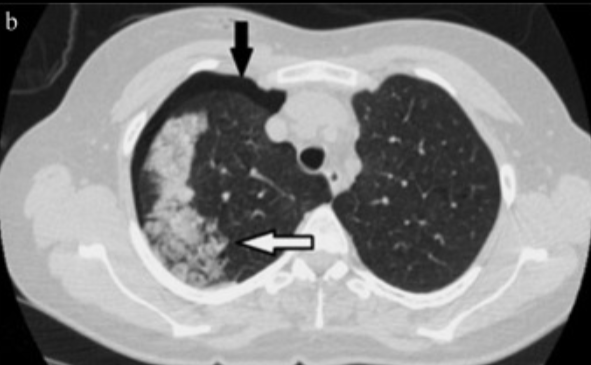
\includegraphics[width=0.7\textwidth]{img/complicacion.png}
    \caption{Neumotórax y hemorragia alveolar grado 2 como complicaciones tras la realización de una biopsia pulmonar guiada por TC \parencite{elshafee2019complications}.}
    \label{fig:complicaciones}
\end{figure}

Como se ha mencionado, hay numerosos estudios que aportan evidencia sobre la determinación de la benignidad o malignidad de distintos nódulos pulmonares, así como sobre la clasificación de diferentes tipos de neoplasias. Sin embargo, son escasos los trabajos que abordan el análisis de la probabilidad de desarrollar una complicación antes de realizar una biopsia.

Por ello, desarrollar modelos capaces de predecir el riesgo de complicaciones antes de la biopsia resulta especialmente relevante, ya que permitiría optimizar recursos médicos, planificar medidas preventivas y reducir la incidencia de eventos adversos.



\section{Propuesta}

Este trabajo propone el desarrollo de un sistema predictivo basado en técnicas de aprendizaje profundo y radiómica para anticipar el riesgo de complicaciones asociadas a biopsias pulmonares guiadas por TC. La idea central es construir un modelo capaz de analizar imágenes médicas tridimensionales junto con datos clínicos tabulares para estimar la probabilidad de complicaciones antes del procedimiento.

Para ello, se plantea integrar enfoques de radiómica y Deep Learning, que han demostrado un gran potencial en el análisis de imágenes médicas al facilitar la extracción automática de patrones complejos y mejorar la capacidad predictiva de los modelos \parencite{shen2017deep}. La radiómica ofrece un marco para extraer información cuantitativa de las imágenes, combinando características semánticas evaluadas por radiólogos con descriptores generados automáticamente. Este proceso requiere un flujo de trabajo estructurado que incluye la adquisición de las imágenes, la segmentación de las regiones de interés, la extracción de características y la construcción del modelo predictivo. Las Figuras~\ref{fig:compcaracteristicas_radiomica-label} y~\ref{fig:radiomica2-label} ilustran tanto la evolución de los tipos de características extraídas como el esquema general del flujo de trabajo que combina canales de radiómica convencional y aprendizaje profundo.

\begin{figure}[!htbp]
    \centering
    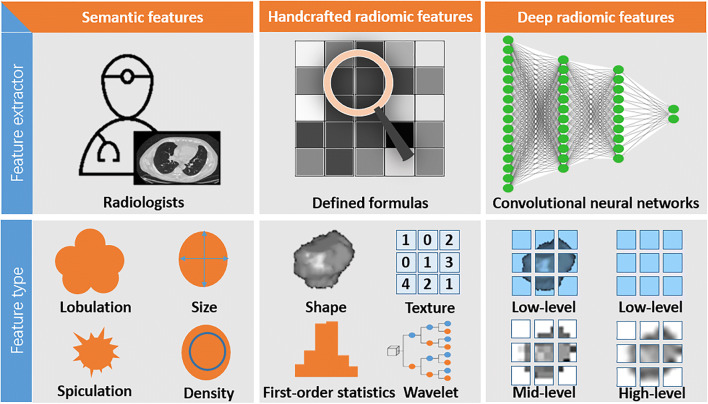
\includegraphics[width=0.9\textwidth]{img/comp_radiomica.jpg}
    \caption{Comparación de características semánticas, radiómicas manuales y radiómicas profundas \parencite{wu2021structural}.}
    \label{fig:compcaracteristicas_radiomica-label}
\end{figure}

\begin{figure}[!htbp]
    \centering
    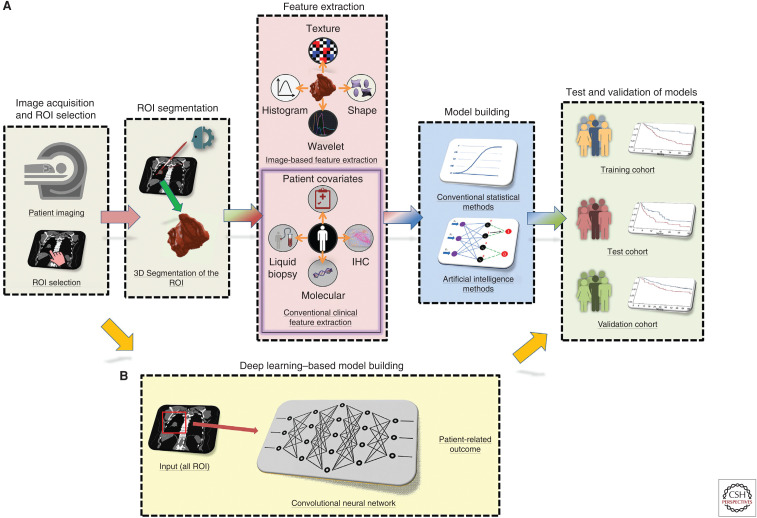
\includegraphics[width=1\textwidth]{img/radiomica2.jpg}
    \caption{Procesos de modelado de biomarcadores basados en imágenes. (A) Canal de radiómica convencional. (B) Canal de aprendizaje profundo. (ROI) Región de interés, (IHC) inmunohistoquímica \parencite{leiter2023global}.}
    \label{fig:radiomica2-label}
\end{figure}


Dada la ausencia de literatura previa en este campo concreto, la propuesta representa una línea de investigación novedosa. No existen modelos ni estrategias validadas para abordar la predicción del riesgo de complicaciones en biopsias pulmonares con inteligencia artificial (IA). Por ello, el diseño del presente estudio incluyó fases exploratorias para evaluar la viabilidad del enfoque, identificar limitaciones técnicas y comparar múltiples estrategias de modelado.

\section{Estructura del trabajo}
El contenido del trabajo se divide en dos partes:

\subsection*{Parte I: Matemáticas}

La primera parte proporciona el marco teórico y fundamento matemático necesario para entender las técnicas utilizadas en el la segunda parte. Comienza con la teoría de procesamiento de señales (Capítulo \ref{chap:señales}), donde se introducen conceptos fundamentales como la definición de señal, las transformadas de Fourier, la operación de convolución y la radiómica. A continuación, en  el Capítulo \ref{chap:optimizacion}, se abordan métodos de optimización basados en gradientes y optimización convexa, necesarios para garantizar la convergencia de los modelos.

En los fundamentos matemáticos del aprendizaje automático (Capítulo \ref{chap:aa-mates}), se detallan los tipos de aprendizaje (supervisado y no supervisado), centrándonos en el problema de clasificación. El aprendizaje profundo (Capítulo \ref{chap:dl-mates}) cubre la propagación hacia adelante, el algoritmo de backpropagation, las funciones de coste, las unidades de activación, el aprendizaje por transferencia y las redes neuronales convolucionales. Finalmente, los fundamentos métricos para el procesamiento avanzado de datos (Capítulo \ref{chap:metric-learning-mates}) profundizan en el aprendizaje de métricas de distancia, tanto en sus formulaciones lineales como no lineales.

\subsection*{Parte II: Informática}

La segunda parte aplica los conceptos teóricos para construir de forma práctica el sistema predictivo. Se inicia con el planteamiento del problema (Capítulo \ref{chap:planteamiento-problema}), donde se describe el contexto clínico, la motivación médica y las dificultades inherentes a la predicción de complicaciones en biopsias pulmonares. En el análisis de datos y preprocesamiento (Capítulo \ref{eda}), se detallan la adquisición, exploración y preparación de volúmenes TC mediante segmentación pulmonar, así como la normalización de datos clínicos tabulares.

El modelado con deep learning (Capítulo \ref{chap:dl-info}) incluye el desarrollo de arquitecturas 2D y 3D, estrategias avanzadas como el preentrenamiento, el fine-tuning y el aprendizaje contrastivo, además de la integración de datos clínicos e imágenes en modelos multimodales. En el análisis radiómico y machine learning clásico (Capítulo \ref{chap:aa-radiomica}) se abordan la extracción y el análisis de características radiómicas mediante técnicas de aprendizaje automático tradicional. El análisis experimental (Capítulo \ref{analisis-resultados}) describe la validación cruzada estratificada, el diseño de experimentos y el análisis detallado de resultados con métricas estándar. Finalmente, en el Capítulo \ref{chap:explicabilidad} se analizan los resultados con técnicas de explicabilidad, incluyendo métodos como Grad-CAM y SHAP, así como el análisis radiómico orientado a facilitar la interpretación y validación clínica de las predicciones.


\section{Objetivos}
Los objetivos inicialmente previstos en la propuesta del TFG fueron divididos en dos partes. 

En la parte de Matemáticas se persigue como objetivo fundamental proporcionar el soporte teórico necesario para entender las técnicas empleadas en el procesamiento y análisis de imágenes médicas. Para ello, se plantean los siguientes objetivos:

\begin{itemize}
    \item Estudiar los conceptos de señal, procesamiento de señales y teoría de radiómica.
    \item Comprender la teoría de optimización, incluyendo métodos basados en gradientes y propiedades de la convexidad.
    \item Analizar los fundamentos del aprendizaje automático y profundo, desde los principios básicos de clasificación hasta el funcionamiento de redes neuronales.
\end{itemize}


En la parte de Informática tiene como objetivo aplicar estos fundamentos para desarrollar de forma práctica el sistema predictivo. En este bloque se proponen los siguientes objetivos específicos:

\begin{itemize}
    \item Analizar y preprocesar datos clínicos tabulares y volúmenes de TC, incluyendo segmentación pulmonar, normalización y homogenización de datos para su uso en modelos.
    \item Desarrollar estrategias de modelado basadas en redes neuronales convolucionales 2D y 3D, definiendo arquitecturas, procedimientos de entrenamiento y estrategias avanzadas como el preentrenamiento y fine-tuning.
    \item Integrar datos clínicos con imágenes médicas para construir modelos multimodales capaces de aprovechar toda la información disponible.
    \item Aplicar técnicas de radiómica para extraer características relevantes de las imágenes y emplearlas en modelos clásicos de aprendizaje automático.
    \item Diseñar una experimentación adecuada que incluya validación cruzada estratificada para evaluar de manera robusta el rendimiento del sistema, mitigando problemas derivados del tamaño reducido de la muestra.
    \item Realizar un análisis detallado de los resultados, incorporando métricas estándar de evaluación y aplicando técnicas de explicabilidad para interpretar las predicciones y facilitar su validación clínica.
\end{itemize}


Finalmente, cabe señalar que los objetivos planteados se han cumplido en términos generales, logrando desarrollar un sistema predictivo funcional que integra las distintas etapas de procesamiento de datos, modelado y análisis. Sin embargo, los resultados obtenidos todavía muestran margen de mejora por varias razones. A lo largo del proyecto, la disponibilidad de datos fue aumentando de forma progresiva, lo que obligó a replantear y ajustar los experimentos en diferentes fases. Además, el conjunto inicial presentaba un fuerte desbalanceo entre clases que requirió técnicas específicas para mitigarlo. En general, el tamaño limitado del conjunto de datos redujo la capacidad de generalización de los modelos. Por último, el trabajo se llevó a cabo sin contar con una base de literatura consolidada específica para este problema clínico, lo que implicó diseñar soluciones desde cero y adaptar estrategias de problemas similares.



\section{Bibliografía fundamental}
A lo largo del trabajo se han consultado numerosas fuentes, pero entre ellas se puede destacar la siguiente bibliografía:

\begin{itemize}
    \item Goodfellow, I., Bengio, Y., Courville, A. y Bengio, Y. (2016). \textit{Deep learning} (Vol. 1, No. 2). Cambridge: MIT Press. Utilizada para el estudio de la teoría de optimización y los fundamentos de Deep Learning. 
    \item Shalev-Shwartz, S., y Ben-David, S. (2014). \textit{Understanding machine learning: From theory to algorithms}. Cambridge University Press. Utilizada para los fundamentos de aprendizaje automático y fundamentos del aprendizaje de métricas de distancias.
    \item Un artículo fundamental para el estudio de la radiómica y su base matemática: de Vaucleroy, N., Macq, B., De Vleeschouwer, C., y Léger, J. \textit{Mathematical morphology applied to Radiomics}.
    \item Artículos relacionados con la parte práctica aplicada a medicina: \cite{shur2021radiomics}, \cite{mukherjee2022radiomics}, \cite{suara2023grad}, \cite{calzado2010tomografia} y \cite{shen2017deep}. 
\end{itemize}



\endinput
 



% -------------------------------------------------------------------
% MAINMATTER
% -------------------------------------------------------------------
\mainmatter % activa la numeración de capítulos, resetea la numeración de las páginas y usa números arábigos

\part{Primera parte: Matemáticas} % Dividir un TFG en partes OPCIONAL

% Información relevante para la elaboración del trabajo.
% % !TeX root = ../tfg.tex
% !TeX encoding = utf8

\chapter{Documentación}\label{ch:primer-capitulo}

\section{Introducción}
Este documento es una plantilla para la elaboración de un trabajo fin de Grado siguiendo los \href{https://grados.ugr.es/matematicas/pages/infoacademica/tfg/requisitosTFG}{requisitos} de la comisión de Grado en Matemáticas de la Universidad de Granada que, a fecha de junio de 2023, son las siguientes:

\begin{itemize}
  \item La  memoria  debe  realizarse  con  un  procesador  de  texto  científico,  preferiblemente (La)TeX.
  \item La portada  debe contener  el  logo  de  la UGR,  incluir  el  título del TFG, el nombre del estudiante y especificar el grado, la facultad y el curso actual.
  \item La contraportada contendrá además el nombre del tutor o tutores.
  \item La memoria debe necesariamente incluir:
    \begin{itemize}
      \item Declaración explícita firmada en la que se asume la originalidad del trabajo, entendida en el sentido de que no ha utilizado fuentes sin citarlas debidamente. Esta declaración se puede descargar en la web del Grado.
      \item un índice detallado de capítulos y secciones,
      \item un resumen amplio en inglés del trabajo realizado (se recomienda entre 800 y 1500 palabras),
      \item una introducción en la que se describan claramente los objetivos previstos inicialmente en la propuesta de TFG, indicando si han sido o no alcanzados, los antecedentes importantes para el desarrollo, los resultados obtenidos, en su caso y las principales fuentes consultadas,
      \item una bibliografía final que incluya todas las referencias utilizadas.
    \end{itemize}
  \item Se recomienda que la extensión de la memoria sea de unas 50 páginas, sin incluir posibles apéndices.
\end{itemize}

Para generar el pdf a partir de la plantilla basta compilar el fichero \texttt{tfg.tex}. Es conveniente leer los comentarios contenidos en dicho fichero pues ayudarán a entender mejor como funciona la plantilla. 

La estructura de la plantilla es la siguiente\footnote{Los nombres de las carpetas no se han acentuado para evitar problemas en sistemas con Windows}: 
\begin{itemize}
  \item Carpeta \textbf{preliminares}: contiene los siguientes archivos
    \begin{description}
      \item[\texttt{dedicatoria.tex}] Para la dedicatoria del trabajo (opcional)
      \item[\texttt{agradecimientos.tex}] Para los agradecimientos del trabajo (opcional)
      \item[\texttt{introduccion.tex}] Para la introducción (obligatorio)
      \item[\texttt{summary.tex}] Para el resumen en inglés (obligatorio)
      \item[\texttt{tablacontenidos.tex}] Genera de forma automática la tabla de contenidos, el índice de figuras y el índice de tablas. Si bien la tabla de contenidos es conveniente incluirla, el índice de figuras y tablas es opcional. Por defecto está desactivado. Para mostrar dichos índices hay que editar este fichero y quitar el comentario a \verb+\listoffigures+ o \verb+\listoftables+ según queramos uno de los índices o los dos. En este archivo también es posible habilitar la inclusión de un índice de listados de código (si estos han sido incluidos con el paquete \texttt{listings})
  \end{description}
  El resto de archivos de dicha carpeta no es necesario editarlos pues su contenido se generará automáticamente a partir de los metadatos que agreguemos en \texttt{tfg.tex}

  \item Carpeta \textbf{capitulos}: contiene los archivos de los capítulos del TFG. Añadir tantos archivos como sean necesarios. Este capítulo es \texttt{capitulo01.tex}.

  \item Carpeta \textbf{apendices}: Para los apéndices (opcional)
  \item Carpeta \textbf{img}: Para incluir los ficheros de imagen que se usarán en el documento.
    
  \item Fichero \texttt{library.bib}: Para incluir las referencias bibliográficas en formato \texttt{bibtex}. Es útil la herramienta \href{https://www.doi2bib.org/}{doi2bib} para generar de forma automática el código bibtex de una referencia a partir de su \textsc{doi}  así como la base de datos bibliográfica \href{https://mathscinet.ams.org}{MathSciNet}. Para que una referencia aparezca en el pdf no basta con incluirla en el fichero \texttt{library.bib}, es necesario además \emph{citarla} en el documento usando el comando \verb+\cite+. Si queremos mostrar todos las referencias incluidas en el fichero \texttt{library.bib} podemos usar \verb+\cite{*}+ aunque esta opción no es la más adecuada. Se aconseja que los elementos de la bibliografía estén citados al menos una vez en el documento (y de esa forma aparecerán de forma automática en la lista de referencias).

  \item Fichero \texttt{glosario.tex}: Para incluir un glosario en el trabajo (opcional). Si no queremos incluir un glosario deberemos borrar el comando \verb+% !TeX root = ../tfg.tex
% !TeX encoding = utf8

\chapter*{Glosario}
\addcontentsline{toc}{chapter}{Glosario} % Añade el glosario a la tabla de contenidos


\begin{description}
  \item $\mathbb{R}$: Conjunto de números reales.
  \item $\mathbb{Z}$: Conjunto de números enteros.
  \item $\mathbb{R}^n$: Espacio euclídeo n-dimensional.
  \item $\mathbb{R}^{n \times m}$: Conjunto de matrices reales de tamaño $n \times m$.
  \item \textbf{TC}: Tomografía Computarizada
  \item \textbf{IA}: Inteligencia Artificial
  \item \textbf{BAG}: Biopsia por aguja gruesa
  \item \textbf{CT-guided PTNB}: Biopsia pulmonar transtorácica con aguja guiada por TC
  \item \textbf{MSE}: Error cuadrático medio (Mean Squared Error)
  \item \textbf{DFT}: Transformada Discreta de Fourier
  \item \textbf{FFT}: Transformada Rápida de Fourier
  \item \textbf{p.c.t}: para casi todo
  \item \textbf{c.p.d}: casi por doquier
  \item \textbf{ReLU}: Rectified Linear Units
  \item \textbf{PReLU}: Parametric ReLU
  \item \textbf{CNNs}: Convolutional Neural Networks
  \item \textbf{PCA}: Análisis de componentes principales (Principal Component Analysis)
  \item \textbf{NCA}: Neigborhood Components Analysis
  \item \textbf{LMNN}: Large Margin Nearest Neighbors
  \item \textbf{k-NN}: k-nearest neighbors
  \item \textbf{DML}: Aprendizaje de métricas profundo (Distance metric learning)
  \item \textbf{SVM}: Máquinas de vectores soporte (Support Vector Machines)
  \item \textbf{DICOM}: Digital Imaging and Communication in Medicine
  \item \textbf{NIfTI}: Neuroimaging Informatics Technology Initiative
  \item \textbf{RGPD}: Reglamento General de Protección de Datos (Reglamento (UE) 2016/679)
  \item \textbf{AEPD}: Agencia Española de Protección de Datos
  \item \textbf{EDA}: Análisis exploratorio de datos
  \item \textbf{GPUs}: Graphics Processing Units
  \item \textbf{MONAI}: Medical Open Network for Artificial Intelligence
  \item \textbf{IBSI}: Image Biomarker Standardisation Initiative
  \item \textbf{ROI}: Regiones de interés (Region of Interest)
  \item \textbf{VOI}: Volúmenes de interés (Volume of Interest)
  \item \textbf{HU}: Unidades Hounsfield
  \item \textbf{MLP}: Red neuronal multicapa (Multi-Layer Perceptron)
  \item \textbf{GLCM}: Matrices de co-ocurrencia de niveles de gris
  \item \textbf{GLDM}: Matriz de diferencia de niveles de gris
  \item \textbf{GLRLM}: Matrices de longitud de recorrido de niveles de gris
  \item \textbf{GLSZM}: Matriz de zonas de tamaño de niveles de gris
  \item \textbf{MPR}: Reformateo Multiplanar
  \item \textbf{TPR}: True Positive Rate (Sensibilidad)
  \item \textbf{TNR}: True Negative Rate (Especificidad)
  \item \textbf{DAG}: Grafo dirigido acíclico (Directed Acyclic Graph)
  \item \textbf{SHAP}: SHapley Additive exPlanations
  \item \textbf{TFG}: Trabajo de Fin de Grado
  \item \textbf{DL}: Deep Learning
  \item \textbf{ResNet}: Residual Networks
  \item \textbf{DenseNet}: Densely Connected Convolutional Network
  \item \textbf{CPU}: Procesador
  \item \textbf{UGR}: Universidad de Granada
  \item \textbf{NGPU}: Servidores de cómputo de alto rendimiento
  \item \textbf{WL}: Window Level
  \item \textbf{WW}: Window Width
  \item \textbf{IHC}: Inmunohistoquímica
  \item \textbf{DC}: Frecuencia cero, brillo medio en toda la imagen
\end{description}

\endinput

+ del fichero \texttt{tfg.tex} y posteriormente borrar el fichero \texttt{glosario.tex}

   \item Fichero \texttt{tfg.tex}: El documento maestro del TFG que hay que compilar con \LaTeX\ para obtener el pdf. En dicho documento hay que cambiar la \emph{información del título del \textsc{tfg} y el autor así como los tutores}.
\end{itemize}



\section{Elementos del texto}

En esta sección presentaremos diferentes ejemplos de los elementos de texto básico. Conviene consultar el contenido de \texttt{capitulos/capitulo01.tex} para ver cómo se han incluido.

\subsection{Listas}
En \LaTeX\ tenemos disponibles los siguientes tipos de listas:

Listas enumeradas:
\begin{enumerate}
  \item item 1
  \item item 2
  \item item 3
\end{enumerate}

Listas no enumeradas
\begin{itemize}
  \item item 1
  \item item 2
  \item item 3
  \end{itemize}

Listas descriptivas
\begin{description}
  \item[termino1] descripción 1
  \item[termino2] descripción 2
\end{description}
  
\subsection{Tablas y figuras}

En la \autoref{tb:ejemplo-tabla} o la \autoref{fig:logo-ugr} podemos ver\ldots

\begin{table}[htpb]
  \centering
  \begin{tabular}{ccc} \toprule
    \multicolumn{2}{c}{Agrupados} \\ \cmidrule(r){1-2}
    cabecera & cabecera & cabecera          \\ \midrule
    elemento & elemento & elemento          \\ 
    elemento & elemento & elemento          \\ 
    elemento & elemento & elemento          \\ \bottomrule
  \end{tabular}
  \caption{Ejemplo de tabla}
  \label{tb:ejemplo-tabla}
\end{table}

\begin{figure}[htpb]
  \centering
  
\includegraphics[width=0.5\textwidth]{logo-ugr}
  \caption{Logotipo de la Universidad de Granada}
  \label{fig:logo-ugr}
\end{figure}

\section{Entornos matemáticos}\label{sec:entornos-matematicos}

La plantilla tiene definidos varios entornos matemáticos cuyo nombre es el mismo omitiendo los acentos. Así, para incluir una \emph{proposición} usaríamos:

\begin{verbatim}
\begin{proposicion}
texto de la proposición
\end{proposicion} 
\end{verbatim}

Ver el código fuente del archivo \texttt{documentacion.tex} en la carpeta \texttt{capitulos} para el resto de ejemplos.

\begin{teorema}\label{thm:teorema}
Esto es un ejemplo de teorema.
\end{teorema}

\begin{proposicion}
Ejemplo de proposición
\end{proposicion}

\begin{lema}
Ejemplo de lema
\end{lema}

\begin{corolario}
Ejemplo de corolario
\end{corolario}

\begin{definicion}
Ejemplo de definición
\end{definicion}

\begin{observacion}
Ejemplo de observación
\end{observacion}

Adicionalmente está definido el entorno \texttt{teorema*} que permite incluir un teorema sin numeración:

\begin{teorema*}[Fórmula de Gauß-Bonnet]
  Sea $S$ una superficie compacta y $K$ su curvatura de Gauß. Entonces
\begin{equation}
  \int_S K = 2\pi\chi(S)
\end{equation}
donde $\chi(S)$ es la característica de Euler de $S$.
\end{teorema*}

Las fórmulas matemáticas se escriben entre símbolos de dólar \$ si van en línea con el texto o bien usando el entorno%
\footnote{
  También es posible delimitar una ecuación mediante los comandos \texttt{$\backslash$[} y \texttt{$\backslash$]} pero éstas nunca llevarán numeración aunque añadamos una etiqueta y las referenciemos (ver \autoref{sec:referencias}).
} 
\texttt{equation} cuando queremos que se impriman centradas en una línea propia, como el siguiente ejemplo
\begin{equation}\label{eq:identidad-pitagorica}
  \cos^2 x + \sin^2 x = 1.
\end{equation}


Gracias al paquete \texttt{mathtools}, las ecuaciones escritas dentro del entorno \texttt{equation} llevarán numeración de forma automática si son referenciadas  en cualquier parte del documento (por ejemplo la identidad Pitagórica~\eqref{eq:identidad-pitagorica}, ver el código de los dos anteriores ejemplos y la \autoref{sec:referencias} para más información sobre referencias cruzadas en el documento).

\section{Listados de código}

Podemos incluir un archivo externo de código mediante el comando \texttt{lstinputlisting} especificando su nombre completo (incluyendo la extensión) y usando la opción \texttt{inputpath} para indicar la ruta hacia el fichero (siempre referida a la carpeta principal de la plantilla) así como la opción \texttt{language} para indicar el lenguaje de programación en que está escrito (esto permitirá a \LaTeX\ colorear adecuadamente el código). Además, si lo consideramos necesario, podemos indicar las líneas que queremos mostrar (ver el código fuente del \autoref{code:prime}). Consultar todas las opciones posibles en la \href{https://osl.ugr.es/CTAN/macros/latex/contrib/listings/listings.pdf}{documentación del paquete \texttt{listings}}.

\lstinputlisting[inputpath=code, language=R, linerange={11-17}, firstnumber={11}, caption={Extracto código (líneas de 11 a 17) del fichero \texttt{primeR.r}}, label={code:prime}]{primeR.r}

Alternativamente, podemos incluir el código en un entorno \texttt{lstlisting} como el \autoref{code:perceptron}

\begin{lstlisting}[caption={Implementación de un perceptrón}, label={code:perceptron}, language={python}]
def dot(v, w):
    """Producto escalar de v y w, |$\color{comment}v_0 \cdot   w_0 + \cdots + v_n \cdot w_n$|"""
    return sum(v_i * w_i for v_i, w_i in zip(v, w))

def funcion_activacion(x):
    """1 si la entrada es mayor o igual que 1, 0 en otro caso."""
    return 1 if x >= 0 else 0

def perceptron(entrada, pesos):
    """1 si el perceptron se activa, 0 en otro caso"""
    return funcion_activacion(dot(entrada, pesos))
\end{lstlisting}

La opción \texttt{float} al incluir un listado de código permitará a dicho bloque ``flotar'' como si fuese un entorno \texttt{figure} y de esta manera evitaremos que se corte al final de una página.



\section{Referencias a elementos del texto}\label{sec:referencias}

Para las referencias a los elementos del texto (secciones, capítulos, teoremas,\ldots) se procede de la siguiente manera:
\begin{itemize}
  \item Se \emph{marca} el elemento (justo después del mismo si se trata de un capítulo o sección o en el interior del \emph{entorno} en otro caso), mediante el comando \verb+\label{+\emph{etiqueta}\verb+}+, donde \emph{etiqueta} debe ser un identificador único.
  \item Para crear una referencia al elemento en cualquier otra parte del texto se usa el comando \verb+\ref{+\emph{etiqueta}\verb+}+ (únicamente imprime la numeración asociada a dicho elemento, por ejemplo \ref{ch:primer-capitulo} o \ref{thm:teorema}) o bien \verb+\autoref{+\emph{etiqueta}\verb+}+ (imprime la numeración del elemento así como un texto previo indicando su tipo, por ejemplo \autoref{ch:primer-capitulo} o \autoref{thm:teorema})
\end{itemize}




\section{Bibliografía e índice}

Esto es un ejemplo de texto en un capítulo. Incluye varias citas tanto a libros~\cite{Aigner2018}, artículos de investigación~\cite{Euler1985}, recursos online~\cite{EulerWiki} (páginas web), tesis~\cite{CitekeyPhdthesis}, trabajo fin de máster~\cite{CitekeyMastersthesis}, trabajo fin de grado~\cite{CiteKeyBachelorsthesis} así como artículos sin publicar (preprints) \cite{castroinfantes2022conjugate} (en estos últimos usar el campo \texttt{note} para añadir la información relevante). 

Ver el fichero \texttt{library.bib} para las distintas plantillas. Cada nueva referencia debe añadirse en dicho fichero siguiendo el estilo del código \texttt{bibtex} según el tipo de referencia (página web, tesis, trabajo fin de grado o máster, artículo de investigación, libro,\ldots). Alternativamente se puede usar la web \href{https://zbib.org}{https://zbib.org} para generar automáticamente el código \texttt{bibtex}.


\endinput

% \chapter[Consideraciones elaboración TFG]{Consideraciones generales para la elaboración de un trabajo fin de grado}

\section{Normativa de la comisión del Grado en Matemáticas}

El \textsc{tfg} lo rigen dos normativas: 
\begin{itemize}
  \item una a nivel general de la UGR (\href{https://secretariageneral.ugr.es/sites/webugr/secretariageneral/public/inline-files/BOUGR/187/PLANTILLA%20CABECERASDoc2.pdf}{Reglamento del Trabajo o Proyecto fin de Grado de la Universidad de Granada}\footnote{\url{https://secretariageneral.ugr.es/sites/webugr/secretariageneral/public/inline-files/BOUGR/187/PLANTILLA\%20CABECERASDoc2.pdf}}) y 
  \item otra complementaria a nivel de la Facultad de Ciencias  (\href{https://fciencias.ugr.es/images/stories/documentos/reglamentos/reglamentoTfgCiencias23.pdf}{Reglamento del trabajo fin de grado en la Facultad de Ciencias de la Universidad de Granada}\footnote{\url{https://fciencias.ugr.es/images/stories/documentos/reglamentos/reglamentoTfgCiencias23.pdf}}). 
\end{itemize} 
Además, la comisión del Grado de Matemáticas impone unos \href{https://grados.ugr.es/matematicas/pages/infoacademica/tfg/requisitosTFG}{Requisitos de la memoria}\footnote{\url{https://grados.ugr.es/matematicas/pages/infoacademica/tfg/requisitosTFG}}.

El \textsc{tfg} hay que elaborarlo preferiblemente en LaTeX y puede usar la plantilla disponible en \href{https://github.com/latex-mat-ugr/Plantilla-TFG/archive/master.zip}{Plantilla \textsc{tfg} grado en matemáticas formato .tex}\footnote{\url{https://github.com/latex-mat-ugr/Plantilla-TFG/archive/master.zip}}.

Toda la información anterior puede encontrarse en la \href{https://grados.ugr.es/matematicas/pages/infoacademica/trabajofingrado}{web del Grado en Matemáticas}\footnote{\url{https://grados.ugr.es/matematicas/pages/infoacademica/trabajofingrado}}.

Es conveniente tener presente la documentación anterior para la elaboración del \textsc{tfg}. En especial en lo relativo a las fechas de depósito del \textsc{tfg} para su defensa.

A continuación destaco algunos aspectos importantes de la misma:
\begin{itemize}
\item El plagio, entendido como la presentación de un trabajo u obra hecho por otra persona como propio o la copia de textos sin citar su procedencia y dándolos como de elaboración propia, conllevará automáticamente la calificación numérica de cero. Esta consecuencia debe entenderse sin perjuicio de las responsabilidades disciplinarias en las que pudieran incurrir los estudiantes que plagien.
  \item Las memorias entregadas por parte de los estudiantes tendrán que ir firmadas sobre una declaración explícita en la que se asume la originalidad del trabajo, entendida en el sentido de que no ha utilizado fuentes sin citarlas debidamente.
\end{itemize}


% Los criterios de evaluación utilizados permitirán evaluar el grado de adquisición de las competencias que tiene establecidas el TFG en el VERIFICA de la titulación. Además, entre otros aspectos, se tendrá en consideración:

% \begin{itemize}
%   \item Redacción y ortografía tanto en la memoria del TFG como en los medios usados para la defensa del mismo (diapositivas, etc.).
%   \item Adecuación al formato de memoria indicado. Se proporcionará una plantilla de memoria de TFG a tal fin.
%   \item Adecuación temporal a los cronogramas de trabajo según los plazos de entrega marcados por el tutor/es.
%   \item Nivel de profundidad en los contenidos expuestos.
%   \item Dominio del tema e iniciativa del alumno.
%   \item Claridad de la exposición y adecuación al tiempo de exposición establecido.
%   \item Capacidad de análisis y síntesis.
%   \item Discusión con la Comisión Evaluadora en el turno de preguntas.
% \end{itemize}

% Se entregará una copia escrita, a doble cara, de la memoria del TFG para su evaluación, por parte de la Comisión Evaluadora, con una antelación de una semana (7 días naturales) antes de la fecha de defensa pública del TFG. Además, se entregará una versión en formato "pdf" de dicha memoria que quedará en la base de datos de todos los TFG y que custodiará la CTFGOO.




\section{Formato de la memoria}
La memoria se presentará usando un editor de textos científico, preferiblemente \LaTeX, e incluir los siguientes apartados:
\begin{enumerate}
  \item \emph{Resumen en inglés}: Deberá estar escrito completamente en inglés y tener una longitud recomendada entre 800 y 1500 palabras. 
  \item \emph{Introducción}. Deberá:
    \begin{itemize}
      \item Indicar los \emph{Objetivos del trabajo}: deberán aparecer con claridad los objetivos inicialmente previstos en la propuesta de \textsc{tfg} y los finalmente alcanzados con indicación de dificultades, cambios y mejoras respecto a la propuesta inicial. Si procede, es conveniente apuntar de manera precisa las interdependencias entre los distintos objetivos y conectarlos con los diferentes apartados de la memoria. Se pueden destacar aquí los aspectos formativos previos más utilizados. 
    \item Contextualizar el trabajo explicando antecedentes importantes para el desarrollo realizado y efectuando, en su caso, un estudio de los progresos recientes.
    \item Describir el problema abordado, de forma que el lector tenga desde este momento una idea clara de la cuestión a resolver o del producto a desarrollar y una visión general de la solución alcanzada.
    \item Indicar los resultados obtenidos.
    \item Citar las principales fuentes consultadas.
    \end{itemize}

  \item \emph{Desarrollo del trabajo}: El trabajo se estructurará en partes o capítulos según convengan, con la posibilidad de incluir apéndices. Se recomienda que la extensión de esta parte (sin incluir los apéndices) sea de unas 50 páginas. 

  \item \emph{Conclusiones y vías futuras}: Las conclusiones deberán incluir todas aquellas de tipo profesional y académico. Si hubiese posibles vías claras de desarrollo posterior sería interesante destacarlas aquí, poniéndolas en valor en el contexto inicial del trabajo.

  \item \emph{Bibliografía final}: Se incluirán tanto las fuentes primarias como todas aquellas cuyo peso haya sido menor en la realización del trabajo. Se recomienda un breve comentario de las referencias, ya sea individualizado, por grupos de referencias o global. En caso de incluir \textsc{url}s de páginas web deberán ir acompañadas de título, autor y fecha de último acceso, entre otros datos relevantes. Se recomienda no abusar de este tipo de fuentes.
\end{enumerate}




\section{Recomendaciones}
A la hora de abordar un trabajo como este, de cierta complejidad y extensión, es conveniente tener ciertas consideraciones desde un principio que ayuden a la organización y realización del mismo.
\begin{itemize}
    \item La memoria deberá ceñirse a las directrices dadas en la sección precedente. 
    
    \item Cualquier consulta externa (libro, artículo, página web, imagen,\ldots) debe estar debidamente referenciada tanto en el texto como en la bibliografía al final del trabajo. La bibliografía debe de aparecer en orden alfabético (del primer autor) en el formato indicado en la plantilla. 

    \item Se debe evitar copiar texto de forma literal, salvo citas literales, que se indicarán como tales y entrecomilladas. LaTeX proporciona el entorno \texttt{quote} para ello.

    \item Todas las imágenes y tablas incluidas en el documento deben figurar con su respectivos créditos (excepto que sean de elaboración propia). Por tanto, es recomendable guardar las referencias consultadas (direcciones web, libros) para la obtención de cualquier material gráfico o de datos.

    \item Si el trabajo contiene gran cantidad de vocabulario específico, conviene añadir un glosario de términos al final del mismo. Esto es mejor ir haciéndolo conforme se avanza en la redacción del trabajo.

    \item Es conveniente hacer un esquema inicial con la estructura general de la memoria: ¿de cuántas partes constará? ¿en qué orden? ¿qué incluirá cada una de ellas? En la plantilla proporcionada se recomienda una estructura general. Ello ayudará a organizar mejor el trabajo. No obstante, dicha estructura inicial puede ser modificada cuando el trabajo esté avanzado si el contenido lo requiere.
\end{itemize}


\input{capitulos/procesamiento_señales}
% !TeX root = ../tfg.tex
% !TeX encoding = utf8

\chapter{Optimización y convexidad} \label{chap:optimizacion}

En el contexto del aprendizaje automático, la optimización constituye una herramienta fundamental para minimizar funciones de pérdida y estimar parámetros de forma eficiente.

En este capítulo se presentan los conceptos esenciales de optimización y convexidad, que permiten garantizar la existencia y unicidad de soluciones bajo ciertas condiciones. Se estudian preliminares como el teorema de la proyección convexa y se introducen algoritmos basados en gradientes, que constituyen la base de los métodos de entrenamiento en los modelos que se abordarán en los capítulos posteriores.



\section{Preliminares}
Comenzamos con el teorema de la proyección convexa. Este teorema nos va a proporcionar una propiedad muy relevante sobre los conjuntos convexos, ampliamente utilizados en problemas de optimización.

\begin{teorema}[Teorema de la proyección convexa] 
Sea $X \subset \mathbb{R}^n$ convexo, no vacío y cerrado, y sea $y \in \mathbb{R}^n$. Entonces existe un único $\bar{x} \in X$ tal que $\|y - \bar{x}\| \leq \|y - x\|,\ \forall x \in X$. \label{teo:proyeccion-convexa}
\end{teorema}

\vspace{0.2cm}

\textit{Dem.} Sea $r > 0$ tal que $A := \overline{B}(y,r) \cap X$ no sea vacío. Nótese que $A$ es compacto por ser la intersección de un conjunto compacto y uno cerrado. Entonces la función $d_y$ definida por $d_y(x) = \|x - y\|$ alcanza su mínimo en $A$, ya que es una función continua; es decir, existe $\bar{x} \in A$ tal que $d_y(\bar{x}) \leq d_y(x)$ para todo $x \in A$.

\vspace{0.2cm}

Además, $\bar{x}$ es el mínimo de $d_y$ en $X$, pues si $x \in X \setminus \overline{B}(y,r)$ se tiene que $\|x - y\| > r \geq \|y - \bar{x}\|$.

\vspace{0.2cm}

Para demostrar la unicidad, supongamos que existen dos puntos $x_1, x_2$ de proyección de $y$. Por la convexidad de $X$, el punto medio $x = \frac{x_1 + x_2}{2}$ del segmento entre ellos también pertenece a $X$. Ahora, dado que $d_y(x_1) = d_y(x_2)$:

\[
\frac{1}{2} \langle x_1 - x_2, y - x \rangle = \frac{1}{2} \left\langle x_1 - x_2, y - \frac{1}{2}(x_1 + x_2) \right\rangle
\]
\[
= \frac{1}{4} \langle (y - x_2) - (y - x_1), (y - x_1) + (y - x_2) \rangle
\]
\[
= \frac{1}{4} \left( \|y - x_1\|^2 - \|y - x_2\|^2 \right) = 0
\]

\vspace{0.2cm}

Por el teorema de Pitágoras se verifica que $\|y - x\|^2 + \left\|\frac{x_1 - x_2}{2}\right\|^2 = \|y - x_2\|^2$ y teniendo en cuenta que $x - x_2 = \frac{x_1 - x_2}{2}$ se obtiene la igualdad

\[
\|y - x\|^2 + \|x - x_2\|^2 = \|y - x_2\|^2
\]

\vspace{0.2cm}

de modo que $\|y - x\|^2 \leq \|y - x_2\|^2$. La igualdad se da si, y solo si, $x = x_2$, por lo que $x_1 = x_2$. \hfill $\Box$

Este $\bar{x}$ se llama \textit{proyección convexa} de $y$ sobre $X$ y se denotará por $P_X(y)$.



\section{Algoritmos de optimización basados en gradientes}
La mayoría de los algoritmos de aprendizaje implican algún tipo de optimización. La optimización se refiere a la tarea de minimizar o maximizar alguna función $f(x)$ mediante la alteración de $x$. Solemos plantear la mayoría de los problemas de optimización en términos de minimización de $f(x)$. La maximización puede lograrse mediante un algoritmo de minimización minimizando $-f(x)$.

La función que queremos minimizar o maximizar se llama función objetivo o criterio. Cuando la estamos minimizando, también podemos llamarla función de coste, función de pérdida o función de error. 

A menudo denotamos el valor que minimiza (o maximiza) la función con un superíndice *. Por ejemplo:

\[
x^* = \arg\min_x f(x).
\]

Es habitual trabajar con funciones objetivo diferenciables y aprovechar las propiedades del gradiente para optimizar el valor de la función objetivo. A continuación se describe la base fundamental de estos métodos: el gradiente descendente. También se discute cómo optimizar funciones definidas en conjuntos con restricciones convexas.

\subsection{Descenso de gradiente}
Es conocido que el gradiente de una función diferenciable tiene la dirección de la máxima pendiente en el grafo de la función, por lo que avanzando pequeñas cantidades en la dirección opuesta a la del gradiente conseguimos reducir el valor de la función. Este método iterativo es el que se conoce como gradiente descendente.

Analicemos más en profundidad el gradiente descendente, un método clásico para la minimización de funciones. 

La regla de actualización de este método iterativo, para encontrar un $x \in \mathbb{R}^d$ que minimice una función objetivo diferenciable $f : \mathbb{R}^d \to \mathbb{R}$ viene dada por 
\[
x_{t+1} = x_t - \eta \nabla f(x_t), \quad t \in \mathbb{N} \cup \{0\},
\]
donde $\eta$ es la cantidad que se avanza en la dirección del gradiente, y se denomina tasa de aprendizaje. Dicho $\eta$ puede ser constante o puede ir adaptándose de acuerdo con las evaluaciones de la función objetivo. En el primer caso, la elección de un $\eta$ demasiado grande o demasiado pequeño puede conducir a malos resultados. El segundo caso requiere evaluar la función objetivo en cada iteración, lo que puede ser costoso computacionalmente.

\vspace{0.3cm}

Los fundamentos del gradiente descendente se basan en las siguientes ideas. Consideramos una función objetivo $f : \mathbb{R}^d \to \mathbb{R}$, $x \in \Omega$ y $v \in \mathbb{R}^d \setminus \{0\}$ una dirección arbitraria. Consideramos la función $g: \mathbb{R} \to \mathbb{R}$ dada por 
\[
g(\eta) = f(x + \eta \frac{v}{\|v\|}).
\]
La tasa de variación o derivada direccional de $f$ en $x$ para la dirección $v$ viene dada por 
\[
g'(0) = \frac{1}{\|v\|} \langle \nabla f(x), v \rangle.
\]
Aplicando la desigualdad de Cauchy-Schwarz, se tiene
\[
- \|\nabla f(x)\| \leq \frac{1}{\|v\|} \langle \nabla f(x), v \rangle \leq \|\nabla f(x)\|,
\]
y la igualdad en la desigualdad izquierda se alcanza cuando $v = -\nabla f(x)$, obteniendo así la tasa máxima de descenso. De la misma forma, la tasa de máximo ascenso se alcanza con $\nabla f(x)$.

\vspace{0.3cm}

Si el gradiente en $x$ es no nulo, y consideramos la aproximación de Taylor de primer orden para los puntos $x - \eta \nabla f(x)$, se tiene
\[
f(x - \eta \nabla f(x)) = f(x) - \eta \|\nabla f(x)\|^2 + o(\eta),
\]
con $\lim_{\eta \to 0} \frac{o(\eta)}{\eta} = 0$, luego existe $\varepsilon > 0$ tal que si $0 < \delta < \varepsilon$, se tiene
\[
\frac{o(\delta)}{\delta} < \|\nabla f(x)\|,
\]
y por tanto,
\[
f(x - \delta \nabla f(x)) - f(x) = \delta \left( -\|\nabla f(x)\|^2 + \frac{o(\delta)}{\delta} \right) < \delta \left( -\|\nabla f(x)\|^2 + \|\nabla f(x)\| \right) = 0.
\]

luego $f(x - \delta \nabla f(x)) < f(x)$ para $0 < \delta < \varepsilon$, luego tenemos garantizado que para una tasa de aprendizaje adecuada el método puede descender en cada iteración. 

Podemos observar que la dirección del gradiente no es la única dirección de descenso válida, sino que lo anterior sigue siendo válido para cualquier dirección $v \in \mathbb{R}^d$ con $\langle \nabla f(x), v \rangle < 0$. La elección de otras direcciones de descenso, aunque no sean las de máxima pendiente, pueden proporcionar mejores resultados en problemas determinados.

\vspace{0.3cm}

Cuando trabajamos con problemas de optimización con restricciones, el método del gradiente no puede ser aplicado directamente, pues la regla de adaptación $x_{t+1} = x_t - \eta \nabla f(x_t)$ no garantiza que $x_{t+1}$ sea un punto viable. El método del gradiente con proyecciones soluciona este problema, cuando el problema de optimización es convexo, añadiendo una proyección sobre el conjunto viable en la regla de adaptación, es decir, si $C$ es el conjunto convexo determinado por las restricciones (que supondremos también cerrado, esta condición se tiene cuando las funciones restricción son continuas, y la convexidad garantiza la continuidad en el interior del dominio), y $P_C$ es la proyección sobre dicho conjunto, entonces la regla de adaptación se convierte en
\[
x_{t+1} = P_C(x_t - \eta \nabla f(x_t)).
\]
Para confirmar la validez de este método, tenemos que ver que la dirección $v = P_C(x - \eta \nabla f(x)) - x$ es una dirección de descenso, lo cual, por lo razonado anteriormente, se consigue si $\langle \nabla f(x), v \rangle < 0$.

\vspace{0.3cm}

Llamamos $x_1 = x - \eta \nabla f(x)$. Entonces, $v = P_C(x_1) - x$. Notemos que $\langle \nabla f(x), v \rangle < 0 \implies \langle x - x_1, P_C(x_1) - x \rangle = -\eta \langle \nabla f(x), v \rangle > 0$. Si el gradiente es no nulo y $x_1 \in C$, entonces $\langle x - x_1, x - x_1 \rangle = \|x_1 - x\|^2 > 0$. 

Si $x_1 \notin C$, entonces el teorema de la proyección convexa \ref{teo:proyeccion-convexa} asegura que el semiespacio 
\[
H = \{ y \in \mathbb{R}^d : \langle x_1 - P_C(x_1), y - P_C(x_1) \rangle \leq 0 \}
\]
contiene a $C$. En particular,
\[
0 \geq \langle x_1 - P_C(x_1), x - P_C(x_1) \rangle = \langle x_1 - x, x - P_C(x_1) \rangle + \|x - P_C(x_1)\|^2.
\]

\vspace{0.3cm}

En consecuencia, $\langle x_1 - x, P_C(x_1) - x \rangle \geq \|x - P_C(x_1)\|^2 \geq 0$. Además, la igualdad se da si y solo si $x = P_C(x_1)$, y en tal caso el algoritmo habrá convergido (observemos que esto ocurre cuando $x \in \text{Fr } C$ y la dirección de descenso proporcionada por el gradiente apunta hacia fuera de $C$ y de forma ortogonal al hiperplano soporte). Por tanto, mientras las iteraciones del gradiente con proyecciones provoquen algún movimiento en los puntos obtenidos, escogiendo la tasa de aprendizaje adecuada, tenemos la garantía de poder descender en la función objetivo.  En la Figura \ref{fig:convergencia} se pueden comparar visualmente el gradiente con proyecciones y el gradiente descendente.

\begin{figure}[!htbp]
    \centering
    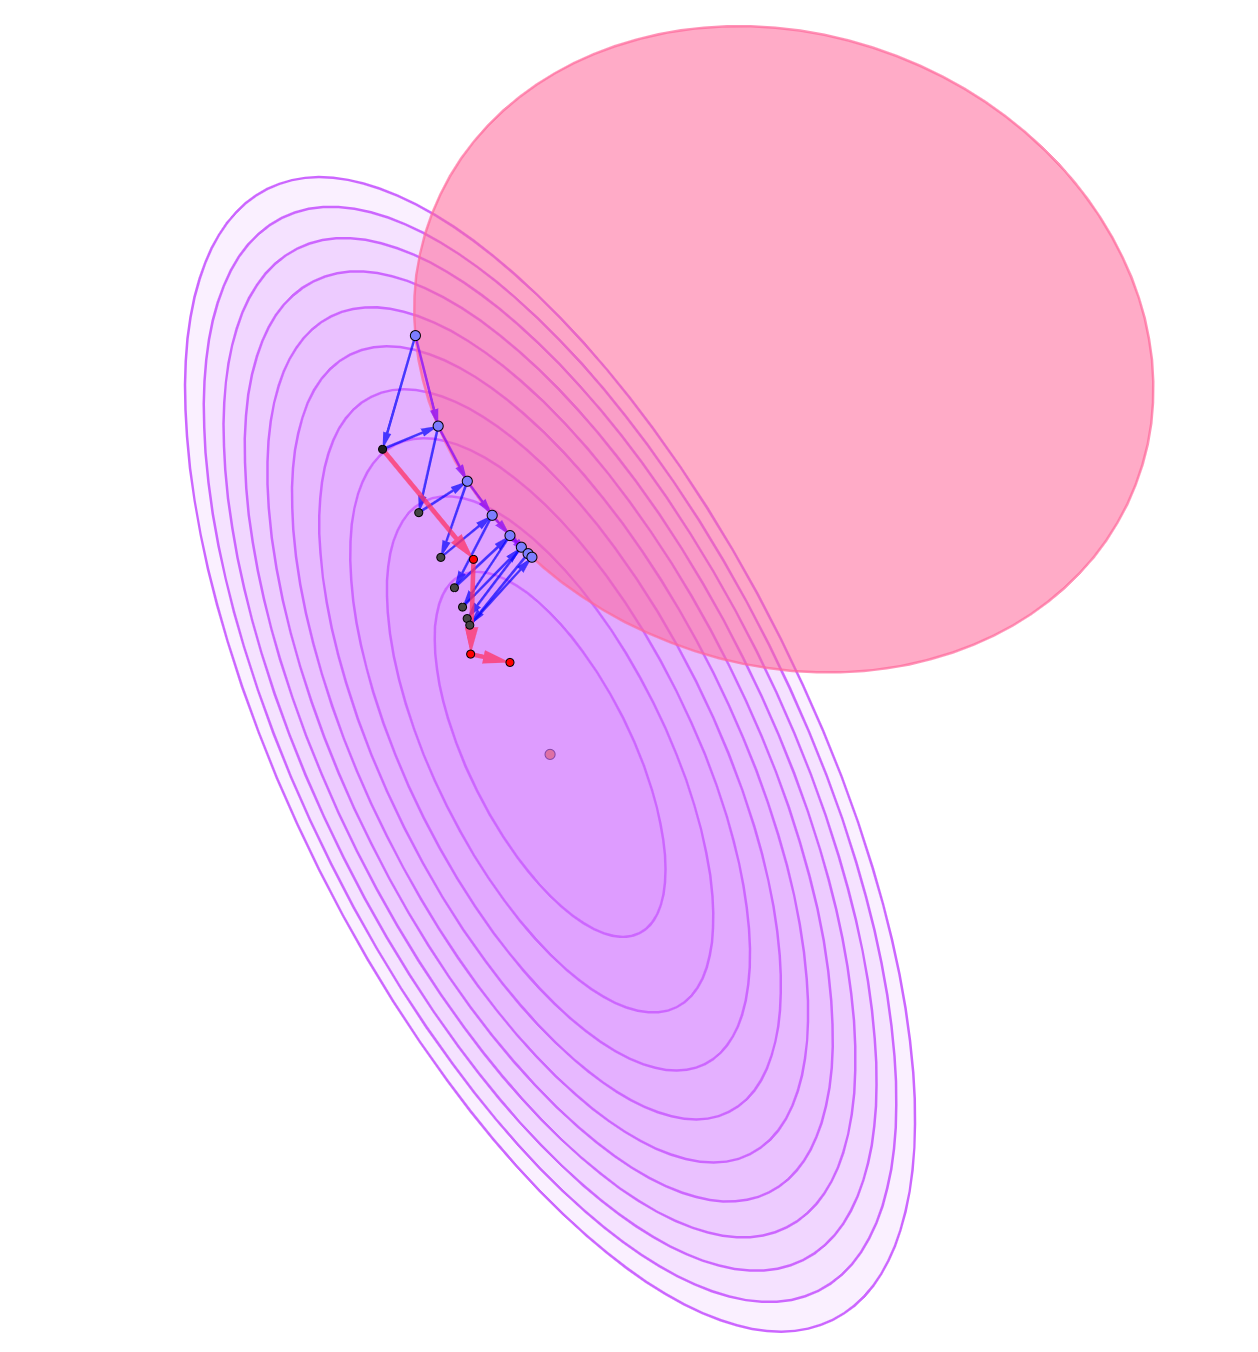
\includegraphics[width=0.8\textwidth]{img/convergencia.png}
    \caption{Curvas de nivel de una función objetivo a optimizar (morado). Gradiente descendente (recorrido rojo) y gradiente descendente con proyecciones sobre un conjunto convexo (azul). Se puede observar que el recorrido que se sigue sobre el conjunto convexo también minimiza la función objetivo.}
    \label{fig:convergencia}
\end{figure}

\subsection{Jacobiano y Hessiano}

Cuando la función tiene entradas y salidas vectoriales, usamos la \emph{matriz Jacobiana}. Para \( f : \mathbb{R}^n \to \mathbb{R}^m \), con \( f = (f_1, f_2, \ldots, f_m) \), el Jacobiano en un punto \( x \in \mathbb{R}^n \) se define como:

\[
J_f(x) = 
\begin{pmatrix}
\frac{\partial f_1}{\partial x_1}(x) & \frac{\partial f_1}{\partial x_2}(x) & \cdots & \frac{\partial f_1}{\partial x_n}(x) \\
\frac{\partial f_2}{\partial x_1}(x) & \frac{\partial f_2}{\partial x_2}(x) & \cdots & \frac{\partial f_2}{\partial x_n}(x) \\
\vdots & \vdots & \ddots & \vdots \\
\frac{\partial f_m}{\partial x_1}(x) & \frac{\partial f_m}{\partial x_2}(x) & \cdots & \frac{\partial f_m}{\partial x_n}(x)
\end{pmatrix}
=
\begin{pmatrix}
\nabla f_1(x) \\
\vdots \\
\nabla f_m(x)
\end{pmatrix},
\]

donde \(\nabla f_i(x)\) es el \emph{gradiente} de la i-ésima componente escalar.

La \emph{segunda derivada} o \emph{Hessiano} se usa para funciones \( f : \mathbb{R}^n \to \mathbb{R} \). Su definición es:

\[
H_{i,j} = \frac{\partial^2 f}{\partial x_i \partial x_j}.
\]

El Hessiano es \emph{simétrico} si las segundas derivadas son continuas.

\begin{itemize}
  \item Si el Hessiano es positivo definido, el punto es un mínimo local.
  \item Si es negativo definido es un máximo local.
  \item Si tiene valores propios positivos y negativos, es un punto de silla.
\end{itemize}


\subsubsection{Número de condición del Hessiano}
El \emph{número de condición} del Hessiano indica las diferencias entre las curvaturas en distintas direcciones. Un número de condición alto dificulta el descenso por gradiente porque en una dirección la derivada puede crecer rápido yn otra dirección puede crecer lento. Esto obliga a elegir tasas de aprendizaje pequeñas, ralentizando la convergencia.

\subsection{Optimización Convexa}

En \emph{optimización convexa}, la función tiene Hessiano \emph{semidefinido positivo} en todas partes:

\begin{itemize}
  \item No hay puntos de silla.
  \item Todos los mínimos locales son mínimos globales.
\end{itemize}

En muchos algoritmos de aprendizaje automático se busca que la optimización sea convexa para asegurar que se alcanza un mínimo global. 


\endinput
%--------------------------------------------------------------------
% FIN DEL CAPÍTULO. 
%--------------------------------------------------------------------

% !TeX root = ../tfg.tex
% !TeX encoding = utf8

\chapter{Fundamentos matemáticos del aprendizaje automático} \label{chap:aa-mates}
En este capítulo se abordarán los conceptos fundamentales del aprendizaje automático. Se comenzará por definir formalmente qué significa aprender para un sistema informático y se describirán las principales modalidades de aprendizaje automático, como el aprendizaje supervisado y no supervisado. A partir de estas bases, se introducirán conceptos clave como el problema de clasificación.



\section{Concepto de Aprendizaje Automático}

El Aprendizaje Automático se encarga de aprender de datos a través de un algoritmo o programa informático. Vamos a definir que se considera como aprender según \cite{mitchell1997machine}: 

\begin{definicion}
Un programa informático aprende de la experiencia E con respecto a una clase de tareas T y una medida de rendimiento P, si su rendimiento en tareas de T, medido por P, mejora con la experiencia E.
\end{definicion}

El aprendizaje automático permite abordar tareas que son demasiado complejas para ser resueltas con programas fijos diseñados manualmente por seres humanos. La tarea es el tipo de problema a resolver. Actualmente hay una inmensidad de posibilidades y problemas a resolver (clasificación, regresión, transcripción, traducción, detección de anomalías, imputación de valores faltantes, etc.). La tarea define lo que se espera que el modelo aprenda a hacer. Por ejemplo, puede tratarse de clasificar imágenes médicas según la presencia o ausencia de una enfermedad, predecir el precio de una vivienda o reconocer voz humana. 

La medida de rendimiento (P) es la forma en la que evaluamos cualitativamente la capacidad del modelo en la tarea T. Dependiendo del tipo de tarea es más informativa una u otra medida que nos permite cuantificar si el sistema está mejorando a medida que entrena con más experiencia. Algunas métricas comunes son: precisión (Accuracy) que se utiliza comúnmente para tareas de clasificación, error cuadrático medio (Mean Squared Error, MSE) para tareas de regresión, F-score, precisión, recall ...

Por último, la experiencia (E) son los datos con el que sistema aprende. Constituyen la base a partir de la cual el modelo extrae patrones y lo generaliza. Cuanto más rica y representativa sea la experiencia, mejor podrá el modelo aprender. Los algoritmos de aprendizaje automático se clasifican ampliamente según el tipo de experiencia que se les permite tener durante el proceso de aprendizaje. 



\section{Tipos de aprendizaje automático}
El campo de aprendizaje es muy amplio. Por consiguiente, el aprendizaje automático se ha dividido en varios subcampos para estudiar los distintos tipos de tareas de aprendizaje. 

Una taxonomía general en función de la experiencia E es dividir el aprendizaje automático entre aprendizaje supervisado y no supervisado. 

\subsection{Aprendizaje supervisado}
Este tipo de aprendizaje implica algoritmos que aprenden a asociar alguna entrada con alguna salida, dado un conjunto de entrenamiento de ejemplos que incluyen tanto las entradas ($x$) como sus correspondientes salidas o \textit{etiquetas} ($y$). A continuación determinamos las características de este aprendizaje:

\begin{itemize}
    \item Datos de entrenamiento: Cada ejemplo en el conjunto de datos está asociado con una etiqueta. 
    \item Objetivo: El objetivo principal es predecir y a partir de $x$, lo que generalmente se logra estimando la distribución de probabilidad condicional $p(y|x)$.
    \item Tareas comunes: Tradicionalmente, se consideran tareas de aprendizaje supervisado la regresión (predecir un valor numérico), la clasificación (predecir una categoría) y los problemas de salida estructurada (predecir una secuencia o estructura más compleja). Un ejemplo de regresión es predecir un valor y a partir de x usando una función lineal, como en la regresión lineal.
    \item Modelos probabilísticos: Muchos algoritmos de aprendizaje supervisado se basan en estimar $p(y|x)$ utilizando la estimación de máxima verosimilitud para encontrar el mejor vector de parámetros $\theta$ para una familia paramétrica de distribuciones.
\end{itemize}


Vamos a formalizar el enfoque siguiendo a \cite{shalev2014understanding}, explicando los elementos de un algoritmo de aprendizaje supervisado. Como entrada del algoritmo se definen los siguientes componentes:

\begin{itemize}
    \item \textbf{Conjunto de dominio} $\mathcal{X}$: es un conjunto arbitrario de objetos (también llamados \emph{instancias}) que se desea etiquetar denominado como $\mathcal{X}$. Los elementos de $\mathcal{X}$ se representan mediante vectores de características.
    
    \item \textbf{Conjunto de etiquetas} $\mathcal{Y}$: es otro conjunto arbitrario, esta vez finito de posibles etiquetas. 
    
    \item \textbf{Conjunto de los datos de entrenamiento} $S = \{(x_1, y_1), \ldots, (x_m, y_m)\} \subseteq \mathcal{X} \times \mathcal{Y}$: secuencia finita de pares instancia-etiqueta. Este es el conjunto de datos etiquetados que se proporciona al algoritmo.
\end{itemize}

El objetivo del aprendizaje es generar una \textit{regla de predicción} o \emph{hipótesis} $h: \mathcal{X} \to \mathcal{Y}$ que, dada una nueva instancia $x \in \mathcal{X}$, sea capaz de predecir correctamente su etiqueta. 

Para modelar el problema se asume que los datos $(x_i, y_i)$ están generados siguiendo una determinada distribución de probabilidad $D$ sobre $\mathcal{X}$ y una función de etiquetado desconocida $f: \mathcal{X} \to \mathcal{Y}$, tal que $y_i = f(x_i)$.


El rendimiento del clasificador $h$ se mide mediante su \textit{error de generalización} respecto a $D$ y $f$, definido como:

\begin{equation}
L_{D, f}(h) \overset{\text{def}}{=} \mathbb{P}_{x \sim D} \left[ h(x) \neq f(x) \right]
\end{equation}

Este valor representa la probabilidad de que $h$ cometa un error al predecir la etiqueta de una instancia $x$ tomada al azar según $D$.

El objetivo del aprendizaje es minimizar esta cantidad, es decir, encontrar una función $h$ que generalice bien sobre datos no vistos.


\subsection{Aprendizaje no supervisado} 
Los algoritmos de aprendizaje no supervisado son aquellos que solo reciben \emph{características} (x) pero no una señal de supervisión o etiquetas. Las características principales son: 

\begin{itemize}
    \item \textbf{Datos de entrenamiento}: Solo se observan ejemplos de un vector aleatorio $x$, sin etiquetas asociadas.
    \item \textbf{Objetivo}: Intentar aprender implícita o explícitamente la distribución de probabilidad $p(x)$ o algunas propiedades interesantes de esa distribución. El objetivo clásico es encontrar la \emph{mejor} representación de los datos, lo que implica preservar la mayor cantidad de información posible sobre $x$ mientras se mantienen propiedades deseables como menor dimensionalidad, escasez o independencia en la representación.
    \item \textbf{Tareas comunes}: Estimación de densidad (modelar la distribución de los datos), aprender a extraer muestras de una distribución, quitar ruido de datos (denoising), encontrar una variedad (manifold) cercana a la que se encuentran los datos, o agrupar los datos en clusters de ejemplos relacionados.
\end{itemize}

Además del aprendizaje no supervisado clásico, existen otras variantes del paradigma en distintos contextos. Por ejemplo, el aprendizaje semisupervisado combina datos etiquetados y no etiquetados para mejorar la generalización cuando las etiquetas son escasas o costosas de obtener. El aprendizaje multiinstancia permite entrenar modelos cuando las etiquetas no están disponibles para instancias individuales, sino para conjuntos o bolsas de instancias, siendo útil en dominios como la histopatología o la visión por computador. Las reglas de decisión son estrategias formales para definir cómo un modelo toma decisiones basadas en los datos, estableciendo criterios claros y sistemáticos que facilitan la interpretación y la implementación de los resultados del aprendizaje. Por último, el aprendizaje por refuerzo consiste en entrenar un agente que aprende a tomar decisiones secuenciales a través de la interacción con un entorno, optimizando una señal de recompensa acumulada en el tiempo, y se utiliza en aplicaciones que van desde robótica hasta videojuegos o sistemas de recomendación.

\section{Problema de clasificación}
El problema de clasificación consiste en aprender una función (clasificador) que asigne a cada dato en el dominio $\mathcal{X}$ una clase de entre un conjunto finito de clases, que conforman $\mathcal{Y}$. El problema de clasificación más común es el binario, donde el conjunto $\mathcal{Y}$ tiene solo dos elementos. Se suele representar en estos casos $\mathcal{Y} = \{-1,1\}$ o $\mathcal{Y} = \{0,1\}$. La clasificación binaria es de gran importancia, pues cualquier otro problema de clasificación puede reducirse a subproblemas de clasificación binaria. Muchos algoritmos de clasificación trabajan, por tanto, con problemas binarios, y reducen los problemas con más clases a subproblemas de este tipo. Los problemas de clasificación con más de dos clases se conocen como multiclase. 

Los problemas de clasificación tienen gran cantidad de aplicaciones en ámbitos muy variados, como por ejemplo, la detección de enfermedades, el reconocimiento de imágenes o sonidos, la detección de correos de spam, el desarrollo de motores de búsqueda en Internet, la taxonomía dentro de la biología o la clasificación de documentos.









\endinput
%--------------------------------------------------------------------
% FIN DEL CAPÍTULO. 
%--------------------------------------------------------------------

% !TeX root = ../tfg.tex
% !TeX encoding = utf8

\chapter{Fundamentos matemáticos del aprendizaje profundo} \label{chap:dl-mates}
Posteriormente, después de haber sentado las bases del aprendizaje automático, vamos a profundizar en las redes neuronales artificiales y en el aprendizaje profundo como aproximación avanzada capaz de modelar funciones complejas. Se explicarán los fundamentos matemáticos necesarios para su entrenamiento, incluidos los algoritmos de optimización basados en gradiente y el algoritmo de retropropagación. Finalmente, se discutirán aspectos avanzados como la selección de funciones de coste, tipos de unidades de salida y ocultas, así como conceptos de transferencia de aprendizaje y redes neuronales convolucionales, incluyendo las operaciones de convolución y pooling.

Aunque los algoritmos clásicos de aprendizaje automático han demostrado ser eficaces en muchos problemas relevantes, no han sido capaces de abordar con éxito algunos de los grandes retos de la inteligencia artificial, como el reconocimiento de voz o la identificación automática de objetos en imágenes. Uno de los principales motivos es la dificultad para generalizar correctamente cuando se trabaja con datos de alta dimensión, donde los métodos tradicionales suelen fallar o requerir un esfuerzo computacional elevado. Además, las técnicas clásicas carecen de la capacidad de representar funciones complejas necesarias en estos entornos. En respuesta a estas limitaciones, surge el aprendizaje profundo (deep learning), una rama del aprendizaje automático que introduce arquitecturas más potentes y mecanismos adaptativos con el objetivo de aprender representaciones útiles y eficaces incluso en espacios de gran complejidad.

Una red neuronal artificial (RNA) se inspira en la estructura de las redes neuronales del cerebro \parencite{Goodfellow-et-al-2016}. Una RNA consiste en un conjunto de funciones elementales conectadas entre sí, donde cada función procesa entradas y transmite una salida a otras unidades. Estas redes se estructuran como grafos dirigidos acíclicos, donde los nodos representan neuronas y las aristas conexiones con pesos asociados. Una red neuronal define una función $y = f(x; \theta)$ que aprende los parámetros $\theta$ para busca aproximar una función objetivo $f^*$, utilizando una sucesión de transformaciones funcionales compuestas. Esta composición se puede expresar como:

\begin{equation}
f(x) = f^{(L)}(f^{(L-1)}(\dots f^{(1)}(x)))
\end{equation}

Su estructura se define por capas de unidades (\textit{neuronas}) interconectadas. En la Figura \ref{fig:red-neuronal} tenemos un ejemplo de una red neuronal feedfoward. La longitud de la cadena determina la \textit{profundidad} del modelo, de ahí el término \textit{aprendizaje profundo} o \textit{deep learning}:
\begin{itemize}
    \item \textbf{Capa de entrada}: Recibe los valores iniciales de $\mathbf{x}$. Son las capas más situadas a la izquierda en que se encuentran las neuronas de entrada, las cuales se encargan de percibir los datos recibidos a través de las entradas.
    \item \textbf{Capas ocultas}: Son capas intermedias de neuronas. El comportamiento de estas capas no está especificado por los datos. El algoritmo de aprendizaje debe decidir cómo utilizar estas capas para producir la salida deseada, pero los datos no indican qué debe hacer cada capa individual. Por tanto, el algoritmo debe encontrar la mejor manera de usar estas capas para aproximar la función $f^*$.
    \item \textbf{Capa de salida}: Son las capas más situadas a la derecha. Produce el resultado final de la red. Si la salida es un valor continuo (regresión), puede usarse una función de activación lineal o sigmoide. Para clasificación, se suelen usar funciones como softmax para probabilidades multinomiales.
\end{itemize}

Durante el entrenamiento de una red neuronal, se busca que la función aprendida $f(x)$ se aproxime a una función objetivo $f^*(x)$. Los datos de entrenamiento nos proporcionan ejemplos aproximados de $f^*(x)$ evaluados en distintos puntos. Cada ejemplo $x$ está asociado a una etiqueta $y \approx f^*(x)$.


\begin{figure}[!htbp]
    \centering
    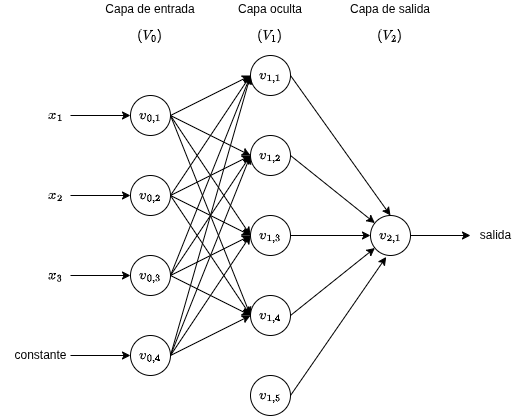
\includegraphics[width=0.8\textwidth]{img/red_neuronal.png}
    \caption{Red neuronal feedforward en capas de profundidad 2, tamaño 10 y anchura 5. Hay una neurona en la capa oculta que no tiene aristas entrantes. Además, hay una neurona en la capa oculta que no tiene aristas entrantes. La salida de esta neurona será $f^{(1)}(0)$, es decir, la función de activación evaluada en $0$. Elaboración propia. }
    \label{fig:red-neuronal}
\end{figure}


Una forma de entender el papel de las redes neuronales es partir de las limitaciones de los modelos lineales clásicos, como la regresión lineal o logística. Estos modelos son muy útiles por su simplicidad y eficiencia, pero tienen un problema fundamental: solo pueden capturar relaciones lineales entre las variables de entrada, lo que limita su capacidad para modelar fenómenos complejos del mundo real.

Para superar esta limitación, la idea es aplicar el modelo lineal no directamente sobre la entrada original \(x\), sino sobre una transformación no lineal de los datos, denotada por \(\phi(x)\). Así, en lugar de aprender una función lineal en el espacio original, se aprende una función lineal en un espacio transformado donde las relaciones sean más sencillas de modelar. El problema entonces se convierte en decidir qué transformación no lineal \(\phi\) usar.

Existen varios enfoques para definir esta transformación:

\begin{itemize}
    \item \textbf{Diseñar manualmente \(\phi\)}: consiste en especificar de forma experta qué transformaciones aplicar en función del problema concreto. Este era el enfoque tradicional antes del \textit{deep learning}, pero tiene la desventaja de requerir mucho conocimiento experto y no ser fácilmente reutilizable entre dominios distintos.
    
    \item \textbf{Usar transformaciones muy generales de alta dimensión}: se pueden usar transformaciones genéricas con suficiente flexibilidad para ajustar cualquier patrón en los datos de entrenamiento. Sin embargo, esto suele conllevar un alto riesgo de sobreajuste y mala capacidad de generalización a datos nuevos.
    
    \item \textbf{Aprender automáticamente \(\phi\) a partir de los datos}: esta es la idea central del \textit{deep learning}. Aquí se parametriza \(\phi\) mediante un conjunto de parámetros \(\theta\), que se aprenden directamente del conjunto de datos. El modelo resultante se puede escribir como:
    \[
    y = f(x; \theta, w) = \phi(x; \theta)^\top w,
    \]
    donde \(\theta\) define la transformación no lineal aprendida y \(w\) los pesos de la capa de salida. Aunque esta aproximación elimina la simplicidad y convexidad de los modelos lineales, ofrece la gran ventaja de aprender representaciones adaptadas automáticamente a la tarea.
\end{itemize}

El enfoque del \textit{deep learning} consiste precisamente en aprender estas transformaciones intermedias de forma jerárquica y a gran escala, optimizando todas las capas de la red simultáneamente a partir de los datos. Esto permite descubrir representaciones intermedias que capturan estructuras relevantes del problema, ofreciendo un marco matemático flexible y potente para abordar tareas como clasificación, regresión, segmentación y más.

\section{Aprendizaje de las redes neuronales}
El diseño y entrenamiento de una red neuronal no difiere demasiado del entrenamiento de otros modelos de aprendizaje automático basados en descenso por gradiente. La principal diferencia entre los modelos lineales y las redes neuronales radica en que la no linealidad de estas últimas hace que la mayoría de las funciones de pérdida interesantes sean no convexas. Esto implica que las redes neuronales suelen entrenarse mediante algoritmos iterativos basados en el gradiente, que buscan reducir la función de coste a un valor bajo, en lugar de utilizar métodos analíticos como los empleados en la regresión lineal o técnicas de optimización convexa, como las usadas en regresión logística o máquinas de vectores soporte (SVM), que sí tienen garantías de convergencia global. 

El descenso de gradiente estocástico aplicado a funciones de pérdida no convexas no tiene garantía de convergencia, y es sensible a los valores de los parámetros iniciales. Para las redes neuronales feedforward, es importante inicializar todos los pesos con valores aleatorios pequeños.


\section{Procesos de propagación}

\subsection{Propagación hacia Adelante}

En una red neuronal feedforward, la entrada $\mathbf{x}$ se transforma capa a capa hasta producir la salida $\hat{y}$ mediante un proceso llamado \emph{propagación hacia adelante}:

\[
\hat{y} = f(\mathbf{x}; \theta).
\]

Durante entrenamiento, este flujo se extiende hasta obtener un coste escalar:

\[
J(\theta) = L(\hat{y}, y) + \Omega(\theta),
\]

donde $L$ es la función de pérdida, $\Omega$ es un término de regularización, $y$ y es la etiqueta verdadera e $\hat{y}$ es la predicción de la red neuronal.

\subsection{Algoritmo de Back-Propagation}

El objetivo del entrenamiento es minimizar $J(\theta)$. Para ello necesitamos su gradiente respecto a los parámetros $\theta$:

\[
\nabla_\theta J(\theta).
\]

El \emph{algoritmo de back-propagation}, introducido por \cite{rumelhart1986learning}, permite calcular este gradiente de manera eficiente aplicando sistemáticamente la regla de la cadena a través del grafo computacional de la red. Es importante aclarar que back-propagation no constituye el algoritmo de aprendizaje completo, ya que únicamente calcula los gradientes, mientras que el ajuste de los parámetros se realiza con otro método, como por ejemplo el gradiente descendente estocástico. Además, back-propagation no es exclusivo de las redes neuronales, ya que puede aplicarse a cualquier función diferenciable representada como un grafo computacional. 

Para formalizar este concepto, representamos la red como un grafo dirigido acíclico (DAG) donde cada nodo $u^{(i)}$ corresponde a una variable (que puede ser un escalar, vector o tensor) calculada mediante una operación:

\[
u^{(i)} = f^{(i)}(A^{(i)}),
\]

donde $A^{(i)}$ es el conjunto de nodos padre o entradas de la operación. 

En este contexto, la regla de la cadena del cálculo diferencial se utiliza para calcular derivadas de funciones compuestas a partir de las derivadas de funciones más simples. La retropropagación es un algoritmo que calcula la regla de la cadena, con un orden específico de operaciones que resulta muy eficiente.

Sea $x \in \mathbb{R}$, y sean $f$ y $g$ funciones $f,g: \mathbb{R} \to \mathbb{R}$. Supongamos que $y = g(x)$ y $z = f(g(x)) = f(y)$. Entonces, la regla de la cadena establece que
\[
\frac{dz}{dx} = \frac{dz}{dy} \frac{dy}{dx}.
\]
Podemos generalizar esto más allá del caso escalar. Supongamos que $x \in \mathbb{R}^m$, $y \in \mathbb{R}^n$, $g:\mathbb{R}^m \to \mathbb{R}^n$, y $f:\mathbb{R}^n \to \mathbb{R}$. Si $y = g(x)$ y $z = f(y)$, entonces

\[
\frac{\partial z}{\partial x_i} = \sum_j \frac{\partial z}{\partial y_j} \frac{\partial y_j}{\partial x_i}. \tag{6.45}
\]

En notación vectorial, esto puede escribirse de forma equivalente como

\[
\nabla_x z = J_g(x)^\top \nabla_y z,
\]

donde $J_g(x)$ es la matriz Jacobiana $n \times m$ de $g$ evaluada en $x$.

\vspace{0.3cm}

De esto vemos que el gradiente de una variable $\mathbf{x}$ se puede obtener multiplicando una matriz Jacobiana $J_g(x)$ por un gradiente $\nabla_y z$. El algoritmo de retropropagación consiste en realizar exactamente este producto Jacobiano-gradiente para cada operación en el grafo.

\vspace{0.3cm}

Usualmente no aplicamos el algoritmo de retropropagación únicamente a vectores, sino a tensores de dimensionalidad arbitraria. Conceptualmente, esto es exactamente lo mismo que la retropropagación con vectores. La única diferencia es cómo están organizados los números en una cuadrícula para formar un tensor. Podemos imaginar aplanar cada tensor en un vector antes de ejecutar la retropropagación, computar un gradiente con valores vectoriales y luego volver a darle forma de tensor al gradiente. En esta forma reorganizada, la retropropagación sigue siendo simplemente multiplicar Jacobianas por gradientes.

\vspace{0.3cm}

Para denotar el gradiente de un valor $z$ con respecto a un tensor $\mathbf{X}$, escribimos $\nabla_{\mathbf{X}} z$, igual que si $\mathbf{X}$ fuera un vector. Los índices dentro de $\mathbf{X}$ ahora tienen múltiples coordenadas, por ejemplo, un tensor 3-D está indexado por tres coordenadas. Podemos abstraer esto usando un solo índice $i$ para representar el conjunto completo de índices. Para todos los posibles índices $i$, $(\nabla_{\mathbf{X}} z)_i$ da $\frac{\partial z}{\partial X_i}$. Esto es exactamente lo mismo que para todos los posibles índices enteros en un vector, $(\nabla_x z)_i$ da $\frac{\partial z}{\partial x_i}$. Usando esta notación, podemos escribir la regla de la cadena tal como se aplica a tensores. Si $Y = g(\mathbf{X})$ y $z = f(Y)$, entonces

\[
\nabla_{\mathbf{X}} z = \sum_j (\nabla_Y z)_j \frac{\partial Y_j}{\partial \mathbf{X}_i}. \tag{6.47}
\]

El algoritmo general de Back-Propagation puede describirse de la siguiente manera: 

Sea $u^{(n)}$ la salida escalar final, queremos calcular $\frac{\partial u^{(n)}}{\partial u^{(j)}}$ para cada nodo intermedio $u^{(j)}$. Denotamos por $u^{(i)}$ a los nodos hijos directos de $u^{(j)}$ en el grafo computacional, es decir, aquellos que dependen directamente de $u^{(j)}$. La fórmula recursiva es:

\[
\frac{\partial u^{(n)}}{\partial u^{(j)}} = \sum_{i : j \in \text{Pa}(u^{(i)})} \frac{\partial u^{(n)}}{\partial u^{(i)}} \frac{\partial u^{(i)}}{\partial u^{(j)}},
\]

donde el conjunto $\text{Pa}(u^{(i)})$ representa los padres de $u^{(i)}$ en el grafo; la condición $j \in \text{Pa}(u^{(i)})$ significa que $u^{(i)}$ depende directamente de $u^{(j)}$.

Vamos a describir el pseudocódigo simplificado del algoritmo general explicado:

\begin{enumerate}
    \item Ejecutar propagación hacia adelante para obtener todos los $u^{(i)}$.
    \item Inicializar $\text{grad}[u^{(n)}] \gets 1$.
    \item Para $j = n-1$ hasta $1$:
    \[
    \text{grad}[u^{(j)}] \gets \sum_{i: j \in \text{Pa}(u^{(i)})} \text{grad}[u^{(i)}] \frac{\partial u^{(i)}}{\partial u^{(j)}}.
    \]
\end{enumerate}



Las ventajas computacionales de este algoritmo son: 
\begin{itemize}
    \item \textbf{Eficiencia}: evita recalcular subexpresiones compartidas, reduciendo costo de $O(\exp(n))$ a $O(n)$ en grafos en cadena.
    \item  \textbf{Memoria}: guarda activaciones necesarias para el backward pass.
    \item \textbf{Generalidad}: soporta operaciones arbitrarias (matrices, tensores, etc.).
\end{itemize}

\section{Función de coste}
Un aspecto clave en el diseño de una red neuronal profunda es la elección de la función de coste. Afortunadamente, estas funciones suelen ser bastante similares a las utilizadas en otros modelos paramétricos, como los modelos lineales.

En la mayoría de los casos, el modelo paramétrico define una distribución de probabilidad $p(y \mid x; \theta)$, y aplicamos el principio de máxima verosimilitud. Esto se traduce en el uso de la \textit{entropía cruzada} entre los datos de entrenamiento y las predicciones del modelo como función de coste.

En algunas situaciones, se opta por un enfoque más sencillo: en lugar de estimar la distribución completa de $y$ dado $x$, se predice solo una estadística de $y$ condicionada a $x$. Para ello, se emplean funciones de pérdida especializadas que permiten entrenar al modelo como estimador de dicha cantidad.

La función de coste total utilizada para entrenar una red neuronal suele ser la combinación de una de estas funciones de coste principales con un término de regularización, como por ejemplo la técnica de \textit{weight decay}.

\section{Unidades de salida}
La elección de la función de coste está muy ligada al tipo de unidad de salida utilizada. En la mayoría de los casos, se emplea la entropía cruzada entre la distribución de los datos y la distribución estimada por el modelo. La forma concreta de la función de entropía cruzada depende de cómo se representen las salidas del modelo.

Cualquier tipo de unidad neuronal que se use como salida también puede emplearse como unidad oculta. A continuación, supondremos que la red feedforward genera un conjunto de características ocultas $h = f(x; \theta)$. La capa de salida transforma estas características para completar la tarea que debe realizar la red.

\subsection{Unidades lineales}

Un tipo simple de unidad de salida es la unidad lineal, que aplica una transformación afín sin función de activación no lineal. Dado un vector de características $h$, la salida se calcula como:
\[
\hat{y} = W^\top h + b
\]
Estas unidades se utilizan frecuentemente para predecir la media de una distribución Gaussiana condicional:
\[
p(y \mid x) = \mathcal{N}(y; \hat{y}, I)
\]
Maximizar la log-verosimilitud en este caso equivale a minimizar el error cuadrático medio (MSE).

El marco de máxima verosimilitud también permite modelar la covarianza de la Gaussiana, incluso hacerla dependiente de la entrada. Sin embargo, asegurar que esta covarianza sea una matriz definida positiva para cualquier entrada resulta difícil usando solo una capa lineal. Por ello, se emplean unidades de salida más sofisticadas para parametrizar la covarianza.

Dado que las unidades lineales no saturan, son compatibles con algoritmos de optimización basados en gradientes y se pueden usar con diversos métodos de optimización.

\subsection{Unidades sigmoidales}

Muchas tareas requieren predecir una variable binaria $y$, de hecho, el problema abordado será de este tipo, es decir, un problema de clasificación con dos clases, se pueden plantear de este modo. El enfoque de máxima verosimilitud define una distribución Bernoulli condicional:
\[
p(y \mid x) = \text{Bernoulli}(y; \hat{y})
\]
En este caso, la red necesita predecir solamente la probabilidad $P(y = 1 \mid x)$, la cual debe estar en el intervalo $[0, 1]$.

Una opción sería usar una unidad lineal con un recorte de su salida para obtener valores válidos, por ejemplo:
\[
P(y = 1 \mid x) = \max\left(0, \min\left(1, w^\top h + b\right)\right)
\]
Sin embargo, esta estrategia no es adecuada para el aprendizaje por gradiente, ya que fuera del intervalo $[0, 1]$, el gradiente se anula y el modelo no puede aprender.

Una mejor solución consiste en utilizar unidades de salida sigmoides combinadas con aprendizaje por máxima verosimilitud. Estas unidades se definen como:
\[
\hat{y} = \sigma(w^\top h + b)
\]
donde $\sigma$ es la función logística sigmoide:
\[
\sigma(z) = \frac{1}{1 + e^{-z}}
\]

Desde una perspectiva probabilística, podemos motivar esta unidad construyendo primero una distribución no normalizada $\tilde{P}(y)$ tal que:
\[
\log \tilde{P}(y) = yz,\quad \tilde{P}(y) = e^{yz}
\]
\[
P(y) = \frac{e^{yz}}{e^{0} + e^{z}} = \sigma((2y - 1)z)
\]

Este enfoque en espacio logarítmico es natural para el aprendizaje por máxima verosimilitud. La función de pérdida resultante es:
\[
J(\theta) = -\log P(y \mid x) = -\log \sigma((2y - 1)z) = \zeta((1 - 2y)z)
\]
donde $\zeta$ es la función \textit{softplus}.

Esta función solo se satura (es decir, frena el gradiente) cuando el modelo ya predice correctamente con alta confianza. Si $z$ tiene el signo incorrecto, $\zeta((1 - 2y)z)$ se comporta como $|z|$, lo cual asegura gradientes grandes y útiles para corregir errores.

En cambio, si se usara el error cuadrático medio con activación sigmoide, el gradiente puede desaparecer incluso cuando el modelo se equivoca, debido a la saturación de $\sigma(z)$ en los extremos. Por eso, la máxima verosimilitud suele ser la opción preferida.

Desde el punto de vista analítico, el logaritmo de la sigmoide siempre está definido y acotado, ya que $\sigma(z) \in (0, 1)$. En implementaciones computacionales, es recomendable expresar la pérdida directamente en función de $z$ para evitar problemas numéricos como el desbordamiento al calcular $\log(\hat{y})$ cuando $\hat{y}$ tiende a $0$.

\subsection{Unidades softmax}
Cuando se desea modelar una variable discreta con $n$ posibles valores, se emplea la función \textit{softmax}. Esta generaliza la función sigmoide, utilizada en variables binarias, y se aplica comúnmente como capa de salida en clasificadores multiclase.

Dado un vector de características ocultas $h$, una capa lineal produce los logaritmos no normalizados de las probabilidades:
\[
z = W^\top h + b
\]
Luego, la función softmax transforma este vector $z$ en una distribución de probabilidad:
\[
\text{softmax}(z)_i = \frac{e^{z_i}}{\sum_j e^{z_j}}
\]
Esta función asegura que cada salida está en el intervalo $(0,1)$ y que la suma total es $1$. Se utiliza junto con aprendizaje por máxima verosimilitud, donde la función de pérdida es:
\[
J(\theta) = -\log \text{softmax}(z)_i = -z_i + \log \sum_j e^{z_j}
\]
La optimización busca aumentar $z_i$ (la entrada correspondiente a la clase correcta) y reducir los demás valores. Una aproximación útil para el segundo término es:
\[
\log \sum_j e^{z_j} \approx \max_j z_j
\]
lo que da intuición sobre cómo la red penaliza fuertemente las predicciones incorrectas con mayor activación.

\section{Unidades ocultas}
Ahora nos vamos a centrar en cómo elegir el tipo de unidad oculta que se utilizará en las capas ocultas del modelo. El diseño de unidades ocultas es un área de investigación extremadamente activa. Nosotros nos centraremos en las funciones de activación más importantes. 

A menos que se indique lo contrario, la mayoría de las unidades ocultas pueden describirse como aquellas que reciben un vector de entrada $x$, calculan una transformación afín $z = W^\top x + b$, y luego aplican una función no lineal $g(z)$ de manera componente a componente. Las distintas unidades ocultas suelen diferenciarse únicamente por la elección de la función de activación $g(z)$ utilizada.

\subsection{ReLU y generalizaciones}

Las \textit{Rectified Linear Units} (ReLU) usan la función de activación:
\[
g(z) = \max(0, z)
\]
Son fáciles de optimizar porque se comportan de forma casi lineal: su derivada es 1 cuando están activas y 0 en la otra mitad del dominio. Esto mantiene gradientes grandes y estables siempre que la unidad esté activa. Esto significa que la dirección del gradiente es mucho más útil para el aprendizaje de lo que sería con funciones de activación que introducen efectos de segundo orden.

En redes profundas, se suelen aplicar tras una transformación afín:
\[
h = g(W^\top x + b)
\]
Se recomienda inicializar $b$ con valores pequeños y positivos (p.ej., 0.1) para que más unidades estén activas al inicio.

Existen muchas generalizaciones de las ReLU. Bastantes se centran en evitar el problema de que no aprenden en regiones donde $z<0$ (con gradiente cero), existen variantes con pendiente no nula para $z<0$:
\[
h_i = \max(0, z_i) + \alpha_i \min(0, z_i)
\]
\begin{itemize}
    \item \textbf{Leaky ReLU}: $\alpha_i$ fijo, pequeño (p.ej., 0.01).
    \item \textbf{Parametric ReLU (PReLU)}: $\alpha_i$ es aprendido durante el entrenamiento.
    \item \textbf{Absolute Value Rectification}: $\alpha_i = -1$, dando $g(z) = |z|$.
\end{itemize}

Maxout generaliza ReLU aprendiendo la propia función de activación como la envolvente superior de varias líneas:
\[
g(z)_i = \max_{j \in G(i)} z_j
\]
donde $G(i)$ agrupa $k$ valores. Así, una unidad maxout puede aproximar funciones lineales a trozos con hasta $k$ segmentos.

\begin{itemize}
    \item Maxout puede implementar ReLU, leaky ReLU o funciones más complejas.
    \item Necesita más parámetros (k vectores por unidad) y suele requerir más regularización.
    \item Puede ser más robusta frente al \textit{catastrophic forgetting}, ya que tiene redundancia interna.
\end{itemize}

\subsection{Sigmoide Logística y Tangente Hiperbólica}

Antes de las ReLU, las redes neuronales usaban sobre todo:
\[
g(z) = \sigma(z) \quad \text{(sigmoide logística)}
\]
\[
g(z) = \tanh(z) \quad \text{(tangente hiperbólica)}
\]
Ambas funciones saturan para valores grandes de $|z|$, lo que dificulta el aprendizaje por gradiente. Por eso hoy se desaconsejan como unidades ocultas en redes feedforward.

La tangente hiperbólica suele rendir mejor que la sigmoide porque se parece más a la identidad cerca de 0 ($\tanh(0) = 0$).

Aun así, estas activaciones se usan en otros contextos, como redes recurrentes o modelos probabilísticos, donde las funciones lineales a trozos no son adecuadas.


\section{Transfer Learning}
El \emph{aprendizaje por transferencia} y la \emph{adaptación al dominio} hacen referencia a escenarios en los que el conocimiento adquirido en un entorno o distribución $P_1$ se utiliza para mejorar la capacidad de generalización en otro entorno diferente, caracterizado por una distribución $P_2$.

En el caso del aprendizaje por transferencia, se busca que un modelo sea capaz de resolver dos o más tareas distintas, partiendo de la hipótesis de que muchos de los factores subyacentes que explican la variabilidad en $P_1$ son también relevantes para capturar las variaciones necesarias en $P_2$. Este enfoque se suele enmarcar en un contexto de aprendizaje supervisado en el que el espacio de entrada es el mismo, pero las tareas objetivo pueden diferir en naturaleza.

Por ejemplo, se podría entrenar un modelo para reconocer un conjunto de categorías visuales (como gatos y perros) en un primer escenario, y posteriormente adaptarlo para clasificar otro conjunto diferente de categorías (como hormigas y avispas). Cuando se dispone de una gran cantidad de datos en el primer dominio ($P_1$), estos datos pueden aprovecharse para aprender representaciones intermedias o características útiles que faciliten la generalización en el segundo dominio ($P_2$), incluso a partir de un número muy reducido de ejemplos.

Este enfoque se justifica en parte porque muchas categorías visuales comparten factores comunes de variación de bajo nivel, como bordes, formas, transformaciones geométricas o cambios de iluminación. Aprovechar estas regularidades compartidas permite construir modelos más robustos y eficientes en escenarios con datos limitados en el dominio de destino.



\section{Redes Neuronales Convolucionales}

Las \emph{redes convolucionales} (\emph{Convolutional Neural Networks}) (CNNs) \parencite{Goodfellow-et-al-2016} son un tipo especializado de red neuronal diseñada para procesar datos que presentan una topología de rejilla conocida. Ejemplos característicos de este tipo de datos son las series temporales, que pueden interpretarse como una rejilla unidimensional con muestras en intervalos regulares, o las imágenes digitales, que pueden verse como una rejilla bidimensional de píxeles.

Las redes convolucionales han demostrado un éxito sobresaliente en aplicaciones prácticas. Su nombre proviene del uso de la \emph{convolución}, una operación matemática específica que se emplea en su arquitectura. La convolución es un tipo particular de operación lineal, distinta de la multiplicación matricial general que se utiliza en redes neuronales estándar. En esencia, una red convolucional es una red neuronal que sustituye la multiplicación de matrices por la operación de convolución en al menos una de sus capas, permitiendo así capturar patrones locales y explotar la estructura espacial o temporal de los datos de entrada.

La operación de convolución está explicada en la Subsección \ref{subsec:op-convolucion}. A continuación, explicaremos la motivación de utilizar la convolución en una red neuronal. 

\subsection{Motivación}

La operación de convolución aprovecha tres ideas clave que mejoran el rendimiento de los sistemas de aprendizaje automático: \textit{interacciones dispersas}, \textit{compartición de parámetros} y \textit{representaciones equivariantes}. Además, la convolución permite procesar entradas de tamaño variable. A continuación explicamos estos conceptos de manera integrada.

En primer lugar, las redes convolucionales introducen interacciones dispersas al reemplazar la conectividad densa de las capas tradicionales por una conectividad local. Mientras que en una capa totalmente conectada cada unidad de salida depende de todas las entradas mediante una matriz densa de pesos que requiere $m \times n$ parámetros y $O(mn)$ operaciones, en una capa convolucional se utiliza un kernel mucho más pequeño que la entrada, de modo que cada unidad de salida depende solo de un subconjunto local de entradas. Esto reduce el número de parámetros a aproximadamente $k \times n$, con un coste computacional de $O(kn)$, mejorando tanto la eficiencia estadística como la de memoria. Además, en redes profundas, aunque cada capa tenga conectividad local, las capas sucesivas pueden combinar estas interacciones locales para capturar relaciones más amplias y complejas en la entrada mediante la composición de funciones.

Otro aspecto fundamental es la compartición de parámetros, que consiste en reutilizar los mismos pesos del kernel en distintas posiciones de la entrada. En contraste con las redes totalmente conectadas, donde cada peso es único y se usa solo una vez, en una red convolucional los mismos parámetros se aplican repetidamente a lo largo de toda la entrada. Esto reduce drásticamente el número total de parámetros necesarios (de $m \times n$ a solo $k$ parámetros para el kernel) y mantiene el coste computacional en $O(kn)$. Gracias a esta compartición, el modelo no solo es más eficiente en memoria, sino que también generaliza mejor estadísticamente, ya que puede aprender patrones locales que se espera que aparezcan en diferentes ubicaciones, como bordes o texturas en imágenes.

Un resultado directo de esta compartición de parámetros es la propiedad de \emph{equivarianza a traslaciones}. Decimos que una función $f$ es equivariante respecto a una transformación $g$ si $f(g(x)) = g(f(x))$. En el caso de la convolución, si $g$ es un desplazamiento de la entrada, la salida se desplaza de manera correspondiente. Esto implica que si un patrón aparece en distintas posiciones de la entrada, como un objeto movido en una imagen o un evento desplazado en una serie temporal, su representación en el mapa de características se trasladará de la misma forma, facilitando la detección consistente de patrones locales. Sin embargo, conviene notar que la convolución estándar no es intrínsecamente equivariante a otras transformaciones como rotaciones o cambios de escala, para los cuales suelen incorporarse mecanismos adicionales.

Finalmente, la convolución ofrece la ventaja de adaptarse a datos de tamaño variable. A diferencia de las capas definidas mediante multiplicación por matrices fijas, las capas convolucionales pueden aplicarse de manera flexible sobre entradas de diferentes dimensiones, lo que resulta especialmente útil para procesar secuencias, imágenes o señales de longitud variable sin necesidad de redimensionarlas de forma rígida, permitiendo así trabajar con dominios muy variados de manera natural.

\subsection{Pooling}
Una capa típica en una red convolucional consta de tres etapas: primero se realizan varias convoluciones en paralelo para producir activaciones lineales; después, estas activaciones se pasan por una función de activación no lineal (como la ReLU) en la llamada \emph{etapa de detección}; finalmente, se aplica una función de \emph{pooling} para procesar y resumir aún más la salida de la capa.

La función de pooling reemplaza el valor de la salida en una ubicación específica con una estadística resumida de sus valores vecinos. Entre las funciones de pooling más comunes se encuentran:

\begin{itemize}
    \item \textbf{Max pooling}: toma el valor máximo en una vecindad rectangular.
    \item \textbf{Average pooling}: calcula el promedio de la vecindad.
    \item \textbf{L2 pooling}: toma la norma L2 de la vecindad.
    \item \textbf{Ponderación por distancia}: calcula un promedio ponderado según la distancia al centro.
\end{itemize}

El uso de pooling introduce \emph{invariancia aproximada a pequeñas traslaciones} en la representación. Esto significa que si la entrada se traslada ligeramente, la mayoría de las salidas después de pooling no cambian significativamente. Esta propiedad resulta útil cuando lo importante es la presencia de una característica más que su ubicación exacta. Por ejemplo, para reconocer un rostro en una imagen, es suficiente con detectar la presencia de ojos en el lado izquierdo y derecho de la cara, sin necesidad de su localización exacta a nivel de píxel.

En cambio, en tareas donde la relación espacial exacta entre características importa (como detectar esquinas formadas por el cruce de dos bordes en un ángulo particular), es necesario conservar más información de ubicación, por lo que la elección y el diseño del pooling se deben ajustar cuidadosamente.

El pooling puede ser invariante a pequeñas traslaciones. Además, se pueden usar menos unidades de pooling que de detección, ya que cada unidad de pooling resume la respuesta sobre una región. Por ejemplo, si se usa un stride mayor (espaciado entre regiones de pooling), se reduce el tamaño de la representación, disminuyendo el costo computacional y reduciendo el número de parámetros en las capas siguientes, especialmente si son completamente conectadas.

Para problemas con entradas de tamaño variable, el pooling es esencial. Por ejemplo, para clasificar imágenes de diferentes tamaños, el diseño del pooling puede ajustarse para garantizar que la capa de clasificación reciba un número fijo de estadísticas resumidas, independientemente del tamaño de la entrada. Un ejemplo común es definir la última capa de pooling para producir un conjunto fijo de salidas (como una por cada cuadrante de la imagen) sin importar las dimensiones originales.


\endinput
%--------------------------------------------------------------------
% FIN DEL CAPÍTULO. 
%--------------------------------------------------------------------

% !TeX root = ../tfg.tex
% !TeX encoding = utf8

\chapter{Fundamentos métricos para el procesamiento avanzado de datos.} \label{chap:metric-learning-mates}

En este capítulo se presenta la disciplina del \emph{aprendizaje de métricas de distancia}. Es un paradigma del aprendizaje automático en el que se aborda el problema de aprender distancias a partir de los datos, con el objetivo de que en el nuevo espacio métrico los datos presenten unas características más apropiadas para facilitar el aprendizaje por parte de algoritmos basados en distancias o semejanza.

El estudio del aprendizaje de métricas de distancia en este trabajo viene motivado por diversos factores. Por un lado, en la experimentación que se realizará con características radiómicas en el Capítulo \ref{chap:aa-radiomica}, se observaron muy buenos resultados en el algoritmo de los $k$ vecinos más cercanos, ($k$-nearest neighbors, $k$-NN)~\parencite{cover1967nearest}. Este algoritmo almacena el conjunto de entrenamiento como base de datos, y a la hora de realizar inferencia, dado un nuevo dato a clasificar, le asigna la clase mayoritaria entre sus $k$ vecinos más cercanos en el conjunto de entrenamiento. Para determinar estos vecinos más cercanos, es necesario establecer una métrica de similitud o de distancia. Habitualmente, se utilizan distancias comunes como la distancia euclídea, pero aprender una distancia a partir de los propios datos puede mejorar considerablemente el rendimiento de este clasificador.

Por otro lado, a pesar del auge de los algoritmos de aprendizaje profundo en los últimos años, una de sus limitaciones sigue siendo la elevada cantidad de datos necesarios para conseguir un aprendizaje efectivo. Generalmente, los modelos de clasificación con aprendizaje profundo se entrenan con funciones de pérdida como la entropía cruzada, orientadas únicamente a reconocer clases, tratando de aproximar las probabilidades de pertenencia a cada clase a partir del conjunto de entrenamiento. Recientemente, algunos estudios proponen, adicionalmente, usar funciones de pérdida discriminativas, que modifiquen las distancias en el espacio de llegada, con el objetivo no solo de reconocer clases, sino de alejar clases diferentes en el espacio de llegada y acercar ejemplos de las mismas clases. Estos enfoques han demostrado empíricamente ser más efectivos para aprender con menor cantidad de datos, y también el pre-entrenamiento con funciones de pérdida discriminativas ha demostrado ser efectivo en tareas posteriores con poca cantidad de datos.

El capítulo se estructura como sigue. En primer lugar, se presentará el aprendizaje de métricas de distancia y sus fundamentos matemáticos. Posteriormente, se describirán algunos algoritmos relevantes en la experimentación realizada en este trabajo, y por último se discutirán las aproximaciones no lineales al aprendizaje de métricas de distancia, incluyendo el aprendizaje de métricas profundo.

\section{Fundamentos matemáticos del aprendizaje de métricas de distancia} \label{sec:dist}

En esta sección presentamos el aprendizaje de métricas de distancia y sus fundamentos matemáticos. Para comenzar, es fundamental recordar el concepto de distancia.

\begin{definicion}
    Sea $X$ un conjunto no vacío. Una \emph{distancia} en $X$ es una aplicación $d\colon X\times X \to \mathbb{R}$ verificando:
    \begin{enumerate}
        \item $d(x,y) = 0 \iff x = y$, para cualesquiera $x, y \in X$ (propiedad de coincidencia).
        \item $d(x,y) = d(y,x)$, para cualesquiera $x,y \in X$ (propiedad de simetría).
        \item $d(x,z) \le d(x,y) + d(y,z)$ (desigualdad triangular).
    \end{enumerate}
    Al par $(X, d)$ se le llama espacio métrico.
\end{definicion}

De la definición de distancia se pueden deducir propiedades adicionales relevantes:

\begin{enumerate}
    \item[4.] $d(x, y) \ge 0$ para cualesquiera $x, y \in X$, es decir, es no negativa.
    \item[5.] Desigualdad triangular por defecto: $|d(x,y) - d(y,z)| \le d(x,z)$, para todos $x,y,z \in X$.
    \item[6.] Desigualdad triangular generalizada: $d(x_1, x_n) \le \sum_{i=1}^n d(x_i, x_{i+1})$, para todos $x_1, \dots, x_n \in X$.
\end{enumerate}

\begin{proof}
    \begin{enumerate}
        \item[4.] Aplicando primero la propiedad de coincidencia, después la desigualdad triangular y por último la propiedad se simetría, se tiene:
        \[0 = \frac{1}{2}d(x,x) \le \frac{1}{2}[d(x,y)+d(y,x)] = d(x,y),\ \forall x,y \in X. \]
        \item[5.] Usando de nuevo la desigualdad triangular y la propiedad de simetría, se tiene:
        \[d(x,y) \le d(x,z) + d(z,y) = d(x,z) + d(y,z) \implies d(x,y) - d(y,z) \le d(x,z).\]
        \[d(y,z) \le d(y,x) + d(x,z) = d(x,y) + d(x,z) \implies d(y,z) - d(x,y) \le d(x,z).\]
        Luego si tomamos valores absolutos se preserva la desigualdad.
    \end{enumerate}
\end{proof}

Un ejemplo relevante de distancias lo podemos localizar en los espacios normados. Si $(X, \|\cdot\|)$ es un espacio normado real, podemos definir la distancia asociada a la norma como $d(x,y) = \|x-y\|$, para cualesquiera $x, y \in X$. Una distancia asociada a una norma verifica nuevas propiedades adicionales relevantes:

\begin{enumerate}
    \item[6.] Homogeneidad: $d(ax,ay) = |a|d(x,y)\ \forall x,y \in X$.
    \item[7.] Invariancia por traslaciones: $d(x,y) = d(x+z,y+z) \ \forall x,y,z \in X$.
\end{enumerate}

La propiedad de coincidencia de las distancias se puede relajar en el contexto en el que vamos a trabajar, dando lugar al concepto de lo que se conoce formalmente como \emph{pseudodistancia}, aunque a lo largo de este trabajo cuando hablemos de distancias nos referiremos indistintamente a distancias o pseudodistancias.

\begin{definicion}
    Una \emph{pseudodistancia} en un conjunto no vacío $X$ es una aplicación $d\colon X\times X \to \mathbb{R}$ verificando las propiedades de simetría, desigualdad triangular, y que $d(x,x) = 0$, para todo $x \in X$.
\end{definicion}

Como vemos, la única diferencia con las distancias es que las pseudodistancias pueden admitir puntos diferentes que estén a distancia cero. Esto no afecta al resto de propiedades comentadas, que siguen siendo válidas. En espacios normados, las seminormas (verifican las propiedades de las normas salvo $\|x\| = 0 \implies x = 0$) definen pseudodistancias. Además de las relaciones que ya hemos comentado entre distancias y pseudodistancias, podemos destacar una conexión fundamental entre ambos conceptos, ya que, dado un espacio $X$ con pseudodistancia $d$, la relación en $X$ dada por $x \sim y \iff d(x,y) = 0$ es una relación de equivalencia, y define un espacio métrico en el conjunto cociente, $(X/\sim, \tilde{d})$, cuya distancia viene dada por $\tilde{d}([x],[y]) = d(x,y)$, para todos $x,y \in X$.

Si ahora nos centramos en espacios euclídeos reales, $\mathbb{R}^d$, podemos considerar una amplia gama de distancias relevantes. Para definirlas, recordamos algunos conceptos:

\begin{definicion}
    Recordamos los siguientes conceptos sobre formas bilineales y métricas:

    \begin{itemize}
        \item Una forma bilineal en $\mathbb{R}^d$ es una aplicación $f\colon \mathbb{R}^d \times \mathbb{R}^d \to \mathbb{R}$ verificando:
        \begin{itemize}
            \item $f(x+y,x') = f(x,x') + f(y,x')$.
            \item $f(x,x'+y') = f(x,x') + f(x,y')$.
            \item $f(ax,y) = af(x,y).$
            \item $f(x,ay) = af(x,y).$
        \end{itemize}
        Para todos $x,x',y,y' \in \mathbb{R}^d$ y $a \in \mathbb{R}$.

        \item Toda forma bilineal en $\mathbb{R}^d$ se puede representar como $f(x,y) = x^TMy$, con $M$ una matriz cuadrada real de orden $d$.

        \item Una forma bilineal es simétrica si $f(x,y) = f(y,x)$ o, equivalentemente, si la matriz asociada es simétrica.

        \item Una forma bilineal $f \colon \mathbb{R}^d \times \mathbb{R}^d$ es definida positiva si $f(x,x) > 0$ para cualquier $x \in \mathbb{R}^d$ no nulo.

        \item Equivalentemente, una forma bilineal es definida positiva si su matriz asociada $M$ es definida positiva, esto es, todos sus valores propios son estrictamente positivos.

        \item Una forma bilineal $f \colon \mathbb{R}^d \times \mathbb{R}^d$ es semidefinida positiva si $f(x,x) >= 0$ para cualquier $x \in \mathbb{R}^d$ (puede anularse en puntos distintos del cero).

        \item Equivalentemente, una forma bilineal es semidefinida positiva si su matriz asociada $M$ es semidefinida positiva, esto es, todos sus valores propios son no negativos. 

        \item Toda forma bilineal o matriz definida positiva es semidefinida positiva, pero no recíprocamente.

        \item Toda forma bilineal definida positiva parametrizada por una matriz $M$ define un producto escalar en $\mathbb{R}^d$, dado por $\langle x, y \rangle_M = x^TMy$, para todos $x, y \in X$. En consecuencia, la aplicación $\|\cdot\|_M$ en $\mathbb{R}^d$ dada por $\|x\|_M = x^TMx$ define una norma. Podemos razonar análogamente cuando consideramos una forma bilineal semidefinida positiva, conluyendo que en este caso $\|\cdot\|_M$ es una seminorma.
        
    \end{itemize}
\end{definicion}

Con estos conceptos definidos, ya podemos introducir el concepto de distancias de Mahalanobis.

\begin{definicion}
    Sea $M$ una matriz semidefinida positiva en $\mathbb{R}^d$. La \emph{distancia de Mahalanobis} asociada a $M$ es la aplicación $d_M\colon \mathbb{R}^d \times \mathbb{R}^d \to \mathbb{R}$, definida como
    \[d_M(x,y) = \sqrt{(x-y)^TM(x-y)}.\]
\end{definicion}

Se tiene que $d_M$ es una pseudodistancia, al proceder de la seminorma explicada anteriormente, definida por una aplicación semidefinida positiva. Además, cuando $M$ es definida positiva, $d_M$ es una distancia. De hecho, el espacio resultante tiene estructura de espacio de Hilbert, al obtenerse la distancia de un producto escalar. Por último, cuando $M$ es la matriz identidad, $d_M$ es la distancia euclídea y el espacio resultante es el espacio métrico euclídeo usual.

Cuando $M$ no es estrictamente definida positiva, su rango es menor estricto que $d$. Esto se traduce en que hay ciertas dimensiones en el espacio original $R^d$ que no se tienen en cuenta en el cálculo de la distancia, y por tanto es posible proyectar el espacio a un espacio de dimensión menor (concretamente, el rango de $M$), donde hay una distancia que funciona exactamente igual que $d_M$. Esto muestra una aplicación interesante de las pseudodistancias, y es que realmente inducen una reducción de dimensionalidad, que puede ser de gran utilidad al trabajar con ciertos datos.

\section{El aprendizaje de métricas de distancia clásico.}

El \emph{aprendizaje de métricas de distancia} o \emph{distance metric learning} (DML) es una disciplina del aprendizaje automático cuya finalidad es aprender métricas de distancia (incluyendo pseudodistancias) a partir de los datos. El objetivo principal de esta disciplina es diseñar algoritmos que resuelvan un problema de optimización, donde la variable a optimizar es una distancia, y se asume que hay un conjunto de datos de entrenamiento del que se conocen determinadas restricciones de similitud. Por ejemplo, parejas de datos que deberían ser similares entre sí (conjunto de restricciones $S$), parejas de datos que claramente deberían ser diferentes (conjunto de restricciones $D$), o tripletas de ejemplos $(x_i, x_j,x_k)$ en las que se conoce que $x_i$ y $x_j$ deberían ser más similares que $x_i$ y $x_k$ (conjunto de restricciones $R$). Se busca entonces definir funciones de pérdida parametrizadas por una métrica de distancia que busquen minimizar las distancias entre datos que deberían ser similares y maximizarlas entre los que deberían ser diferentes. El problema de optimización general a partir de las restricciones anteriores, dado un espacio de búsqueda de distancias $\mathcal{D}$, puede definirse como

\[\min_{d\in\mathcal{D}} \ell(d,S,D,R).\]

En el contexto supervisado y con datos numéricos podemos concretar una definición del problema mucho más manejable computacionalmente. Por un lado, los conjuntos de restricciones, podemos definirlos a partir de las propias etiquetas: los datos de la misma clase deberían ser similares, mientras que los de distintas clases deberían estar alejados. Esto es,
\[ S = \{(x_i, x_j) \in X \times X \colon y_i = y_j\},\]
\[ D = \{(x_i, x_j) \in X \times X \colon y_i \ne y_j\}.\]

Por otro lado, al trabajar en un espacio euclídeo $\mathbb{R}^d$, podemos hacer uso de las distancias de Mahalanobis, que son fácilmente parametrizables a través de matrices. En este contexto, cabe plantearse la pregunta de cómo aprender una distancia. Por lo que acabamos de comentar, el problema puede reducirse a aprender una matriz semidefinida positiva $M$, lo que daría lugar a un problema de optimización real con restricciones, ya que hay que garantizar que $M$ se mantenga semidefinida positiva durante la optimización. La optimización en sí no supone un problema, ya que se podemos ver la matriz como un vector de pesos de tamaño $d\times d$, y optimizar dichos pesos aplicando técnicas como las ya discutidas en el Capítulo \ref{chap:optimizacion}. Para garantizar la restricción, tras la aplicación del gradiente se puede proyectar la matriz resultante sobre el conjunto (convexo) de matrices semidefinidas positivas. Para ello, basta con simetrizarla, extraer sus valores propios, convertir a 0 los valores propios negativos y volver a recomponer la matriz~\parencite{higham1988computing}.

Pero esta no es la única alternativa para parametrizar el problema. Con los siguientes resultados, vamos a demostrar que, además de por matrices semidefinidas positivas, podemos parametrizar el problema por aplicaciones lineales (o matrices cualesquiera), y en este caso la distancia es equivalente a la distancia euclídea tras aplicar la transformación lineal.


\begin{proposicion} \label{prop:descomp}
Sea $M$ una matriz cuadrada de orden $d$ semidefinida positiva. Entonces, existe una matriz cuadrada $L$ de orden $d$ tal que $M = L^TL$.
\end{proposicion}

\begin{proof}
    Sea $M$ una matriz cuadadra de orden $d$ semidefinida positiva. Como en particular es simétrica, es diagonalizable ortogonalmente y podemos considerar su descomposición espectral $M = UDU^{-1}$, con $U$ una matriz ortogonal y $D$ una matriz diagonal. Sabemos que $D$ tiene en todas sus entradas diagonales valores no negativos, puesto que $M$ es semidefinida positiva, y vale 0 en el resto de entradas de la matriz. Por tanto, podemos tomar la matriz $D^{1/2}$, definida como la raíz cuadrada elemento a elemento de $D$. Claramente, $(D^{1/2})^2 = D$ y es simétrica también por ser diagonal. Definimos ahora $L$ como la matriz cuadrada resultante de la operación $L = UD^{1/2}U^{-1}$. Como además, $U^{-1} = U^T$, se tiene que

    \begin{align*}
    L^TL &= (UD^{1/2}U^T)^T(UD^1/2U^T) \\
         &= (U^T)^TD^{1/2}U^TUD^{1/2}U^T \\
         &= U(D^{1/2}D^{1/2})U^T = UDU^T = M.
    \end{align*}
\end{proof}

Es interesante destacar que esta descomposición no es única. Por ejemplo, la descomposición de Cholesky también verifica esta propiedad, aportando unicidad a la descomposición triangular que ofrece (solo cuando es estrictamente definida positiva). Otra propiedad muy relevante es que, a pesar de no ser únicas estas descomposiciones, si $K$ es cualquier otra matriz tal que $K^TK = M$, entonces $K$ y $L$ son iguales salvo una isometría, es decir, existe una matriz ortogonal $O$ tal que $K = OL$. Esta demostración se puede elaborar definiendo formalmente el concepto de raíz cuadrada anticipado en la demostración anterior para cualquier matriz semidefinida positiva. Esto da pie a la definición del valor absoluto de una matriz cuadrada, a partir de la cual se puede definir la descomposición polar, que permite probar la unicidad salvo isometrías~\parencite{suarez2018tutorial}.

La proposición \ref{prop:descomp} nos permite establecer la segunda alternativa para aprender una distancia de Mahalanobis. Tenemos dos posibilidades:

\begin{itemize}
    \item Aprender directamente la matriz $M$ que define la distancia $d_M$, como hemos comentado anteriormente.
    \item Como toda matrix $M$ semidefinida positiva puede descomponerse como $L^TL$, con $L$ una matriz cuadrada, se tiene que
    \[d_M(x,y)^2 = (x-y)^TM(x-y) = (x-y)^TL^TL(x-y) = (L(x-y))^T(L(x-y)) = \|L(x-y)\|^2_2.\]
    Por tanto, podemos aprender también los parámetros de la transformación lineal $L$, y en este caso, la distancia aprendida será equivalente a la distancia euclídea tras aplicar la transformación.
\end{itemize}

Ambos enfoques pueden ser utilizados para aprender, cada uno con ciertas ventajas e inconvenientes. Por ejemplo, el aprendizaje de la matriz $L$ se puede generalizar a matrices no cuadradas, lo que permite aprender distancias en espacios de menor dimensión, y en consecuencia, aprovechar una reducción de dimensionalidad del conjunto de datos. Además, los parámetros de $L$ no tienen restricciones. En cambio, la optimización en $M$ está sujeta a la restricción de ser semidefinida positiva y la reducción de dimensionalidad no se realiza explícitamente (aunque el rango de la matriz la determina implícitamente), pero en cambio suele facilitar el diseño de funciones de pérdida convexas, añadiendo garantías en el proceso de optimización.

\section{Algoritmos relevantes de aprendizaje de métricas de distancia}

En esta sección vamos a describir los algoritmos más relevantes de aprendizaje de distancias que han sido aplicados a lo largo de este trabajo. Consideraremos tres de ellos: el \emph{análisis de componentes principales}, \emph{neighborhood components analysis} y \emph{large margin nearest neighbors}.

\subsection{Análisis de componentes principales (PCA)} \label{sec:pca}

El PCA~\parencite{pearson1901liii} es un algoritmo bastante popular y conocido de reducción de dimensionalidad no supervisado. Se suele considerar como algoritmo de aprendizaje de distancias, en el sentido de que aprende una transformación lineal sobre los datos como se describió en el apartado anterior, si bien es verdad que dicha transformación es realmente una proyección que preserva las distancias en la medida de lo posible en el espacio de llegada.

La idea del PCA es muy sencilla. Dado un conjunto de datos $x_1,\dots, x_N \in \mathbb{R}^d$, buscamos aprender una transformación lineal a un espacio de menor dimensión, es decir, una matriz $L$ de dimensión $d' \times d$, con $d' < d$, y otra transformación decodificadora $K$, de dimensión $d \times d'$, de forma que el error de reconstrucción, definido como el error cuadrático entre los datos originales y los datos proyectados por $L$ y reconstruidos por $K$, sea mínimo. En otras palabras, el problema de optimización es

\begin{equation}\label{eq:pca-formulita}
 \min_{L \in \mathbb{R}^{d'\times d}, K \in \mathbb{R}^{d \times d'}} \sum_{i=1}^N \|x_i - KLx_i \|_2^2.  \tag{5.3.1}
\end{equation}


Una primera propiedad interesante para poder proceder a calcular la solución a este problema es que realmente no buscamos dos matrices diferentes a optimizar, ya que la matriz decodificadora depende de la matriz de proyección.

\begin{proposicion}
    Si $L$ y $K$ son matrices solución del problema de optimización de la Ecuación \eqref{eq:pca-formulita}, entonces las filas de $L$ son vectores ortonomales y $K = L^T$.
\end{proposicion}

\begin{proof}
    Consideramos la aplicación $g\colon \mathbb{R}^d \to \mathbb{R}^d$, dada por $f(x) = KLx$. Es una aplicación lineal, y por tanto su imagen es un subespacio vectorial de $\mathbb{R}^d$ de dimensión $d'$. Sea $R = \text{im}(g)$. Tomamos $V$ como una matriz de tamaño $d \times d'$ cuyas columnas forman una base ortonormal de este subespacio. Esto es equivalente a decir que el rango de $V$ es $\dim(R) = d'$, y que $V^TV = I$, la matriz identidad en $\mathbb{R}^{d'}$. Como cualquier vector de $R$ es combinación lineal de los vectores columna de $V$, podemos representar cualquier $u \in R$ como $u = Vz$, con $z \in \mathbb{R}^{d'}$. Para cualesquiera $x \in \mathbb{R}^d$ e $y \in \mathbb{R}^{d'}$, usando que $V^TV = U$, ahora podemos ver que \[\|x - Vy\|_2^2 = \langle x - Vy, x - Vy \rangle = \|x\|^2 + y^TV^TVy - 2y^TV^Tx = \|x\|^2 + \|y\|^2 - 2y^T(V^Tx).\]

    Para cualquier $x$ arbitrario, la $y$ que minimiza la expresión anterior puede obtenerse calculando su gradiente con respecto a $y$ e igualándolo a 0. Esto es, $2y - 2(V^Tx) = 0$, o, equivalentemente, $y = V^Tx$. Esto es, para cualquier $x \in \mathbb{R}^d$ hemos visto que el punto que minimiza la distancia en $R$ es $VV^Tx$. Volviendo a la Ecuación \eqref{eq:pca-formulita}, obtenemos que

    \[ \sum_{i=1}^N \|x_i - KLx_i \|^2_2 \ge \sum_{i=1}^N \|x_i - VV^Tx_i\|_2^2, \]

    para cualesquiera valores de $K$ y $L$. La desigualdad anterior nos da la condición necesaria que buscábamos:  para minimizar la ecuación \eqref{eq:pca-formulita} tenemos que tomar $L$ de forma que sus filas sean ortonormales (como $V^T$), y además tiene que verificarse que $K = L^T$.
\end{proof}

Por tanto, el problema de optimización podemos reducirlo a

\begin{equation}
 \min_{L \in \mathbb{R}^{d'\times d}, LL^T=I} \sum_{i=1}^N \|x_i - LL^Tx_i \|_2^2.
\end{equation}

Podemos simplificarlo aún más. Nos centramos en los sumandos:
\begin{align*}
    \|x_i - L^TL\|_2^2 &= \langle x_i - L^TLx_i, x_i - L^TLx_i\rangle \\
                       &= \|x_i\|^2 - 2x_i^TL^TLx_i + x_i^TL^TLL^TLx_i \\
                       &= \|x_i\|^2 - x_i^TL^TLx_i \\
                       &= \|x_i\|^2 - \text{tr}(Lx_ix_i^TL^T),
\end{align*}
donde en el útlimo paso se ha utilizado que la traza de un escalar es el propio escalar, y después la propiedad de la conmutatividad cíclica del producto en una traza. Puesto que el primer sumando no depende de $L$, podemos reducir el problema de optimización a

\begin{equation}
    \max_{L \in \mathbb{R}^{d'\times d}, LL^T = I} \text{tr}\left(L\sum_{i=1}^Nx_ix_i^TL^T\right).
\end{equation}

Finalmente, el siguiente resultado nos dice cómo podemos construir la matriz solución al problema de optimización de PCA.

\begin{teorema}
    Sea $\Sigma = \sum_{i=1}^Nx_ix_i^T$, y sean $\sigma_1, \dots, \sigma_{d'} \in \mathbb{R}^d$ los vectores propios de $\Sigma$ asociados con los $d'$ mayores valores propios de $\Sigma$. Entonces, una solución al problema de optimización de PCA viene dada por la matriz $L$ que tiene como filas a $\sigma_1, \dots, \sigma_d$.
\end{teorema}

\begin{proof}
    $\Sigma$ es simétrica, luego podemos hacer una descomposición espectral $\Sigma = U DU^T$, con $D$ diagonal y $U$ ortonormal. Sea $V$ una matriz con columnas ortonormales de orden $d\times d'$ y sea $B = U^TV$. Entonces, $UB = UU^TV = V$, luego 
    \[V^TAV = B^TU^TUDU^TUB = B^TDB.\]
    Como $D$ es diagonal, podemos escribir
    \[\text{tr}(V^T\Sigma V) = \sum_{j=1}^d D_{jj}\sum_{i=1}^{d'}B_{ji}^2.\]

    Además se tiene que $B^TB = V^TUU^TV = V^TV = I$. Por tanto las columnas de $B$ también son ortonormales, y en consecuencia, $\sum_{j=1}^d\sum_{i=1}^{d'}B_{ij}^2 = \sum_{i=1}^{d'}\sum_{j=1}^d B_{ij}^2  = \sum_{i=1}^{d'} 1 = d'$. Tomamos ahora una matriz $\tilde{B}$ cuadrada de orden $d$ tal que sus $d'$ primeras columnas son las columnas de $B$ y que verifique que $\tilde{B}^T\tilde{B} = I$. Como para cualquier $j=1,\dots, d$ se tiene que $\sum_{i=1}^d \tilde{B}^2_{ji} = 1$, se tiene que dar que $\sum_{i=1}^{d'}B_{ji}^2 \le 1$. Combinando estas expresiones, podemos deducir que
    \[\text{tr}(V^T\Sigma V) = \sum_{j=1}^d D_{jj}\sum_{i=1}^{d'}B_{ji}^2 \le \max_{\beta \in [0,1]^d, \|\beta\|_1 \le d'} \sum_{j=1}^d D_{jj}\beta_j = \sum_{j=1}^{d'}D_{jj}, \]
    asumiendo que los valores propios de $D$ están ordenados de mayor a menor. Entonces, tenemos que para cualquier matriz $V$ con columnas ortonormales, se tiene que $\text{tr}(V^T\Sigma V) \le \sum_{j=1}^{d'}D_{jj}$. Pero si justo tomamos $V$ como aquella matriz que tiene por columnas los vectores propios asociados a esos valores propios de $D$ (y, por tanto, de $\sigma$), se tiene la igualdad. Finalmente, si tomamos $L = V^T$ se tiene el resultado buscado.
\end{proof}

En conclusión, para obtener la proyección que obtiene PCA para transformar los datos a un espacio de menor dimensión minimizando el error de reconstrucción, basta con tomar como matriz $L$ aquella que tiene por filas a los vectores propios asociados a los mayores valores propios de $\Sigma = \sum_{i=1}^Nx_ix_i^T$. Si asumimos que los datos están centrados en 0, o los hemos centrado previamente restándoles su media, entonces lo que tenemos es que la solución al problema de optimización se obtiene con los mayores vectores propios de la matriz de covarianza del conjunto de datos.

\subsection{Neigborhood Components Analysis (NCA)}

NCA~\parencite{goldberger2004neighbourhood} es un algoritmo de aprendizaje de métricas de distancia supervisado y orientado concretamente a mejorar el rendimiento de un clasificador $k$-NN. Aprende una transformación lineal que minimiza el error \emph{leave-one-out} esperado por una clasificación $1$-NN, es decir, estima el error como la probabilidad de cada ejemplo de ser mal clasificado a partir de los demás del entrenamiento, para la medida de probabilidad que definiremos a continuación.

Consideramos el conjunto de entrenamiento supervisado $\{(x_1, y_1), \dots, (x_N, y_N)\}$. Dados dos ejemplos $x_i, X_j \in \mathcal{X} \subset \mathbb{R}^d$ y una métrica de distancia, definida en este caso por una transformación lineal $L$ definimos la probabilidad de que $x_i$ tenga a $x_j$ como su vecino más cercano bajo la distancia definida por $L$ como una función \emph{softmax} sobre las distancias en el conjunto de entrenamiento, esto es,

\begin{align*}
    p_{ij}(L) &= \frac{\exp(-\|Lx_i - Lx_j\|^2)}{\sum_{k \ne i}\exp(-\|Lx_i - Lx_k\|^2)}, \quad (j \ne i), \\
    p_{ii}(L) &= 0.
\end{align*}

Es decir, a menor distancia entre ejemplos, mayor es la probabilidad de que sean vecinos cercanos, y la función softmax se encarga de normalizar esos valores como probabilidades. A partir de estas probabilidades, podemos definir la probabilidad de que el ejemplo $x_i$ sea clasificado correctamente como la suma de las probabilidades de que $x_i$ tenga como vecino más cercano a los distintos ejemplos de su misma clase, es decir,

\begin{equation}
    p_i(L) = \sum_{j \colon y_i = y_j} p_{ij}(L).
\end{equation}

Fialmente, la función a optimizar (en este caso maximizar), viene dada por la suma de las probabilidades de clasificación correcta de cada ejemplo en el conjunto de entrenamiento, es decir,

\[f(L) = \sum_{i=1}^N p_i(L) = \sum_{i=1}^N\sum_{j\colon y_i = y_j} p_{ij}(L) = \sum_{i=1}^N\sum_{j\colon y_i = y_j, j \ne i}\frac{\exp(-\|Lx_i-Lx_j\|^2)}{\sum_{k\ne i}\exp(-\|Lx_i-Lx_k\|^2)}.\]

Esta función es diferenciable, al estar formada por operaciones y composiciones de funciones elementales. Su gradiente se puede obtener como

\[ \nabla f(L) = 2L\sum_{i=1}^N \left(p_i(L)\sum_{k=1}^Np_{ik}(L)x_{ik}x_{ik}^T - \sum_{j\colon y_i = y_j}p_{ij}(L)x_{ij}x_{ij}^T\right), \]

donde $x_{ij} = x_i - x_j$. Para la obtención del gradiente se han utilizado las reglas básicas de derivación aplicadas a la optimización de las entradas de la matriz $L$, aplicando propiedades como que $\nabla_L\|Lx\|_2^2 = 2Lxx^T$, lo cual se puede comprobar desarrollando las entradas de $L$ término a término. NCA aplica técnicas de gradiente ascendente para optimizar esta función objetivo. Para concluir, hay que destacar que es posible elegir $L$ de dimensión menor a $d$ y así forzar que el espacio de llegada de los datos sea de menor dimensionalidad.

\subsection{Large Margin Nearest Neighbors (LMNN)}

LMNN~\parencite{weinberger2009distance} es otro algoritmo de aprendizaje de métricas de distancia orientado a mejorar el rendimiento del clasificador $k$-NN. Utiliza una función de pérdida con una interpretación más geométrica que NCA, en la que se busca acercar localmente a ejemplos de una misma clase mientras se mantienen alejados aquellos de diferentes clases.

Dado un conjunto de entrenamiento $\{(x_1, y_1),\dots,(x_N,y_N)\}$, para un ejemplo $x_i \in \mathcal{X} \subset \mathbb{R}^d$ se definen sus \emph{vecinos objetivo} como una serie de ejemplos predeterminados, de la misma clase que $x_i$, para los que se pretende que sean los vecinos seleccionados en una eventual clasificación $k$-NN. Estos vecinos se determinan inicialmente, y pueden calcularse con métricas como la distancia euclídea, o con alguna información adicional si se tiene. El objetivo de LMNN será acercar cada ejemplo lo máximo posible a sus vecinos objetivo. Si $x_j$ es vecino objetivo de $x_i$, lo denotaremos $j \rightarrow i$.

Por otra parte, la función objetivo de LMNN trata de evitar que ejemplos de otras clases invadan un perímetro delimitado por cada ejemplo y sus vecinos más cercanos. Los ejemplos que invadan dicho perímetro se denominarán \emph{impostores}. De esta forma, la función se divide en dos componentes. La primera, que penaliza a los vecinos objetivos lejanos, se define, para una métrica definida por la aplicación lineal $L$, como

\[ \varepsilon_{pull}(L) = \sum_{i=1}^N\sum_{j\to i} \|L(x_i - x_j)\|^2. \]

Y la segunda componente, que penaliza la presencia de impostores, se define como

\[ \varepsilon_{push}(L) = \sum_{i=1}^N\sum_{j\to i}\sum_{l=1}^N(1-y_{il})[1+\|L(x_i - x_j)\|^2 - \|L(x_i - x_l)\|^2]_+, \]

donde $y_{il}$ vale 1 si $y_i = y_l$ y 0 en caso contrario, y $[t]_+ = \max\{t, 0\}$ para cualquier $t$ real.

La función objetivo resultante combina estos dos términos por medio de un parámetro de peso $\mu \in ]0, 1[$:

\[ \varepsilon(L) = (1-\mu)\varepsilon_{pull}(L) + \mu\varepsilon_{push}(L). \]

Como sabemos que se puede reconstruir la matriz $M$ que define la distancia de Mahalanobis como la $M = L^TL$, y en tal caso, $\|L(x_i - xj)\|^2 = d_M^2(x_i, x_j)$, la función objetivo la podemos reformular como 

\[ \varepsilon(M) =  (1-\mu)\sum_{i=1}^N\sum_{j\to i} d_M^2(x_i, x_j) + \mu \sum_{i=1}^N\sum_{j\to i}\sum_{l=1}^N(1-y_{il})[1+d_M^2(x_i, x_j) - d_M^2(x_i, x_l)]_+. \]

La función parametrizada con $M$ garantiza la convexidad del problema, algo que no ocurre optimizando con $L$. La optimización de este problema puede realizarse aplicando gradiente descendente con proyecciones, para asegurar la condición semidefinida positiva de $M$. El gradiente en este caso puede calcularse como

\[ \nabla \varepsilon(M) = (1-\mu)\sum_{i, j\to i} x_{ij}x_{ij}^T + \mu \sum_{i, j \to i, l \text{impostor}} (x_{ij}x_{ij}^T - x_{il}x_{il}^T) \]

donde $x_{ij} = (x_i - x_j)(x_i - x_j)^T$.

En esta derivación se ha usado la propiedad $\nabla_Md_M(x,y) = (x-y)(x-y)^T$, que puede verificarse elemento a elemento tomando derivadas parciales. La formulación a partir de $L$, aunque pierda la convexidad, también puede ser de utilidad si se requiere aplicar reducción de dimensionalidad, ya que se puede forzar la dimensión de $L$ para que el espacio de llegada sea el deseado.

\section{Aprendizaje de distancias no lineal y deep metric learning} \label{sec:contrastive-loss}

El aprendizaje de distancias clásico se reduce, como hemos visto, a aprender una transformación lineal sobre los datos. Es posible introducir no linealidad elevando los datos a un espacio de mayor dimensión (incluso infinita), mediante una aplicación $\phi\colon \mathbb{R}^d \to \mathcal{F}$ que añada características a los datos, y aprender una transformación lineal en $\mathcal{F}$. Aprender una transformación lineal en un espacio de tan alta dimensión puede ser inviable, pero si conocemos los productos escalares en dicho espacio, a lo que se suele denominar \emph{kernel}, es posible realizar ciertos cálculos, como las propias distancias en el espacio, únicamente a partir de dichos productos escalares. A este procedimiento se le denomina \emph{kernel trick}, y es muy popular en otros algoritmos de aprendizaje, como las máquinas de vectores soporte.

Por otra parte, también es posible aprender una transformación arbitraria directamente. Esta última opción se ha popularizado con el auge del deep learning, ya que las redes neuronales permiten obtener \emph{embeddings} que son transformaciones no lineales de los datos originales. Por tanto, eligiendo las funciones de pérdida adecuadas, es posible aprender distancias no lineales sobre los datos. Este paradigma se denomina \emph{deep metric learning} o \emph{aprendizaje de métricas profundo}, y ha demostrado ser efectivo en muchos problemas de deep learning sometidos a la escasez de datos, ya que de esta forma el modelo aprende a discriminar en lugar de a reconocer, y las representaciones de los embeddings que genera pueden estar mejor situadas en el espacio, facilitando las tareas de aprendizaje. Entre las funciones de pérdida del deep metric learning destacamos:

\begin{itemize}
    \item \textbf{Pérdida de tripletas.} Está función de pérdida es entrenada es utilizada sobre tripletas de datos $(x, x^+, x^-)$, donde $x$ es el embedding de un ejemplo de referencia, $x^+$ es el embedding de un ejemplo positivo (de la misma clase que $x$), y $x^-$ es el embedding un ejemplo negativo (de clase diferente a $x$). La pérdida de tripletas busca acercar el ejemplo de referencia al de su misma clase mientras aleja al negativo hasta un margen predefinido $M$. Se define como
    \[L(x, x^+, x^-) = \max\{d(x,x^+)-d(x,x^-) + M, 0 \},\]
    donde $d$ es una distancia predefinida, por ejemplo, la euclídea.

    \item \textbf{Pérdida contrastiva.} Esta función de pérdida se aplica por pares de ejemplos. Si son de la misma clase, se busca acercarlos, y si son de clases diferentes, se busca alejarlos. Se suele usar la métrica de similitud del coseno en lugar de distancias como la euclídea, lo que suele funcionar mejor si los embeddings ya vienen normalizados, y suele ser más estable numéricamente. Se define como
    \[L(x_i, x_j) = 
\begin{cases}
1 - \dfrac{\langle x_i \, x_j\rangle}{\|x_i\| \, \|x_j\|}, & \text{si } y_i = y_j \\[6pt]
\max \left(0, \dfrac{\langle x_i \, x_j\rangle}{\|x_i\| \, \|x_j\|} - M \right), & \text{si } y_i \ne y_j.
\end{cases}\]

\end{itemize}


\endinput
%--------------------------------------------------------------------
% FIN DEL CAPÍTULO. 
%--------------------------------------------------------------------



% Añadir tantos capítulos como sea necesario

\cleardoublepage\part{Segunda parte: Informática}
% % !TeX root = ../tfg.tex
% !TeX encoding = utf8

\chapter{Introducción}
En la última década, el avance de la inteligencia artificial ha impulsado el desarrollo de sistemas predictivos en numerosas áreas, con un impacto especialmente relevante en el ámbito médico. Las técnicas de \textit{Machine Learning} y \textit{Deep Learning} han demostrado un notable potencial para extraer patrones complejos y relaciones no evidentes en datos clínicos e imágenes médicas, permitiendo construir modelos capaces de realizar diagnósticos, predecir la progresión de enfermedades y optimizar la toma de decisiones clínicas con mayor precisión y eficiencia que los métodos tradicionales.

En el contexto específico de la predicción de complicaciones en biopsias pulmonares, el aprendizaje profundo se presenta como una herramienta fundamental para analizar grandes volúmenes de datos tridimensionales obtenidos mediante Tomografía Computarizada (TC). Las redes neuronales convolucionales (CNNs) permiten capturar características radiómicas de alta complejidad, como texturas, densidad o estructura tridimensional del parénquima pulmonar, que son imperceptibles para el ojo humano pero pueden estar asociadas con un mayor riesgo de complicaciones durante el procedimiento. De este modo, se busca un enfoque predictivo que ayude a optimizar la selección de pacientes y a reducir los riesgos asociados a la intervención.

Durante las primeras fases de este trabajo se exploró también un enfoque basado en cortes axiales 2D, que consistía en dividir cada volumen en slices individuales para entrenar modelos convencionales de clasificación de imágenes. Sin embargo, esta aproximación planteaba varios problemas importantes. En primer lugar, aumentaba significativamente el desbalanceo de clases, ya que el número de cortes con información relevante difería mucho entre volúmenes de pacientes con y sin complicaciones. Además, surgían dificultades para etiquetar de forma coherente los cortes: en las zonas extremas del volumen muchas slices no contenían información pulmonar útil, lo que inducía al modelo a aprender patrones irrelevantes o incluso engañosos. Finalmente, al fragmentar el volumen se perdía la coherencia tridimensional esencial para describir la estructura anatómica completa y capturar contextos espaciales importantes. Estas limitaciones motivaron el abandono de la estrategia 2D en favor de un enfoque 3D completo, mejor adaptado para representar la información volumétrica y mantener la relación espacial entre cortes.

El desarrollo de un modelo predictivo en este ámbito plantea múltiples retos técnicos que se abordan de forma sistemática en este trabajo. En primer lugar, el preprocesamiento de imágenes incluye la normalización de intensidades mediante ventanas Hounsfield, la segmentación automatizada del pulmón y la homogenización de resoluciones con interpolación trilineal, asegurando datos de entrada consistentes y comparables. Posteriormente, la extracción de características radiómicas se realiza empleando redes convolucionales 3D capaces de analizar la textura, la morfología y los patrones espaciales presentes en los volúmenes, con el fin de capturar información relevante para la predicción de complicaciones.

El entrenamiento y la validación de los modelos se llevan a cabo utilizando arquitecturas avanzadas como ResNet y DenseNet adaptadas al procesamiento 3D, así como estrategias de transferencia de aprendizaje mediante preentrenamiento en tareas similares y ajuste fino (fine-tuning) sobre el conjunto de datos específico. Este enfoque busca mitigar el problema del tamaño reducido de la base de datos disponible. Además, se abordan los desafíos derivados del desbalanceo de clases ya que los datos fueron llegando de forma progresiva y no siempre estuvieron equilibrados, mediante técnicas como el oversampling o la ponderación de las funciones de pérdida para equilibrar la representación de las clases durante el entrenamiento.

Otro aspecto esencial del trabajo es la interpretabilidad y explicabilidad de los modelos, implementando herramientas como Grad-CAM o SHAP que permiten visualizar y comprender en qué regiones de las imágenes se concentra la atención del modelo al tomar decisiones. Esta capacidad de explicación facilita su validación clínica y refuerza la confianza del personal médico en las predicciones generadas. Finalmente, se explora la integración de datos multimodales, combinando información de imagen con variables clínicas tabulares para construir modelos híbridos capaces de aprovechar conjuntamente la información radiológica y la clínica del paciente.

Es importante destacar que este estudio aborda un problema para el cual actualmente no existe apenas literatura ni investigaciones previas que analicen la predicción del riesgo de complicaciones en biopsias pulmonares mediante modelos de inteligencia artificial. Por ello, representa un trabajo novedoso que abre una línea de investigación relevante para la medicina. Además, se trata de un reto particularmente complejo porque ni siquiera está claro de antemano si es un problema abordable mediante IA: la predicción de complicaciones es difícil incluso para los propios médicos, que suelen basarse en su experiencia e intuición pero no pueden anticipar con certeza el riesgo. Buena parte del tiempo de este trabajo se han producido resultados nulos o modelos sin capacidad predictiva real, por lo que se optó a probar un amplio abanico de técnicas, arquitecturas y estrategias de entrenamiento con el objetivo de identificar aproximaciones que pudieran extraer patrones útiles y mejorar progresivamente el rendimiento del modelo.

El objetivo principal de este trabajo es, por tanto, diseñar, implementar y validar un modelo predictivo basado en técnicas de aprendizaje profundo y radiómica que permita anticipar complicaciones asociadas a biopsias pulmonares guiadas por TC. Con ello se pretende no solo identificar a los pacientes con mayor riesgo, sino también contribuir al desarrollo de herramientas clínicas más seguras y eficientes que permitan optimizar los recursos sanitarios y mejorar la planificación de estos procedimientos.

\endinput
%--------------------------------------------------------------------
% FIN DEL CAPÍTULO. 
%--------------------------------------------------------------------

% !TeX root = ../tfg.tex
% !TeX encoding = utf8

\chapter{Planteamiento del problema} \label{chap:planteamiento-problema}

\section{Fundamentos de la tomografía computarizada}
La tomografía computarizada es una técnica médica esencial que permite obtener imágenes no invasivas del interior del cuerpo humano sin la superposición de distintas estructuras anatómicas, a diferencia de la fluoroscopia de rayos X planar \parencite{buzug2011computed}. Originalmente, la TC, introducida clínicamente en 1971, solo permitía obtener imágenes axiales del cerebro, pero ha evolucionado para producir imágenes tridimensionales de cualquier área anatómica \parencite{calzado2010tomografia}.

La radiografía convencional produce proyecciones bidimensionales de un objeto tridimensional, lo que conlleva una reducción de la información espacial y una disminución del contraste debido al promedio de las estructuras. La TC fue el primer método en superar este problema, logrando un alto contraste que permite incluso la visualización de tejidos blandos.

Las aplicaciones médicas de la TC se centran principalmente en la imagenología tridimensional. El primer paso es adquirir un conjunto de rebanadas bidimensionales, lo que se conoce como reconstrucción secundaria. Esto se logra moviendo al paciente ligeramente en la dirección axial del escáner (eje z). 

Una vez que se tiene un volumen de datos, se pueden generar diferentes vistas:

\begin{itemize}
    \item \textbf{Reformateo Multiplanar (MPR)}: permite mostrar secciones anguladas a través del conjunto de rebanadas tridimensional. Los planos anatómicos principales que se presentan a los radiólogos son las rebanadas axiales, sagitales y coronales \ref{fig:ct_ejes_anatomicos}. 
    \item \textbf{Renderizado de Volumen (Volume Rendering)}: esta técnica asigna valores físicos de reflexión y dispersión de luz a cada voxel (píxel espacial), simulando una iluminación virtual para crear una imagen óptica artificial del volumen.
    \item \textbf{Renderizado de Superficie (Surface Rendering)}: en esta técnica, se selecciona un umbral de valor de gris para representar una superficie, que luego se aproxima mediante triángulos y se ilumina virtualmente.
    \item \textbf{Endoscopia virtual}: se pueden producir vistas interiores de órganos huecos y vías respiratorias.
\end{itemize}

La resolución espacial en el plano coronal mejora considerablemente al disminuir el grosor de corte reconstruido, tanto en la representación volumétrica como en las imágenes coronales.

\begin{figure}[!htbp]
    \centering
    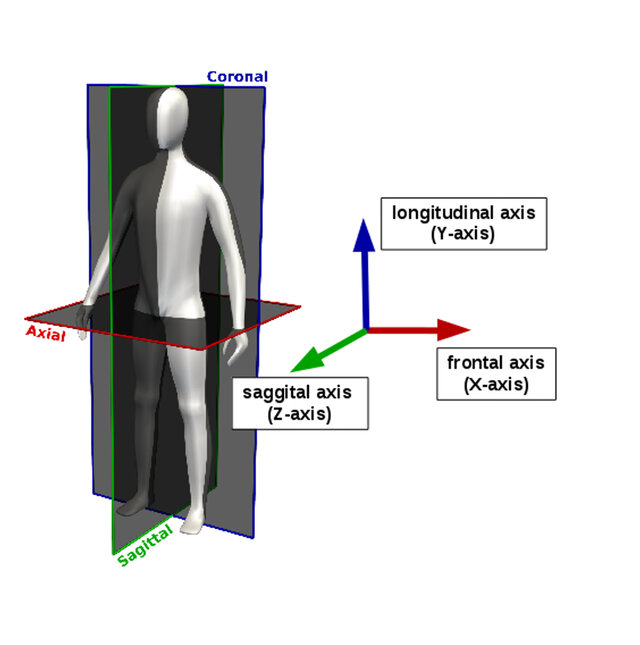
\includegraphics[width=0.7\textwidth]{img/ejes_ct.jpg}
    \caption{Visualización de los planos anatómicos estándar con el sistema de coordenadas correspondiente. Se distinguen tres planos de vista estándar: axial (vista superior), sagital (vista lateral) y coronal (vista frontal). La anatomía se define mediante los siguientes ejes anatómicos: frontal (eje X), longitudinal (eje Y) y sagital (eje Z). Fuente: \cite{heim2018large}}
    \label{fig:ct_ejes_anatomicos}
\end{figure}


En resumen, la TC funciona utilizando rayos X y algoritmos especiales para reconstruir imágenes del interior del cuerpo. A partir de múltiples proyecciones bidimensionales tomadas desde diferentes ángulos, se generan imágenes tridimensionales que permiten ver con detalle la anatomía interna. Estas imágenes pueden visualizarse en cortes axiales, sagitales o coronales, o incluso con técnicas de renderizado más avanzadas que ayudan al diagnóstico médico de forma más precisa.

\section{Descripción general del problema}
La biopsia pulmonar guiada por TC es un procedimiento diagnóstico fundamental para caracterizar lesiones pulmonares y confirmar la presencia de cáncer. Es un paso crucial en el diagnóstico que puede tener un impacto significativo en el resultado para el paciente: 
\begin{itemize}
    \item \textbf{Diagnóstico temprano y mejora de la supervivencia}: el cáncer de pulmón es la causa principal de mortalidad por cáncer y su tasa de supervivencia a 5 años es solo del 18\%, en gran parte debido al diagnóstico en etapas avanzadas \parencite{deng2018clinical}. Por lo tanto, el diagnóstico temprano mediante biopsia es fundamental para mejorar la supervivencia a largo plazo.
    \item \textbf{Confirmación y caracterización}: la biopsia permite obtener muestras de tejido o células para confirmar la presencia de cáncer y determinar sus características específicas, lo cual es esencial para la planificación del tratamiento. Los enfoques para la biopsia de lesiones pulmonares se han desarrollado para proporcionar métodos convenientes y precisos para este diagnóstico.
    \item \textbf{Adaptabilidad a la ubicación de la lesión}: existen diversas técnicas de biopsia que se seleccionan considerando la ubicación y la situación de las lesiones. 
\end{itemize} 

Aunque las biopsias son cruciales para el diagnóstico del cáncer de pulmón, conllevan ciertos riesgos o complicaciones, cuya incidencia puede variar según la técnica utilizada y las características de la lesión. 

En una revisión sistemática de la literatura médica existente realizada por \cite{deng2018clinical}, se encontró con los siguientes resultados tras una biopsia pulmonar transtorácica con aguja guiada por TC (CT-guided PTNB): las dos complicaciones más frecuentes son el neumotórax (acumulación de aire entre el pulmón y la pared torácica) y la hemorragia. Se reportó una incidencia de neumotórax del 22.69\% (946 de 4170 casos) y de hemorragia del 7.08\% (138 de 1949 casos). 
La precisión diagnóstica y la incidencia de complicaciones pueden verse afectadas por el tamaño de la lesión (lesiones más pequeñas pueden disminuir la precisión y aumentar las complicaciones) o la longitud del trayecto de la aguja (trayectos más largos pueden aumentar las complicaciones).


\section{Interés del problema: aplicaciones en medicina}

El interés real de predecir el riesgo de complicaciones en biopsias pulmonares radica en mejorar la seguridad y la calidad del proceso diagnóstico del cáncer de pulmón. Un número considerable de neoplasias pulmonares requiere confirmación histológica mediante biopsia, a menudo guiada por TC. Aunque se trata de un procedimiento generalmente seguro, no está exento de complicaciones relevantes, siendo el neumotórax y la hemorragia pulmonar las más frecuentes.

Actualmente, la estimación del riesgo previo a la biopsia depende en gran medida de la experiencia del médico y de factores clínicos generales como la edad, el historial del paciente o el tamaño y la localización de la lesión. Sin embargo, estos criterios resultan limitados y no permiten una evaluación cuantitativa y personalizada del riesgo. No existen herramientas clínicas que ofrezcan una predicción fiable y objetiva antes de la realización del procedimiento, lo que deja un margen importante para la mejora.

En este contexto, surge la oportunidad de aplicar técnicas de inteligencia artificial y deep learning para desarrollar un sistema predictivo capaz de anticipar complicaciones antes de la biopsia. Este enfoque innovador permitiría abordar el problema como una tarea de clasificación binaria: predecir si un paciente desarrollará complicaciones o no, a partir de datos clínicos tabulares e imágenes médicas tridimensionales. La IA puede detectar patrones sutiles en las características radiómicas de las imágenes, como la textura o la densidad del tejido, imperceptibles para el ojo humano pero potencialmente asociados a un mayor riesgo de complicación.

El desarrollo de una herramienta de este tipo tendría aplicaciones clínicas directas y muy relevantes. Podría integrarse en los sistemas de visualización radiológica para ofrecer al especialista una estimación cuantitativa del riesgo al seleccionar la lesión de interés. Esto facilitaría una toma de decisiones más informada, permitiendo:

\begin{itemize}
    \item Identificar a los pacientes con mayor riesgo de complicaciones.
    \item Adaptar la técnica de biopsia o planificar precauciones adicionales.
    \item Optimizar los recursos sanitarios, por ejemplo, planificando disponibilidad de sangre o material específico si se anticipa un riesgo elevado de hemorragia.
    \item Plantear estrategias diagnósticas alternativas en casos seleccionados.
\end{itemize}

En última instancia, esta herramienta contribuiría a reducir la incidencia de efectos adversos y mejorar la seguridad del paciente, permitiendo además personalizar el procedimiento en función de factores de riesgo conocidos como la presencia de enfisema pulmonar, lesiones de pequeño tamaño o muy próximas a la pleura, o signos radiológicos de hipertensión pulmonar.

En particular, cabe destacar que actualmente no existen investigaciones o literatura científica que aborden de forma específica la predicción del riesgo de complicaciones en biopsias pulmonares mediante técnicas de inteligencia artificial. Esta falta de estudios previos subraya el carácter novedoso de este problema y añade un reto significativo al desarrollo del proyecto. Implica la necesidad de explorar enfoques metodológicos sin referentes establecidos, diseñar estrategias de preprocesamiento y modelado desde cero, y validar cuidadosamente la utilidad clínica de los modelos desarrollados. Este vacío en la investigación hace que la presente propuesta no solo sea innovadora, sino también especialmente relevante para abrir nuevas líneas de trabajo en la aplicación de la IA al apoyo a la decisión médica en procedimientos invasivos.



\section{Descripción de los datos}
La base de datos utilizada en este estudio está formada por un total de 125 pacientes, recopilados de forma progresiva gracias a la colaboración con el Hospital Universitario Clínico San Cecilio de Granada. El primer lote de datos se recibió el 6 de diciembre de 2024, con información de 30 pacientes. A partir de entonces, se fueron incorporando nuevos casos aproximadamente entre dos semanas y un mes, hasta alcanzar los 125 pacientes el 1 de julio. Para cada paciente se dispone de una TC, que constituye un volumen tridimensional. En la mayoría de los casos, estos estudios están centrados en la región pulmonar, aunque algunos incluyen exploraciones de cuerpo entero.
La base de datos se encuentra totalmente anonimizada, cumpliendo con todas las normativas de privacidad y protección de datos personales. 

Los volúmenes 3D presentan variabilidad en sus dimensiones y en el número de cortes o slices ya que el propio hospital tiene diferentes máquinas para hacer las TC. Aunque se ha realizado un preprocesado para ajustar ciertas características, existe heterogeneidad en cuanto al tamaño original de las imágenes, lo cual se gestiona en la fase de preprocesamiento mediante técnicas de normalización y ajuste de tamaño para homogenizar los datos de entrada. En la Figura \ref{fig:ejemplos_planos256x512-label} tenemos un ejemplo de un volúmen desde los tres planos anatómicos. 

Las características de los volúmenes son las siguientes:
\begin{itemize}
    \item \textbf{Número de datos}: 125 pacientes.
    \item \textbf{Tamaño de los datos}: (768,768,x) o (512,512,x) donde la x es el número de slices que varía en cada volumen. 
    \item \textbf{Formato original}: DICOM.
\end{itemize}


\begin{figure}[!htbp]
    \centering
    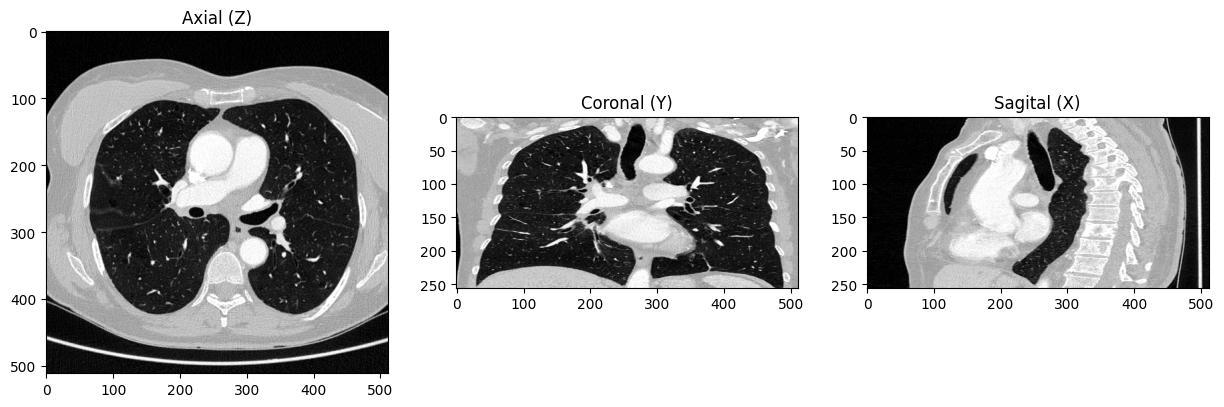
\includegraphics[width=1\textwidth]{img/ejemplos_planos256x512.png}
    \caption{Visualización de un volumen 3D de tamaños (256,512,512) desde los tres planos anatómicos: axial, coronal y sagital. Elaboración propia.}
    \label{fig:ejemplos_planos256x512-label}
\end{figure}

A parte de los volúmenes 3D, disponemos un fichero de datos con datos clínicos tabulares sobre los pacientes. Estos datos incluyen características demográficas, factores de riesgo, información sobre el diagnóstico y evolución de la enfermedad, así como detalles de mutaciones genéticas. La estructura de los datos tabulares es la siguiente: 
\begin{itemize}
    \item \textbf{Paciente}: Identificador anónimo del paciente.
    \item \textbf{Sexo y Edad}: Información demográfica del paciente.
    \item \textbf{Tipo de Cáncer}: Clasificación del tumor pulmonar.
    \item \textbf{Complicación}: Indicación de si el paciente presentó alguna complicación relacionada.
    \item \textbf{Tipo de Complicación}: Especificación de la complicación, en caso de existir.
    \item \textbf{Factor de Riesgo}: Hábitos o condiciones previas del paciente que pueden influir en el diagnóstico (tabaquismo, alcoholismo, obesidad, HTA, DM...).
    \item \textbf{Patología Pulmonar}: Presencia de otras patologías pulmonares adicionales (enfisema paraseptal, enfisema centrolobulillar, fibrosis, neumonía...).
    \item \textbf{Extensión al Diagnóstico}: Evaluación inicial de la extensión del cáncer.
    \item \textbf{TC}: Tipo de dispositivo utilizado para la adquisición de las imágenes de tomografía (Philips B, GE Optima, Philips I, Siemens S...). 
    \item \textbf{Extensión a los 5 años}: Información sobre la progresión del cáncer a largo plazo.
    \item \textbf{Mutación}: Presencia de mutaciones genéticas relevantes en el diagnóstico (p40, p63, CK5/6, CK7...).
\end{itemize}

De todas estas características solo vamos a utilizar las que conocemos antes de hacer la biopsia. Estas variables son: sexo, edad, factor de riesgo y patología pulmonar. Todas las demás características las sabemos una vez realizada la biopsia, por lo que no sirven para la inferencia. La etiqueta a predecir será complicación si estamos ante clasificación binaria o bien tipo de complicación si estamos ante clasificación multietiqueta, ya que se pueden dar varias complicaciones a la vez en un mismo paciente. 

El identificador del paciente es una codificación de los datos más relevantes del mismo:

\begin{itemize}
    \item \textbf{Número de dato:} entero.
    \item \textbf{Sexo:} Mujer (M) u Hombre (H).
    \item \textbf{Tipo de cáncer:} Adenocarcinoma (A), Epidermoide (E), Linfoma de Hodgkin (H), No tumor: posible TBC (T), Linfoma T (L)...
    \item \textbf{Complicación:} Sí o No.
    \item \textbf{Tipo de complicación:} X si no hay complicación y, en caso contrario, se especifica (Hemorragia leve, Neumotórax, Leve derrame pleural...).
\end{itemize}

Por ejemplo, el identificador \textit{1MASh} indica que es el primer paciente de la base de datos, es mujer, tiene adenocarcinoma y ha tenido complicación la cual es hemorragia.

Estos datos clínicos y de imagen se integrarán en el proceso de preprocesamiento y modelado para extraer características relevantes y realizar predicciones diagnósticas. En la siguiente sección se detallarán las transformaciones y selecciones aplicadas sobre esta información para su uso en modelos de aprendizaje automático y profundo.

\subsection{Formato de los datos}
A lo largo de toda esta investigación, se han utilizado diferentes formatos de datos para almacenar y procesar la información. Los volúmenes originales estaban en formato DICOM, que es el estándar para imágenes médicas, y se han convertido a NIfTI para facilitar su manipulación en entornos de análisis de datos. Además, se han utilizado archivos en formato npy para entrenar los modelos.

\paragraph{DICOM}
El formato DICOM (Digital Imaging and Communication in Medicine) se desarrolló para facilitar el intercambio de manera independiente del fabricante del equipo. Además de almacenar las propias imágenes, DICOM  \texttt{.dcm} incluye metadatos relevantes que describen cada estudio, lo que mejora la organización y la interpretación de la información. Gracias a ello, permite un intercambio de datos rápido y seguro, evitando confusiones y errores que podrían surgir al gestionar múltiples archivos para un mismo estudio \parencite{mustra2008overview}.

No solo es un formato de archivo, sino también un protocolo de comunicación de red. Es decir, un archivo DICOM, además de soportar los datos de la imagen, también contiene otra información útil para describirla. Esta información adicional (metadatos), como la descripción del objeto, datos del paciente, procedimientos realizados o informes, y detalles técnicos del dispositivo de imagen (p. ej., fabricante, número de serie, tiempo de exposición para mamografía), se almacena en un encabezado (header). El encabezado DICOM es muy completo, específico de la modalidad y auto-descriptivo, lo que permite que el software entienda cómo se produjo la imagen  \parencite{larobina2014medical}. En nuestro proyecto vienen anonimizados, por lo que esta información viene vacía y no nos da ventaja. 


\paragraph{NIfTI}
NIfTI (Neuroimaging Informatics Technology Initiative) es un formato de archivo desarrollado a principios de la década de 2000 con el objetivo de facilitar y reforzar el análisis de post-procesamiento, especialmente en neuroimagen \parencite{larobina2014medical}.

Típicamente, las imágenes NIfTI  \texttt{.nii} se guardan como un único archivo .nii que fusiona el encabezado (metadatos) y los datos de píxeles \parencite{singh2023secure}.

Además, admite una amplia gama de tipos de datos, incluyendo enteros (con y sin signo, de 8 a 64 bits), flotantes (de 32 a 128 bits) y complejos (de 64 a 256 bits), lo que minimiza la necesidad de factores de escala.

\paragraph{npy}
El formato \texttt{.npy} es el formato nativo de NumPy para almacenar arrays multidimensionales de forma eficiente. En este proyecto se ha utilizado para guardar los volúmenes ya preprocesados como matrices NumPy, listos para ser cargados directamente durante el entrenamiento de los modelos. Este formato ofrece ventajas en términos de velocidad de lectura y escritura, simplicidad de estructura (al contener únicamente datos binarios y metainformación mínima sobre el array) y compatibilidad directa con los pipelines de procesamiento en Python. 

En conclusión, de los formatos descritos, DICOM es el estándar más ampliamente utilizado en entornos clínicos. Se le considera el principal formato de todos los departamentos de imágenes médicas y el estándar líder adoptado por los principales proveedores de equipos de diagnóstico. NIfTI, por su parte, es el formato por defecto en la investigación de neuroimagen y se usa para el intercambio de datos de CT \parencite{larobina2014medical}.


\subsection{Legalidad de los datos}
Los datos médicos utilizados en este proyecto corresponden a volúmenes de TC en formato DICOM que han sido previamente anonimizados realizado por el equipo clínico responsable, eliminando todos los identificadores personales directos e indirectos presentes en los metadatos de los archivos DICOM, conforme a las directrices establecidas en el \emph{Considerando 26 del Reglamento (UE) 2016/679 (RGPD)} \parencite{gdprRecital26}, que estipula que los datos anonimizados de manera irreversible quedan fuera del ámbito de aplicación del RGPD.

En consecuencia, y de acuerdo con lo establecido en la \emph{Ley Orgánica 3/2018}, de \emph{Protección de Datos Personales y garantía de los derechos digitales}, concretamente en su \emph{Disposición adicional decimoséptima, apartado 2, letra e} \parencite{lopd2018}, se considera que no existe ninguna probabilidad razonable de reidentificación de los sujetos a partir de los datos empleados en este estudio. De este modo, se garantiza el pleno cumplimiento de la normativa vigente en materia de protección de datos personales, en línea con las recomendaciones y criterios establecidos por la \emph{Agencia Española de Protección de Datos (AEPD)} \parencite{aepdAnonimizacion}.

Esta garantía de anonimización y cumplimiento normativo es esencial para el desarrollo responsable de proyectos de IA en el ámbito médico, asegurando la protección de la privacidad de los pacientes y el respeto a sus derechos fundamentales.


\section{Dificultades del problema}
El problema de la predicción de complicaciones en biopsias pulmonares mediante inteligencia artificial y técnicas de radiómica representa un desafío considerable en el ámbito de la investigación médica. A diferencia de otras aplicaciones de la IA en medicina, donde se han realizado progresos significativos en la predicción de diagnóstico y clasificación de tumores, la predicción de riesgos asociados a procedimientos invasivos, como la biopsia pulmonar, es un campo aún inexplorado. Actualmente, no existe literatura científica relevante que aborde este problema de forma directa, lo cual evidencia la novedad y la dificultad de esta línea de investigación. Esta falta de estudios previos dificulta la identificación de enfoques metodológicos exitosos y obliga a explorar múltiples técnicas y configuraciones para evaluar su efectividad. Además, la falta de referencias previas introduce un grado de incertidumbre adicional, ya que ni siquiera se tiene la certeza de que esta línea de trabajo sea abordable; es decir, no se sabe si los datos presentan indicios suficientes para identificar patrones y poder predecir los riesgos de manera fiable y precisa.

Una de las principales dificultades encontradas es la disponibilidad de datos. En el ámbito clínico, los datos son limitados y su obtención depende del ritmo de trabajo en los centros hospitalarios. En este trabajo, la recopilación de nuestros datos se realiza exclusivamente en el Hospital Universitario Clínico San Cecilio. De Internet solo se han utilizado datasets para realizar el preentrenamiento en tareas similares, ya que no existen bases de datos públicas con etiquetas específicas de complicaciones en biopsias pulmonares por ser un tema de investigación nuevo en la literatura. Esta restricción impone un límite al volumen de datos disponibles, lo cual dificulta el entrenamiento de modelos de machine learning robustos. Además, los datos tienden a estar desbalanceados, ya que las complicaciones graves son eventos poco frecuentes. Este desbalance entre clases introduce dificultades adicionales en el proceso de entrenamiento, dado que los algoritmos tienden a sobreajustarse a la clase mayoritaria, perdiendo capacidad de generalización para detectar correctamente los eventos adversos.

Adicionalmente, la complejidad del problema se incrementa debido a la naturaleza del propio procedimiento. A diferencia de la detección de tumores en imágenes, donde se buscan anomalías estructurales evidentes, la predicción de complicaciones implica identificar patrones sutiles en la textura, densidad y estructura del tejido pulmonar que puedan estar relacionados con un mayor riesgo. Estos patrones no siempre son evidentes y su detección precisa requiere modelos complejos y técnicas avanzadas de extracción de características.

Por último, cabe destacar el reto de la interpretabilidad. En el ámbito médico, la capacidad de explicar las decisiones tomadas por un modelo predictivo es fundamental para su aceptación clínica. Sin embargo, los modelos de deep learning, que son los que han demostrado mayor capacidad predictiva en tareas relacionadas con imágenes, suelen actuar como cajas negras, dificultando la justificación de sus predicciones. Esta falta de interpretabilidad añade una barrera más en la adopción de estas tecnologías para la toma de decisiones clínicas. 

\section{Metodología}

La metodología de trabajo se enmarca en un enfoque empírico orientado a resolver un problema aplicado en la intersección de la ingeniería informática y la medicina. Se han empleado herramientas y técnicas de deep learning para procesar y analizar volúmenes de TC con el objetivo de predecir complicaciones asociadas a biopsias pulmonares, trabajando con datos reales anonimizados cedidos por el Hospital Universitario Clínico San Cecilio de Granada.

Además, el desarrollo de este trabajo se ha realizado siguiendo un método de trabajo estructurado e inspirado en el método científico, adaptado al problema de predicción del riesgo de complicaciones en biopsias pulmonares mediante técnicas de deep learning:

\begin{itemize}
    \item \textbf{Observación.} Estudio del estado del arte en predicción de complicaciones médicas y en el uso de modelos de deep learning para análisis de imagen médica, especialmente en tomografía computarizada pulmonar. Identificación de la ausencia de estudios específicos para predecir el riesgo en biopsias pulmonares, y análisis de la importancia clínica de este problema.
    
    \item \textbf{Formulación de hipótesis.} Planteamiento de la hipótesis de que es posible predecir el riesgo de complicaciones en biopsias pulmonares a partir de datos clínicos tabulares y volúmenes 3D de TC procesados, empleando modelos de deep learning y aprendizaje automático clásico.
    
    \item \textbf{Recogida de datos.} Recolección progresiva de datos anonimizados en colaboración con el Hospital Universitario Clínico San Cecilio de Granada, incluyendo volúmenes DICOM de TC y variables clínicas asociadas a cada paciente. 
    
    \item \textbf{Preprocesamiento y segmentación.} Diseño de pipelines de preprocesamiento avanzados para normalizar intensidades, ajustar tamaños volumétricos y generar representaciones multiventana. Implementación de segmentación automática del pulmón para restringir el área de análisis del modelo a la región anatómicamente relevante.
    
    \item \textbf{Prueba de hipótesis.} Entrenamiento de modelos de deep learning sobre los datos preprocesados, comparando distintos enfoques (con y sin segmentación, diferentes arquitecturas y configuraciones) para evaluar la capacidad predictiva sobre el riesgo de complicaciones.
    
    \item \textbf{Comprobación y análisis.} Evaluación de los resultados obtenidos mediante métricas específicas de clasificación, matrices de confusión, y comparación con expectativas clínicas. Identificación de limitaciones, discusión de resultados y valoración del potencial clínico real del modelo.
    
    \item \textbf{Conclusiones.} Extracción de conclusiones sobre la viabilidad del enfoque propuesto, la importancia de un preprocesamiento cuidadoso (especialmente la segmentación pulmonar), y la necesidad de futuras líneas de investigación para validar y mejorar los resultados en entornos clínicos reales.
\end{itemize}


\subsection{Software}
El desarrollo del código se ha realizado en \texttt{Python 3.12.7}, un lenguaje flexible y ampliamente utilizado en Inteligencia Artificial \parencite{python}. Para la implementación de los modelos de deep learning se ha empleado \texttt{PyTorch 2.5.1}, una librería de código abierto que facilita el trabajo con redes neuronales y permite el uso eficiente de GPUs  (\emph{Graphics Processing Units}, unidades de procesamiento de gráficos) para acelerar las operaciones sobre tensores \parencite{paszke2019pytorch}.

En el proyecto también ha sido utilizado \texttt{MONAI} (Medical Open Network for Artificial Intelligence), concretamente la versión 1.4.0, un framework basado en PyTorch especializado en imagen médica \parencite{cardoso2022monai}. MONAI ha permitido diseñar pipelines de preprocesamiento avanzados y consistentes para volúmenes 3D, incluyendo transformaciones personalizadas como \texttt{Windowingd} y \texttt{MultiWindowingd} para la normalización de intensidades en unidades Hounsfield, así como técnicas de data augmentation en 3D con \texttt{RandAffined}. Se definieron diferentes pipelines para entrenamiento y validación, integrando resize trilineal a un tamaño fijo, normalización, generación de canales multiventana y conversiones a tensores. También se implementaron transformaciones para combinar máscaras segmentadas con las imágenes de entrada, utilizando estrategias como enmascarado o apilado de canales.

Además, se desarrolló un módulo de segmentación automática basado en la herramienta \texttt{TotalSegmentator}, que permitió generar de forma sistemática las máscaras pulmonares a partir de volúmenes TC originales \parencite{wasserthal2023totalsegmentator}. Este paso fue clave para restringir la atención del modelo únicamente al pulmón, evitando que aprendiera correlaciones insignificantes de regiones fuera del área de interés clínico. El script de segmentación automatiza la conversión de lotes de archivos NIfTI en máscaras segmentadas, con soporte para ejecución en GPU o CPU.

Se han diseñado utilidades específicas para el particionado del dataset, permitiendo la generación de splits de entrenamiento, validación y test de forma reproducible y estratificada. Esto incluyó soporte para divisiones simples y k-fold cross-validation, asegurando el equilibrio de clases en cada partición. Todo el sistema de organización de datos se estructuró para mantener trazabilidad y facilitar la reutilización en distintos experimentos.

Para el manejo de datos médicos se utilizó \texttt{NiBabel} (lectura y escritura de archivos NIfTI) \parencite{nibabel}, \texttt{NumPy} para operaciones matriciales \parencite{harris2020array} y \texttt{Matplotlib} para visualizaciones 2D y 3D de imágenes \parencite{Hunter:2007}, segmentaciones y resultados intermedios del preprocesamiento. Para el manejo de tablas y datos clínicos tabulares se empleó \texttt{Pandas} \parencite{mckinney-proc-scipy-2010}, y para la extracción de características radiómicas a partir de volúmenes médicos se utilizó la librería \texttt{PyRadiomics} \parencite{van2017computational}. La fase de desarrollo y pruebas se realizó utilizando \texttt{Visual Studio Code} como editor principal \parencite{vscode}, junto con \texttt{Jupyter Notebooks} para análisis exploratorio, transformaciones y visualización interactiva de resultados \parencite{jupyter}. También han sido utilizadas las librerías \texttt{scikit-learn 1.5.2} \parencite{scikit-learn} y \texttt{scikit-image 0.25.0} para otras utilidades \parencite{van2014scikit}.

Además, en todo momento se ha utilizado el programa \texttt{3D Slicer} para controlar la visualización, procesamiento, segmentación y análisis de los volúmenes 3D \parencite{pieper20043d}. 

Todo el código desarrollado se encuentra disponible en el siguiente repositorio de GitHub: \url{https://github.com/mcribi/TFG}.

\subsection{Hardware}

En cuanto al hardware, el desarrollo inicial se realizó en un portátil personal Victus by HP Gaming Laptop 16-r0xxx las siguientes especificaciones: 

\begin{itemize}
    \item \textbf{Procesador (CPU)}: 13th Gen Intel® Core™ i7-13620H a 4.9 GHz.
    \item \textbf{Memoria RAM}: 32 GB.
\end{itemize}

Para las tareas de entrenamiento y evaluación de modelos se emplearon los servidores de cómputo de alto rendimiento (NGPU) proporcionados por la Universidad de Granada (UGR) cuyas máquinas se encuentran ubicadas en CPD Santa Lucía. 

La infraestructura NGPU de la UGR cuenta con un clúster de nodos de cómputo que incluyen diversas configuraciones de GPUs como GTX Titan, X Pascal, GTX Titan Xp, RTX 2080 Ti, Titan RTX, Tesla V100 (32GB) y Tesla A100 (40GB). Estas han permitido entrenar tanto modelos 2D como 3D.


\section{Técnicas para abordar el problema}
A continuación se describen de forma general todas las técnicas y estrategias empleadas a lo largo del proyecto, que se explican en mayor detalle en las distintas secciones de esta memoria.

En primer lugar, se realizó un análisis exploratorio de datos (EDA) exhaustivo, que incluyó la \textit{visualización de gráficas} y el \textit{análisis estadístico} de variables tanto clínicas como de imagen. Este paso fue clave para comprender la distribución de los datos, identificar posibles sesgos y diseñar las estrategias de preprocesamiento más adecuadas.

El preprocesamiento de los datos jugó un papel esencial. En el caso de las imágenes médicas en TC, se aplicaron \textit{ventanas de Hounsfield} para normalizar intensidades en rangos clínicamente relevantes, y se incorporó un paso de \textit{segmentación pulmonar} mediante la herramienta TotalSegmentator, con el objetivo de centrar el análisis exclusivamente en el pulmón. También se realizaron procesos de \textit{limpieza de ortografía} y unificación en las variables clínicas, \textit{eliminación de columnas irrelevantes}, \textit{normalización} de variables numéricas y \textit{binarización} de variables multietiqueta. Para los volúmenes 3D se implementaron \textit{transformaciones} como el \textit{windowing multicanal} y la \textit{interpolación trilineal} para ajustar los datos a diferentes tamaños estándar ((256,512,512), (128,256,256), (64,64,64), (28,28,28), (128,128,128)), permitiendo así su uso en redes convolucionales con diferentes capacidades y restricciones de memoria. Además, se aplicaron técnicas de \textit{data augmentation} para mejorar la capacidad de generalización de los modelos.

En el caso de los modelos 2D, se utilizaron arquitecturas basadas en \textit{EfficientNetV2-S} con pesos preentrenados en ImageNet1\_v1, aplicando técnicas de \textit{fine-tuning} con congelación de capas. El entrenamiento incluyó \textit{validación cruzada} (5-fold simple, 5-fold estratificada, 5-fold estratificada por paciente) y enfoques \textit{leave-one-out}. Para mejorar el entrenamiento se incorporaron técnicas como el \textit{EarlyStopping} y se empleó la función de pérdida binaria (\textit{BCE Loss}).

Para los modelos 3D se trabajó principalmente con \textit{DenseNet121} y \textit{ResNet} adaptados a volúmenes tridimensionales. Se exploraron diferentes funciones de pérdida como \textit{CrossEntropyLoss} (incluyendo variantes ponderadas con \textit{class weights} calculados según la distribución de clases) y \textit{Focal Loss} para abordar el desbalanceo. También se empleó el \textit{WeightedRandomSampler} con distintos exponente de ponderación para ajustar la probabilidad de muestreo de las clases minoritarias. Se trató el desbalanceo ya que, aunque en el total de datos recogidos no hay un gran desbalanceo, en fechas anteriores sí existía un gran desbalanceo hacia la no complicación. El optimizador principal fue \textit{AdamW}, acompañado del scheduler \textit{ReduceLROnPlateau} para el ajuste dinámico del learning rate y otros programas. Para mitigar el problema de memoria (out of memory) al trabajar con volúmenes grandes y batch sizes pequeños, se implementó \textit{acumulación de gradiente} para simular batch sizes mayores. Asimismo, se aplicaron técnicas de data augmentation específicas para la clase minoritaria mediante transformaciones como \textit{RandFlip}, \textit{RandRotate90d}, \textit{RandZoomd} y \textit{RandGaussianNoise}. El entrenamiento se complementó con técnicas de explicabilidad como \textit{Grad-CAM}, tanto en 2D como en 3D, para analizar la atención del modelo y validar su interpretabilidad clínica.

También se exploró el uso de un \textit{dataset genérico} de CT pulmonar disponible públicamente, con el objetivo de evaluar la viabilidad del problema y la capacidad de los modelos para predecir el tipo de cáncer. Este conjunto de datos se preprocesó de forma equivalente y se entrenó con modelos 3D (DenseNet121), aplicando técnicas de explicabilidad y funciones de pérdida adaptadas al fuerte desbalanceo entre clases. 

Finalmente, se aplicaron técnicas de \textit{aprendizaje automático clásico} sobre los datos tabulares y sobre \textit{características radiómicas} extraídas de las imágenes mediante \textit{PyRadiomics}, entrenando modelos con distintos hiperparámetros y aplicando estrategias de balanceo como SMOTE para mitigar el desequilibrio de clases.



\section{Presupuesto}

A continuación, se presenta el presupuesto estimado para la realización del proyecto \textit{Predicción de Complicaciones en Biopsias Pulmonares mediante Inteligencia Artificial}. Este presupuesto incluye los recursos humanos necesarios para el desarrollo del proyecto, la capacidad de cómputo para el entrenamiento y validación de los modelos predictivos, así como otros servicios adicionales requeridos. La duración total del proyecto se estima en \textit{8 meses}, de diciembre del 2024 a julio del 2025. 

Se excluyen de este presupuesto los costes personales propios del investigador, como el uso de un ordenador portátil, el alquiler de vivienda o el consumo eléctrico doméstico.

Las fuentes para la estimación de costes son \textit{Glassdoor} \footnote{\url{https://www.glassdoor.es/Sueldos/junior-software-engineer-sueldo-SRCH_KO0\%2C24.htm}}, \textit{SalaryExpert} \footnote{\url{https://www.salaryexpert.com/salary}} y \textit{Google Cloud} \footnote{\url{https://cloud.google.com/compute/gpus-pricing}} respectivamente.

\subsection{Recursos Humanos}

El equipo del proyecto está compuesto por el investigador principal (responsable del desarrollo y análisis de modelos de predicción), un médico colaborador (encargado de la validación clínica y supervisión médica de los datos) y el tutor académico que supervisa el trabajo. A continuación, en la Tabla \ref{tab:recursos-humanos}, se detallan los costes asociados.

\begin{table}[!htbp]
    \centering
    \begin{tabular}{|l|c|c|c|}
        \hline
        \textbf{Recurso} & \textbf{Coste Mensual (€)} & \textbf{Duración (meses)} & \textbf{Coste Total (€)} \\ \hline
        Investigador Principal & 1.300 € & 8 & 10.400 € \\ 
        Médico Colaborador    & 2.000 € & 8 & 16.000 € \\ 
        Tutor Académico (25 h) & 2.000 € & 1 & 2.000 € \\ \hline
        \textbf{Total Recursos Humanos} & & & \textbf{28.400 €} \\ \hline
    \end{tabular}
    \caption{Presupuesto destinado a recursos humanos.}
    \label{tab:recursos-humanos}
\end{table}

\subsection{Capacidad de Cómputo}

El desarrollo del modelo predictivo requiere infraestructura de alto rendimiento para procesar imágenes 3D y entrenar redes neuronales. Para ello, se estima el uso de servidores en la nube con GPUs y almacenamiento en la Tabla \ref{tab:computo}.

\begin{table}[!htbp]
    \centering
    \begin{tabular}{|l|c|c|c|}
        \hline
        \textbf{Recurso} & \textbf{Coste Mensual (€)} & \textbf{Duración (meses)} & \textbf{Coste Total (€)} \\ \hline
        Servidores Cloud (GPUs - AWS, GCP) & 100 € & 8 & 800 € \\ 
        Almacenamiento (1 TB en Cloud) & 50 € & 8 & 400 € \\ \hline
        \textbf{Total Capacidad de Cómputo} & & & \textbf{1.200 €} \\ \hline
    \end{tabular}
    \caption{Presupuesto destinado a capacidad de cómputo.}
    \label{tab:computo}
\end{table}

\subsection{Materiales y Otros Gastos}

Para este proyecto no se prevén gastos en licencias de software, ya que todas las herramientas utilizadas son de código abierto y licencia libre (PyTorch, MONAI, PyRadiomics, etc.). Tampoco se consideran necesarias otras compras de materiales o servicios adicionales.

\subsection{Presupuesto Total Estimado}

El presupuesto total estimado para el desarrollo del proyecto durante un periodo de 8 meses asciende a \textbf{29.600 €}, e incluye todos los recursos humanos y la capacidad de cómputo necesarios para su correcta ejecución.


\section{Diario de trabajo}

El desarrollo de este proyecto se ha realizado de forma progresiva a lo largo de varios meses, en estrecha coordinación con el Hospital Universitario Clínico San Cecilio de Granada. Los datos fueron llegando de forma escalonada en distintas entregas, lo que obligó a diseñar un flujo de trabajo adaptable y un preprocesamiento escalable que pudiera incorporar la nueva información conforme se recibía. Las fechas de entrega de los datos fueron las siguientes:

\begin{itemize}
    \item 6 de diciembre de 2024: 30 pacientes.
    \item 30 de enero de 2025: 40 pacientes.
    \item 26 de febrero de 2025: 53 pacientes.
    \item 18 de marzo de 2025: 72 pacientes.
    \item 23 de abril de 2025: 76 pacientes, junto con 100 controles sanos adicionales.
    \item 12 de mayo de 2025: 92 pacientes.
    \item 28 de mayo de 2025: 101 pacientes.
    \item 18 de junio de 2025: 112 pacientes.
    \item 1 de julio de 2025: 125 pacientes en total.
\end{itemize}

Desde diciembre hasta enero incluido, se dedicó tiempo a la revisión de literatura médica relevante para comprender mejor el problema clínico y las variables recogidas por el hospital. Durante este período también se exploraron los programas médicos utilizados y se consolidaron conocimientos de programación en Python aplicados a datos médicos, para sentar las bases del preprocesamiento y análisis posterior.

En febrero, tras este estudio preliminar, se realizó un análisis exhaustivo de las variables tabulares, identificando aquellas relevantes para el entrenamiento y descartando las que no aportaban valor o podían inducir fuga de información. Se desarrolló un análisis exploratorio de datos (EDA) inicial y se comenzó a construir el pipeline de preprocesamiento, con especial atención a su escalabilidad dado que los datos continuarían llegando por lotes. Fue necesario verificar cuidadosamente los datos tabulares e imágenes, ya que se detectaron archivos corruptos que el equipo médico tuvo que reemplazar. Durante esta fase se mantuvieron reuniones con el personal médico para entender de forma cualitativa qué factores clínicos consideran ellos que predicen el riesgo de complicación.

En marzo se experimentó con modelos basados en cortes axiales 2D debido a sus menores requisitos computacionales, pero pronto se comprobó que dividir los volúmenes en slices individuales implicaba una pérdida de información espacial importante. Por ello, se decidió enfocar el desarrollo en modelos 3D completos, ajustando el preprocesamiento tanto para datos 2D como para volúmenes 3D.

Durante abril se trabajó intensamente en abordar el desbalanceo de clases, ya que los datos acumulados hasta esa fecha presentaban una clara predominancia de pacientes sin complicaciones. En este periodo se entrenaron modelos sin segmentación pulmonar, observándose resultados insatisfactorios: las técnicas de explicabilidad mostraban que el modelo se fijaba en regiones ajenas al pulmón. También se probó el preentrenamiento en un dataset público para la predicción del tipo de cáncer pulmonar, pero no se obtuvieron mejoras significativas.

En mayo se incorporó la segmentación pulmonar al pipeline de preprocesamiento, utilizando máscaras generadas con TotalSegmentator para limitar la atención del modelo a la región anatómica relevante. Esta estrategia permitió mejorar los resultados obtenidos. Además, se realizaron los últimos experimentos con modelos 3D, incluyendo nuevas pruebas de preentrenamiento con otro dataset. 

En junio se dedicó por completo a la extracción de características de radiómica y su experimentación.

Finalmente, el mes de julio se dedicó íntegramente a completar y revisar la memoria del trabajo, asegurando la correcta redacción, coherencia y presentación de todos los resultados y conclusiones obtenidas.

Todas estas tareas se pueden agrupar en las siguientes fases:

\begin{itemize}
    \item \textbf{Revisión de la literatura y formación técnica:} estudio de artículos médicos sobre biopsias pulmonares y complicaciones asociadas, revisión de factores de riesgo clínicos y tecnologías de radiómica. Formación en programación en Python aplicada al procesamiento de datos médicos, incluyendo librerías específicas para imágenes 3D.

    \item \textbf{Análisis exploratorio y preprocesamiento:} incluye el análisis y limpieza de datos clínicos, selección de variables relevantes, y exploración de la distribución de las variables y su relación con las complicaciones (EDA). Desarrollo de un diseño modular y escalable para el preprocesamiento, validación manual para corregir errores como archivos corruptos, y generación de máscaras pulmonares con TotalSegmentator para limitar la atención del modelo a la región anatómica relevante.

    \item \textbf{Diseñar modelos:} diseño conceptual del flujo de trabajo de los modelos, definición de la arquitectura base y de las estrategias de integración multimodal (volúmenes TC con datos clínicos), así como consideración de diferentes estrategias para abordar el desbalanceo de clases mediante samplers ponderados o funciones de pérdida adaptadas.

    \item \textbf{Experimentación:} incluye pruebas iniciales con cortes axiales 2D y la posterior transición a modelos 3D completos para preservar la información espacial. Al final, se experimentó con la radiómica. 

    \item \textbf{Fundamentos matemáticos:} estudio de las bases matemáticas para la parte práctica. 

    \item \textbf{Memoria:} redacción progresiva y estructurada de la memoria del TFG a lo largo del proyecto, asegurando la coherencia global, la correcta integración de resultados y el análisis crítico de los mismos.
\end{itemize}


En conjunto, este enfoque permitió mantener una metodología de trabajo estructurada pero flexible, adaptándose a la llegada progresiva de nuevos datos y a los hallazgos intermedios. Además, facilitó la integración de la parte clínica con la informática, asegurando que el resultado final respondiera a una necesidad médica real con una solución técnica sólida y justificada.

Para visualizar el trabajo realizado en estos meses, se muestra un diagrama de Gantt de la planificación en la Figura \ref{fig:gantt_chart}.

\begin{figure}[!htbp]
    \centering
    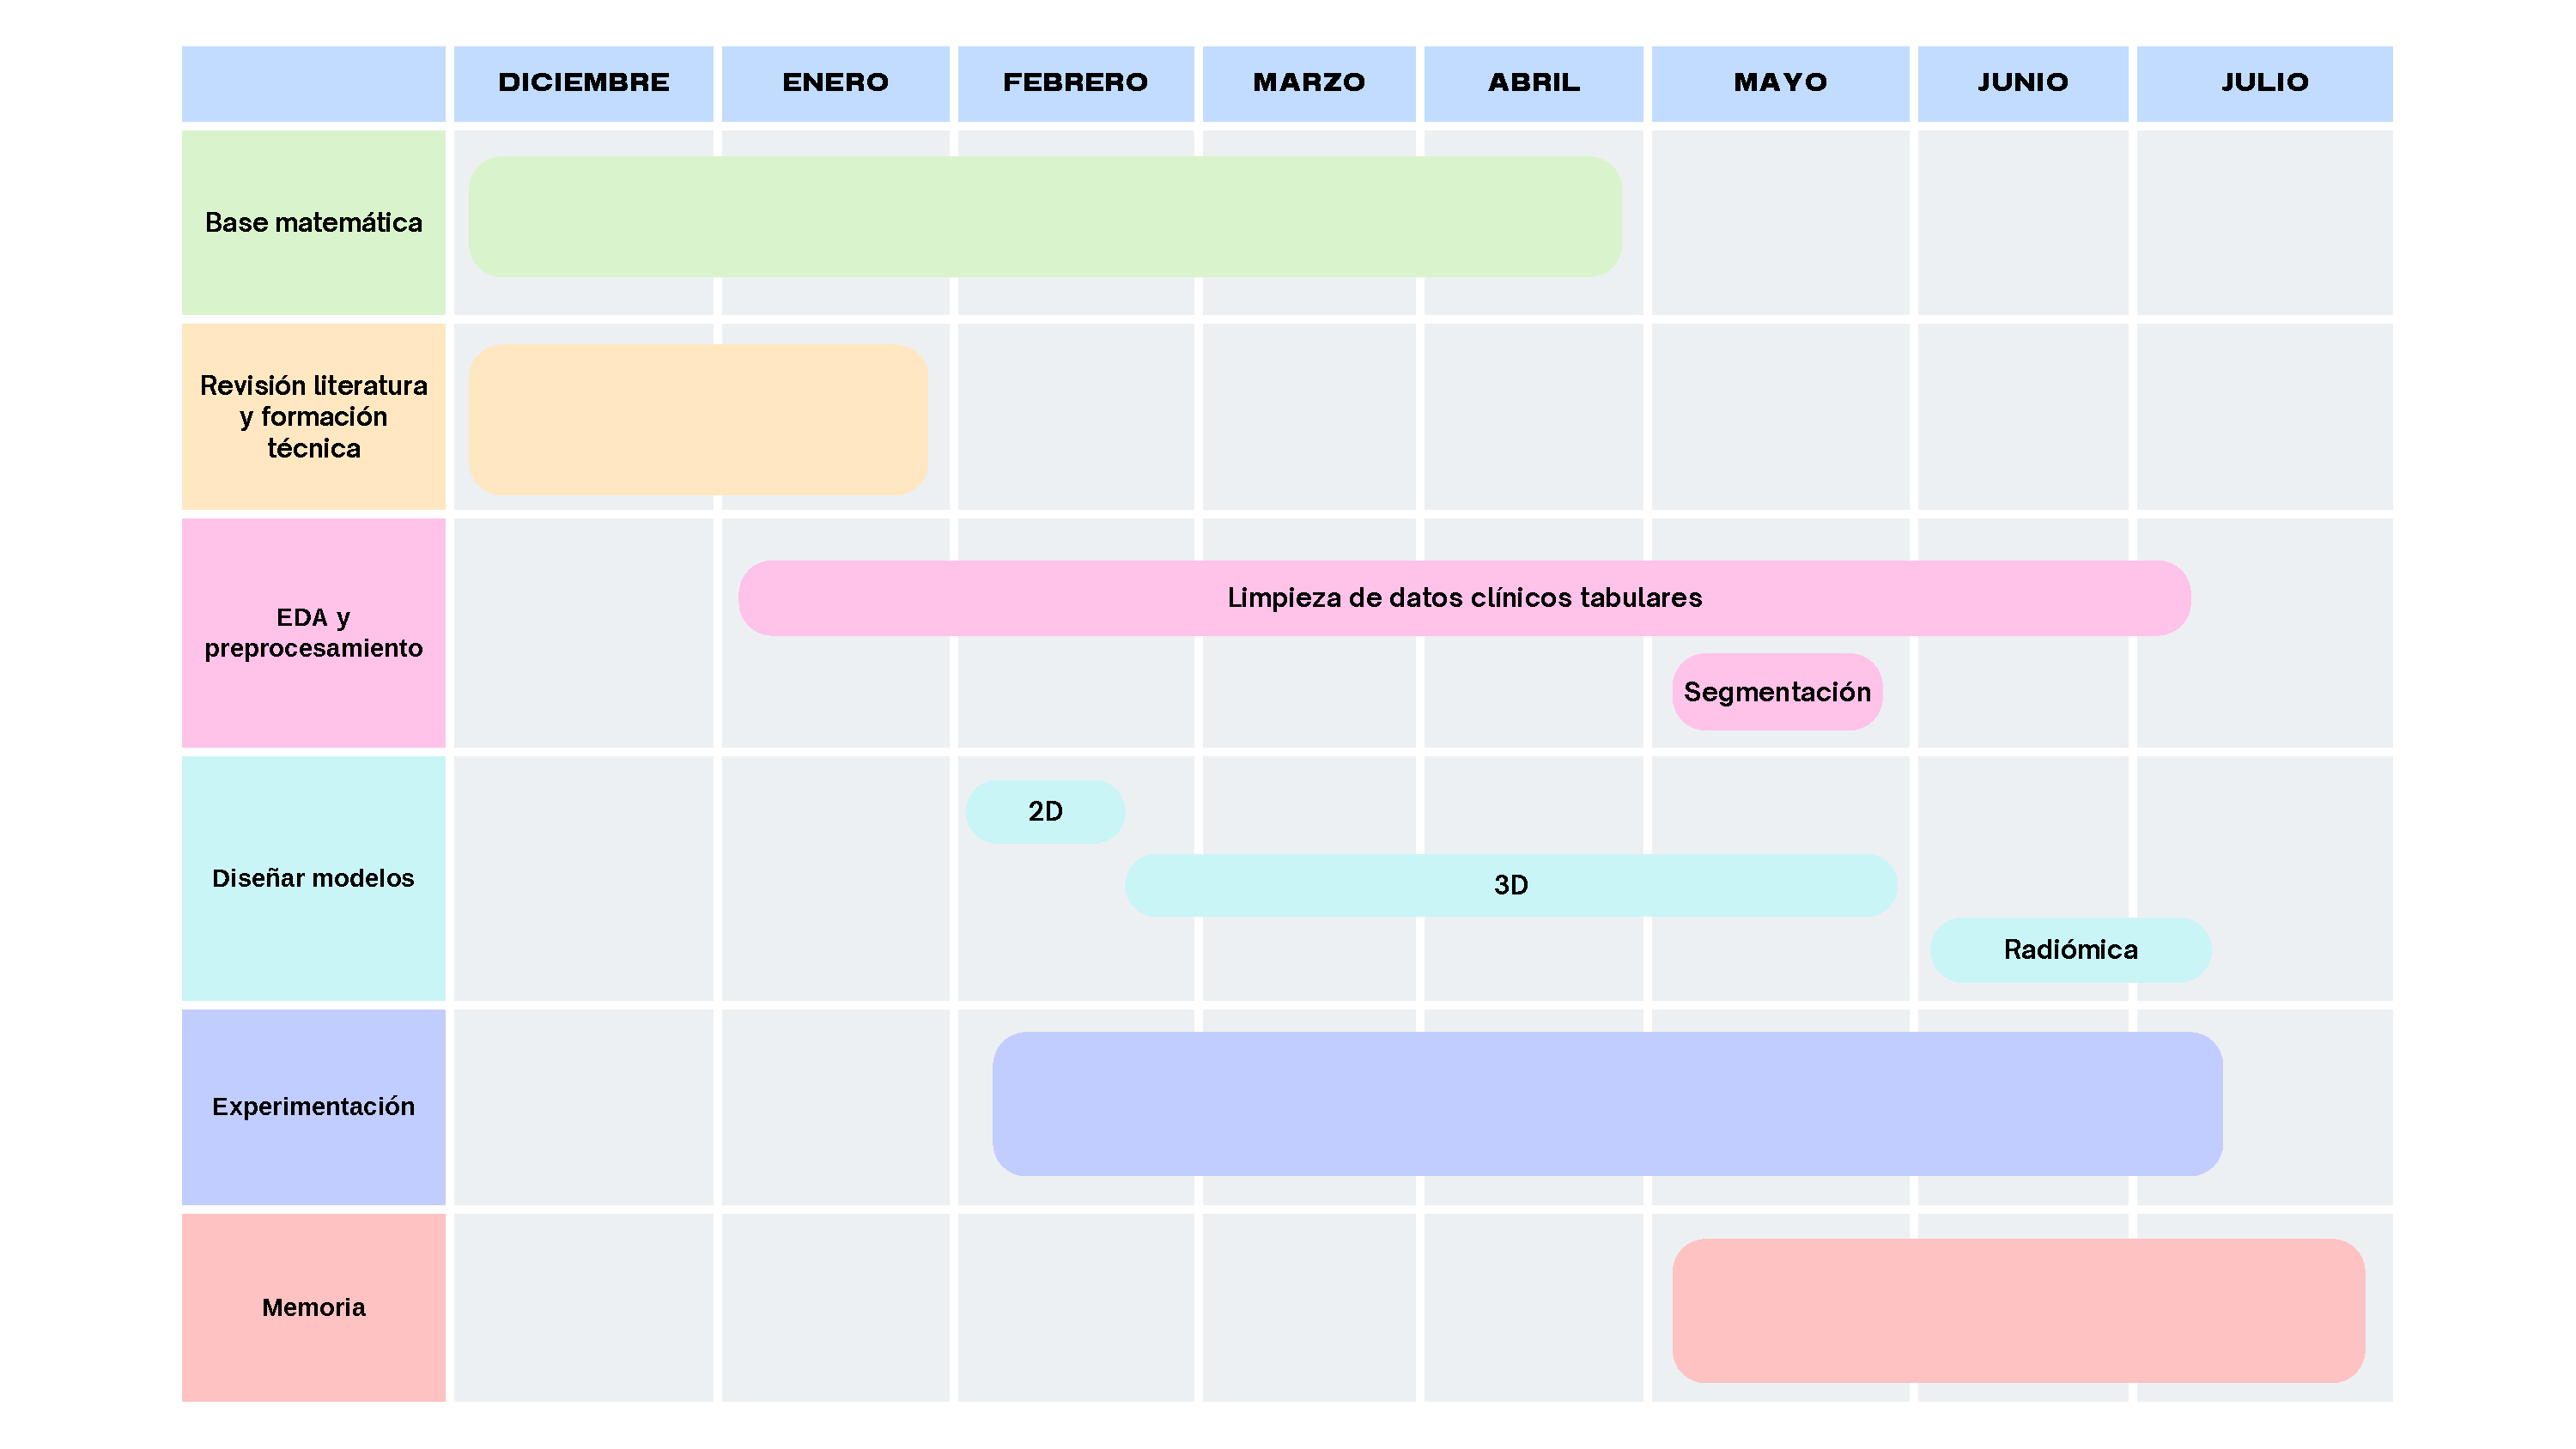
\includegraphics[width=1.1\textwidth]{img/gantt.pdf}
    \caption{Diagrama de Gantt del proyecto}
    \label{fig:gantt_chart}
\end{figure}

\endinput
%--------------------------------------------------------------------
% FIN DEL CAPÍTULO. 
%--------------------------------------------------------------------

% !TeX root = ../tfg.tex
% !TeX encoding = utf8

\chapter{Análisis de datos y preprocesamiento} \label{eda}

En esta sección se presenta el análisis exploratorio de los datos disponibles en el proyecto y el preprocesamiento de los mismos. Se diferencian dos tipos de datos principales: los volúmenes de imagen originales en tipo DICOM y los datos clínicos tabulares. El objetivo de este análisis es entender la estructura, características y potenciales problemas de los datos antes de diseñar el preprocesamiento y los modelos.

% -----------------------------
\section{Análisis de datos}
Empezamos con el análisis de los volúmenes de imagen en formato DICOM, que constituyen la base del dataset.
% -----------------------------
\subsection{Análisis de datos de volúmenes DICOM}
El segundo componente del dataset corresponde a los volúmenes de imagen en formato DICOM. Para su análisis, se recorrieron de forma recursiva las carpetas anonimizadas para contabilizar los archivos correspondientes a cada paciente y extraer características como el número de slices (profundidad del volumen) y la resolución axial (Height y Width).

Para empezar, se generó un histograma para visualizar la distribución del número de slices por volumen. La distribución es claramente asimétrica y presenta un sesgo hacia la derecha, con un pico principal entre aproximadamente 200 y 300 cortes por paciente. Sin embargo, existen casos con más de 900 slices, considerados outliers.


\begin{figure}[!htbp]
    \centering
    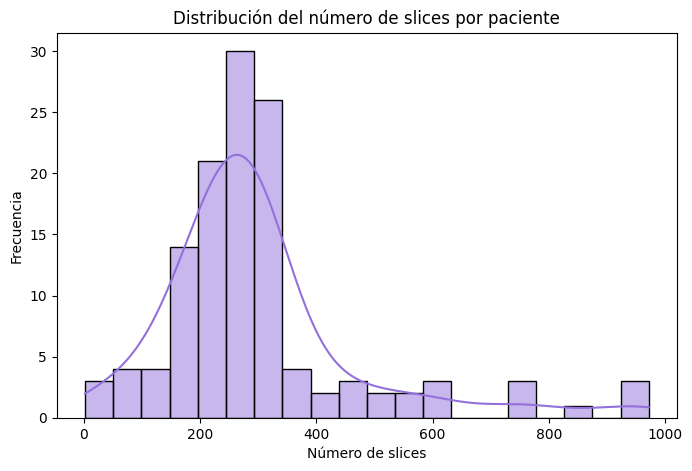
\includegraphics[width=0.7\textwidth]{img/histograma_dist_slices_x_paciente.png}
    \caption{Distribución del número de slices por paciente.}
    \label{fig:distribucion_slices}
\end{figure}

La alta variabilidad mostrada en la Figura \ref{fig:distribucion_slices} en la dimensión axial es importante porque, en modelos de redes convolucionales 3D, la entrada debe tener un tamaño fijo en todas sus dimensiones. Por ello, será necesario aplicar técnicas de preprocesamiento para normalizar este eje, como el recorte central de slices o la interpolación lineal para aumentar el número de cortes en volúmenes más pequeños.


En cuanto a las dimensiones de cada corte (height y width), se han encontrado dos resoluciones:

\begin{itemize}
    \item \textbf{512x512}: presente en 70 volúmenes.
    \item \textbf{768x768}: presente en 55 volúmenes.
\end{itemize}

Esta relativa homogeneidad facilitará el preprocesamiento, permitiendo reescalar todas las imágenes a un tamaño fijo común para garantizar consistencia en los datos de entrada del modelo.


\subsection{Análisis exploratorio de datos clínicos}
El conjunto de datos clínicos contiene información de 125 pacientes, cada uno identificado mediante un código único. En la recopilación original de los datos médicos se incluían las siguientes variables: Identificador del paciente, Sexo, Edad, Tipo de cáncer, Complicación, Tipo de complicación, Factor de riesgo, Patología pulmonar, Extensión al diagnóstico, TC (máquina en la que se realiza la prueba), Extensión a los 5 años y Mutación.

Sin embargo, muchas de estas variables se conocen únicamente tras la biopsia, por lo que su inclusión en el entrenamiento del modelo introduciría un sesgo de información. Por este motivo, se han eliminado las variables \textit{Extensión al diagnóstico}, \textit{TC}, \textit{Extensión a los 5 años} y \textit{Mutación}. Además, aunque el \textit{Tipo de cáncer} se elimina en el preprocesamiento, se ha mantenido su análisis descriptivo dado que proporciona contexto clínico relevante.

Tras este filtrado inicial, las variables de interés para el análisis exploratorio son:

\begin{itemize}
    \item \textbf{Identificador del paciente}: código único para trazabilidad (no usado en entrenamiento).
    \item \textbf{Sexo}: variable categórica binaria (Hombre/Mujer). Se observa un ligero desbalanceo hacia la categoría masculina.
    \item \textbf{Edad}: variable numérica entera. La distribución está centrada en el rango de 65-70 años, destacando la predominancia de pacientes de edad avanzada.
    \item \textbf{Complicación}: variable objetivo binaria (Sí/No). Presenta un leve desbalanceo hacia la ausencia de complicación.
    \item \textbf{Tipo de complicación}: variable categórica multietiqueta (solo para casos positivos).
    \item \textbf{Factor de riesgo}: variable de texto con potencial multietiqueta.
    \item \textbf{Patología pulmonar}: condiciones respiratorias previas. Variable de texto también multietiqueta.
    \item \textbf{Tipo de cáncer}: aunque se elimina en preprocesamiento, se analiza aquí por ser el cáncer de pulmón el principal problema de estudio.
\end{itemize}

Antes de realizar el análisis estadístico, se llevó a cabo un proceso exhaustivo de limpieza, corrigiendo errores de ortografía, unificando conceptos médicos sinónimos y eliminando inconsistencias. Tras la limpieza, se verificó la ausencia de valores nulos.


\begin{figure}[!htbp]
    \centering
    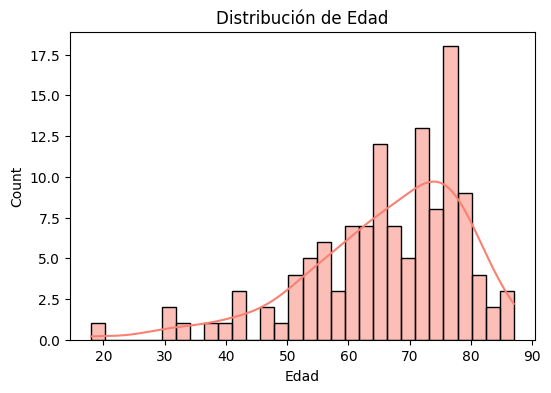
\includegraphics[width=0.65\textwidth]{img/histograma_dist_edad.png}
    \caption{Distribución de la edad de los pacientes.}
    \label{fig:distribucion_edad}
\end{figure}

En el histograma de edad de la Figura \ref{fig:distribucion_edad} se aprecia cómo la mayoría de los pacientes se agrupa en la franja de 65 a 80 años, con muy pocos casos por debajo de los 30 años. Esto refleja que se trata de una población mayor, aspecto importante para la interpretación clínica y la generalización del modelo.


\begin{figure}[!htbp]
    \centering
    \begin{minipage}[b]{0.45\textwidth}
        \centering
        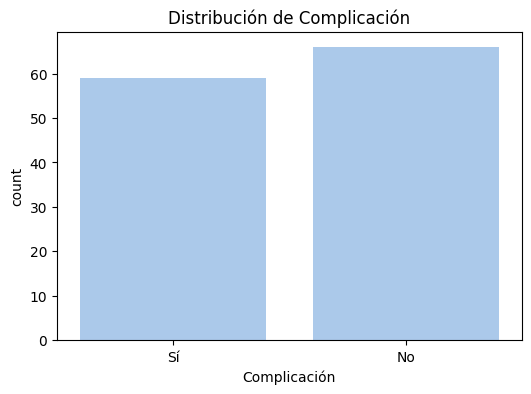
\includegraphics[width=\textwidth]{img/histograma_dist_complicacion.png}
        \caption{Distribución de la variable Complicación (Sí / No).}
        \label{fig:distribucion_complicacion}
    \end{minipage}
    \hspace{0.05\textwidth}
    \begin{minipage}[b]{0.45\textwidth}
        \centering
        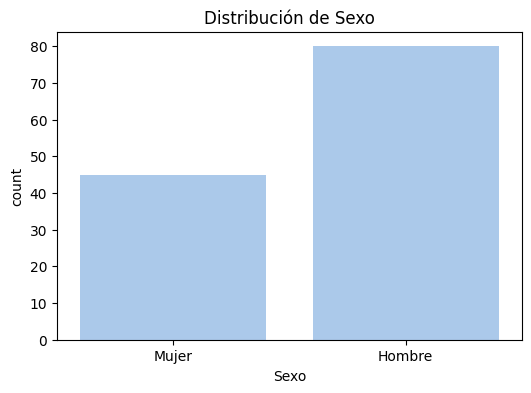
\includegraphics[width=\textwidth]{img/histograma_dist_sexo.png}
        \caption{Distribución de la variable Sexo (Hombre / Mujer).}
        \label{fig:distribucion_sexo}
    \end{minipage}
\end{figure}

La Figura \ref{fig:distribucion_complicacion} muestra que la variable \textit{Complicación} presenta un leve desbalanceo hacia los casos sin complicación, mientras que la Figura \ref{fig:distribucion_sexo} muestra que la variable \textit{Sexo} tiene un predominio masculino. Cabe destacar que el tema del desbalanceo en la variable \textit{Complicación} se estudió especialmente durante las primeras fases del proyecto, ya que con los datos disponibles hasta ese momento el desbalanceo era considerable. Sin embargo, con la llegada de nuevos lotes y la base de datos completa, dicho desbalanceo se redujo significativamente, por lo que no fue necesario aplicar técnicas específicas en las fases finales. Por su parte, el desbalanceo en la variable \textit{Sexo} no ha sido tratado de forma específica.

Como parte del análisis exploratorio, se estudió la distribución de la Figura \ref{fig:distribucion_tipo_cancer} del \textit{Tipo de cáncer}, aunque esta variable se eliminará en el entrenamiento. 

\begin{figure}[!htbp]
    \centering
    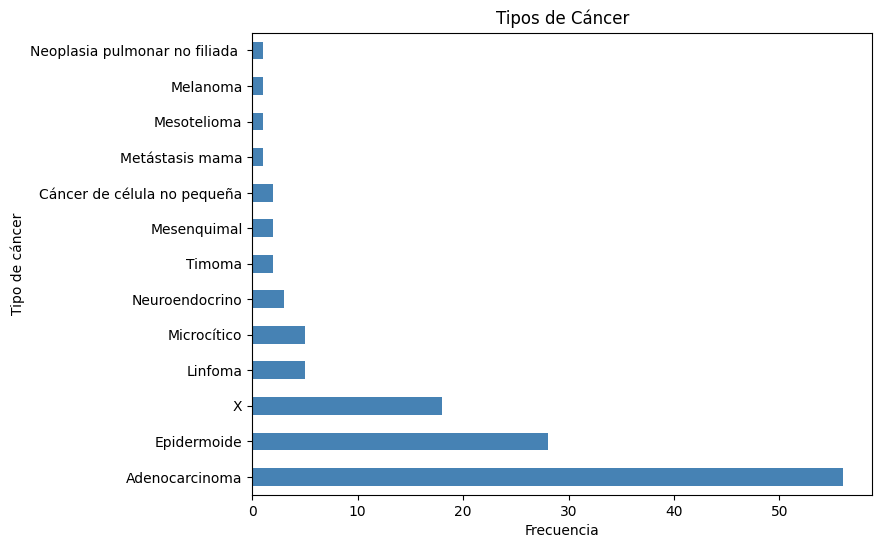
\includegraphics[width=1\textwidth]{img/barras_tipo_cancer.png}
    \caption{Frecuencia de categorías en Tipo de cáncer.}
    \label{fig:distribucion_tipo_cancer}
\end{figure}
 

Para las variables multietiqueta como \textit{Tipo de complicación}, \textit{Factor de riesgo} y \textit{Patología pulmonar} (Figuras  \ref{fig:distribucion_tipo_complicacion}, \ref{fig:distribucion_patologia_pulmonar} y \ref{fig:distribucion_factor_riesgo} respectivamente), se analizaron sus distribuciones para entender la diversidad de categorías presentes en el dataset. 


\begin{figure}[!htbp]
    \centering
    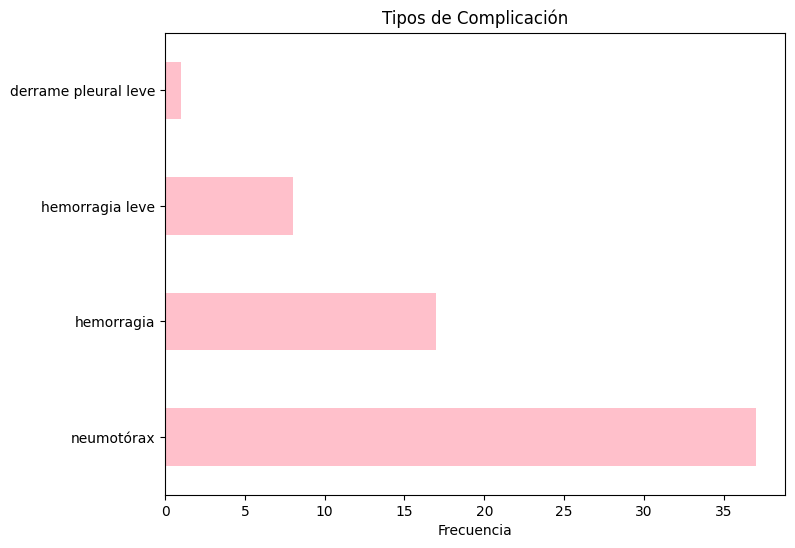
\includegraphics[width=1\textwidth]{img/barras_tipo_complicacion.png}
    \caption{Frecuencia de categorías en Tipo de complicación.}
    \label{fig:distribucion_tipo_complicacion}
\end{figure}


\begin{figure}[!htbp]
    \centering
    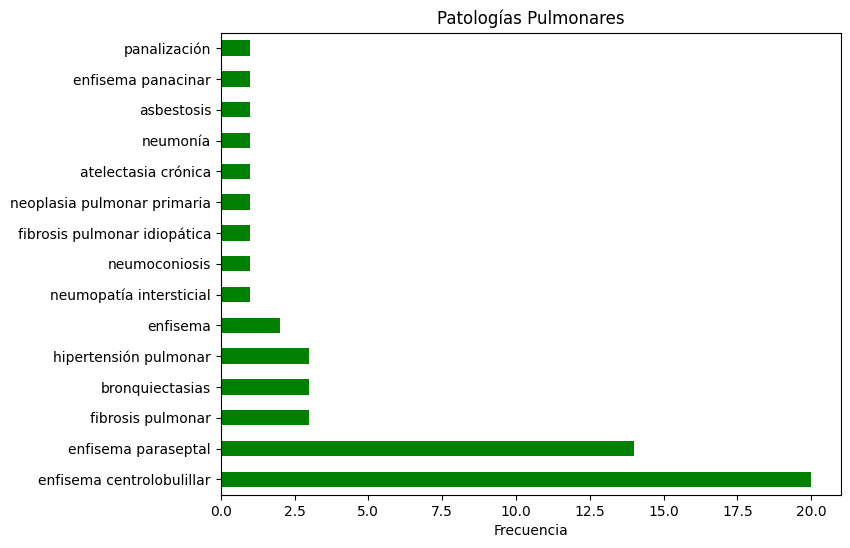
\includegraphics[width=1\textwidth]{img/barras_patologia_pulmonar.png}
    \caption{Frecuencia de categorías en Patología pulmonar.}
    \label{fig:distribucion_patologia_pulmonar}
\end{figure}


\begin{figure}[!htbp]
    \centering
    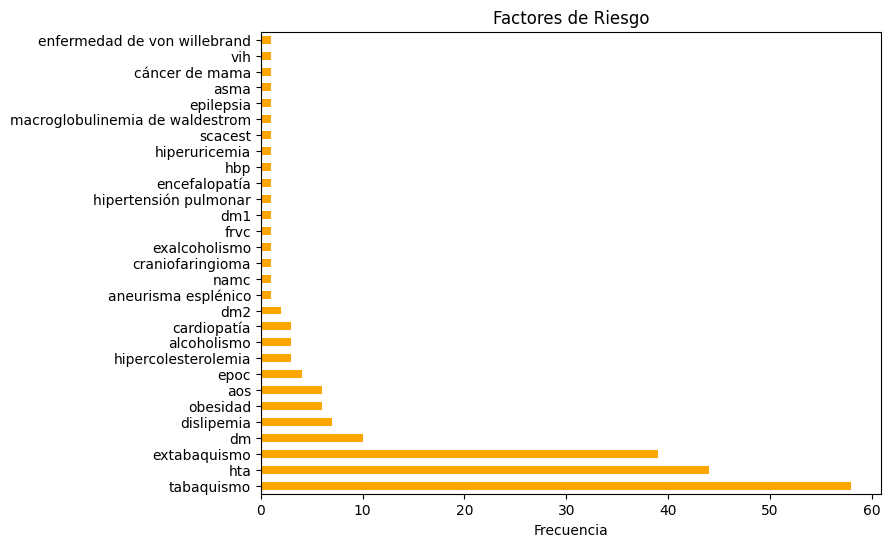
\includegraphics[width=1\textwidth]{img/barras_factor_riesgo.png}
    \caption{Frecuencia de categorías en Factor de riesgo.}
    \label{fig:distribucion_factor_riesgo}
\end{figure}


El análisis de estas variables evidencia una considerable diversidad y riqueza semántica, lo que justifica la necesidad de aplicar un preprocesamiento multietiqueta para transformarlas en variables utilizables en un modelo de aprendizaje automático.

En conclusión, el análisis de los datos clínicos confirma la ausencia de valores nulos, un ligero desbalanceo de clases y una población predominantemente mayor.




% ----------------------------------------------------------------------

\section{Preprocesamiento de los datos} \label{sec:preprocesamiento}

Tras el análisis exploratorio, se realizó el preprocesamiento en Python adaptado a las características del dataset, con el objetivo de estandarizar el formato de entrada y reducir la variabilidad innecesaria que pudiera afectar al entrenamiento de modelos. Este preprocesamiento abarca tanto los datos clínicos tabulares como los volúmenes de imagen médica en formato DICOM, asegurando una preparación coherente y homogénea de todas las fuentes de datos.

\subsection{Preprocesamiento de datos de volúmenes DICOM}

\subsubsection{Introducción a MONAI para el modelado de imágenes médicas}

Para los volúmenes DICOM se utilizó principalmente MONAI, una biblioteca especializada en el procesamiento y modelado de imágenes médicas. Se implementó un preprocesamiento modular basado en MONAI, complementado con transformaciones personalizadas adaptadas al dominio clínico. Los pipelines se construyeron de forma modular y configurable, definiendo versiones para entrenamiento y validación. 

\subsubsection{Igualación de tamaños de imágenes}

Para abordar la alta variabilidad en la forma de los volúmenes (con diferente número de cortes y resoluciones como 512x512 o 768x768), se empleó una interpolación trilineal para normalizar todos los volúmenes a un tamaño objetivo uniforme. Esto asegura entradas de tamaño constante, crucial para el entrenamiento de redes convolucionales 3D. La interpolación trilineal preserva la continuidad espacial y anatómica, manteniendo la coherencia del volumen.

Se exploraron diferentes tamaños para estos volúmenes, evaluando su impacto en el entrenamiento. Inicialmente, se utilizaron resoluciones grandes como (256,512,512) o (128,256,256), con el objetivo de preservar el mayor detalle posible. Sin embargo, en los análisis con técnicas de explicabilidad se observó que el modelo a menudo se fijaba en regiones irrelevantes, posiblemente debido al exceso de información redundante. Por ello, se ensayaron también resoluciones más reducidas, como (128,128,128), (64,64,64) e incluso (28,28,28). Estos tamaños más compactos ayudaban a forzar al modelo a centrarse en patrones globales más relevantes y a mitigar el sobreajuste a detalles poco útiles. No obstante, las resoluciones más pequeñas como (28,28,28) se descartaron por perder demasiado detalle anatómico. Fueron inicialmente utilizadas por similitud a datasets para preentrenamiento, ya que utilizaban imágenes médicas de ese tamaño. 

\subsubsection{Data augmentation}

Se han probado diferentes tipos de preprocesamiento, uno de ellos incluye también transformaciones de data augmentation como \texttt{RandAffine}, que aplica rotaciones, escalados y traslaciones aleatorias, simulando variabilidad anatómica y de posicionamiento del paciente. Estas transformaciones son leves para no distorsionar demasiado las imágenes, mejorando así la capacidad de generalización del modelo al exponerlo a ligeras variaciones geométricas de los datos de entrenamiento.

\subsubsection{Ventanas de Hounsfield}

En TC, el valor de cada voxel en la imagen reconstruida refleja el coeficiente de atenuación lineal del haz de rayos X al atravesar el tejido correspondiente \parencite{calzado2010tomografia}. Para estandarizar su interpretación, estos coeficientes se transforman en la escala de \textit{unidades Hounsfield (HU)}, que usa el agua a temperatura ambiente como referencia de 0 HU y el aire como -1000 HU. Esta transformación se define mediante la fórmula:

\[
HU_{mat} = \frac{\mu_{mat} - \mu_{agua}}{\mu_{agua}} \times 1000
\]

donde $\mu_{mat}$ es el coeficiente de atenuación lineal del material o tejido y $\mu_{agua}$ el del agua. Cada incremento de 1 HU corresponde a un cambio del 0,1\% en la atenuación relativa al agua.  

La escala Hounsfield abarca un rango amplio de valores: el aire se define como -1000 HU (pues apenas atenúa), el agua como 0 HU, y el tejido adiposo suele encontrarse entre -100 y -80 HU. El parénquima pulmonar se sitúa aproximadamente entre -950 y -600 HU, mientras que la mayoría de tejidos blandos se representan con valores de 20 a 70 HU. Por su parte, el hueso compacto puede superar los +1000 HU, reflejando su elevada densidad.

En la adquisición de imágenes, los escáneres suelen almacenar estos valores con una profundidad mínima de 12 bits, cubriendo un rango aproximado de -1024 a +3071 HU, suficiente para la mayoría de tejidos clínicos. Sin embargo, algunas aplicaciones utilizan 14 bits para ampliar esta escala hasta más de +15.000 HU, permitiendo representar materiales de alta densidad, como implantes metálicos, stents o prótesis ortopédicas, sin saturación en la imagen.

Para visualizar estas imágenes en monitores médicos, que suelen limitarse a 8 o 12 bits (256 o 4096 niveles de gris), se utiliza el concepto de \textit{ventana de visualización}. Esta técnica permite ajustar el rango de HU mostrado para optimizar la visualización de diferentes tipos de tejidos. Está caracterizada por dos parámetros fundamentales:

\begin{itemize}
    \item \textbf{Window Level (WL)}: nivel central de la ventana, que define qué valor de HU aparecerá como gris medio.
    \item \textbf{Window Width (WW)}: ancho de la ventana, que determina el rango total de HU representado desde negro hasta blanco.
\end{itemize}

Al ajustar WL y WW, los radiólogos pueden resaltar estructuras específicas. Por ejemplo, en el análisis del parénquima pulmonar se suelen usar ventanas con WL $\approx$ -600 HU y WW $\approx$ 1500 HU para resaltar lesiones como nódulos, consolidaciones o enfisema (veáse la Figura \ref{fig:hu-ejemplo}). Para tejidos blandos del mediastino o abdomen se usan combinaciones distintas de WL y WW para optimizar el contraste en esas estructuras.

Sin embargo, los valores de HU pueden verse afectados por diversos factores técnicos: la tensión del tubo de rayos X (kVp) influye en la atenuación relativa, sobre todo en materiales de alto número atómico como el hueso (calcio) o el contraste yodado; además, el filtro de reconstrucción, el campo de visión (FOV), la posición del objeto escaneado o incluso artefactos pueden introducir variaciones en los valores registrados. A esto se suman posibles desviaciones sistemáticas entre equipos diferentes o la deriva temporal de un mismo escáner. Por ello, en estudios multicéntricos o longitudinales se requiere especial cuidado en la calibración y armonización de los valores HU para garantizar la comparabilidad cuantitativa.

Para este proyecto, se han diseñado transformaciones específicas en el pipeline de MONAI que aplican de forma sistemática y reproducible las ventanas clínicas relevantes. Estas transformaciones recortan los valores de HU a rangos clínicamente significativos y los normalizan al intervalo [0,1], facilitando el aprendizaje del modelo al centrarse en la información más útil. En concreto, se implementaron dos enfoques principales:

\begin{itemize}
    \item \textbf{Windowingd}: aplica una única ventana (por ejemplo, la ventana pulmonar), generando un canal de entrada optimizado para resaltar el parénquima y sus lesiones.
    \item \textbf{MultiWindowingd}: aplica varias ventanas (pulmón, mediastino, consolidación) y apila los resultados como canales independientes, creando una representación multicanal que enriquece la información anatómica y patológica disponible para el modelo.
\end{itemize}

\begin{figure}[!htbp]
    \centering
    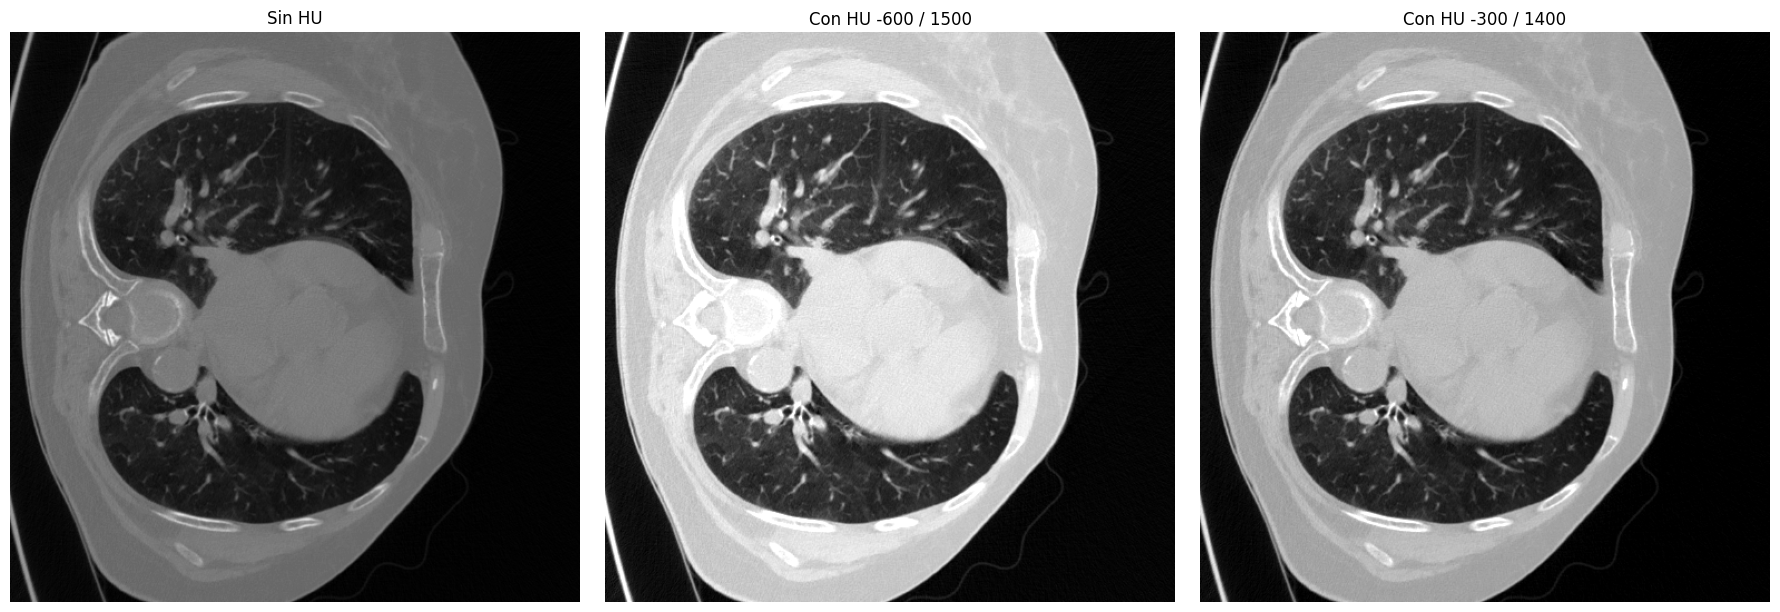
\includegraphics[width=1\textwidth]{img/hu_ejemplos.png}
    \caption{Comparación de la misma imagen axial de TC preprocesada con diferentes configuraciones de ventana HU: sin ventana, con ventana centrada en -600 HU (ancho 1500) y con ventana centrada en -300 HU (ancho 1400). Se observa la mejora de contraste en el parénquima pulmonar tras aplicar el recorte de intensidades. Elaboración propia.}
    \label{fig:hu-ejemplo}
\end{figure}

Estas estrategias imitan el proceso diagnóstico clínico, donde el radiólogo ajusta las ventanas para identificar con mayor claridad las estructuras relevantes, mejorando así la interpretabilidad y el rendimiento del modelo en tareas de clasificación o segmentación.

\subsubsection{Segmentación}

Durante las primeras fases de experimentación se utilizaron los volúmenes 3D originales de TC sin ningún tipo de segmentación previa. Sin embargo, al aplicar técnicas de explicabilidad y analizar los mapas de activación de los modelos, se observó que en numerosas ocasiones el modelo se fijaba en regiones externas al pulmón. Esto introducía un sesgo importante, ya que la red podía aprender patrones irrelevantes y no relacionados con las complicaciones pulmonares que se pretendían predecir.

Para mitigar este problema y forzar al modelo a centrarse únicamente en la región anatómica de interés, se incorporó un paso de \textit{segmentación pulmonar}. La segmentación permite aislar el volumen pulmonar, eliminando estructuras irrelevantes y reduciendo el ruido de fondo. De esta forma, se mejora la capacidad del modelo para aprender patrones verdaderamente discriminativos y clínicamente relevantes.

La generación de máscaras de pulmón se realizó de forma completamente automatizada utilizando la herramienta \texttt{TotalSegmentator} \parencite{wasserthal2023totalsegmentator}, una solución basada en aprendizaje profundo que ofrece modelos preentrenados para segmentación médica. En este caso, se empleó la tarea específica de segmentación pulmonar, que produce máscaras binarias indicando únicamente la localización de los pulmones en cada volumen. Se pueden observar dos ejemplos de esta segmentación (uno en 2D y otro en 3D) en las Figura \ref{fig:ejemplo-segmentacion} y \ref{fig:ejemplo-segmentacion3D}. Los datos DICOM originales se convirtieron previamente al formato NIfTI (.nii) para compatibilidad con el modelo, y las máscaras generadas se almacenaron con nomenclatura estandarizada para su posterior uso.

Una vez generadas las máscaras pulmonares, se integraron en el flujo de preprocesamiento mediante la transformación \texttt{CombineMaskAndImage}. Esta operación permite combinar la imagen original y su máscara segmentada de dos formas principales: 
\begin{itemize}
    \item \textbf{stack}: apilando la máscara como un canal adicional para que el modelo disponga explícitamente de la información sobre la localización pulmonar.
    \item \textbf{mask\_zero\_out}: enmascarando las regiones externas al pulmón con valores HU muy bajos, forzando al modelo a ignorar información irrelevante.
\end{itemize}
Esta flexibilidad permite experimentar con diferentes enfoques, desde obligar a la red a centrarse solo en el pulmón.

\subsection{Preprocesamiento de datos clínicos tabulares}

Para los datos clínicos tabulares se utilizó la biblioteca scikit-learn de Python. El proceso comenzó con la eliminación de columnas que contenían información únicamente disponible \textit{a posteriori}, como el \textit{Tipo de cáncer}, evitando así la introducción de fugas de información en el entrenamiento. Posteriormente, se abordó el tratamiento de variables multietiqueta, como \textit{Factor de riesgo} y \textit{Patología pulmonar}. Estas columnas incluían múltiples etiquetas separadas por comas, lo que requería una limpieza para unificar nomenclaturas y corregir inconsistencias. Además, se reemplazaron valores nulos o el marcador especial \texttt{X} por etiquetas explícitas como \textit{Sin complicación} o \textit{Sin factor de riesgo}. Para transformar estos datos en un formato apto para modelos de aprendizaje automático, se aplicó un esquema de binarización multietiqueta mediante \texttt{MultiLabelBinarizer}, generando variables one-hot que representan la presencia o ausencia de cada etiqueta.

La variable \textit{Edad} fue normalizada en el rango [0,1] utilizando \texttt{MinMaxScaler}, para evitar problemas de escala y facilitar el aprendizaje del modelo. Además, la variable objetivo \textit{Complicación}, originalmente categórica con valores \textit{Sí o No}, se transformó en binaria asignando \textit{1 o 0} respectivamente. Como resultado final, se obtuvo un conjunto de datos tabular limpio y consistente, con variables numéricas y binarias, libre de valores nulos y con un formato adecuado para entrenamiento, que se almacenó en formato CSV para uso posterior.

\begin{figure}[!htbp]
    \centering
    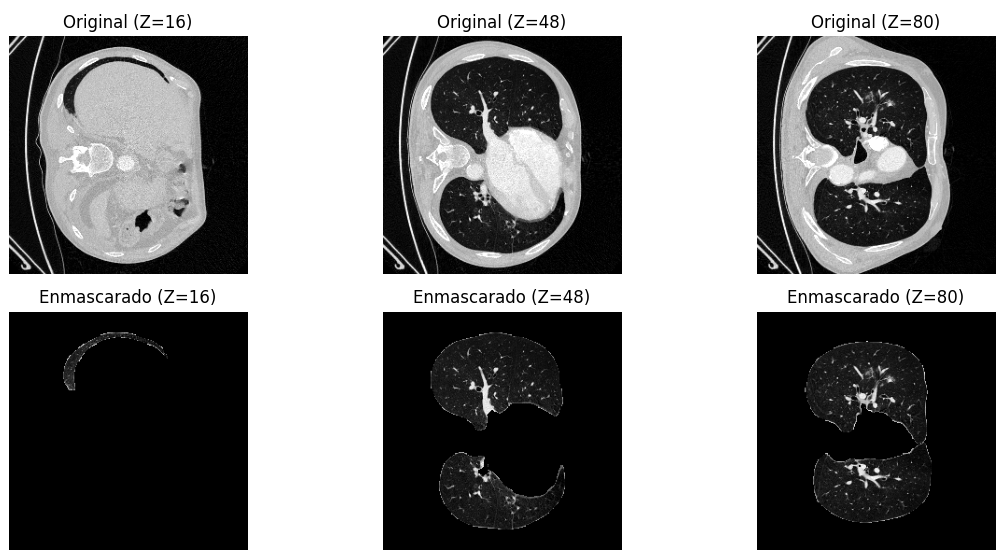
\includegraphics[width=1\textwidth]{img/ejemplo_segmentacion.png}
    \caption{Ejemplo de un volumen antes y después de la segmentación. Elaboración propia.}
    \label{fig:ejemplo-segmentacion}
\end{figure}

\begin{figure}[!htbp]
    \centering
    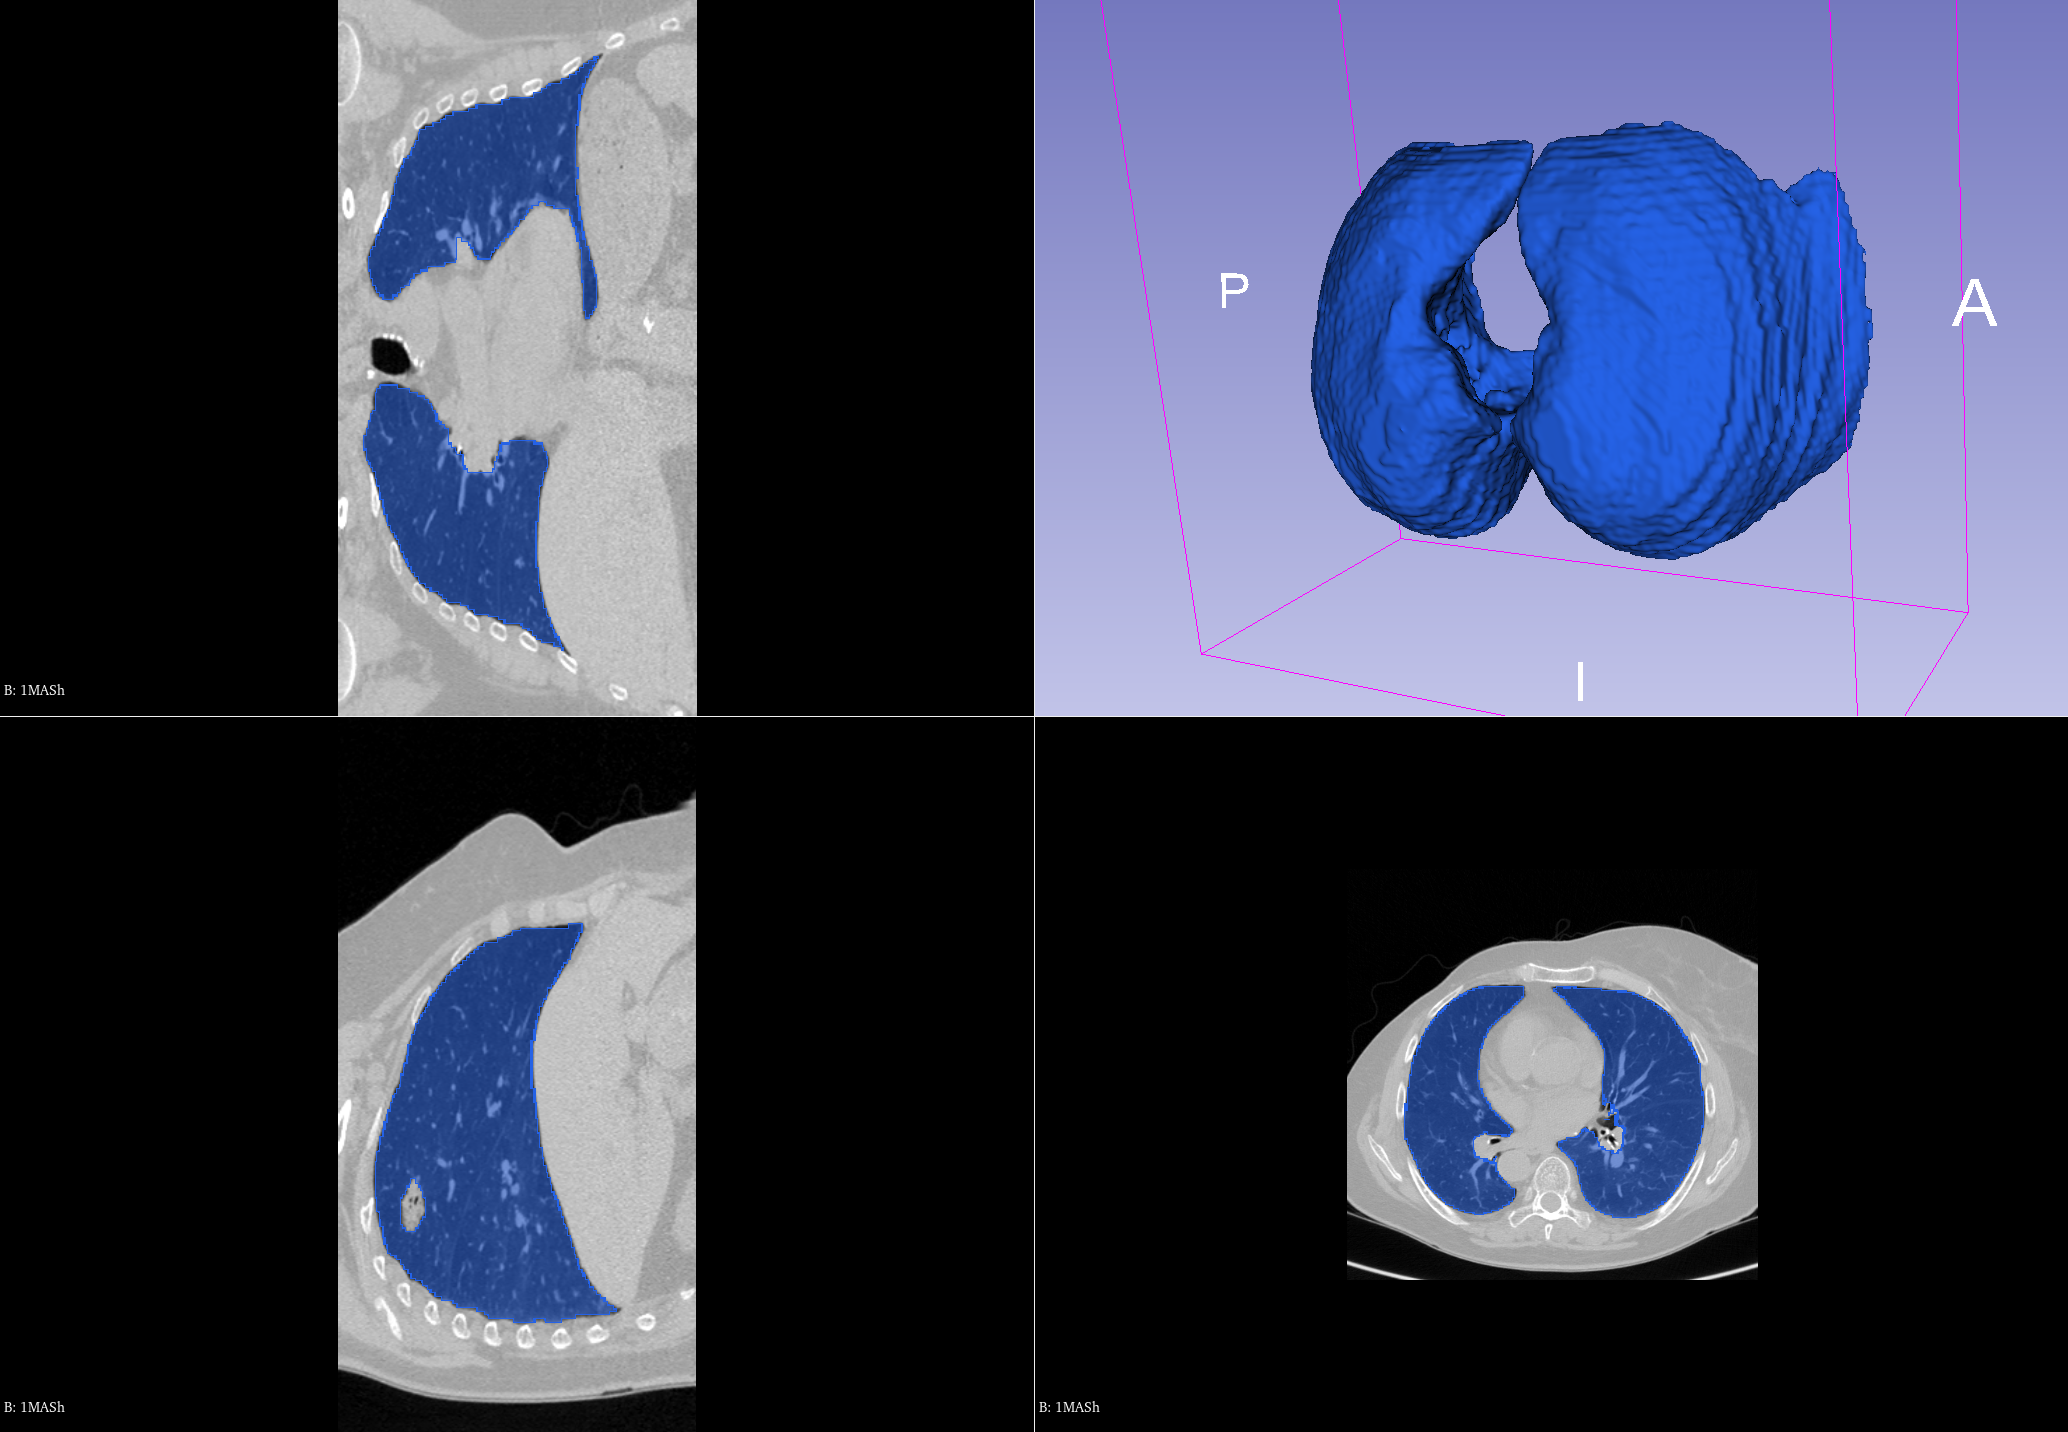
\includegraphics[width=1\textwidth]{img/segmentacion3D.png}
    \caption{Ejemplo de segmentación en 3D y en los 3 planos anatómicos en 2D. Elaboración propia realizada con 3D Slicer.}
    \label{fig:ejemplo-segmentacion3D}
\end{figure}


\endinput
%--------------------------------------------------------------------
% FIN DEL CAPÍTULO. 
%--------------------------------------------------------------------

% !TeX root = ../tfg.tex
% !TeX encoding = utf8

\chapter{Técnicas de Deep Learning} \label{chap:dl-info}

En este capítulo se describen las principales estrategias probadas de deep learning para abordar el problema de la predicción de complicaciones en biopsias pulmonares a partir de datos de tomografía computarizada. Se presentan tanto los enfoques iniciales basados en cortes bidimensionales (2D) como la evolución hacia modelos tridimensionales (3D) que aprovechan de forma completa la información volumétrica de las imágenes.  

\section{Enfoque basado en cortes 2D}

En las fases iniciales del proyecto se planteó abordar el problema utilizando modelos convolucionales 2D entrenados sobre cortes axiales extraídos de los volúmenes de TC. Se empezó por esta técnica ya que computacionalmente conllevaba menos requisitos. Esto se debe a que los modelos 2D son más ligeros, rápidos de entrenar y pueden aprovechar pesos preentrenados en tareas de visión convencional.

El procedimiento consistía en dividir cada volumen 3D en múltiples cortes axiales, que se preprocesaban de forma individual para usarse como muestras independientes durante el entrenamiento. El objetivo era que el modelo aprendiera a clasificar cada corte según la presencia o ausencia de complicaciones. Sin embargo, esto planteaba varios desafíos importantes: por un lado, la predicción debía agregarse finalmente a nivel de paciente, no de corte aislado; por otro, al tratarse de volúmenes reales, muchas de las slices correspondían a regiones extremas sin tejido pulmonar visible, lo que introducía información confusa y dificultaba el aprendizaje efectivo del modelo.

Otras de las limitaciones de este enfoque es que al trabajar con slices individuales, se pierde la información espacial tridimensional presente en el volumen completo. La relación entre cortes consecutivos, que puede contener patrones anatómicos relevantes para predecir complicaciones, queda ignorada. Además, la variabilidad en el número de cortes entre pacientes complica la agregación de predicciones y la estandarización.

Debido a estos factores, y especialmente a los malos resultados obtenidos en las primeras pruebas, se decidió descartar rápidamente esta aproximación en favor de un enfoque 3D para aprovechar la naturaleza de los datos.


\subsection{Descripción de las arquitecturas empleadas 2D}

\subsubsection{EfficientNetV2}
EfficientNetV2  \parencite{tan2021efficientnetv2} es una familia de redes neuronales convolucionales diseñadas para ser especialmente eficientes en términos de velocidad de entrenamiento y uso de recursos computacionales. Su principal objetivo es lograr un buen equilibrio entre precisión, tamaño del modelo y tiempo de entrenamiento, aspectos especialmente importantes cuando se dispone de recursos limitados o se buscan aplicaciones prácticas en entornos clínicos.

A diferencia de modelos anteriores más pesados, EfficientNetV2 introduce mejoras en la forma en que se organiza y escala la arquitectura. En lugar de simplemente hacer la red más profunda o ancha de manera uniforme, aplica un \textit{escalado compuesto} más inteligente, que distribuye la complejidad donde más se necesita. Esto significa que se añaden capas de forma más selectiva en determinadas etapas de la red, optimizando el uso de parámetros y reduciendo el tiempo de entrenamiento sin sacrificar precisión.

Además, este modelo introduce bloques de convolución más simples y rápidos, llamados \textit{Fused-MBConv}, que combinan de forma eficiente operaciones convolucionales para reducir la sobrecarga de memoria y acelerar el entrenamiento. La estructura de estos bloques está representada en la Figura \ref{fig:efficientnetv2}. Esta simplificación permite entrenar modelos de buena capacidad en menos tiempo.

En este proyecto se utilizó la variante \texttt{EfficientNetV2-S}, una configuración compacta y rápida, pensada para ofrecer un rendimiento competitivo sin alzar mucho el coste computacional. Es por eso por lo que hemos elegido esta red frente a otras, ya que resulta adecuada para trabajar con imágenes 2D de cortes axiales, donde la eficiencia es clave para poder procesar grandes volúmenes de datos en tiempos razonables.

\begin{figure}[!htbp]
    \centering
    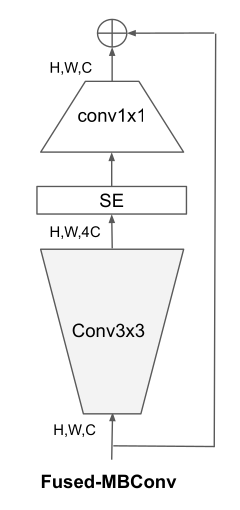
\includegraphics[width=0.25\textwidth]{img/efficientnetv2.png}
    \caption{Estructura de Fused-MBConv \parencite{tan2021efficientnetv2}.}
    \label{fig:efficientnetv2}
\end{figure}


\section{Enfoque basado en volúmenes 3D}

Dada la naturaleza volumétrica de los datos de TC, un enfoque más adecuado consiste en procesar directamente el volumen tridimensional completo. Para ello, utilizamos redes neuronales convolucionales 3D que extienden las operaciones de convolución y pooling clásicas a tres dimensiones, trabajando sobre la altura, anchura y profundidad (número de slices).

En general, muchas arquitecturas 2D pueden adaptarse a 3D de forma relativamente directa, sustituyendo las capas de convolución 2D por convoluciones 3D (con kernels típicos de $3 \times 3 \times 3$) y aplicando pooling 3D. Esto permite a la red capturar patrones espaciales en las tres dimensiones. Las dos arquitecturas empleadas en este trabajo, \textit{ResNet} y \textit{DenseNet} han sido adaptadas a este formato, manteniendo la esencia de sus diseños originales pero generalizando sus operaciones al espacio tridimensional.

Un aspecto importante para trabajar con volúmenes 3D es la necesidad de normalizar el tamaño de entrada. Los volúmenes originales, como vimos en la sección \ref{eda} presentan variabilidad en el número de slices y resolución axial (512x512 o 768x768). En la propia sección, en el preprocesamiento, se realizó interpolación trilineal para estandarizar todos los volúmenes a un tamaño (se realizaron múltiples interpolaciones para poder probar diferentes tamaños). Esto es esencial para permitir el procesamiento en batch y la compatibilidad con arquitecturas convolucionales profundas.

\subsection{Procedimiento general de entrenamiento}

El procedimiento seguido es muy común en aprendizaje profundo pero con adaptaciones necesarias para trabajar con imágenes médicas volumétricas y un dataset relativamente pequeño.

En primer lugar, se define la arquitectura del modelo. En este trabajo se utilizó principalmente DenseNet121 adaptado a 3D, una arquitectura que incluye bloques densos con conexiones entre todas las capas, lo que mejora la propagación de gradientes y favorece la reutilización de características. 

Durante el entrenamiento, se emplea un enfoque supervisado clásico, utilizando la \textit{CrossEntropyLoss} como función de pérdida para la tarea de clasificación binaria (complicación sí/no). El optimizador más usado fue \textit{Adam}, conocido por ser efectivo con datos heterogéneos y tamaños de batch reducidos. En algunas configuraciones, se experimentó con \textit{weight decay} para ayudar a evitar el sobreajuste.

Para cada fold, se entrena el modelo durante varias épocas monitorizando métricas clave en el conjunto de validación, como accuracy, F1-score o G-Mean, para identificar el modelo con mejor desempeño. Además, se aplican técnicas como \textit{early stopping} y ajustes de regularización como dropout para mitigar el sobreajuste dada la limitada cantidad de datos.

Adicionalmente, se aplicaron técnicas de explicabilidad como Grad-CAM o Shap para analizar las regiones de los volúmenes en las que el modelo basaba sus decisiones, asegurando así que el aprendizaje se centraba en el tejido pulmonar relevante y no en artefactos o regiones externas. 

En resumen, el entrenamiento de los modelos se diseñó de forma modular con optimización, regularización y validación, adaptadas al nuestro problema específico con datos 3D limitados.



\subsection{Descripción de las arquitecturas empleadas 3D}
Durante toda la fase de implementación se han probado varios modelos. Los dos principales son ResNet3D y DenseNet121 3D. 

\subsubsection{Resnet}
Las 3D ResNets (Residual Networks) son una extensión natural de las ResNets 2D al dominio volumétrico \parencite{hara2017learning}. Conservan la idea clave de las \textit{conexiones de salto} (skip connections), que ayudan a mitigar el problema del gradiente desvanecido al permitir un flujo de información más directo entre capas distantes.  

En su adaptación 3D, tanto las convoluciones como las operaciones de pooling se aplican en las tres dimensiones espaciales. Por ejemplo, se utilizan kernels convolucionales de $3 \times 3 \times 3$, y el downsampling se realiza con stride 2 en todas las dimensiones. Esto permite a la red capturar contextos espaciales tridimensionales completos, cruciales en tareas como la segmentación o la predicción de riesgos en TC. Su arquitectura se puede observar en la Tabla \ref{tab:resnet_arch}.

Las 3D ResNets han demostrado ser más precisas que arquitecturas más simples, especialmente cuando se dispone de suficiente capacidad de cómputo y datos bien preprocesados.


\begin{table}[!htbp]
\centering
\caption{Arquitectura ResNet 3D. Los bloques residuales se muestran entre paréntesis. Cada capa convolucional va seguida de normalización por lotes y ReLU. El muestreo descendente se realiza mediante conv3\_1, conv4\_1, conv5\_1 con un paso de 2. La dimensión de la última capa totalmente conectada se establece para el conjunto de datos Kinetics (400 categorías) \parencite{hara2017learning}.}
\label{tab:resnet_arch}
\begin{tabular}{ccc}
\hline
Nombre de la capa & Arquitectura (18-layer) & Arquitectura (34-layer) \\
\hline
conv1 & $7 \times 7 \times 7$, 64, stride 1 (T), 2 (XY) & \\
\hline
conv2\_x & 3 $\times$ 3 $\times$ 3 max pool, stride 2 &  \\
         & $\left[\begin{array}{c}
         3 \times 3 \times 3, 64 \\
         3 \times 3 \times 3, 64
         \end{array}\right] \times 2$ &
         $\left[\begin{array}{c}
         3 \times 3 \times 3, 64 \\
         3 \times 3 \times 3, 64
         \end{array}\right] \times 3$ \\
\hline
conv3\_x & $\left[\begin{array}{c}
         3 \times 3 \times 3, 128 \\
         3 \times 3 \times 3, 128
         \end{array}\right] \times 2$ &
         $\left[\begin{array}{c}
         3 \times 3 \times 3, 128 \\
         3 \times 3 \times 3, 128
         \end{array}\right] \times 4$ \\
\hline
conv4\_x & $\left[\begin{array}{c}
         3 \times 3 \times 3, 256 \\
         3 \times 3 \times 3, 256
         \end{array}\right] \times 2$ &
         $\left[\begin{array}{c}
         3 \times 3 \times 3, 256 \\
         3 \times 3 \times 3, 256
         \end{array}\right] \times 6$ \\
\hline
conv5\_x & $\left[\begin{array}{c}
         3 \times 3 \times 3, 512 \\
         3 \times 3 \times 3, 512
         \end{array}\right] \times 2$ &
         $\left[\begin{array}{c}
         3 \times 3 \times 3, 512 \\
         3 \times 3 \times 3, 512
         \end{array}\right] \times 3$ \\
\hline
\multicolumn{3}{c}{average pool, 400-d fc, softmax} \\
\hline
\end{tabular}
\end{table}




\subsubsection{Arquitectura DenseNet-121}

DenseNet (Densely Connected Convolutional Network) propone un esquema de conectividad densa en el que cada capa recibe como entrada todos los mapas de características de las capas anteriores, favoreciendo la reutilización de características y mejorando el flujo de gradientes \parencite{huang2017densely}. Esta idea también puede extenderse de forma natural al dominio tridimensional. Véase Figuras \ref{fig:densenet2} y \ref{fig:densenet1}.

En la versión 3D de DenseNet-121, todas las convoluciones 2D se sustituyen por convoluciones 3D, manteniendo la estructura en bloques densos y capas de transición con pooling 3D. Este diseño permite capturar patrones volumétricos complejos y facilita el aprendizaje de representaciones más expresivas con menos parámetros, aprovechando la reutilización de características intermedias.  

Una característica importante es la inclusión de capas bottleneck (convoluciones 1x1x1) que reducen el número de canales de entrada, esto simplifica el modelo sin alterar la resolución espacial, antes de aplicar convoluciones más costosas de 3x3x3. Además, se emplean capas de transición con average pooling para reducir progresivamente la resolución espacial del volumen.

\begin{figure}[!htbp]
    \centering
    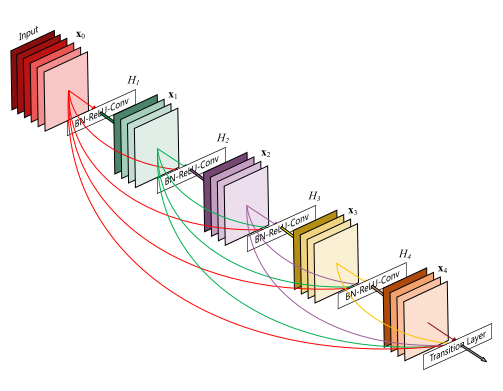
\includegraphics[width=0.7\textwidth]{img/densenet121_2.png}
    \caption{Un bloque denso de 5 capas con una tasa de crecimiento de $k=4$. Cada capa toma como entrada todos los mapas de características anteriores \parencite{huang2017densely}.}
    \label{fig:densenet2}
\end{figure}


\begin{figure}[!htbp]
    \centering
    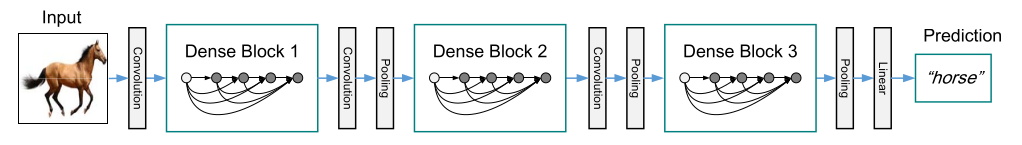
\includegraphics[width=1\textwidth]{img/densenet121_1.png}
    \caption{Una DenseNet profunda con tres bloques densos. Las capas entre dos bloques adyacentes se denominan capas de transición y cambian el tamaño de los mapas de características de
mediante convolución y agrupación \parencite{huang2017densely}.}
    \label{fig:densenet1}
\end{figure}

En conjunto, este enfoque 3D resultó más adecuado para el problema planteado, ya que preserva la información tridimensional completa del pulmón, permitiendo al modelo aprender relaciones espaciales relevantes para la predicción del riesgo de complicaciones tras la biopsia.

\section{Técnicas avanzadas}

\subsection{Pre-entrenamiento en otras tareas similares y fine-tuning}
Uno de los principales desafíos de este proyecto, y en general de muchos trabajos en el ámbito médico, es el tamaño limitado de la base de datos disponible, compuesta en este caso por tan solo 125 pacientes. Este volumen de datos puede resultar insuficiente para entrenar desde cero modelos de deep learning como los descritos anteriormente, ya que puede conducir al sobreajuste o poca generalización.

Para mitigar este problema, se emplea habitualmente una estrategia conocida como \textit{preentrenamiento (pretraining)}, que consiste en entrenar previamente el modelo sobre datos relacionados o tareas similares. De este modo, el modelo parte de un conocimiento inicial que puede facilitar el aprendizaje en la tarea específica y mejorar los resultados finales. Posteriormente, se aplica un \textit{ajuste fino (fine-tuning)}, técnica ampliamente utilizada en aprendizaje profundo para adaptar el conocimiento aprendido en la tarea fuente al dominio objetivo.

El fundamento del preentrenamiento es inicializar el modelo con pesos entrenados previamente en un problema relacionado y con mayor disponibilidad de datos, de forma que la red haya aprendido representaciones generales útiles para la nueva tarea. En este trabajo, se utilizó un conjunto de datos abierto y público, \textit{MedMNIST3D}, que incluye volúmenes de TC asociados a distintas tareas de clasificación anatómica. Aunque las etiquetas de la tarea fuente (órganos o estructuras) no son equivalentes al problema de predicción de complicaciones en biopsias pulmonares, la hipótesis es que el modelo puede aprender características morfológicas y texturales generales del pulmón y otras estructuras corporales que resulten transferibles. Incluso podría captar patrones sutiles que contribuyan a mejorar el rendimiento en nuestro conjunto de datos.

Durante el preentrenamiento se usaron arquitecturas 3D convolucionales (ResNet3D y DenseNet121 3D) entrenadas para tareas de clasificación multiclase en MedMNIST3D. Para obtener el mejor modelo preentrenado, se combinaron diferentes funciones de pérdida, incluyendo \textit{Cross-Entropy}, \textit{Triplet Loss} y \textit{Contrastive Loss} (véase \ref{subsec:pre-contrastivo}), con el objetvo de mejorar la separación entre clases y facilitar su utilidad para transferencia. Todo este entrenamiento se realizó de forma supervisada y con estrategias de data augmentation específicad del dominio 3D.

Una vez finalizado el preentrenamiento, se realizó el ajuste fino (\textit{fine-tuning}) sobre la tarea objetivo: predicción de complicaciones tras biopsia pulmonar. Para ello, se cargaron los pesos preentrenados y se entrenó el modelo en nuestro conjunto de datos. Se evaluaron dos estrategias principales de fine-tuning:

\begin{itemize}
    \item \textbf{Fine-tuning con el backbone congelado:} únicamente se reentrenó la capa de clasificación final. Esta opción tiene la ventaja de evitar el sobreajuste en datasets muy pequeños, limitando el número de parámetros a actualizar.
    \item \textbf{Fine-tuning completo (todo descongelado):} todos los pesos del modelo fueron reentrenados con un learning rate más bajo que en experimentos con modelos sin preentrenar. Esta estrategia permite adaptar mejor las características intermedias del modelo al dominio específico de nuestros volúmenes.
\end{itemize}

Ambas variantes se evaluaron mediante validación cruzada estratificada para medir su capacidad de generalización, comparando métricas como Accuracy, F1-score y G-Mean. 

Si bien en teoría esta técnica debería mejorar el rendimiento, en nuestro caso los modelos preentrenados no lograron superar el rendimiento de los entrenados desde cero (véase el Capítulo \ref{analisis-resultados}). Este resultado puede deberse a que nuestra tarea es muy específica y difiere considerablemente de la tarea fuente. También puede ser que el preentrenamiento haya inducido al modelo a aprender características generales que no resultan suficientemente informativas para nuestro problema concreto.

\subsection{Pre-entrenamiento contrastivo y Deep Metric Learning} \label{subsec:pre-contrastivo}

En la gran mayoría de las implementaciones de estre trabajo hemos utilizado la función de pérdida de entropía cruzada. Incluso en general también son ampliamente utilizadas en muchas aplicaciones de aprendizaje profundo supervisado. Sin embargo, tienden a ser menos adecuados cuando existe una gran varianza intraclase y una baja varianza interclase en la distribución de los datos de entrada. Aquí es cuando surge el concepto de  \textit{Aprendizaje profundo métrico (Deep Metric Learning)} \parencite{mohan2023deep}. El aprendizaje profundo métrico tiene como objetivo que el modelo aprenda a medir la similitud entre muestras al proyectarlas en un espacio de representación donde las relaciones entre clases estén bien estructuradas. En este espacio, las muestras de la misma clase se ubican próximas entre sí, mientras que las de clases diferentes se mantienen separadas. Para lograrlo, se utilizan estrategias de muestreo adecuadas y funciones de pérdida específicas que optimizan la construcción de este espacio, incluso en escenarios donde las clases presentan diferencias sutiles o alta variabilidad interna.

Las dos funciones de pérdida que hemos utilizado en el preentrenamiento han sido \textit{Contrastive Loss} y \textit{Triplet Loss} explicadas matemáticamente en la Sección \ref{sec:contrastive-loss}.

% \subsubsection{Contrastive Loss}

% El objetivo principal de una formulación estándar de \textit{metric learning} es aprender un espacio de representación donde muestras de la misma clase estén cercanas entre sí, mientras que las de clases distintas se mantengan alejadas. Una manera de imponer esta restricción durante el entrenamiento de una red neuronal profunda es mediante la \textit{Contrastive Loss}.  

% Consideremos dos representaciones de características, $f_i$ y $f_j$, asociadas a las muestras $i$ y $j$. Si ambas pertenecen a la misma clase, el objetivo es minimizar la distancia entre sus representaciones. En cambio, si pertenecen a clases distintas, se busca maximizar la distancia al menos hasta un margen $\alpha$. Matemáticamente, la función de pérdida contrastiva se define como:

% \[
% L_{con} = 
% \begin{cases}
% \|f_i - f_j\|^2, & \text{si } y_i = y_j \\
% \left[\alpha - \|f_i - f_j\|^2\right]_+, & \text{si } y_i \neq y_j
% \end{cases}
% \]

% donde $y_i$ y $y_j$ son las clases asociadas a las muestras $i$ y $j$, y $\alpha$ es el margen que determina la distancia mínima deseada entre clases distintas. El operador $[\,\cdot\,]_+$ denota la función \textit{max}($0$, $\cdot$), que asegura no penalizar distancias ya mayores al margen.

% Esta formulación fuerza al modelo a aprender un espacio de características donde las muestras de la misma clase queden agrupadas, mientras que las de diferentes clases se separen al menos una distancia $\alpha$, favoreciendo así la discriminación en el espacio de representación aprendido.

% \vspace{1em}

% \subsubsection{Triplet Loss}

% La \textit{Triplet Loss} es una mejora sobre la formulación de la Contrastive Loss, ampliamente utilizada como objetivo en aprendizaje métrico para crear espacios de incrustación más separables. Esta pérdida considera tres representaciones de características: $f_a$, $f_p$ y $f_n$, correspondientes a una imagen ancla (Anchor), una positiva (Positive) y una negativa (Negative) respectivamente.  

% El par ancla-positiva $(a,p)$ corresponde a dos muestras de la misma clase, mientras que la muestra negativa $n$ pertenece a una clase diferente. El objetivo de la Triplet Loss es minimizar la distancia entre el Anchor y el Positive, al mismo tiempo que se maximiza la distancia entre el Anchor y el Negative, garantizando al menos un margen $\alpha$ de separación.  

% Cuando se utiliza la distancia euclidiana, la formulación de la Triplet Loss es:

% \[
% \mathcal{L} = \sum_{a,p,n \in N} \left[\|f_a - f_p\|^2 - \|f_a - f_n\|^2 + \alpha\right]_+
% \]

% donde $N$ representa el conjunto de todas las tripletas válidas extraídas del conjunto de entrenamiento.  

% Aquí, $\alpha$ define el margen mínimo que se desea imponer entre la distancia Anchor-Negative y la Anchor-Positive.  

% Esta formulación matemática puede entenderse como una extensión de la Contrastive Loss, ya que impone de manera explícita la similitud entre Anchor y Positive mientras repele al Negative. Al aprender a distinguir estas relaciones de tripletas, el modelo construye un espacio de representación más estructurado y discriminativo, adecuado para tareas con alta complejidad intra e interclase.


\subsection{Integración de imágenes médicas y datos clínicos}

En el ámbito del aprendizaje profundo para medicina solemos tener varios tipos de datos, los datos tabulares clínicos de los pacientes y si procede, las imágenes médicas. Por tanto, la integración de ambos tipos de datos puede ser una estrategia prometedora para mejorar la capacidad predictiva de los modelos. En este trabajo, como ya sabemos, tenemos volúmenes de tomografía computarizada que nos proporcionan información anatómica y morfológica detallada del pulmón y datos clínicos tabulares que recogen variables demográficas, antecedentes médicos y factores de riesgo relevantes.  

Combinar estas dos modalidades permite al modelo aprovechar los dos tipos de información: mientras la imagen captura patrones espaciales y texturales, los datos clínicos aportan contexto sobre el estado general del paciente, patologías previas o riesgos. La hipótesis es que integrar ambas fuentes permitirá predecir el riesgo de complicación de forma más precisa que utilizando únicamente una de ellas.  

Para ello, en la implementación se diseñó un modelo híbrido que procesa por separado las dos entradas. Por un lado, el volumen pulmonar segmentado se introduce en una arquitectura DenseNet3D, preprocesada con técnicas de normalización e interpolación para un tamaño uniforme. Esta rama convolucional extrae un conjunto de características profundas (embeddings) que capturan la morfología y textura tridimensional del tejido pulmonar. Por otro lado, los datos clínicos tabulares se introducen en una red neuronal multicapa (MLP, Multilayer Perceptron) con activaciones no lineales y regularización por dropout, que aprende representaciones latentes de las variables clínicas.  

Tras este procesamiento independiente, las salidas de ambas ramas se concatenan en un único vector de características combinadas, que se introduce en una capa fully connected de clasificación binaria. De este modo, el modelo aprende de forma conjunta a combinar la información anatómica extraída de las imágenes con los factores clínicos del paciente, permitiendo capturar interacciones entre ambas fuentes de datos.  

Esta aproximación refleja el enfoque habitual en la práctica clínica, donde los profesionales médicos combinan la información clínica del paciente con la interpretación de las imágenes para tomar decisiones fundamentadas.


\endinput
%--------------------------------------------------------------------
% FIN DEL CAPÍTULO. 
%--------------------------------------------------------------------

% !TeX root = ../tfg.tex
% !TeX encoding = utf8

\chapter{Extracción de datos radiómicos y machine learning clásico} \label{chap:aa-radiomica}

En este capítulo se describe el procedimiento realizado para el entrenamiento de modelos de aprendizaje automático a partir de características radiómicas como las definidas en la Sección \ref{sec:radiomica}.

El aprendizaje con características radiómicas es una estrategia que se utiliza comúnmente en problemas médicos \parencite{shur2021radiomics,mukherjee2022radiomics}. Esto se debe a muchos factores. Por un lado, las características que se extraen son explicativas y pueden ser interpretadas por los médicos. Por otra parte, estos atributos se pueden entrenar con modelos de aprendizaje clásico no paramétricos o con una cantidad de parámetros reducida, haciendo posible un aprendizaje efectivo con una cantidad de datos menor que la que requerirían otros modelos, como los de aprendizaje profundo. También, puesto que estas características se extraen como datos tabulares, la integración con otros tipos de datos, como los datos clínicos, se hace inmediata.

En las siguientes secciones se mostrará qué características se han extraído y qué preprocesamientos de imágenes se han elegido para extraer características. Se hará un breve análisis y preselección de estas y se analizarán distintos preprocesamientos, para finalmente poder entrenar varios modelos de aprendizaje diferentes. Se analizará tanto la consideración únicamente de características radiómicas, como la combinación de estas con los datos clínicos. Adicionalmente, se concluirá el capítulo describiendo una aproximación basada en aprendizaje de métricas de distancia dado el buen rendimiento inicial que mostró el clasificador $k$-NN en la primera aproximación que se realizó en esta experimentación.

\section{Extracción de características radiómicas}

Para la extracción de características radiómicas se ha utilizado la biblioteca de Python \texttt{pyRadiomics} \parencite{van2017computational}, una biblioteca de código abierto con una extensa funcionalidad para extraer características de todos los tipos y con amplias opciones de parametrización. 

El software requiere objetos de imagen para trabajar, no basta con cargar una matriz de vóxels, ya que los archivos DICOM o NIfTI almacenan metadatos adicionales de información espacial, que son importantes en el proceso de extracción. Para ello, se ha hecho uso también de la biblioteca \texttt{SimpleITK} \parencite{yaniv2018simpleitk}, especializada en la lectura y escritura de imágenes médicas multidimensionales en Python. Además de las imágenes, \texttt{pyRadiomics} admite especificar una región de interés específica dentro de la imagen que se utilice para la extracción de características, mediante una máscara binaria.

En nuestro problema particular, se ha aplicado el software sobre todos los volúmenes NIfTI usando como máscara la segmentación a nivel de pulmón proporcionada por \texttt{TotalSegmentator}, evitando así que el extractor de características se fije en detalles exteriores al pulmón. Una vez extraídas las características de los pacientes, se genera un archivo \texttt{CSV}, donde cada fila representa un paciente (en la primera columna se guarda el índice del paciente), y las columnas representan todas las características que proporciona el extractor para la imagen de TC de cada paciente.

El algoritmo de extracción se ha ejecutado con varios parámetros que se suelen usar habitualmente en este tipo de problemas:

\begin{itemize}
    \item \texttt{binWidth}: define la anchura de intervalo en los histogramas que se usan para las características de textura. Se ha usado un valor de 25.
    \item \texttt{resampledPixelSpacing}: indica cómo remuestrear la imagen, para uniformizar los volúmenes en los que las longitudes de los cortes, o equivalentemente, el tamaño de los vóxels, son diferentes. Se ha usado un remuestreo del tamaño de vóxel a $[1, 1, 1]$ mms.
    \item \texttt{interpolator}: indica qué interpolación usar en el remuestreo anterior. En este caso se hace mediante un B-Spline.
    \item \texttt{normalize}: indica si aplicar normalización estándar a las intensidades dentro de la región de interés. Puede ayudar a evitar errores de calibración de los escáneres. Se ha activado en esta experimentación.
    \item \texttt{removeOutliers}: establece un umbral para el cual no se consideran determinadas intensidades outliers en la normalización. Se ha usado un umbral de $\pm 3$ veces la desviación estándar de distancia al valor medio.
\end{itemize}

Entre las características que se obtienen, podemos diferenciar entre las características radiómicas en sí, y supergrupos de características, que representan ciertos metadatos de la imagen o transformaciones adicionales sobre las características. Entre los supergrupos de características, destacamos las siguientes:

\begin{itemize}
    \item \texttt{diagnostics}: representan una serie de columnas con atributos utilizados para auditoría y trazabilidad. Por ejemplo, \texttt{diagnostics\_Mask-Original\_size} almacena el tamaño original de la máscara. Son características para verificar la coherencia de las transformaciones, pero no son relevantes en el proceso de aprendizaje, por lo que serán descartadas para entrenar.
    \item \texttt{original}: contiene las características radiómicas básicas. Por ejemplo, \texttt{original\_firstorder\_Mean} devuelve la intensidad media del volumen.
    \item Otras transformaciones: permite aplicar ciertas transformaciones de interés sobre el volumen antes de extraer las características. La biblioteca ofrece una amplia variedad de transformaciones: \emph{wavelet}, \emph{Laplacian of Gaussian}, cuadrado, radical, exponencial, logaritmo, gradiente y \emph{local binary patterns}, tanto 2D como 3D. Estas transformaciones pueden ayudar a realzar ciertos detalles para que puedan ser mejor capturados posteriormente en las características radiómicas. Por ejemplo, \texttt{wavelet-LLH\_firstorder\_Mean} devuelve la intensidad media en un volumen al que se ha aplicado previamente una transformada \emph{wavelet}, la cual consiste en descomponer la imagen por ejes, y \emph{LLH} (\emph{low-low-high}) indica que se aplica un filtro paso bajo (suaviza la imagen) en los ejes X e Y y un filtro paso alto (resalta bordes) en Z. Para cada transformación aplicada, se extraen todas las características radiómicas definidas, excepto las de forma, que no se ven alteradas.
\end{itemize}

Y en cuanto a las características radiómicas en sí, están presentes tanto en el subgrupo \texttt{original} como en cualquiera de las transformaciones, y se proporcionan tanto atributos de primer orden, como de segundo de orden, de orden superior y de forma como los descritos en el capítulo \ref{sec:radiomica}.

Se ha optado por dos variantes de extracción de características:

\begin{itemize}
    \item \textbf{Original.} Se extraen solo las características radiómicas sobre la imagen sin transformaciones.
    \item \textbf{Extended.} Se extraen todas las posibles características con todas las transformaciones descritas anteriormente. Da mayor riqueza al dataset de características pero aumenta considerablemente la dimensión del problema.
\end{itemize}

Se ha probado a extraer las características sobre los volúmenes de imágenes preprocesados a distintos tamaños y con distintas ventanas de visualización Hounsfield. Hay que destacar que la extracción de características es muy costosa en tiempo en los tamaños más grandes y es posible que las características extraídas reflejen cierto nivel de ruido debido a la alta resolución de las imágenes. En cambio, con tamaños más pequeños la extracción es rápida, aunque hay riesgo de pérdida de información. Se han hecho distintas pruebas con todos los tamaños descritos en la Sección \ref{sec:preprocesamiento} en busca de un equilibrio entre estos factores.

En cuanto a las ventanas Hounsfield, se ha probado a extraer las características sobre las imágenes sin ventanas, con dos ventanas relacionadas con el pulmón (de centro -600 y anchura 1500, y de centro -300 y anchura 1400, respectivamente), y la aproximación multiventana de pulmón, mediastino y consolidación de 3 canales. En este último caso, se obtienen las características radiómicas individualmente para cada canal y se concatenan en un vector. El tamaño de las características de un paciente con la multiventana será el triple del tamaño en el resto de situaciones. 

\section{Análisis y preprocesamiento de características}

En esta sección vamos a realizar un breve análisis exploratorio de los datos radiómicos extraídos y a realizar una limpieza de estos para reducir su dimensionalidad cuando sea necesario y facilitar el entrenamiento de los modelos posteriores.

Como se comentó en la sección anterior, se han extraído características sobre los datasets de imágenes redimensionados a diferentes tamaños y con diferentes ventanas Hounsfield. Puesto que el análisis que vamos a realizar es extrapolable a todos los demás tamaños y ventanas, en esta sección nos vamos a centrar en las características radiómicas extraídas sobre los volúmenes redimensionados a tamaño $128 \times 256 \times 256$ y sin ventanas.

Lo primero que debemos hacer, como se comentó también anteriormente, es eliminar aquellas características de la familia \texttt{diagnostics}, que no aportan nada al aprendizaje. Hay un total de 23 columnas de este estilo. Tras eliminarlas, nos quedamos con un dataset numérico de tamaño $125 \times 107$, si nos quedamos solo con las características originales, y de $125 \times 1967$, en caso de quedarnos con todas las transformaciones. Estos tamaños son iguales independientemente de si seleccionáramos otro tamaño de entrada de las imágenes, ya que el número de características radiómicas que se extraen es constante. En cuanto a las ventanas, solo cambia cuando el volumen de partida es el multiventana, triplicándose la dimensión.

Otra verificación interesante a realizar es la comprobación de si hay valores nulos en alguna característica. La comprobación es inmediata usando la biblioteca \texttt{Pandas}. Obtenemos que no hay valores nulos en ningún atributo, algo esperable, puesto que todos los volúmenes son correctos y las características que se extraen están bien definidas, lo que no da lugar a este tipo de situaciones.

Podemos visualizar algunas variables extraídas y analizar como distribuyen. En la Figura~\ref{fig:dist_radiomics} se muestran los histogramas de algunas características, tanto de forma, como de primer y segundo orden. Además, se muestran tanto las características extraídas sobre la imagen original como tras aplicar ciertas transformaciones. Podemos observar que las características se distribuyen de formas muy variadas. Algunas presentan distribuciones unimodales cercanas a la normal, mientras que otras son asimétricas, sesgadas tanto a izquierda como a derecha. También podemos destacar que el efecto de las transformaciones afecta considerablemente a la distribución de las características extraídas, por lo que efectivamente parecen estar introduciendo más riqueza informativa al conjunto de datos.



\begin{figure}[!htbp]
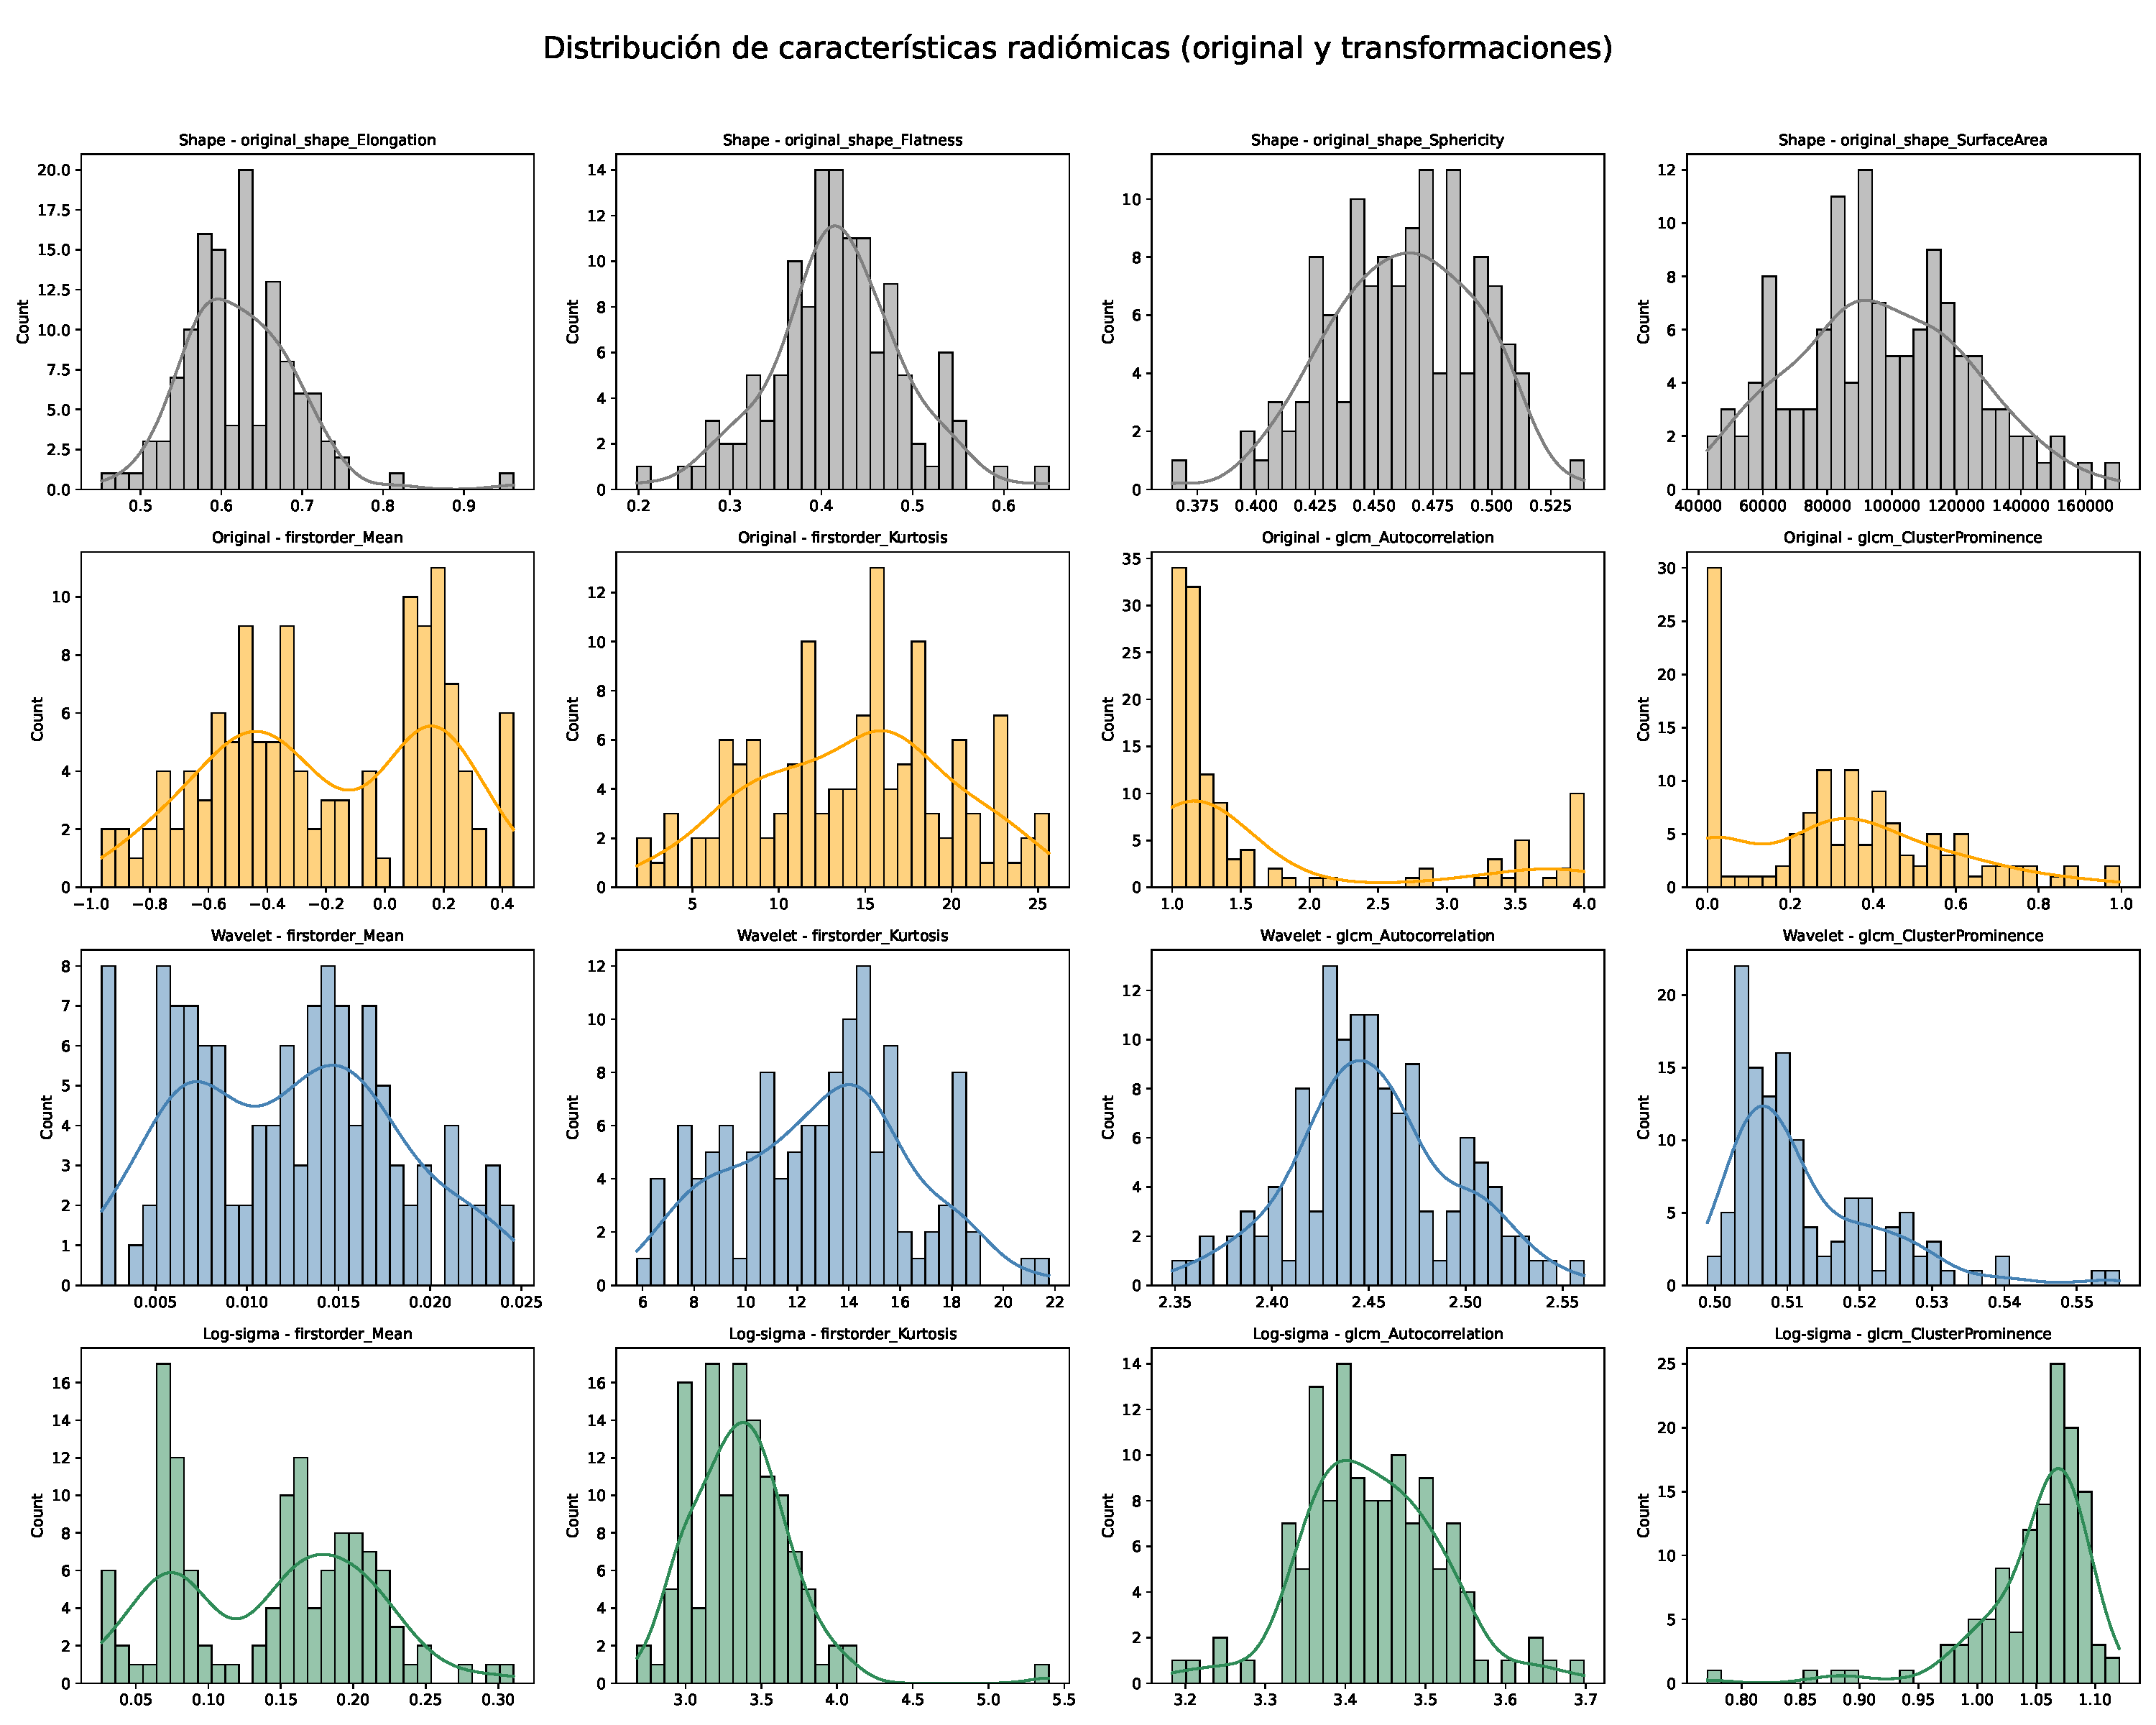
\includegraphics[width=\textwidth]{img/distribucion_features_radiomics.pdf}
\caption{Visualización de distribuciones de algunas características radiómicas. Se muestran tanto atributos de forma, como atributos sin transformar y los mismos atributos sobre las imágenes con filtros wavelet y logarítmicos.}\label{fig:dist_radiomics}
\end{figure}

Otro aspecto interesante a considerar es la correlación entre variables, ya que es posible que muchas características radiómicas estén altamente correlacionadas o incluso sean linealmente dependientes unas de otras. Puede ser el caso de ciertos percentiles de primer orden que se extraen, o ciertos atributos de las matrices de segundo orden. En la Figura \ref{fig:corr_radiomics} visualizamos la matriz de correlación de las características originales. Las extendidas no se muestran debido a su gran tamaño. Podemos observar que, efectivamente, hay muchas variables altamente correladas, tanto positiva como negativamente. Muchas de ellas, de hecho, alcanzan la correlación 1 o -1. No merece la pena tener tantas variables redundantes, así que se ha optado por eliminar, de todos los pares de atributos con correlación 1 o -1, uno de los pares, hasta que la matriz de correlación deje de tomar dichos valores. Se eliminan un total de 18 atributos redundantes entre las características originales, y un total de 585 al usar las características extendidas, dejando los datasets resultantes en unas dimensiones de $125 \times 89$, y $125 \times 1382$, respectivamente. En este último, la reducción es muy significativa, aunque aún sigue teniendo dimensionalidad muy alta. En la Figura \ref{fig:corr_after_remove} se muestra cómo queda la matriz de correlación tras eliminar todas las características redundantes. En ella podemos ver que las celdas con valores extremos disminuyen. Aun así quedan ciertos atributos altamente correlados sin llegar a ser dependientes. Por el momento, se ha optado por preservarlos.

\begin{figure}[!htbp]
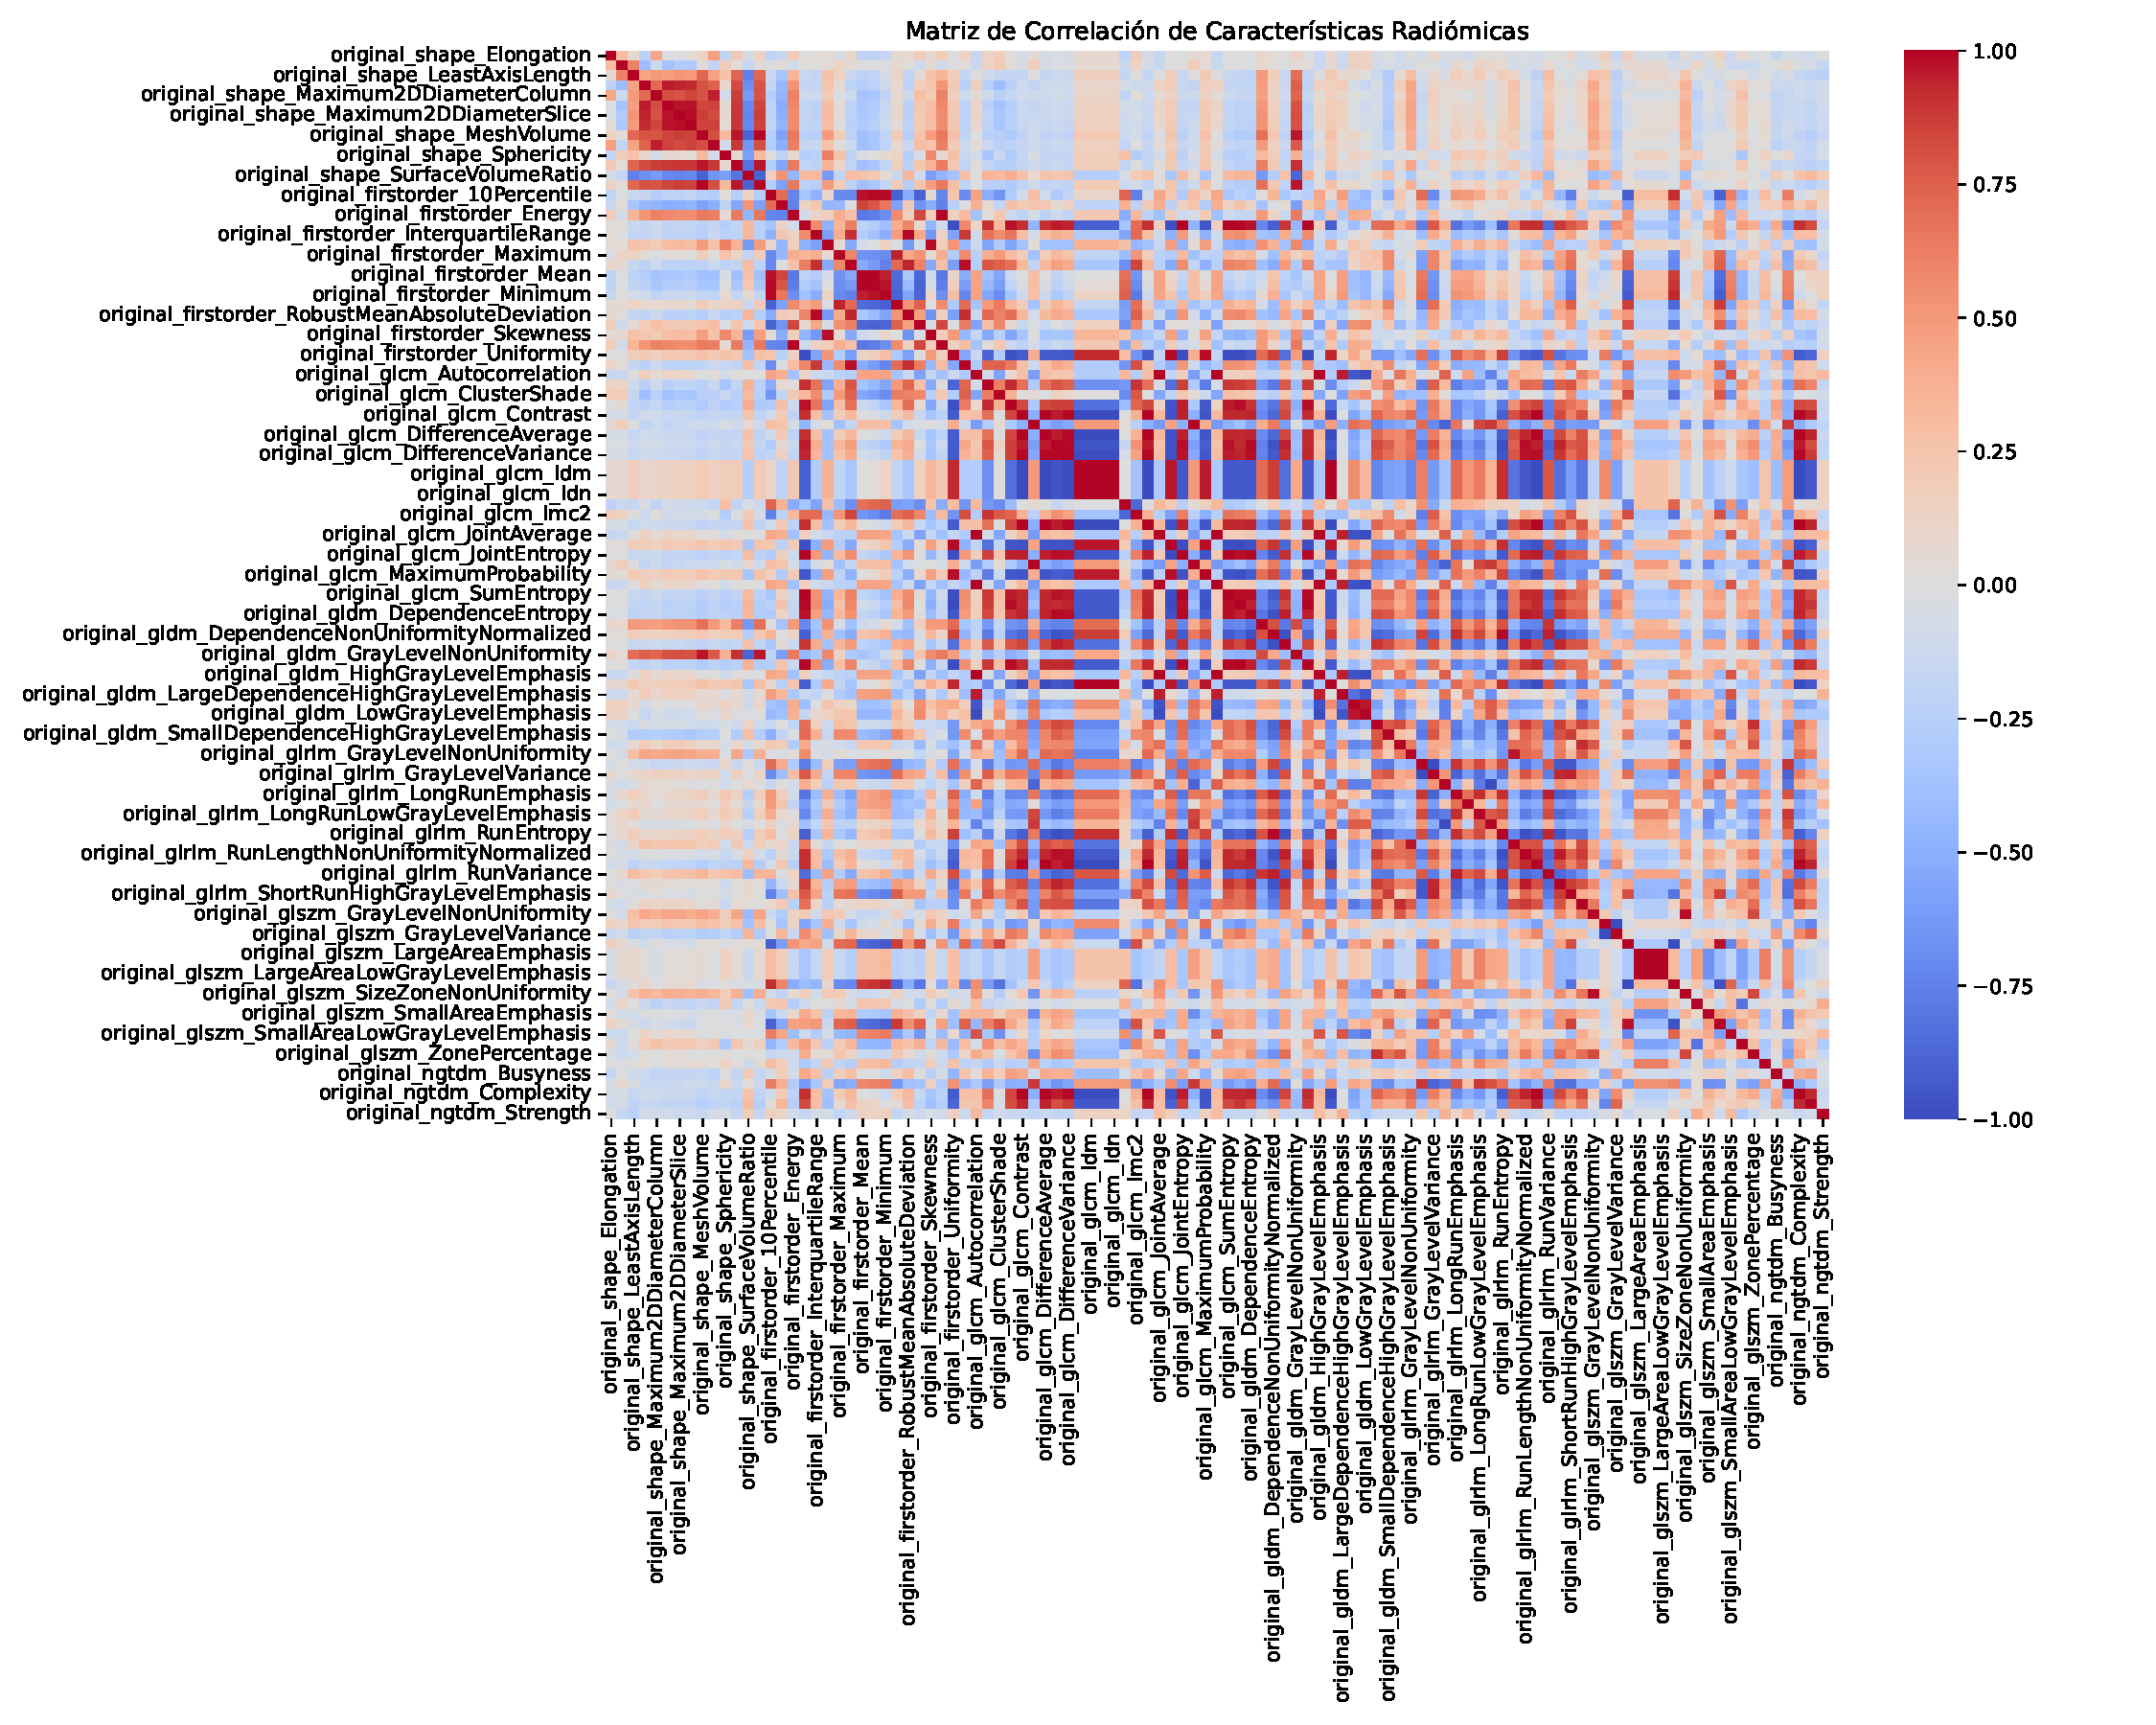
\includegraphics[width=\textwidth]{img/corrplot_radiomics.pdf}
\caption{Matriz de correlación sobre las características radiómicas originales.}\label{fig:corr_radiomics}
\end{figure}

\begin{figure}[!htbp]
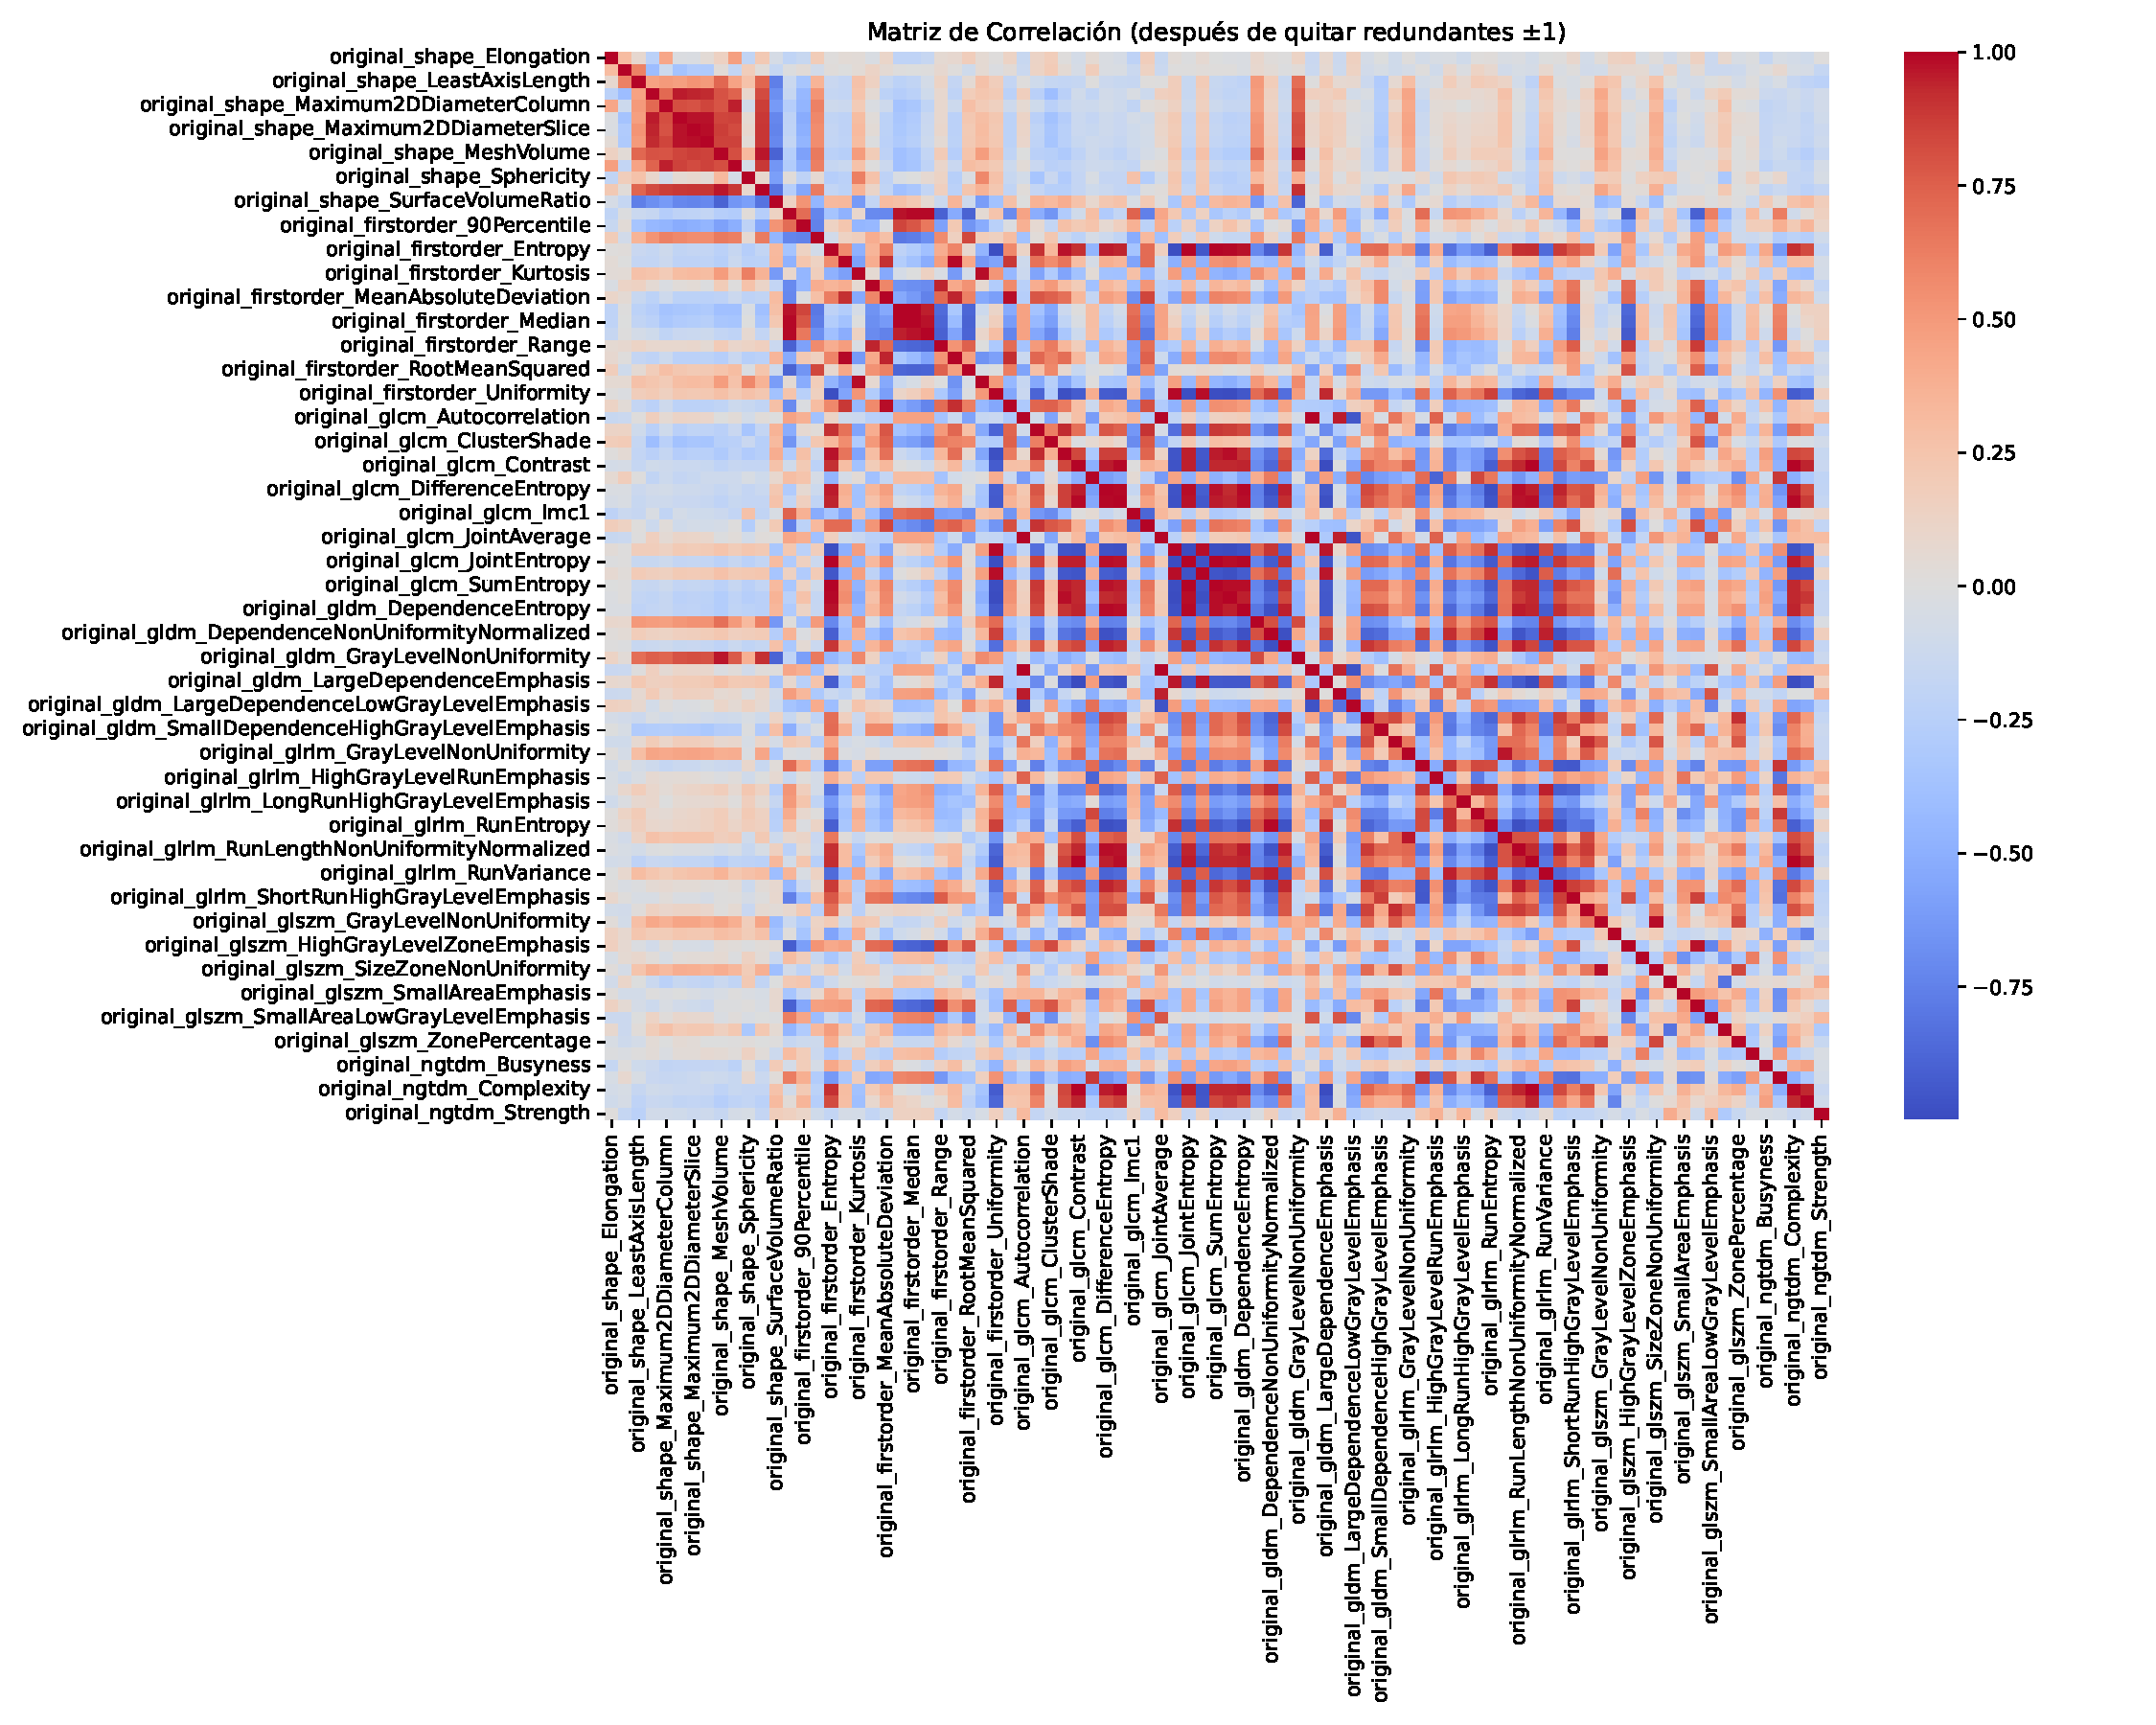
\includegraphics[width=\textwidth]{img/corrplot_radiomics_cleaned.pdf}
\caption{Matriz de correlación sobre las características radiómicas originales tras eliminar variables redundantes.}\label{fig:corr_after_remove}
\end{figure}

Otro aspecto interesante a tener en cuenta es el análisis de una posible correlación con las etiquetas, para tratar de identificar qué atributos pueden tener mayor influencia, individualmente, en la predicción de existencia de complicación. En las Figuras \ref{fig:corr_labels_original} y \ref{fig:corr_labels_extended} se muestran las características más correladas, en valor absoluto, con la etiqueta \emph{Complicación} de las características radiómicas, las originales y las extendidas, respectivamente. Tanto en las originales como en las extendidas, podemos ver que no destaca ninguna variable altamente correlada. En el caso de las extendidas, vemos que las características más correladas se corresponden casi todas con transformaciones \emph{wavelet} en diferentes direcciones, aunque apenas se llega a superar el 0.3 en el mejor caso. Por tanto, no parece que haya dependencias lineales con la clase que buscamos predecir y alguna característica individual.

% \begin{figure}[!htbp]
% \includegraphics[width=\textwidth]{top_features_corr_label_complicacion.pdf}
% \caption{Top 20 de características originales más correladas en valor absoluto con la existencia de complicación.}\label{fig:corr_labels_original}
% \end{figure}

% \begin{figure}[!htbp]
% \includegraphics[width=\textwidth]{ext_top_features_corr_label_tipo_complicacion.pdf}
% \caption{Top 20 de características extendidas más correladas en valor absoluto con la existencia de complicación.}\label{fig:corr_labels_extended}
% \end{figure}

\begin{figure}[!htbp]
    \centering
    \begin{subfigure}[t]{0.48\textwidth}
        \includegraphics[width=\textwidth]{img/top_features_corr_label_complicacion.pdf}
        \caption{Top 20 de características originales más correladas en valor absoluto con la existencia de complicación.}
        \label{fig:corr_labels_original}
    \end{subfigure}
    \hfill
    \begin{subfigure}[t]{0.48\textwidth}
        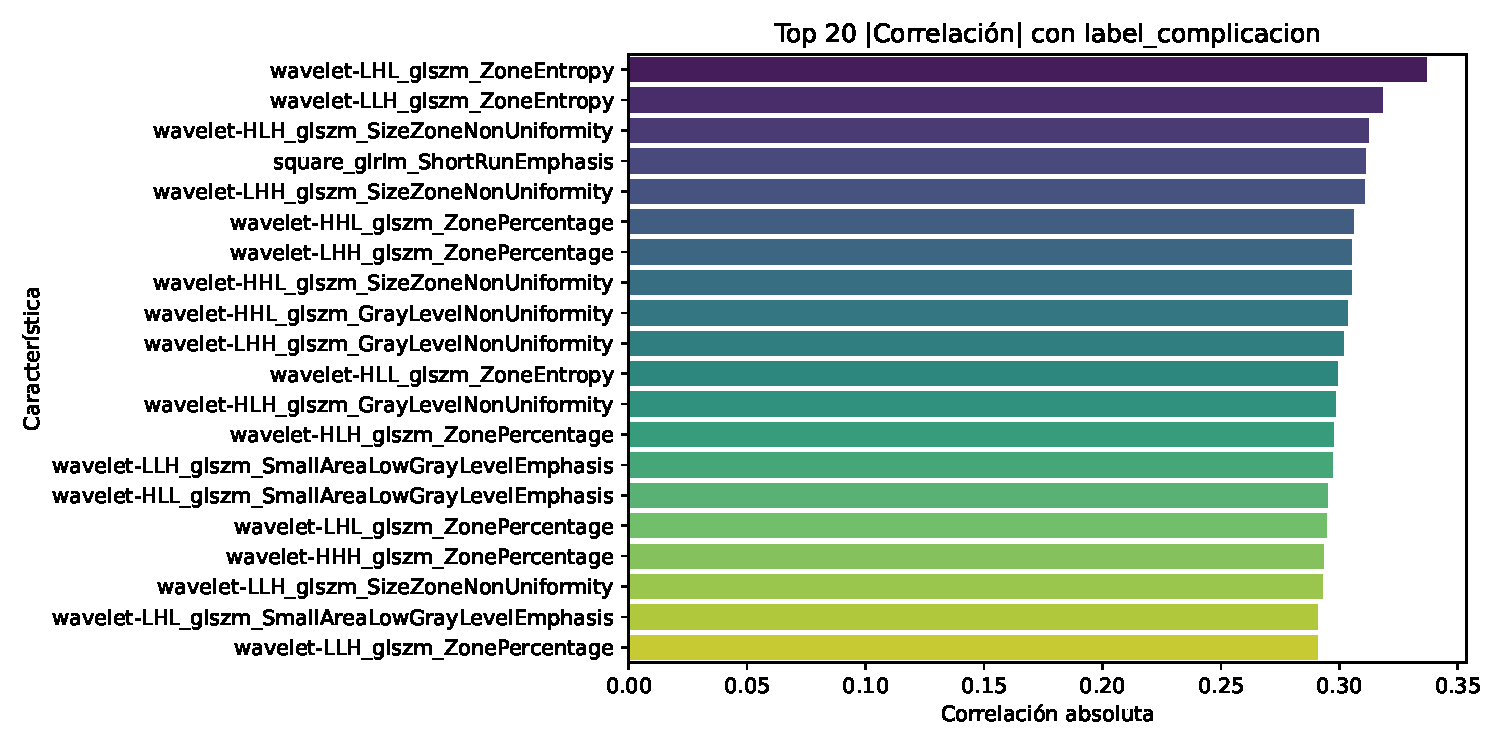
\includegraphics[width=\textwidth]{img/ext_top_features_corr_label_complicacion.pdf}
        \caption{Top 20 de características extendidas más correladas en valor absoluto con la existencia de complicación.}
        \label{fig:corr_labels_extended}
    \end{subfigure}
    \caption{Comparación de las 20 características más correladas con la existencia de complicación en el conjunto original (a) y extendido (b).}
    \label{fig:combined_corr_labels}
\end{figure}



Por último, dada la alta dimensionalidad presente en los datasets aún tras la eliminación de las variables redundantes, se ha optado por aplicar técnicas de selección de instancias y de reducción de dimensionalidad no supervisadas para la obtención de datasets de características más reducidos. Por un lado, se ha optado por aplicar la técnica de selección de características \emph{Variance Threshold}, que busca eliminar atributos con varianza inferior a un umbral pasado como parámetro. En nuestro caso, hemos tomado el umbral 0.01. Por otro lado, se ha utilizado \emph{PCA} como técnica de reducción de dimensionalidad, para obtener un mapeo en un espacio de menor dimensionalidad en el que se preserve la mayor parte de la varianza del dataset (se explican sus detalles en la Sección \ref{sec:pca}). En este caso, se ha optado por quedarse con varias posibilidades: el conjunto de componentes principales con las que se preserva el 99, 95 y 90 \% de la varianza, respectivamente. De cada posibilidad surge un dataset que se ha utilizado para entrenar los modelos de la siguiente sección. En la Tabla \ref{tbl:red_dim} se muestran las dimensionalidades alcanzadas tras aplicar estas técnicas (se muestran para el caso actual, para el resto de tamaños y ventanas el procedimiento es análogo y se consiguen resultados similares). Podemos ver que, especialmente, con las características extendidas, se reduce la dimensionalidad rápidamente, incluso con un PCA preservando el 99 \% de la varianza, lo que nos indica que puede que sea posible resumir la información de las características extendidas en 68 dimensiones sin perder demasiada información.

\begin{table}[!htbp]
\centering
\begin{tabular}{lcc}
\hline
 & \textbf{Original} & \textbf{Extendido} \\
\hline
Dimensión inicial       & 107 & 1967 \\
Sin redundantes         & 89  & 1382 \\
Variance Threshold      & 79  & 588  \\
PCA 99\%                 & 23  & 68   \\
PCA 95\%                 & 14  & 33   \\
PCA 90\%                 & 10  & 20   \\
\hline
\end{tabular}
\caption{Reducción de dimensionalidad para los conjuntos con características originales y extendidas obtenidas a partir del dataset de tamaño $128\times 256 \times 256$ sin aplicar ventanas Hounsfield.}
\label{tbl:red_dim}
\end{table}


\section{Entrenamiento de modelos de aprendizaje automático}

Finalmente, sobre los distintos datasets obtenidos con los procedimientos anteriores, se han probado distintos algoritmos de aprendizaje automático. Se han seleccionado algoritmos de diferente naturaleza para experimentar:

\begin{itemize}
    \item \textbf{Regresión logística.} Un algoritmo rápido y eficiente que, aunque en principio no se espera que logre buenos resultados, puede ayudar a hacernos una idea sobre la separabilidad lineal de los datos.
    \item \textbf{Árboles de decisión.} Otro algoritmo sencillo que posiblemente tampoco alcance buenos resultados, pero en caso afirmativo podría proporcionar interpretabilidad a los resultados.
    \item \textbf{SVM.} Las máquinas de vectores soporte son algoritmos robustos que además pueden adaptarse a distintas estructuras del conjunto de datos utilizando el kernel adecuado.
    \item \textbf{$k$-NN.} El algoritmo de los $k$ vecinos más cercanos puede ser efectivo si la representación espacial de los datos radiómicos es buena. Además, no tiene parámetros que aprender. Por otra parte, puede verse perjudicado especialmente por los conjuntos de datos de mayor dimensionalidad.
    \item \textbf{Ensembles.} Los ensembles suelen ser los algoritmos de aprendizaje automático clásico más efectivos en cuanto a capacidad de aprendizaje. Se ha optado por probar varios tipos de ensembles, tanto basados en bagging, como es el caso de los \emph{random forest}, como basados en boosting, para lo que se han seleccionado los algoritmos \emph{LightGBM}, \emph{XGBoost} y \emph{Gradient Boosting}.
\end{itemize}

El reducido número de instancias en nuestro conjunto de datos ha permitido la ejecución de múltiples versiones de los algoritmos variando parámetros. Por ejemplo, para el $k$-NN se han probado distintos números de $k$, en SVM distintos tipos de kernels y en los ensembles distinta cantidad de clasificadores débiles, entre otros. Los detalles de la experimentación se describirán en la Sección \ref{sec:experimentos}.

También es importante destacar que se ha experimentado con distintos tipos de normalización de los datos, previa a la ejecución de los algoritmos. Se han usado tanto la normalización estándar o Z-score, consistente en restar la media y dividir por la desviación típica, como la normalización \emph{MinMax}, que ajusta los rangos de todos los atributos al intervalo $[0, 1]$. La normalización es especialmente relevante en algoritmos basados en distancias, como el $k$-NN o las SVM.

Por último, se han probado dos modalidades de entrenamiento diferentes: entrenar solo con los datos radiómicos, y entrenar conjuntamente con los datos radiómicos y clínicos. En este último caso, los datos clínicos se incorporan al conjunto de radiómicos antes de realizar las normalizaciones de los datos, para que atributos como la edad del paciente sean normalizados posteriormente, y todas aquellas características clínicas nominales que numerizan con un \emph{one-hot encoding}.

\section{Aprendizaje de métricas de distancia}

Para concluir este capítulo, nos centramos en un caso especial observado durante los resultados de las experimentaciones anteriores. Estos resultados se pueden consultar en la Sección \ref{sec:resultados}. En dicha sección, se puede observar que el $k$-NN, junto con los ensembles, es el algoritmo que más destaca, obteniendo algunos de los mejores resultados. Dichos resultados se obtienen usando la distancia euclídea, que es una distancia estándar que considera a todos los atributos con la misma importancia. Por ello, nos planteamos el intentar mejorar estos resultados aprendiendo una distancia a partir de los datos, y usar dicha distancia posteriormente en el $k$-NN.

Para ello, recurrimos a las técnicas de aprendizaje de métricas de distancia descritas en la Sección \ref{sec:dist}. Concretamente, aplicaremos los siguientes algoritmos LMNN y NCA. Ambos algoritmos están diseñados específicamente para mejorar el rendimiento del $k$-NN, y las transformaciones que aprenden pueden utilizarse para definir una reducción de dimensionalidad con información supervisada, a diferencia de las técnicas aplicadas anteriormente. 

Ambos algoritmos se han aplicado a los conjunto de características originales eligiendo distintos valores como dimensión de salida: 10, 20, 30 y la dimensión completa. Con ello se ha buscado obtener nuevas representaciones del conjunto de datos en las que el algoritmo $k$-NN pudiera alcanzar un mayor rendimiento, y así superar el mejor resultado global alcanzado en este problema.

Al igual que en el entrenamiento sin aprendizaje de métricas de distancias, también se prueba en este caso la incorporación de los datos clínicos. En este caso, los datos se incorporan antes del aprendizaje de las distancias, para que se vean afectados también por la transformación que aprendan los algoritmos.

\endinput
%--------------------------------------------------------------------
% FIN DEL CAPÍTULO. 
%--------------------------------------------------------------------

% !TeX root = ../tfg.tex
% !TeX encoding = utf8

\chapter{Análisis experimental} \label{analisis-resultados}

En este capítulo se presenta la experimentación realizada, los resultados obtenidos y el análisis detallado de los resultados obtenidos tras entrenar y validar los modelos desarrollados para predecir complicaciones en biopsias pulmonares. Se describen las métricas utilizadas para evaluar el desempeño, así como las estrategias de validación empleadas para garantizar la robustez de los resultados.  

Aunque el objetivo final de esta línea de investigación es desarrollar modelos capaces de predecir no solo la existencia de complicaciones, sino también el tipo específico de riesgo (como neumotórax, hemorragia u otros riesgos), en este trabajo se ha optado por abordar primero la tarea de clasificación binaria (complicación: sí/no). Esta decisión se tomó tras valorar las limitaciones del conjunto de datos disponible y comprobar que los resultados para la tarea binaria ya planteaban un reto considerable. De este modo, se priorizó consolidar un modelo sólido para la predicción general de complicaciones, como paso previo indispensable para avanzar hacia la clasificación más detallada por tipos de riesgo en futuros trabajos.  

A continuación, se exponen los distintos experimentos realizados, destacando las configuraciones adoptadas y las variantes comparadas (modelos 2D y 3D, estrategias de preentrenamiento, integración de datos clínicos, radiómica). Finalmente, se analizan textualmente los resultados obtenidos tanto en validación como en test con un análisis cualitativo.

\section{Métricas y métodos de validación usados}

\subsection{Métricas}

Para evaluar el rendimiento de los modelos desarrollados se emplearon varias métricas estándar en problemas de clasificación binaria. A continuación se detallan las principales métricas utilizadas, su interpretación y su relevancia en el contexto del problema.

En primer lugar, para poder calcular estas métricas, es necesario definir los conceptos básicos:

\begin{itemize}
    \item $TP$ (True Positives, verdaderos positivos): número de casos en los que el modelo predijo correctamente la clase positiva. En nuestro contexto, corresponde a pacientes correctamente identificados como con complicación.
    \item $TN$ (True Negatives, verdaderos negativos): número de casos en los que el modelo predijo correctamente la clase negativa. Es decir, pacientes correctamente identificados como sin complicación.
    \item $FP$ (False Positives, falsos positivos): número de casos en los que el modelo predijo erróneamente la clase positiva. Son pacientes sin complicación que fueron clasificados como con complicación.
    \item $FN$ (False Negatives, falsos negativos): número de casos en los que el modelo predijo erróneamente la clase negativa. En este caso, pacientes con complicación que fueron clasificados como sin complicación.
\end{itemize}

Definidos estos términos, la \textbf{matriz de confusión} ofrece una representación tabular que sintetiza esta información. Sirve para comprender mejor la calidad de las predicciones. En nuestro caso, este análisis permitió identificar patrones de error sistemático, como la tendencia del modelo a fallar más en la detección de la clase minoritaria.
   

\begin{itemize}
    \item El \textbf{Accuracy} o exactitud mide el porcentaje de predicciones correctas sobre el total de instancias. Es una métrica intuitiva y sencilla que ofrece una visión global del rendimiento del modelo:

    \[
    \text{Accuracy} = \frac{TP + TN}{TP + TN + FP + FN}
    \]

    Sin embargo, el accuracy puede ser engañoso en contextos con clases desbalanceadas. Por ejemplo, en un conjunto de datos donde la mayoría de los pacientes no presentan complicaciones, un modelo que siempre predice \textit{sin complicación} puede alcanzar una accuracy elevada sin identificar adecuadamente los casos de riesgo.

\end{itemize}

Para analizar con mayor detalle el comportamiento del modelo se emplean métricas que permiten evaluar de forma separada su rendimiento en la identificación de la clase positiva (complicación) y de la clase negativa (sin complicación):

\begin{itemize}
    \item \textbf{Precisión} (\textit{Precision}): mide la proporción de predicciones positivas que son correctas, es decir, cuántos de los pacientes clasificados como con complicación realmente presentan dicha complicación. Se define como:

    \[
    \text{Precision} = \frac{TP}{TP + FP}
    \]

    Una precisión alta implica que el modelo comete pocos falsos positivos.

    \item \textbf{Sensibilidad} o \textbf{True Positive Rate (TPR)} (\textit{Recall}): cuantifica la capacidad del modelo para identificar correctamente las instancias positivas. En nuestro contexto, mide cuántos pacientes con complicación son efectivamente detectados por el modelo. Se calcula como:

    \[
    \text{Recall} = \text{TPR} = \frac{TP}{TP + FN}
    \]

    Una sensibilidad elevada es esencial en aplicaciones médicas, ya que reduce el riesgo de pasar por alto casos que requieren atención.

    \item \textbf{Especificidad} o \textbf{True Negative Rate (TNR)}: evalúa la proporción de instancias negativas correctamente identificadas. En este problema, refleja la capacidad del modelo para reconocer correctamente a los pacientes que no presentan complicación. Se define como:

    \[
    \text{Specificity} = \text{TNR} = \frac{TN}{TN + FP}
    \]

    Una alta especificidad evita falsos positivos, reduciendo alarmas innecesarias y optimizando el uso de recursos médicos.
\end{itemize}

Estas métricas son complementarias y fundamentales para entender el comportamiento del modelo de forma equilibrada, ya que permiten evaluar tanto la detección efectiva de los casos de complicación como la capacidad de evitar clasificaciones erróneas en pacientes sanos.

\begin{itemize}
    \item \textbf{F1-score}: combina precisión y recall en una media armónica, ofreciendo un equilibrio entre ambas métricas.

    \[
    F1 = 2 \times \frac{\text{Precision} \times \text{Recall}}{\text{Precision} + \text{Recall}}
    \]

    El F1-score es especialmente útil cuando hay un desbalance entre clases, ya que penaliza los casos en los que una de las métricas es mucho más baja que la otra. Sin embargo, durante el análisis se observó que en algunos casos, debido al fuerte desbalance de clases, el modelo podía alcanzar valores relativamente altos de F1-score simplemente favoreciendo sistemáticamente la clase mayoritaria, es decir, hacia la no complicación". Esto evidenció la necesidad de utilizar métricas adicionales que evaluaran de forma más equilibrada ambas clases.

    \item \textbf{GMean}: para abordar de forma más directa el problema del desbalance de clases, se empleó la métrica G-Mean o media geométrica de la sensibilidad (recall) y la especificidad. El G-Mean se calcula como:

    \[
    \text{G-Mean} = \sqrt{\text{Recall} \times \text{Specificity}}
    \]

    Esta métrica penaliza las soluciones que favorecen en exceso la clase mayoritaria y permite evaluar la capacidad del modelo para identificar correctamente ambas clases de forma equilibrada. Por este motivo, se adoptó el G-Mean como criterio principal de selección de modelos, ya que reflejaba mejor la capacidad del sistema para discriminar entre pacientes con y sin complicaciones, incluso en presencia de datos desbalanceados. Además, tiene la ventaja de que permite detectar fácilmente modelos triviales que predicen todo como una única clase: en esos casos, la sensibilidad o la especificidad se anulan, haciendo que el valor del G-Mean sea 0.


\end{itemize}





\subsection{Métodos de validación}

A lo largo del desarrollo del proyecto se fueron adaptando diferentes estrategias de validación para evaluar el rendimiento de los modelos de manera cada vez más robusta, siguiendo una progresión acorde con el aprendizaje obtenido sobre las limitaciones del problema y el propio dataset.

En las primeras fases, se empleó el esquema más sencillo: \textit{hold-out} sin estratificar. En este enfoque, se dividió el conjunto de datos en dos particiones (entrenamiento y test) con distintas proporciones de split (por ejemplo, 80\%-20\% o 70\%-30\%), utilizando la porción de entrenamiento para ajustar el modelo y la de test para evaluar su capacidad de generalización. Esta técnica es sencilla y rápida computacionalmente, pero tiene el inconveniente de que no aprovecha todos los datos para el entrenamiento y su resultado puede depender mucho de la partición elegida, especialmente en datasets reducidos.

Al detectar problemas de \emph{desbalanceo de clases} en el conjunto de datos se pasó a realizar \textit{hold-out estratificado}. El objetivo era preservar en ambos conjuntos la proporción original de las clases, evitando que el modelo entrenara o se evaluara sobre distribuciones sesgadas.

No obstante, dada la reducida cantidad de muestras, se consideró necesario utilizar metodologías que aprovecharan mejor la información disponible. Por ello, se adoptó el uso de \textit{validación cruzada estratificada} (\emph{stratified cross-validation}), que asegura la misma proporción de clases en cada fold. Este método divide los datos en \(k\) particiones aproximadamente del mismo tamaño y proporción de clases, entrenando el modelo \(k\) veces con \(k-1\) folds para entrenamiento y 1 para validación en cada iteración. Para este trabajo se probaron distintos valores de \(k\), incluyendo \(k=5\) y \(k=10\), que ofrecían un buen compromiso entre estabilidad estadística y coste computacional.

En el caso concreto de los experimentos con cortes 2D, donde el número de pacientes se traduce en un mayor número de slices pero el problema de variabilidad entre ellos es mayor, se exploró también la estrategia de \textit{leave-one-out cross-validation}. En este enfoque extremo de \(k\)-fold, en cada iteración se usa un único paciente como test y todos los demás para entrenar. Esta técnica permite aprovechar casi todos los datos para el entrenamiento en cada ciclo y es especialmente útil en conjuntos pequeños. Sin embargo, debido a su elevado coste computacional y a que no mejoró de forma consistente el rendimiento, se descartó.

Finalmente, como método de validación principal y definitivo, se implementó un esquema de validación cruzada estratificada con \(k=5\) folds, incluyendo además un \emph{split} interno del conjunto de entrenamiento en cada fold. En este enfoque, el conjunto de datos se divide primero en un 80\% para entrenamiento y validación y un 20\% reservado como test que nunca ve los datos durante el entrenamiento. Posteriormente, en cada fold de entrenamiento y validación, se realiza una segunda división interna (80\% para entrenar y 20\% para validar), usando la partición de validación para hacer \emph{early stopping} y guardar el mejor modelo. Una vez finalizado el entrenamiento, el mejor modelo se evalúa en el conjunto de test correspondiente, que permaneció completamente aislado. Este esquema más elaborado y cuidadoso asegura una estimación más fiable del rendimiento en datos no vistos, equilibrando el uso eficiente de los datos limitados con la necesidad de evitar sobreajuste.




\section{Descripción de los experimentos} \label{sec:experimentos}

A continuación se describen de forma ordenada y temporal los diferentes experimentos realizados en este trabajo. Todos estos experimentos se fueron planteando progresivamente para abordar el tamaño reducido del dataset, el desbalanceo de clases, la complejidad de las imágenes 3D y la falta de literatura previa que indicara las mejores estrategias. 


\subsection{Experimentos preliminares}
En esta fase inicial se realizaron pruebas con los datos disponibles en cada momento. Dado que el conjunto de datos fue aumentando progresivamente a medida que avanzaba la recopilación, los experimentos preliminares no siempre contaron con los 125 pacientes finales. Estas primeras pruebas sirvieron para validar la viabilidad del enfoque, ajustar la arquitectura del modelo y orientar las decisiones posteriores.


\subsubsection{Modelos basados en imágenes 2D.} 
Se comenzó probando un enfoque 2D, donde se entrenaban modelos con slices de los volúmenes TC. Se empleó \textit{EfficientNetV2-S} preentrenada en ImageNet, modificando la primera capa para un solo canal y la última para clasificación binaria. Inicialmente se entrenó congelando todas las capas menos la última, usando BCE Loss y el optimizador Adam con $lr=0.001$. Aunque en entrenamiento la pérdida bajaba algo, en validación permanecía muy alta, con F1-scores cercanos a cero, indicando un mal rendimiento. Posteriormente se realizaron ajustes finos (\emph{fine-tuning}) con learning rates más bajos y weight decay, obteniendo ligeras mejoras en entrenamiento pero sin mejoras reales en validación.

Para reducir el sesgo por la selección del split, se pasó a usar \textit{cross-validation estratificado (k=5)} agrupado por paciente porque si no habría fuga de información, para garantizar que las slices de un paciente concreto no aparecieran en entrenamiento y test simultáneamente. También se probó con \textit{leave-one-out} cuando el número de pacientes era muy reducido (55 pacientes), pero en todos los casos el F1-score en test se mantuvo muy bajo. Finalmente, se exploraron estrategias de \textit{preentrenamiento} usando datasets públicos de pulmones (como Lung-PET-CT-Dx \parencite{lungPetCtDx}), aplicando early stopping y fine-tuning, pero los resultados siguieron sin ser satisfactorios. Por las limitaciones propias de clasificar slices 2D, como la gran variabilidad entre cortes de un mismo volumen (con slices extremas sin información relevante) y el fuerte aumento del desbalanceo al dividir en cortes, esta aproximación fue finalmente descartada.



\subsubsection{Experimentos con datos 3D}

Una vez descartada la aproximación basada en cortes 2D, el trabajo se centró en entrenar modelos 3D directamente sobre los volúmenes completos de TC de nuestro propio dataset. Aquí se detallan las principales configuraciones y resultados obtenidos.

En las primeras fases se emplearon volúmenes originales (sin segmentación) con resoluciones elevadas, como $(256, 512, 512)$ o  $(128,256,256)$, y un \textit{batch size} de 1 debido a las limitaciones de memoria del servidor. Se utilizó una partición \textit{hold-out} sin estratificar, aplicando la función de pérdida CrossEntropyLoss. Los resultados mostraron que la pérdida bajaba muy poco y las métricas eran nulas (Accuracy: 0.6364, F1 Score: 0.0000), con una matriz de confusión que indicaba que el modelo predecía sistemáticamente la clase mayoritaria.

Para intentar contrarrestar este efecto, se aplicó una ponderación de clases en la función de pérdida, asignando mayor peso a la clase minoritaria. Sin embargo, esto no mejoró el problema, manteniéndose la predicción constante en la clase mayoritaria y el F1 en cero.

Posteriormente se incorporó \texttt{WeightedRandomSampler} para duplicar las instancias de la clase minoritaria en entrenamiento. Se experimentó con diferentes potencias (power) para incrementar el efecto del muestreo. Además, se introdujo dropout y se probó con la función de pérdida \textit{focal loss} con parámetros $\alpha=0.9$, $\gamma=1.8$, usando el optimizador AdamW con $lr=1e^{-4}$ y $weight\_decay=1e^{-5}$ junto a un scheduler ReduceLROnPlateau. A pesar de estas estrategias, la pérdida no convergía bien con los siguientes resultados: en entrenamiento (Accuracy: 0.6462, F1 Score: 0.7850) y en validación (Accuracy: 0.2857, F1 Score: 0.4444).

Aumentando la potencia del sampler se forzaba demasiado la clase minoritaria, logrando en entrenamiento un F1 alto (0.8491), pero en validación seguía siendo bajo y la matriz de confusión mostraba que el modelo predecía casi siempre la clase minoritaria. 

También se aplicó generación sintética de la clase minoritaria mediante transformaciones como \texttt{RandFlip}, \texttt{RandAffine} y \texttt{RandGaussianNoise}, combinadas con el WeightedRandomSampler, Adam y CrossEntropyLoss con ReduceLROnPlateau. No obstante, los resultados mostraron que el modelo no lograba aprender patrones discriminativos sólidos: loss de validación: 6.16, Accuracy: 0.6250 y F1 Score: 0.0000. Es decir, todo lo clasificaba como la clase mayoritaria. 

Además, se exploró el uso de preentrenamiento en conjuntos de datos 3D externos para transferir conocimiento al problema objetivo. La idea era inicializar el modelo con pesos aprendidos en tareas similares, esperando que esto mejorara la capacidad de generalización dadas las limitaciones de tamaño de nuestro dataset. Por tanto, se realizó un preentrenamiento usando un dataset 3D público y genérico, con imágenes de TC y tareas de clasificación anatómica. Los resultados de este preentrenamiento alcanzaron una Accuracy de 0.6108 y un F1-score de 0.6335 en la tarea fuente. Sin embargo, al aplicar Grad-CAM para analizar las activaciones, se observó que el modelo tendía a fijarse en regiones fuera del pulmón o incluso en toda la imagen de forma difusa, evidenciando que no aprendía características relevantes para la predicción de complicaciones pulmonares.

Tras el preentrenamiento, se realizó un ajuste fino (fine-tuning) en nuestro dataset con DenseNet121 como arquitectura base, incorporando WeightedRandomSampler para mitigar el desbalanceo de clases y usando CrossEntropyLoss. El entrenamiento se realizó con el optimizador Adam. Los resultados mostraron una Accuracy de 0.6287 y un F1-score de 0.6438. Sin embargo, Grad-CAM seguía señalando regiones externas al pulmón o activaciones muy dispersas, sin focalización en estructuras anatómicamente coherentes.

A continuación, se implementó un esquema de validación hold-out estratificado (85/15) para mantener la proporción de clases, entrenando DenseNet121 sin dropout y congelando todas las capas salvo la final. Se utilizó de nuevo CrossEntropyLoss y Adam. En este escenario, la función de pérdida en entrenamiento apenas descendía y los resultados fueron: Training Accuracy 0.6885, F1-score 0.5615, mientras que en validación se obtuvo Val Loss 7.4704, Accuracy 0.7273 y F1-score 0.7080. A pesar del valor relativamente alto de F1 en validación, la matriz de confusión mostró que el modelo predecía sistemáticamente la clase mayoritaria.

Finalmente, se probó descongelar parcialmente algunas capas intermedias para permitir una mayor adaptación del modelo, utilizando un learning rate reducido de $1\times 10^{-5}$. Los resultados en entrenamiento fueron similares (Accuracy 0.6885, F1-score 0.5615), mientras que en validación la pérdida bajó ligeramente (6.8962), con Accuracy 0.7273 y F1-score 0.6124. Sin embargo, el análisis de Grad-CAM seguía mostrando patrones sin sentido clínico, activándose en regiones irrelevantes y confirmando que el modelo no lograba aprender características discriminativas reales sin segmentación pulmonar previa.

Al ver los malos resultados, se aplicaron técnicas de explicabilidad para intentar entender por qué el modelo no funcionaba y nos dimos cuenta en que solo se centraba en regiones fuera del pulmón, por lo que vimos esencial segmentar pulmones para seguir con la investigación. 


Una técnica clave fue incorporar \textit{segmentación pulmonar} en el preprocesamiento, aislando solo los pulmones y eliminando regiones irrelevantes. Se entrenaron tanto ResNet3D como DenseNet121 sobre estos volúmenes segmentados.

Por ejemplo, usando ResNet se obtuvieron resultados como: Training Loss: 50.47, Acc: 0.67, F1: 0.59, con Validation Loss: 9.18, Acc: 0.71 y F1: 0.50, mostrando cierta mejora en balancear clases (G-Mean: 0.5774). 

Probando ResNet sin aplicar ventanas HU se alcanzó un ajuste casi perfecto en entrenamiento (F1: 1.00) pero validación más razonable (Acc: 0.61, F1: 0.58, G-Mean: 0.61).

Por último, entrenando DenseNet121 con alrededor de 100 pacientes y utilizando \textit{acumulación de gradiente} (virtual batch size mayor ya que por memoria no podíamos utilizar un batch size mayor) se consiguieron los mejores resultados en validación: Training Acc: 0.89, F1: 0.88, Validation Acc: 0.75, F1: 0.67 y G-Mean: 0.71. Esto sugiere que la combinación de segmentación, un diseño 3D adecuado y técnicas para simular batch grandes fueron claves para mejorar el rendimiento con datos limitados.

Una vez incorporada la segmentación pulmonar al preprocesamiento, se exploraron dos estrategias de preentrenamiento distintas.

En esta estrategia, se realizó primero un preentrenamiento supervisado usando un conjunto de datos 3D público de pulmones y posteriormente se aplicó fine-tuning en nuestro propio conjunto de datos segmentado.

En entrenamiento, los resultados fueron prometedores, alcanzando una pérdida de 4.3998, Accuracy de 83.93\%, F1-score de 0.6897 y un G-Mean de 0.7603. Sin embargo, en validación los resultados se degradaron notablemente, con una Loss muy alta (28.5546) y un F1-score de 0.0000. El análisis de la matriz de confusión mostró que el modelo caía en la predicción total hacia la clase mayoritaria. A pesar de la segmentación, el preentrenamiento genérico no logró transferir conocimiento útil para la tarea objetivo, probablemente por ser otro problema, predicción de cáncer pulmonar.

Para mitigar el problema del desbalanceo de clases en el fine-tuning, se incorporó un esquema de \texttt{WeightedRandomSampler} y se utilizó \textit{Focal Loss}, que penaliza más los ejemplos difíciles de clasificar, combinado con \textit{Early Stopping} para evitar sobreajuste. Sin embargo, tampoco mejoro el rendimiento en general. 

\subsection{Experimentos finales}

Se han realizado tres ramas principales de experimentos con el conjunto final de datos del proyecto:

\begin{itemize}
    \item \textbf{Cross-validation con diferentes configuraciones}: experimentos sistemáticos con validación cruzada con 5 folds con el modelo DenseNet121, variando parámetros clave del entrenamiento.
    \item \textbf{Imágenes con datos clínicos}: integración multimodal que combina volúmenes TC segmentados con variables clínicas tabulares del paciente.
    \item \textbf{Preentrenamiento y fine-tuning con MedMNIST3D}: transferencia de aprendizaje usando un dataset abierto para inicializar pesos y afinar después en nuestro conjunto específico.
    \item \textbf{Aprendizaje automático clásico con datos clínicos}: modelos tradicionales entrenados solo con variables tabulares para evaluar su rendimiento y compararlo con el enfoque basado en imágenes.
    \item \textbf{Radiómica}: extracción de características cuantitativas de las imágenes TC para construir modelos predictivos con métodos clásicos de machine learning.
\end{itemize}


Para todos los experimentos finales se utilizó un mismo \textit{pipeline} con validación cruzada estratificada (\( k=5 \) folds) con siempre las mismas particiones para evaluar y poder comparar los modelos. En el entrenamiento de los datos volumétricos con deep learning se exploraron distintas configuraciones:

\begin{itemize}
    \item \textbf{Preprocesamiento}: diferentes ventanas de Hounsfield: de centro -600 y anchura 1500 ([-1350,150]) y de centro -300 y anchura 1400 ([-1000,400]) y sin ventana. Además, diferentes tamaños de volúmenes: (64,64,64), (128,128,128) y (128,256,256).
    \item \textbf{Batch sizes variados}: se compararon tamaños de batch como 2, 4, 8, 16 y 32, teniendo en cuenta limitaciones de memoria GPU y el tamaño del dataset.
    \item \textbf{Parámetros de optimización}: se usó el optimizador Adam con diferentes valores de \texttt{learning rate}, \texttt{weight decay} y probabilidad de \texttt{dropout} para regularizar el modelo y reducir el sobreajuste.
    \item \textbf{Scheduler de learning rate}: en algunos experimentos se incluyó un ajuste dinámico del \texttt{learning rate} mediante estrategias como \texttt{CosineAnnealing} o \texttt{ReduceLROnPlateau}, para facilitar una convergencia más estable en fases avanzadas del entrenamiento. En otros, dejamos la tasa de aprendizaje fija. 
\end{itemize}
  
Tras comprobar que los resultados obtenidos con modelos de deep learning no alcanzaban el rendimiento esperado, se consideró que este enfoque no siempre es la única opción, especialmente en escenarios con cantidades de datos limitadas. El aprendizaje profundo requiere habitualmente grandes volúmenes de datos para generalizar correctamente, por lo que la baja disponibilidad de pacientes en nuestro caso podía explicar en parte el rendimiento insuficiente.  

Por este motivo, se decidió explorar técnicas más clásicas de aprendizaje automático, que suelen ser más robustas en contextos con datos más reducidos. Para ello, se realizaron experimentos utilizando exclusivamente datos tabulares clínicos, empleando los siguientes algoritmos: \texttt{KNN}, \texttt{Random Forest}, \texttt{LightGBM}, \texttt{XGBoost}.  


En la parte del estudio de la radiómica, se extrajeron características cuantitativas de las imágenes TC segmentadas para construir modelos predictivos sobre datos tabulares derivados de la imagen. Se definieron cuatro grandes combinaciones experimentales para analizar el efecto de distintas fuentes de información y técnicas de representación:

\begin{itemize}
    \item \textbf{Sin datos clínicos ni DML}: modelos basados exclusivamente en radiómica pura, evaluando distintas estrategias de selección de características, escalado y reducción de dimensionalidad. Incluye los clasificadores indicados arriba, y además se hicieron pruebas también con árboles de decisión.
    \item \textbf{Con datos clínicos y sin DML}: integración de variables clínicas junto con las características radiómicas, para evaluar la aportación de la información del paciente al modelo final. Se utilizan los mismos clasificadores.
    \item \textbf{Sin datos clínicos y con DML}: aplicación de técnicas de metric learning (como NCA y LMNN) con reducción de dimensionalidad a distintos tamaños para aprender representaciones más discriminativas del espacio radiómico, incluso sin disponer de datos clínicos adicionales.
    \item \textbf{Con datos clínicos y con DML}: combinación más completa, integrando datos clínicos con técnicas de metric learning sobre radiómica, con el objetivo de explotar al máximo la complementariedad entre la información anatómica de imagen y los factores clínicos del paciente. Se evalúan solo con el KNN.
\end{itemize}

Para cada algoritmo, se ha realizado una grid search para estimar los parámetros relevantes para el aprendizaje más apropiados:

\begin{itemize}
    \item \textbf{Árboles de decisión:} profundidad máxima del árbol (\texttt{max\_depth}) y mínimo número de ejemplos para dividir un nodo \texttt{min\_samples\_split}.
    \item \textbf{SVM:} tipo de kernel (\texttt{kernel}), regularización (\texttt{C}) y coeficiente del kernel (\texttt{gamma})
    \item \textbf{$k$-NN:} número de vecinos (\texttt{n\_neighbors}) y cómo ponderar los pesos de cada vecino (\texttt{weights})
    \item \textbf{Ensembles:} Número de estimadores débiles (\texttt{n\_estimators}) y, según el caso, tasa de aprendizaje (\texttt{learning\_rate}) o los parámetros de árbol descritos en el árbol de decisión.
\end{itemize}

El objetivo fue determinar hasta qué punto la inclusión de datos clínicos y el uso de metric learning podían mejorar el rendimiento respecto a la radiómica pura, observándose finalmente que la combinación de ambas estrategias ofrecía los mejores resultados globales.







\begin{table}[!htbp]
\centering
\caption{Resultados medios con DenseNet121 en test y validación con validación cruzada con k=5. Ordenados por G-Mean.}
\label{tab:resultados-crossvalidate}
\resizebox{\textwidth}{!}{%
\begin{tabular}{lcccccccccccc}
\toprule
\textbf{Set} & \textbf{Batch Size} & \textbf{LR} & \textbf{Weight Decay} & \textbf{Dropout} & \textbf{Preprocesado} & \textbf{Accuracy} & \textbf{F1} & \textbf{TPR} & \textbf{TNR} & \textbf{G-Mean} \\
\midrule
TEST  & 4 & 0.001 & 0 & 0.3 & (64,64,64) HU [-1000,400] & 0.696 & 0.680 & 0.679 & 0.709 & 0.691 \\
VALIDATION  & 4 & 0.001 & 0 & 0.3 & (64,64,64) HU [-1000,400] & 0.720 & 0.697 & 0.720 & 0.722 & 0.715 \\
\midrule
TEST &  16 & 0.001 & 0 & 0.4 & (64,64,64) HU [-1000,400] & 0.680 & 0.687 & 0.747 & 0.619 & 0.674 \\
VALIDATION  & 16 & 0.001 & 0 & 0.4 & (64,64,64) HU [-1000,400] & 0.650 & 0.640 & 0.676 & 0.627 & 0.650 \\
\midrule
TEST & 16 & 0.001 & 0 & 0.3 & (64,64,64) HU [-1000,400] & 0.680 & 0.713 & 0.830 & 0.542 & 0.666 \\
VALIDATION & 16 & 0.001 & 0 & 0.3 & (64,64,64) HU [-1000,400] & 0.660 & 0.626 & 0.633 & 0.685 & 0.655 \\
\midrule
% TEST & k=10 & 4 & 0.001 & 0 & 0.3 & (128,128,128) HU [-1000,400] & 0.682 & 0.653 & 0.643 & 0.710 & 0.655 \\
% VALIDATION & k=10 & 4 & 0.001 & 0 & 0.3 & (128,128,128) HU [-1000,400] & 0.661 & 0.663 & 0.700 & 0.625 & 0.656 \\
% \midrule
TEST & 8 & 0.001 & 0 & 0.2 & (64,64,64) HU [-1000,400] & 0.656 & 0.664 & 0.733 & 0.592 & 0.652 \\
VALIDATION & 8 & 0.001 & 0 & 0.2 & (64,64,64) HU [-1000,400] & 0.650 & 0.620 & 0.631 & 0.664 & 0.643 \\
\midrule
TEST & 16 & 0.001 & 0.00001 & 0.4 & (128,128,128) HU [-1350,150] & 0.664 & 0.655 & 0.664 & 0.662 & 0.650 \\
VALIDATION & 16 & 0.001 & 0.00001 & 0.4 & (128,128,128) HU [-1350,150] & 0.650 & 0.629 & 0.656 & 0.653 & 0.646 \\
\midrule
TEST & 16 & 0.001 & 0 & 0.2 & (64,64,64) HU [-1000,400] & 0.656 & 0.648 & 0.697 & 0.620 & 0.645 \\
VALIDATION & 16 & 0.001 & 0 & 0.2 & (64,64,64) HU [-1000,400] & 0.660 & 0.624 & 0.609 & 0.702 & 0.650 \\
\midrule
TEST & 32 & 0.001 & 0 & 0.2 & (64,64,64) HU [-1350,150] & 0.664 & 0.629 & 0.629 & 0.692 & 0.644 \\
VALIDATION & 32 & 0.001 & 0 & 0.2 & (64,64,64) HU [-1350,150] & 0.690 & 0.668 & 0.676 & 0.707 & 0.684 \\
\midrule
TEST & 32 & 0.001 & 0 & 0.3 & (64,64,64) HU [-1350,150] & 0.656 & 0.679 & 0.783 & 0.544 & 0.643 \\
VALIDATION & 32 & 0.001 & 0 & 0.3 & (64,64,64) HU [-1350,150] & 0.630 & 0.656 & 0.760 & 0.520 & 0.622 \\
\midrule
TEST & 4 & 0.001 & 0 & 0.2 & (64,64,64) HU [-1350,150] & 0.640 & 0.659 & 0.750 & 0.546 & 0.636 \\
VALIDATION & 4 & 0.001 & 0 & 0.2 & (64,64,64) HU [-1350,150] & 0.680 & 0.673 & 0.716 & 0.647 & 0.677 \\
\midrule
TEST & 8 & 0.001 & 0.00001 & 0.4 & (64,64,64) HU [-1000,400] & 0.640 & 0.674 & 0.800 & 0.501 & 0.629 \\
VALIDATION & 8 & 0.001 & 0.00001 & 0.4 & (64,64,64) HU [-1000,400] & 0.670 & 0.664 & 0.720 & 0.627 & 0.663 \\
\midrule
TEST & 8 & 0.001 & 0 & 0.4 & (64,64,64) HU [-1350,150] & 0.656 & 0.710 & 0.867 & 0.465 & 0.626 \\
VALIDATION & 8 & 0.001 & 0 & 0.4 & (64,64,64) HU [-1350,150] & 0.680 & 0.688 & 0.762 & 0.616 & 0.674 \\
% \midrule
% TEST & k=10 & 16 & 0.001 & 0 & 0.5 & (128,128,128) HU [-1350,150] & 0.642 & 0.647 & 0.700 & 0.583 & 0.625 \\
% VALIDATION & k=10 & 16 & 0.001 & 0 & 0.5 & (128,128,128) HU [-1350,150] & 0.587 & 0.592 & 0.636 & 0.542 & 0.580 \\

\midrule
TEST & 4 & 0.001 & 0.00001 & 0.5 & (128,128,128) HU [-1000,400] & 0.648 & 0.671 & 0.783 & 0.534 & 0.619 \\
VALIDATION & 4 & 0.001 & 0.00001 & 0.5 & (128,128,128) HU [-1000,400] & 0.650 & 0.655 & 0.736 & 0.571 & 0.634 \\
\midrule
% TEST & k=10 & 4 & 0.001 & 0 & 0.5 & (128,128,128) HU [-1350,150] & 0.634 & 0.646 & 0.713 & 0.562 & 0.619 \\
% VALIDATION & k=10 & 4 & 0.001 & 0 & 0.5 & (128,128,128) HU [-1350,150] & 0.604 & 0.608 & 0.645 & 0.567 & 0.602 \\
% \midrule
% TEST & k=10 & 8 & 0.001 & 0 & 0.3 & (64,64,64) HU [-1000,400] & 0.651 & 0.610 & 0.633 & 0.669 & 0.618 \\
% VALIDATION & k=10 & 8 & 0.001 & 0 & 0.3 & (64,64,64) HU [-1000,400] & 0.643 & 0.632 & 0.664 & 0.625 & 0.629 \\
% \midrule

% TEST & k=10 & 4 & 0.001 & 0 & 0.3 & (128,128,128) HU [-1350,150] & 0.625 & 0.614 & 0.663 & 0.590 & 0.609 \\
% VALIDATION & k=10 & 4 & 0.001 & 0 & 0.3 & (128,128,128) HU [-1350,150] & 0.604 & 0.601 & 0.636 & 0.575 & 0.597 \\
% \midrule
TEST & 4 & 0.001 & 0 & 0.4 & (64,64,64) HU [-1350,150] & 0.616 & 0.643 & 0.730 & 0.511 & 0.601 \\
VALIDATION & 4 & 0.001 & 0 & 0.4 & (64,64,64) HU [-1350,150] & 0.690 & 0.703 & 0.784 & 0.616 & 0.683 \\
\midrule
% TEST & k=10 & 4 & 0.001 & 0.00001 & 0.5 & (64,64,64) HU [-1350,150] & 0.609 & 0.651 & 0.783 & 0.455 & 0.592 \\
% VALIDATION & k=10 & 4 & 0.001 & 0.00001 & 0.5 & (64,64,64) HU [-1350,150] & 0.578 & 0.609 & 0.700 & 0.467 & 0.566 \\
% \midrule
% TEST & k=10 & 2 & 0.00001 & 0.00001 & 0.5 & (64,64,64) HU [-1350,150] & 0.593 & 0.617 & 0.717 & 0.488 & 0.573 \\
% VALIDATION & k=10 & 2 & 0.00001 & 0.00001 & 0.5 & (64,64,64) HU [-1350,150] & 0.561 & 0.579 & 0.655 & 0.475 & 0.521 \\
% \midrule
TEST & 4 & 0.001 & 0 & 0.4 & (128,256,256) HU [-1350,150] & 0.600 & 0.641 & 0.761 & 0.452 & 0.572 \\
VALIDATION & 4 & 0.001 & 0 & 0.4 & (128,256,256) HU [-1350,150] & 0.670 & 0.669 & 0.720 & 0.635 & 0.668 \\

\midrule
% TEST & k=10 & 4 & 0.001 & 0.00001 & 0.5 & (128,128,128) HU [-1350,150] & 0.600 & 0.646 & 0.783 & 0.431 & 0.568 \\
% VALIDATION & k=10 & 4 & 0.001 & 0.00001 & 0.5 & (128,128,128) HU [-1350,150] & 0.561 & 0.606 & 0.709 & 0.425 & 0.544 \\
% \midrule
% TEST & k=10 & 4 & 0.001 & 0.00001 & 0.5 & (128,128,128) HU [-1000,400] & 0.628 & 0.624 & 0.683 & 0.569 & 0.566 \\
% VALIDATION & k=10 & 4 & 0.001 & 0.00001 & 0.5 & (128,128,128) HU [-1000,400] & 0.639 & 0.649 & 0.709 & 0.575 & 0.631 \\
% \midrule
% TEST & k=10 & 8 & 0.001 & 0.00001 & 0.5 & (128,128,128) HU [-1000,400] & 0.657 & 0.680 & 0.783 & 0.536 & 0.559 \\
% VALIDATION & k=10 & 8 & 0.001 & 0.00001 & 0.5 & (128,128,128) HU [-1000,400] & 0.604 & 0.645 & 0.755 & 0.467 & 0.576 \\
% \midrule
TEST & 8 & 0.001 & 0 & 0.4 & (128,256,256) HU [-1350,150] & 0.600 & 0.646 & 0.798 & 0.424 & 0.558 \\
VALIDATION & 8 & 0.001 & 0 & 0.4 & (128,256,256) HU [-1350,150] & 0.690 & 0.709 & 0.804 & 0.595 & 0.679 \\
\midrule

% TEST & k=10 & 2 & 0.001 & 0.00001 & 0.5 & (64,64,64) HU [-1350,150] & 0.594 & 0.600 & 0.683 & 0.510 & 0.542 \\
% VALIDATION & k=10 & 2 & 0.001 & 0.00001 & 0.5 & (64,64,64) HU [-1350,150] & 0.604 & 0.618 & 0.691 & 0.525 & 0.596 \\
% \midrule
TEST & 2 & 0.0001 & 0 & 0.2 & (128,256,256) HU [-1350,150] & 0.576 & 0.605 & 0.714 & 0.453 & 0.541 \\
VALIDATION & 2 & 0.0001 & 0 & 0.2 & (128,256,256) HU [-1350,150] & 0.660 & 0.677 & 0.784 & 0.558 & 0.656 \\
\midrule
TEST & 8 & 0.001 & 0 & 0.2 & (128,256,256) HU [-1000,400] & 0.592 & 0.606 & 0.697 & 0.501 & 0.539 \\
VALIDATION & 8 & 0.001 & 0 & 0.2 & (128,256,256) HU [-1000,400] & 0.660 & 0.641 & 0.651 & 0.664 & 0.642 \\
% \midrule
% TEST & k=10 & 2 & 0.001 & 0.00001 & 0.5 & (64,64,64) HU [-1000,400] & 0.601 & 0.615 & 0.717 & 0.490 & 0.537 \\
% VALIDATION & k=10 & 2 & 0.001 & 0.00001 & 0.5 & (64,64,64) HU [-1000,400] & 0.630 & 0.653 & 0.727 & 0.542 & 0.625 \\

\midrule
TEST & 2 & 0.0001 & 0.00001 & 0.5 & (128,128,128) HU [-1000,400] & 0.536 & 0.527 & 0.580 & 0.501 & 0.522 \\
VALIDATION & 2 & 0.0001 & 0.00001 & 0.5 & (128,128,128) HU [-1000,400] & 0.600 & 0.570 & 0.602 & 0.591 & 0.587 \\
\midrule
TEST & 4 & 0.001 & 0.00001 & 0.5 & (128,128,128) HU [-1350,150] & 0.544 & 0.527 & 0.571 & 0.515 & 0.519 \\
VALIDATION & 4 & 0.001 & 0.00001 & 0.5 & (128,128,128) HU [-1350,150] & 0.640 & 0.637 & 0.698 & 0.593 & 0.641 \\
\bottomrule
\end{tabular}%
}
\end{table}



%--------------------------------------
\begin{figure}[!htbp]
\centering
\begin{tikzpicture}
\begin{axis}[
    width=12cm,
    height=8cm,
    xlabel={Época},
    ylabel={Pérdida},
    legend pos=north east,
    grid=both,
    title={Monitorización de la pérdida en entrenamiento y en validación},
    xmin=1, xmax=30,
    ymin=0, ymax=35,
    xtick={0,5,...,30},
    ytick={0,5,...,35}
]

\addplot[
    color=blue,
    thick
] coordinates {
(1,15.27) (2,14.50) (3,16.78) (4,14.03) (5,15.02)
(6,14.63) (7,13.47) (8,15.02) (9,15.49) (10,15.21)
(11,13.66) (12,11.60) (13,9.36) (14,10.92) (15,10.38)
(16,7.84) (17,6.58) (18,6.04) (19,7.09) (20,9.64)
(21,4.79) (22,4.53) (23,4.89) (24,4.74) (25,7.30)
(26,4.73) (27,5.73) (28,3.73) (29,6.15) (30,2.42)
};
\addlegendentry{Entrenamiento}

\addplot[
    color=red,
    dashed,
    thick
] coordinates {
(1,4.57) (2,5.55) (3,3.72) (4,4.92) (5,6.26)
(6,4.02) (7,5.39) (8,5.01) (9,4.26) (10,5.56)
(11,4.81) (12,6.12) (13,9.10) (14,8.22) (15,8.44)
(16,32.97) (17,11.71) (18,18.77) (19,15.13) (20,11.92)
(21,16.27) (22,10.72) (23,11.00) (24,10.72) (25,12.20)
(26,12.40) (27,18.59) (28,9.15) (29,14.24) (30,8.51)
};
\addlegendentry{Validación}

\end{axis}
\end{tikzpicture}
\caption{Evolución de la pérdida por época en el Fold 3 del mejor experimento de deep learning (G-Mean en test 0.691).}
\label{tab:loss-epoca}
\end{figure}


%----------------------------------

\begin{figure}[!htbp]
\centering
\begin{tikzpicture}
\begin{axis}[
    width=13cm,
    height=8cm,
    xlabel={Época},
    ylabel={Valor de métrica},
    legend pos=south east,
    grid=both,
    title={Monitorización de métricas en entrenamiento},
    xmin=1, xmax=30,
    ymin=0, ymax=1,
    xtick={0,5,...,30},
    ytick={0,0.2,...,1}
]

\addplot[color=blue, thick] coordinates {
(1,0.50) (2,0.55) (3,0.44) (4,0.58) (5,0.52)
(6,0.48) (7,0.62) (8,0.61) (9,0.50) (10,0.58)
(11,0.60) (12,0.69) (13,0.77) (14,0.79) (15,0.71)
(16,0.81) (17,0.85) (18,0.86) (19,0.85) (20,0.76)
(21,0.89) (22,0.90) (23,0.90) (24,0.94) (25,0.86)
(26,0.92) (27,0.87) (28,0.96) (29,0.90) (30,0.95)
};
\addlegendentry{Accuracy}

\addplot[color=red, thick, dashed] coordinates {
(1,0.43) (2,0.54) (3,0.46) (4,0.56) (5,0.45)
(6,0.42) (7,0.56) (8,0.62) (9,0.33) (10,0.57)
(11,0.57) (12,0.67) (13,0.76) (14,0.75) (15,0.73)
(16,0.80) (17,0.83) (18,0.85) (19,0.85) (20,0.74)
(21,0.88) (22,0.89) (23,0.89) (24,0.94) (25,0.86)
(26,0.92) (27,0.87) (28,0.96) (29,0.89) (30,0.95)
};
\addlegendentry{F1}

\addplot[color=green!70!black, thick, dotted] coordinates {
(1,0.48) (2,0.55) (3,0.44) (4,0.58) (5,0.51)
(6,0.46) (7,0.60) (8,0.61) (9,0.43) (10,0.58)
(11,0.59) (12,0.69) (13,0.77) (14,0.77) (15,0.71)
(16,0.81) (17,0.84) (18,0.86) (19,0.85) (20,0.76)
(21,0.88) (22,0.90) (23,0.90) (24,0.94) (25,0.86)
(26,0.92) (27,0.87) (28,0.96) (29,0.90) (30,0.95)
};
\addlegendentry{G-Mean}

\end{axis}
\end{tikzpicture}
\caption{Evolución por época de las métricas en el entrenamiento del Fold 3. Mejor experimento de deep learning (G-Mean en test 0.691).}
\label{tab:train-metricas}
\end{figure}

\begin{figure}[!htbp]
\centering
\begin{tikzpicture}
\begin{axis}[
   width=13cm,
    height=8cm,
    xlabel={Época},
    ylabel={Valor de métrica},
    legend pos=south east,
    grid=both,
    title={Monitorización de métricas en validación},
    xmin=1, xmax=30,
    ymin=0, ymax=1,
    xtick={0,5,...,30},
    ytick={0,0.2,...,1}
]

\addplot[color=blue, thick] coordinates {
(1,0.45) (2,0.50) (3,0.50) (4,0.45) (5,0.50)
(6,0.50) (7,0.50) (8,0.45) (9,0.50) (10,0.50)
(11,0.50) (12,0.45) (13,0.45) (14,0.40) (15,0.65)
(16,0.55) (17,0.45) (18,0.45) (19,0.50) (20,0.45)
(21,0.40) (22,0.45) (23,0.50) (24,0.50) (25,0.50)
(26,0.55) (27,0.45) (28,0.55) (29,0.45) (30,0.60)
};
\addlegendentry{Accuracy}

\addplot[color=red, thick, dashed] coordinates {
(1,0.62) (2,0.64) (3,0.64) (4,0.59) (5,0.61)
(6,0.62) (7,0.61) (8,0.62) (9,0.62) (10,0.64)
(11,0.62) (12,0.62) (13,0.62) (14,0.57) (15,0.53)
(16,0.67) (17,0.59) (18,0.62) (19,0.64) (20,0.62)
(21,0.57) (22,0.62) (23,0.62) (24,0.62) (25,0.62)
(26,0.64) (27,0.62) (28,0.61) (29,0.62) (30,0.56)
};
\addlegendentry{F1}

\addplot[color=green!70!black, thick, dotted] coordinates {
(1,0.00) (2,0.30) (3,0.30) (4,0.28) (5,0.40)
(6,0.40) (7,0.40) (8,0.00) (9,0.40) (10,0.30)
(11,0.40) (12,0.00) (13,0.00) (14,0.00) (15,0.60)
(16,0.42) (17,0.00) (18,0.00) (19,0.30) (20,0.00)
(21,0.00) (22,0.00) (23,0.40) (24,0.00) (25,0.40)
(26,0.40) (27,0.00) (28,0.42) (29,0.00) (30,0.59)
};
\addlegendentry{G-Mean}

\end{axis}
\end{tikzpicture}
\caption{Evolución por época de las métricas en el validación del Fold 3. Mejor experimento de deep learning (G-Mean en test 0.691).}
\label{tab:val-metricas}
\end{figure}


\begin{table}[!htbp]
\centering
\caption{Resultados con DenseNet121 medios en test y validación del modelo híbrido (datos y volúmenes) para cada configuración ordenados por G-Mean.}
\label{tab:resultados-hibrido}
\resizebox{\textwidth}{!}{%
\begin{tabular}{lcccccccccccc}
\toprule
\textbf{Set} & \textbf{Batch Size} & \textbf{LR} & \textbf{Weight Decay} & \textbf{Dropout} & \textbf{Preprocesado} & \textbf{Accuracy} & \textbf{F1} & \textbf{TPR} & \textbf{TNR} & \textbf{G-Mean} \\
\midrule
TEST & 4 & 0.001 & 0 & 0.4 & (64,64,64) HU [-1000,400] & 0.512 & 0.459 & 0.456 & 0.559 & 0.469 \\
VALIDATION & 4 & 0.001 & 0 & 0.4 & (64,64,64) HU [-1000,400] & 0.730 & 0.700 & 0.700 & 0.760 & 0.721 \\
\midrule
TEST & 4 & 0.001 & 0 & 0.4 & (64,64,64) HU [-1350,150] & 0.488 & 0.460 & 0.458 & 0.515 & 0.448 \\
VALIDATION & 4 & 0.001 & 0 & 0.4 & (64,64,64) HU [-1350,150] & 0.710 & 0.686 & 0.700 & 0.724 & 0.706 \\
\midrule
TEST & 16 & 0.001 & 0 & 0.4 & (64,64,64) HU [-1000,400] & 0.480 & 0.545 & 0.700 & 0.288 & 0.428 \\
VALIDATION & 16 & 0.001 & 0 & 0.4 & (64,64,64) HU [-1000,400] & 0.660 & 0.679 & 0.784 & 0.556 & 0.618 \\
\midrule
TEST & 16 & 0.001 & 0 & 0.4 & (64,64,64) HU [-1350,150] & 0.496 & 0.552 & 0.662 & 0.344 & 0.413 \\
VALIDATION & 16 & 0.001 & 0 & 0.4 & (64,64,64) HU [-1350,150] & 0.650 & 0.685 & 0.807 & 0.520 & 0.561 \\
\midrule
TEST & 4 & 0.0001 & 0 & 0.4 & (64,64,64) HU [-1350,150] & 0.552 & 0.632 & 0.833 & 0.297 & 0.347 \\
VALIDATION & 4 & 0.0001 & 0 & 0.4 & (64,64,64) HU [-1350,150] & 0.570 & 0.651 & 0.871 & 0.316 & 0.369 \\
\midrule
TEST & 4 & 0.0001 & 0 & 0.4 & (64,64,64) HU [-1000,400] & 0.504 & 0.565 & 0.761 & 0.268 & 0.259 \\
VALIDATION & 4 & 0.0001 & 0 & 0.4 & (64,64,64) HU [-1000,400] & 0.500 & 0.550 & 0.722 & 0.318 & 0.340 \\
\midrule
TEST & 16 & 0.0001 & 0 & 0.4 & (64,64,64) HU [-1350,150] & 0.520 & 0.560 & 0.818 & 0.231 & 0.139 \\
VALIDATION & 16 & 0.0001 & 0 & 0.4 & (64,64,64) HU [-1350,150] & 0.480 & 0.506 & 0.800 & 0.236 & 0.085 \\
\midrule
TEST & 16 & 0.0001 & 0 & 0.4 & (64,64,64) HU [-1000,400] & 0.488 & 0.515 & 0.800 & 0.214 & 0.053 \\
VALIDATION & 16 & 0.0001 & 0 & 0.4 & (64,64,64) HU [-1000,400] & 0.510 & 0.521 & 0.800 & 0.260 & 0.110 \\

\bottomrule
\end{tabular}%
}
\end{table}



\begin{sidewaystable}[!htbp]
\centering
\caption{Resultados en test para configuraciones con fine-tuning, validación cruzada con k=5 y distintas funciones de pérdida ordenados por G-Mean.}
\label{tab:resultados-test-frozen}
\resizebox{\textwidth}{!}{%
\begin{tabular}{lcccccccccccccccccc}
\toprule
\textbf{Set} & \textbf{Dataset} & \textbf{Modelo} & \textbf{Fine Tune} & \textbf{Batch Size} & \textbf{LR} & \textbf{Weight Decay} & \textbf{Dropout} & \textbf{Pretrained Size} & \textbf{Preprocesado} & \textbf{Loss} & \textbf{Stop Criterion} & \textbf{Accuracy} & \textbf{F1} & \textbf{TPR} & \textbf{TNR} & \textbf{G-Mean} \\
\midrule
TEST & nodulemnist3d & ResNet3D & descongelado & 16 & 1e-4 & 1e-5 & 0 & (64,64,64) & (64,64,64) HU[-1000,400] & CrossEntropyLoss+ContrastiveLoss & pérdida & 0.5920 & 0.5995 & 0.6637 & 0.5330 & 0.5792 \\
TEST & nodulemnist3d & DenseNet121 & descongelado & 16 & 1e-4 & 1e-5 & 0 & (64,64,64) & (64,64,64) HU[-1000,400] & CrossEntropyLoss & pérdida & 0.5840 & 0.5810 & 0.6288 & 0.5462 & 0.5792 \\
TEST & nodulemnist3d & ResNet3D & descongelado& 16 & 1e-4 & 1e-5 & 0 & (64,64,64) & (64,64,64) HU[-1000,400] & CrossEntropyLoss+TripletLoss & pérdida & 0.5920 & 0.5956 & 0.6788 & 0.5176 & 0.5695 \\
TEST & organmnist3d & DenseNet121 & congelado & 16 & 1e-4 & 1e-5 & 0.3 & (64,64,64) & (64,64,64) HU[-1000,400] & CrossEntropyLoss+TripletLoss & accuracy & 0.5840 & 0.5990 & 0.6621 & 0.5143 & 0.5660 \\
TEST & nodulemnist3d & DenseNet121 & descongelado & 16 & 1e-4 & 1e-5 & 0 & (64,64,64) & (64,64,64) HU[-1000,400] & CrossEntropyLoss+ContrastiveLoss & pérdida & 0.5760 & 0.5861 & 0.6455 & 0.5176 & 0.5580 \\
TEST & nodulemnist3d & ResNet3D & descongelado & 16 & 1e-4 & 1e-5 & 0 & (64,64,64) & (64,64,64) HU[-1000,400] & CrossEntropyLoss+ContrastiveLoss & pérdida & 0.5840 & 0.5374 & 0.5606 & 0.6077 & 0.5566 \\
TEST & organmnist3d & DenseNet121 & congelado & 16 & 1e-4 & 1e-5 & 0.3 & (64,64,64) & (64,64,64) HU[-1000,400] & CrossEntropyLoss+TripletLoss+ContrastiveLoss & pérdida & 0.5840 & 0.5769 & 0.6409 & 0.5264 & 0.5554 \\
TEST & nodulemnist3d & DenseNet121 & congelado & 16 & 1e-4 & 1e-5 & 0 & (64,64,64) & (64,64,64) HU[-1000,400] & CrossEntropyLoss & pérdida & 0.5600 & 0.5314 & 0.5455 & 0.5769 & 0.5545 \\
TEST & nodulemnist3d & ResNet3D & descongelado & 16 & 1e-4 & 1e-5 & 0 & (64,64,64) & (64,64,64) HU[-1000,400] & CrossEntropyLoss+TripletLoss+ContrastiveLoss & accuracy & 0.5840 & 0.5540 & 0.5955 & 0.5747 & 0.5538 \\
TEST & organmnist3d & DenseNet121 & descongelado & 16 & 1e-4 & 1e-5 & 0.3 & (64,64,64) & (64,64,64) HU[-1000,400] & CrossEntropyLoss+ContrastiveLoss & pérdida & 0.5600 & 0.6089 & 0.7303 & 0.4088 & 0.5428 \\
TEST & organmnist3d & DenseNet121 & descongelado & 16 & 1e-4 & 1e-5 & 0.3 & (64,64,64) & (64,64,64) HU[-1000,400] & CrossEntropyLoss+TripletLoss & pérdida & 0.5440 & 0.5207 & 0.5258 & 0.5615 & 0.5422 \\
TEST & organmnist3d & DenseNet121 & congelado & 16 & 1e-4 & 1e-5 & 0.3 & (64,64,64) & (64,64,64) HU[-1000,400] & ContrastiveLoss & pérdida & 0.5760 & 0.5310 & 0.5621 & 0.5934 & 0.5383 \\
TEST & nodulemnist3d & DenseNet121 & congelado & 16 & 1e-4 & 1e-5 & 0 & (64,64,64) & (64,64,64) HU[-1000,400] & CrossEntropyLoss & pérdida & 0.5520 & 0.4912 & 0.4606 & 0.6374 & 0.5380 \\
TEST & nodulemnist3d & DenseNet121 & congelado & 16 & 1e-4 & 1e-5 & 0.3 & (64,64,64) & (64,64,64) HU[-1000,400] & CrossEntropyLoss+TripletLoss & pérdida & 0.5600 & 0.5389 & 0.5636 & 0.5659 & 0.5377 \\
TEST & nodulemnist3d & DenseNet121 & descongelado & 16 & 1e-4 & 1e-5 & 0 & (64,64,64) & (64,64,64) HU[-1000,400] & CrossEntropyLoss+ContrastiveLoss & pérdida & 0.5680 & 0.5507 & 0.6106 & 0.5330 & 0.5361 \\
TEST & nodulemnist3d & ResNet3D & descongelado & 16 & 1e-4 & 1e-5 & 0 & (64,64,64) & (64,64,64) HU[-1000,400] & CrossEntropyLoss+TripletLoss & pérdida & 0.5600 & 0.5576 & 0.6136 & 0.5198 & 0.5346 \\
TEST & nodulemnist3d & ResNet3D & descongelado & 16 & 1e-4 & 1e-5 & 0 & (64,64,64) & (64,64,64) HU[-1000,400] & CrossEntropyLoss+TripletLoss+ContrastiveLoss & pérdida & 0.5600 & 0.5175 & 0.5106 & 0.6088 & 0.5338 \\
TEST & nodulemnist3d & ResNet3D & congelado & 16 & 1e-4 & 1e-5 & 0 & (64,64,64) & (64,64,64) HU[-1000,400] & CrossEntropyLoss+ContrastiveLoss & pérdida & 0.5600 & 0.5429 & 0.5954 & 0.5341 & 0.5313 \\
TEST & nodulemnist3d & ResNet3D & congelado & 16 & 1e-4 & 1e-5 & 0 & (64,64,64) & (64,64,64) HU[-1000,400] & CrossEntropyLoss+TripletLoss & accuracy & 0.5520 & 0.4961 & 0.4773 & 0.6242 & 0.5313 \\
TEST & organmnist3d & DenseNet121 & descongelado & 16 & 1e-4 & 1e-5 & 0.3 & (64,64,64) & (64,64,64) HU[-1000,400] & ContrastiveLoss & pérdida & 0.5520 & 0.5240 & 0.5545 & 0.5462 & 0.5272 \\
TEST & nodulemnist3d & DenseNet121 & congelado & 16 & 1e-4 & 1e-5 & 0.3 & (64,64,64) & (64,64,64) HU[-1000,400] & CrossEntropyLoss+TripletLoss & pérdida & 0.5520 & 0.5856 & 0.6803 & 0.4418 & 0.5256 \\
TEST & organmnist3d & DenseNet121 & congelado & 16 & 1e-4 & 1e-5 & 0.3 & (64,64,64) & (64,64,64) HU[-1000,400] & CrossEntropyLoss+TripletLoss & pérdida & 0.5840 & 0.4775 & 0.4394 & 0.7121 & 0.5255 \\
TEST & organmnist3d & DenseNet121 & congelado & 16 & 1e-4 & 1e-5 & 0.3 & (64,64,64) & (64,64,64) HU[-1000,400] & ContrastiveLoss & accuracy & 0.5360 & 0.5292 & 0.5818 & 0.4978 & 0.5236 \\
TEST & organmnist3d & DenseNet121 & congelado & 16 & 1e-4 & 1e-5 & 0.3 & (64,64,64) & (64,64,64) HU[-1000,400] & CrossEntropyLoss+ContrastiveLoss & pérdida & 0.5600 & 0.6068 & 0.7303 & 0.4077 & 0.5233 \\
TEST & organmnist3d & DenseNet121 & descongelado & 16 & 1e-4 & 1e-5 & 0.3 & (64,64,64) & (64,64,64) HU[-1000,400] & CrossEntropyLoss+TripletLoss+ContrastiveLoss & pérdida & 0.5520 & 0.5386 & 0.5742 & 0.5275 & 0.5219 \\
TEST & nodulemnist3d & DenseNet121 & congelado & 16 & 1e-4 & 1e-5 & 0 & (64,64,64) & (64,64,64) HU[-1000,400] & CrossEntropyLoss+ContrastiveLoss & pérdida & 0.5360 & 0.5530 & 0.6106 & 0.4714 & 0.5191 \\
TEST & nodulemnist3d & DenseNet121 & congelado & 16 & 1e-4 & 1e-5 & 0.3 & (64,64,64) & (64,64,64) HU[-1000,400] & CrossEntropyLoss+ContrastiveLoss & pérdida & 0.5440 & 0.4702 & 0.4424 & 0.6352 & 0.5165 \\
TEST & nodulemnist3d & ResNet3D & descongelado & 16 & 1e-4 & 1e-5 & 0 & (64,64,64) & (64,64,64) HU[-1000,400] & CrossEntropyLoss & pérdida & 0.5280 & 0.5494 & 0.6227 & 0.4396 & 0.5161 \\
TEST & nodulemnist3d & DenseNet121 & congelado & 16 & 1e-4 & 1e-5 & 0 & (64,64,64) & (64,64,64) HU[-1000,400] & CrossEntropyLoss+TripletLoss & pérdida & 0.5280 & 0.4889 & 0.4924 & 0.5626 & 0.5152 \\
TEST & organmnist3d & DenseNet121 & descongelado & 16 & 1e-4 & 1e-5 & 0.3 & (64,64,64) & (64,64,64) HU[-1000,400] & CrossEntropyLoss+ContrastiveLoss & pérdida & 0.5520 & 0.5743 & 0.6667 & 0.4593 & 0.5146 \\
TEST & organmnist3d & DenseNet121 & congelado & 16 & 1e-4 & 1e-5 & 0.3 & (64,64,64) & (64,64,64) HU[-1000,400] & CrossEntropyLoss+TripletLoss & accuracy & 0.5520 & 0.5842 & 0.7167 & 0.4110 & 0.5135 \\
TEST & nodulemnist3d & ResNet3D & descongelado & 16 & 1e-4 & 1e-5 & 0 & (64,64,64) & (64,64,64) HU[-1000,400] & CrossEntropyLoss+TripletLoss+ContrastiveLoss & accuracy & 0.5440 & 0.5598 & 0.6258 & 0.4714 & 0.5135 \\
TEST & organmnist3d & DenseNet121 & descongelado & 16 & 1e-4 & 1e-5 & 0.3 & (64,64,64) & (64,64,64) HU[-1000,400] & CrossEntropyLoss+TripletLoss+ContrastiveLoss & accuracy & 0.5440 & 0.4824 & 0.4742 & 0.6044 & 0.5093 \\
TEST & nodulemnist3d & DenseNet121 & descongelado & 16 & 1e-4 & 1e-5 & 0 & (64,64,64) & (64,64,64) HU[-1000,400] & TripletLoss & pérdida & 0.5200 & 0.5316 & 0.5939 & 0.4560 & 0.5081 \\
TEST & organmnist3d & DenseNet121 & descongelado & 16 & 1e-4 & 1e-5 & 0.3 & (64,64,64) & (64,64,64) HU[-1000,400] & ContrastiveLoss & pérdida & 0.5920 & 0.4326 & 0.3712 & 0.7868 & 0.5074 \\
TEST & organmnist3d & DenseNet121 & congelado & 16 & 1e-4 & 1e-5 & 0.3 & (64,64,64) & (64,64,64) HU[-1000,400] & ContrastiveLoss & pérdida & 0.5600 & 0.5115 & 0.5743 & 0.5473 & 0.5055 \\
TEST & nodulemnist3d & DenseNet121 & descongelado & 16 & 1e-4 & 1e-5 & 0 & (64,64,64) & (64,64,64) HU[-1000,400] & CrossEntropyLoss+TripletLoss & pérdida & 0.5440 & 0.4921 & 0.4894 & 0.5901 & 0.5046 \\
TEST & organmnist3d & DenseNet121 & descongelado & 16 & 1e-4 & 1e-5 & 0.3 & (64,64,64) & (64,64,64) HU[-1000,400] & CrossEntropyLoss & accuracy & 0.5520 & 0.4398 & 0.4242 & 0.6671 & 0.5014 \\
TEST & organmnist3d & DenseNet121 & descongelado & 16 & 1e-4 & 1e-5 & 0.3 & (64,64,64) & (64,64,64) HU[-1000,400] & CrossEntropyLoss+TripletLoss+ContrastiveLoss & pérdida & 0.5040 & 0.4959 & 0.5258 & 0.4835 & 0.5003 \\
TEST & organmnist3d & DenseNet121 & congelado & 16 & 1e-4 & 1e-5 & 0.3 & (64,64,64) & (64,64,64) HU[-1000,400] & CrossEntropyLoss+ContrastiveLoss & accuracy & 0.5520 & 0.4641 & 0.4757 & 0.6253 & 0.5002 \\
\bottomrule
\end{tabular}%
}
\end{sidewaystable}



\begin{table}[!htbp]
\centering
\caption{Resultados medios solo con los datos clínicos en test para KNN (5-fold Cross-Validation) ordenados por G-Mean.}
\label{tab:resultados-knn}
\resizebox{\textwidth}{!}{%
\begin{tabular}{ccccccccc}
\toprule
\textbf{n\_neighbors} & \textbf{weights} & \textbf{metric} & \textbf{Accuracy} & \textbf{F1} & \textbf{TPR} & \textbf{TNR} & \textbf{G-Mean} \\
\midrule
5 & uniform & euclidean & 0.520 & 0.497 & 0.509 & 0.533 & 0.509 \\
3 & uniform & euclidean & 0.512 & 0.476 & 0.474 & 0.547 & 0.503 \\
7 & uniform & manhattan & 0.512 & 0.468 & 0.458 & 0.563 & 0.503 \\
5 & distance & euclidean & 0.480 & 0.466 & 0.476 & 0.487 & 0.478 \\
9 & distance & manhattan & 0.480 & 0.404 & 0.374 & 0.577 & 0.452 \\
\bottomrule
\end{tabular}%
}
\end{table}

\begin{table}[!htbp]
\centering
\caption{Resultados medios solo con los datos clínicos en test para Random Forest (5-fold Cross-Validation) ordenados por G-Mean.}
\label{tab:resultados-rf}
\resizebox{\textwidth}{!}{%
\begin{tabular}{ccccccccc}
\toprule
\textbf{n\_estimators} & \textbf{max\_depth} & \textbf{min\_samples\_split} & \textbf{Accuracy} & \textbf{F1} & \textbf{TPR} & \textbf{TNR} & \textbf{G-Mean} \\
\midrule
100 & 5 & 2 & 0.552 & 0.443 & 0.373 & 0.712 & 0.515 \\
200 & 10 & 4 & 0.536 & 0.442 & 0.392 & 0.665 & 0.508 \\
300 & None & 2 & 0.504 & 0.443 & 0.424 & 0.576 & 0.485 \\
\bottomrule
\end{tabular}%
}
\end{table}


\begin{table}[!htbp]
\centering
\caption{Resultados medios solo con los datos clínicos en test para LightGBM (5-fold Cross-Validation) ordenados por G-Mean.}
\label{tab:resultados-lightgbm}
\resizebox{\textwidth}{!}{%
\begin{tabular}{ccccccccc}
\toprule
\textbf{n\_estimators} & \textbf{max\_depth} & \textbf{learning\_rate} & \textbf{Accuracy} & \textbf{F1} & \textbf{TPR} & \textbf{TNR} & \textbf{G-Mean} \\
\midrule
200 & 6 & 0.05 & 0.552 & 0.473 & 0.426 & 0.667 & 0.531 \\
100 & 4 & 0.1 & 0.544 & 0.477 & 0.442 & 0.637 & 0.528 \\
300 & 8 & 0.03 & 0.544 & 0.468 & 0.426 & 0.653 & 0.524 \\
\bottomrule
\end{tabular}%
}
\end{table}

\begin{table}[!htbp]
\centering
\caption{Resultados medios solo con los datos clínicos en test para XGBoost (5-fold Cross-Validation) ordenados por G-Mean.}
\label{tab:resultados-xgboost}
\begin{tabular}{cccccccc}
\toprule
\textbf{n\_estimators} & \textbf{max\_depth} & \textbf{learning\_rate} & \textbf{Accuracy} & \textbf{F1} & \textbf{TPR} & \textbf{TNR} & \textbf{G-Mean} \\
\midrule
400 & 6  & 0.01 & 0.576 & 0.498 & 0.444 & 0.695 & 0.553 \\
200 & 5  & 0.05 & 0.568 & 0.503 & 0.461 & 0.664 & 0.552 \\
350 & 12 & 0.02 & 0.568 & 0.494 & 0.444 & 0.679 & 0.548 \\
300 & 8  & 0.02 & 0.568 & 0.494 & 0.444 & 0.679 & 0.548 \\
300 & 8  & 0.03 & 0.560 & 0.489 & 0.444 & 0.679 & 0.547 \\
150 & 8  & 0.07 & 0.560 & 0.489 & 0.442 & 0.664 & 0.540 \\
250 & 10 & 0.05 & 0.560 & 0.479 & 0.426 & 0.679 & 0.534 \\
100 & 4  & 0.1  & 0.552 & 0.480 & 0.444 & 0.651 & 0.534 \\
100 & 3  & 0.2  & 0.536 & 0.455 & 0.408 & 0.649 & 0.512 \\
\bottomrule
\end{tabular}
\end{table}


\begin{sidewaystable}[!htbp]
\centering
\caption{Resultados medios en test de radiómica sin datos clínicos y sin DML para distintos modelos con 5-fold Cross-Validation ordenados por G-Mean. Todas las características son extendidas.}
\label{tab:resultados-clasificadores}
\resizebox{\textwidth}{!}{%
\begin{tabular}{ccccccccccc}
\toprule
\textbf{Modelo} & \textbf{Parámetros} & \textbf{Scaler} & \textbf{Preprocesado} & \textbf{Reducción de dimensionalidad} & \textbf{Accuracy} & \textbf{F1} & \textbf{TPR} & \textbf{TNR} & \textbf{G-Mean} \\
\midrule
KNN & n\_neighbors=5, weights=distance & StandardScaler & (128,128,128), HU [-1350,150] & - & 0.744 & 0.713 & 0.724 & 0.765 & 0.739 \\
LightGBM & n\_estimators=200, learning\_rate=0.1, num\_leaves=31 & - & (28,28,28), HU [-1350,150] & Variance Threshold (0.01) & 0.744 & 0.703 & 0.680 & 0.791 & 0.728 \\
KNN & n\_neighbors=5, weights=distance & - & (128,128,128), HU [-1350,150] & PCA (99\%) & 0.736 & 0.692 & 0.688 & 0.779 & 0.724 \\
KNN & n\_neighbors=7, weights=distance & MinMaxScaler & (128,256,256), HU [-1350,150] & - & 0.728 & 0.711 & 0.688 & 0.766 & 0.719 \\
KNN & n\_neighbors=5, weights=uniform & StandardScaler & (128,128,128), HU [-1350,150] & - & 0.720 & 0.679 & 0.724 & 0.721 & 0.716 \\
KNN & n\_neighbors=7, weights=distance & - & (128,128,128), HU [-1350,150] & Variance Threshold (0.01) & 0.712 & 0.702 & 0.741 & 0.692 & 0.711 \\
KNN & n\_neighbors=7, weights=distance & - & (128,128,128), HU [-1350,150] & - & 0.712 & 0.702 & 0.741 & 0.692 & 0.711 \\
KNN & n\_neighbors=7, weights=distance & MinMaxScaler & (128,128,128), HU [-1000,400] & PCA (90\%) & 0.712 & 0.706 & 0.756 & 0.674 & 0.709 \\
LightGBM & n\_estimators=100, learning\_rate=0.1, num\_leaves=50 & StandardScaler & (28,28,28), HU [-1350,150] & Variance Threshold (0.01) & 0.728 & 0.679 & 0.645 & 0.791 & 0.708 \\
LightGBM & n\_estimators=50, learning\_rate=0.1, num\_leaves=50 & StandardScaler & (28,28,28), HU [-1350,150] & Variance Threshold (0.01) & 0.720 & 0.676 & 0.647 & 0.777 & 0.705 \\
SVM & C=10.0, kernel=rbf, gamma=scale & - & (128,256,256), HU [-1000,400] & PCA (99\%) & 0.712 & 0.683 & 0.688 & 0.735 & 0.704 \\
LightGBM & n\_estimators=100, learning\_rate=0.1, num\_leaves=50 & - & (28,28,28), HU [-1350,150] & Variance Threshold (0.01) & 0.712 & 0.681 & 0.682 & 0.733 & 0.703 \\
SVM & C=10.0, kernel=rbf, gamma=scale & - & (128,256,256), HU [-1000,400] & PCA (95\%) & 0.712 & 0.683 & 0.688 & 0.734 & 0.702 \\
KNN & n\_neighbors=5, weights=uniform & - & (128,128,128), HU [-1350,150] & PCA (99\%) & 0.712 & 0.673 & 0.688 & 0.735 & 0.702 \\
KNN & n\_neighbors=3, weights=distance & StandardScaler & (128,128,128), HU [-1000,400] & Variance Threshold (0.01) & 0.712 & 0.679 & 0.683 & 0.736 & 0.702 \\
KNN & n\_neighbors=7, weights=distance & - & (128,256,256), HU [-1350,150] & PCA (99\%) & 0.704 & 0.678 & 0.706 & 0.707 & 0.701 \\
KNN & n\_neighbors=7, weights=distance & StandardScaler & (128,128,128), HU [-1000,400] & PCA (95\%) & 0.704 & 0.696 & 0.753 & 0.662 & 0.701 \\
DecisionTree & max\_depth=5, min\_samples\_split=2 & StandardScaler & (128,128,128), HU [-1350,150] & PCA (95\%) & 0.704 & 0.677 & 0.686 & 0.720 & 0.700 \\
KNN & n\_neighbors=7, weights=distance & MinMaxScaler & (128,128,128), HU [-1350,150] & - & 0.712 & 0.664 & 0.653 & 0.765 & 0.700 \\
KNN & n\_neighbors=5, weights=distance & StandardScaler & (128,256,256), HU [-1000,400] & Variance Threshold (0.01) & 0.712 & 0.674 & 0.668 & 0.748 & 0.700 \\
KNN & n\_neighbors=5, weights=distance & MinMaxScaler & (128,128,128), HU [-1350,150] & - & 0.712 & 0.672 & 0.689 & 0.737 & 0.699 \\
KNN & n\_neighbors=7, weights=distance & StandardScaler & (128,128,128), HU [-1000,400] & PCA (90\%) & 0.704 & 0.703 & 0.774 & 0.645 & 0.699 \\
KNN & n\_neighbors=5, weights=distance & - & (128,128,128), HU [-1350,150] & PCA (95\%) & 0.704 & 0.669 & 0.670 & 0.735 & 0.698 \\
LightGBM & n\_estimators=50, learning\_rate=0.1, num\_leaves=31 & - & (28,28,28), HU [-1350,150] & Variance Threshold (0.01) & 0.704 & 0.682 & 0.698 & 0.704 & 0.698 \\
LightGBM & n\_estimators=200, learning\_rate=0.1, num\_leaves=31 & MinMaxScaler & (28,28,28), HU [-1350,150] & Variance Threshold (0.01) & 0.712 & 0.675 & 0.679 & 0.733 & 0.698 \\
KNN & n\_neighbors=5, weights=distance & StandardScaler & (128,128,128), HU [-1350,150] & Variance Threshold (0.01) & 0.712 & 0.670 & 0.667 & 0.752 & 0.698 \\
KNN & n\_neighbors=5, weights=distance & MinMaxScaler & (128,128,128), HU [-1000,400] & PCA (90\%) & 0.704 & 0.675 & 0.667 & 0.733 & 0.698 \\
KNN & n\_neighbors=7, weights=distance & StandardScaler & (128,256,256), HU [-1350,150] & Variance Threshold (0.01) & 0.704 & 0.665 & 0.671 & 0.734 & 0.696 \\
SVM & C=10.0, kernel=rbf, gamma=scale & - & (128,256,256), HU [-1000,400] & PCA (90\%) & 0.696 & 0.687 & 0.738 & 0.662 & 0.695 \\
KNN & n\_neighbors=7, weights=distance & - & (128,128,128), HU [-1000,400] & - & 0.696 & 0.686 & 0.723 & 0.678 & 0.695 \\
KNN & n\_neighbors=5, weights=distance & - & (128,128,128), HU [-1350,150] & PCA (90\%) & 0.704 & 0.664 & 0.670 & 0.735 & 0.694 \\
KNN & n\_neighbors=5, weights=distance & MinMaxScaler & (128,256,256), HU [-1000,400] & PCA (90\%) & 0.696 & 0.673 & 0.683 & 0.705 & 0.693 \\
KNN & n\_neighbors=5, weights=distance & StandardScaler & (128,128,128), HU [-1000,400] & - & 0.696 & 0.670 & 0.686 & 0.704 & 0.693 \\
RandomForest & n\_estimators=50, max\_depth=5, min\_samples\_split=5 & MinMaxScaler & (128,128,128), HU [-1000,400] & PCA (90\%) & 0.704 & 0.668 & 0.633 & 0.763 & 0.692 \\
KNN & n\_neighbors=5, weights=uniform & StandardScaler & (128,128,128), HU [-1350,150] & Variance Threshold (0.01) & 0.704 & 0.663 & 0.667 & 0.737 & 0.692 \\
XGBoost & n\_estimators=100, learning\_rate=0.1, max\_depth=5 & MinMaxScaler & (128,128,128), HU [-1000,400] & PCA (90\%) & 0.704 & 0.667 & 0.667 & 0.736 & 0.692 \\
XGBoost & n\_estimators=100, learning\_rate=0.1, max\_depth=5 & - & (28,28,28), HU [-1350,150] & - & 0.704 & 0.655 & 0.614 & 0.778 & 0.691 \\
KNN & n\_neighbors=7, weights=distance & - & (128,128,128), HU [-1350,150] & PCA (99\%) & 0.712 & 0.648 & 0.618 & 0.793 & 0.690 \\
LightGBM & n\_estimators=100, learning\_rate=0.01, num\_leaves=50 & MinMaxScaler & (128,128,128), HU [-1350,150] & PCA (95\%) & 0.712 & 0.657 & 0.611 & 0.791 & 0.690 \\

\bottomrule
\end{tabular}%
}
\end{sidewaystable}


\begin{sidewaystable}[!htbp]
\centering
\caption{Resultados medios en test de radiómica con datos clínicos y sin DML para distintos modelos con 5-fold Cross-Validation ordenados por G-Mean.}
\label{tab:resultados-clinicos}
\resizebox{\textwidth}{!}{%
\begin{tabular}{ccccccccccc}
\toprule
\textbf{Características} & \textbf{Modelo} & \textbf{Parámetros} & \textbf{Scaler} & \textbf{Preprocesado} & \textbf{Reducción de dimensionalidad} & \textbf{Accuracy} & \textbf{F1} & \textbf{TPR} & \textbf{TNR} & \textbf{G-Mean} \\
\midrule
Extendidas & LightGBM & n\_estimators=100, learning\_rate=0.1, num\_leaves=31 & StandardScaler & (28,28,28), HU [-1350,150] & Variance Threshold (0.01) & 0.760 & 0.725 & 0.700 & 0.805 & 0.746 \\
Originales & GradientBoosting & n\_estimators=200, learning\_rate=0.01, max\_depth=5 & StandardScaler & (256,512,512), HU [-1000,400] & PCA (90\%) & 0.752 & 0.709 & 0.665 & 0.821 & 0.736 \\
Extendidas & KNN & n\_neighbors=5, weights=distance & MinMaxScaler & (128,128,128), HU [-1350,150] & - & 0.728 & 0.684 & 0.689 & 0.766 & 0.712 \\
Extendidas & KNN & n\_neighbors=7, weights=distance & - & (128,128,128), HU [-1350,150] & - & 0.712 & 0.702 & 0.741 & 0.692 & 0.711 \\
Originales & GradientBoosting & n\_estimators=100, learning\_rate=0.01, max\_depth=5 & - & (256,512,512), HU [-1000,400] & PCA (90\%) & 0.728 & 0.673 & 0.614 & 0.822 & 0.709 \\
Originales & XGBoost & n\_estimators=200, learning\_rate=0.1, max\_depth=null & MinMaxScaler & (256,512,512), HU [-1350,150] & - & 0.728 & 0.674 & 0.632 & 0.808 & 0.707 \\
Extendidas & LightGBM & n\_estimators=200, learning\_rate=0.1, num\_leaves=50 & StandardScaler & (28,28,28), HU [-1350,150] & Variance Threshold (0.01) & 0.736 & 0.678 & 0.644 & 0.805 & 0.707 \\
Extendidas & LightGBM & n\_estimators=50, learning\_rate=0.1, num\_leaves=31 & StandardScaler & (28,28,28), HU [-1350,150] & Variance Threshold (0.01) & 0.720 & 0.676 & 0.647 & 0.777 & 0.705 \\
Extendidas & KNN & n\_neighbors=5, weights=uniform & MinMaxScaler & (128,128,128), HU [-1350,150] & - & 0.720 & 0.678 & 0.689 & 0.752 & 0.705 \\
Originales & XGBoost & n\_estimators=100, learning\_rate=0.1, max\_depth=null & - & (256,512,512), HU [-1350,150] & - & 0.720 & 0.666 & 0.632 & 0.793 & 0.701 \\
Extendidas & RandomForest & n\_estimators=200, max\_depth=10, min\_samples\_split=2 & - & (128,128,128), HU [-1000,400] & PCA (90\%) & 0.720 & 0.667 & 0.612 & 0.808 & 0.700 \\
Originales & XGBoost & n\_estimators=200, learning\_rate=0.1, max\_depth=5 & - & (256,512,512), HU [-1350,150] & - & 0.712 & 0.667 & 0.650 & 0.764 & 0.699 \\
Originales & GradientBoosting & n\_estimators=100, learning\_rate=0.01, max\_depth=5 & - & (256,512,512), HU [-1350,150] & - & 0.720 & 0.666 & 0.598 & 0.820 & 0.699 \\
Extendidas & LightGBM & n\_estimators=200, learning\_rate=0.1, num\_leaves=50 & - & (28,28,28), HU [-1350,150] & Variance Threshold (0.01) & 0.720 & 0.671 & 0.661 & 0.762 & 0.697 \\
Originales & SVM & C=1.0, kernel=rbf, gamma=scale & StandardScaler & (128,128,128), HU [-1350,150] & Variance Threshold (0.01) & 0.720 & 0.663 & 0.615 & 0.808 & 0.697 \\
Originales & GradientBoosting & n\_estimators=200, learning\_rate=0.01, max\_depth=5 & - & (256,512,512), HU [-1350,150] & - & 0.712 & 0.661 & 0.615 & 0.791 & 0.696 \\
Extendidas & RandomForest & n\_estimators=100, max\_depth=10, min\_samples\_split=5 & - & (128,128,128), HU [-1000,400] & PCA (90\%) & 0.720 & 0.659 & 0.595 & 0.822 & 0.695 \\
Originales & GradientBoosting & n\_estimators=50, learning\_rate=0.01, max\_depth=null & StandardScaler & (256,512,512), HU [-1000,400] & PCA (90\%) & 0.712 & 0.662 & 0.614 & 0.793 & 0.695 \\
Extendidas & LightGBM & n\_estimators=50, learning\_rate=0.1, num\_leaves=50 & - & (28,28,28), HU [-1350,150] & Variance Threshold (0.01) & 0.704 & 0.673 & 0.680 & 0.719 & 0.695 \\
Extendidas & KNN & n\_neighbors=7, weights=distance & - & (128,128,128), HU [-1000,400] & - & 0.696 & 0.686 & 0.723 & 0.678 & 0.695 \\
Originales & XGBoost & n\_estimators=50, learning\_rate=0.1, max\_depth=10 & - & (256,512,512), HU [-1000,400] & PCA (95\%) & 0.712 & 0.667 & 0.645 & 0.762 & 0.694 \\
Originales & XGBoost & n\_estimators=50, learning\_rate=0.1, max\_depth=5 & - & (256,512,512), HU [-1350,150] & - & 0.712 & 0.658 & 0.614 & 0.793 & 0.694 \\
Originales & GradientBoosting & n\_estimators=200, learning\_rate=0.1, max\_depth=10 & - & (256,512,512), HU [-1000,400] & PCA (90\%) & 0.704 & 0.665 & 0.648 & 0.748 & 0.692 \\
Originales & XGBoost & n\_estimators=100, learning\_rate=0.1, max\_depth=5 & StandardScaler & (256,512,512), HU [-1350,150] & - & 0.712 & 0.656 & 0.614 & 0.792 & 0.691 \\
Originales & GradientBoosting & n\_estimators=50, learning\_rate=0.01, max\_depth=5 & StandardScaler & (256,512,512), HU [-1000,400] & PCA (90\%) & 0.712 & 0.654 & 0.595 & 0.807 & 0.691 \\
Extendidas & XGBoost & n\_estimators=100, learning\_rate=0.1, max\_depth=10 & StandardScaler & (28,28,28), HU [-1350,150] & Variance Threshold (0.01) & 0.704 & 0.662 & 0.630 & 0.765 & 0.691 \\
Originales & XGBoost & n\_estimators=50, learning\_rate=0.1, max\_depth=10 & StandardScaler & (256,512,512), HU [-1350,150] & - & 0.712 & 0.652 & 0.614 & 0.793 & 0.690 \\
Extendidas & LightGBM & n\_estimators=100, learning\_rate=0.1, num\_leaves=31 & - & (28,28,28), HU [-1350,150] & Variance Threshold (0.01) & 0.704 & 0.665 & 0.662 & 0.733 & 0.690 \\
Originales & XGBoost & n\_estimators=200, learning\_rate=0.1, max\_depth=5 & StandardScaler & (256,512,512), HU [-1000,400] & PCA (95\%) & 0.712 & 0.655 & 0.611 & 0.791 & 0.689 \\
Originales & GradientBoosting & n\_estimators=50, learning\_rate=0.01, max\_depth=5 & - & (256,512,512), HU [-1350,150] & - & 0.704 & 0.659 & 0.630 & 0.763 & 0.689 \\
Extendidas & XGBoost & n\_estimators=200, learning\_rate=0.1, max\_depth=10 & StandardScaler & (28,28,28), HU [-1350,150] & Variance Threshold (0.01) & 0.704 & 0.658 & 0.629 & 0.764 & 0.689 \\
Extendidas & XGBoost & n\_estimators=50, learning\_rate=0.01, max\_depth=10 & MinMaxScaler & (128,128,128), HU [-1350,150] & PCA (95\%) & 0.704 & 0.658 & 0.629 & 0.764 & 0.689 \\
\bottomrule
\end{tabular}%
}
\end{sidewaystable}


\begin{sidewaystable}[!htbp]
\centering
\caption{Resultados medios en test de radiómica sin datos clínicos y con DML para KNN con 5-fold Cross-Validation ordenados por G-Mean. Todas las características son extendidas.}
\label{tab:resultados-sindatos-dml}
\resizebox{\textwidth}{!}{%
\begin{tabular}{ccccccccccc}
\toprule
\textbf{Número de vecinos} & \textbf{Weights} & \textbf{Scaler} & \textbf{Preprocesado} & \textbf{Algoritmo DML} & \textbf{Dimensión DML} & \textbf{Accuracy} & \textbf{F1} & \textbf{TPR} & \textbf{TNR} & \textbf{G-Mean} \\
\midrule
5 & distance & StandardScaler & (128,128,128), HU [-1350,150] & nca & all & 0.744 & 0.713 & 0.724 & 0.765 & 0.739 \\
5 & distance & - & (128,128,128), HU [-1350,150] & nca & 20 & 0.736 & 0.707 & 0.723 & 0.749 & 0.732 \\
5 & distance & - & (128,128,128), multiwindowing & lmnn & all & 0.733 & 0.704 & 0.727 & 0.738 & 0.731 \\
7 & distance & StandardScaler & (64,64,64), no HU & lmnn & all & 0.747 & 0.696 & 0.667 & 0.810 & 0.725 \\
5 & uniform & MinMaxScaler & (64,64,64), no HU & lmnn & 10 & 0.728 & 0.697 & 0.688 & 0.766 & 0.721 \\
5 & distance & - & (64,64,64), no HU & lmnn & 20 & 0.752 & 0.686 & 0.598 & 0.880 & 0.721 \\
5 & distance & MinMaxScaler & (64,64,64), no HU & lmnn & 10 & 0.728 & 0.691 & 0.670 & 0.780 & 0.720 \\
3 & distance & - & (128,128,128), HU [-1350,150] & lmnn & all & 0.720 & 0.705 & 0.758 & 0.690 & 0.720 \\
7 & distance & MinMaxScaler & (128,256,256), HU [-1350,150] & nca & all & 0.728 & 0.691 & 0.688 & 0.766 & 0.719 \\
3 & uniform & StandardScaler & (64,64,64), no HU & lmnn & all & 0.733 & 0.676 & 0.636 & 0.810 & 0.717 \\
3 & distance & MinMaxScaler & (64,64,64), no HU & lmnn & 20 & 0.720 & 0.692 & 0.691 & 0.746 & 0.717 \\
3 & uniform & MinMaxScaler & (64,64,64), no HU & lmnn & 20 & 0.720 & 0.692 & 0.691 & 0.746 & 0.717 \\
7 & distance & StandardScaler & (64,64,64), no HU & lmnn & all & 0.720 & 0.692 & 0.689 & 0.747 & 0.716 \\
5 & uniform & StandardScaler & (128,128,128), HU [-1350,150] & nca & all & 0.720 & 0.694 & 0.724 & 0.721 & 0.716 \\
7 & distance & - & (128,128,128), HU [-1350,150] & nca & 30 & 0.712 & 0.702 & 0.741 & 0.692 & 0.711 \\
5 & distance & - & (128,256,256), HU [-1350,150] & nca & 10 & 0.712 & 0.691 & 0.702 & 0.723 & 0.710 \\
7 & uniform & StandardScaler & (64,64,64), no HU & lmnn & all & 0.712 & 0.685 & 0.689 & 0.733 & 0.710 \\
3 & distance & MinMaxScaler & (128,128,128), HU [-1350,150] & lmnn & 30 & 0.710 & 0.686 & 0.710 & 0.710 & 0.709 \\
5 & uniform & - & (128,128,128), HU [-1350,150] & nca & 20 & 0.712 & 0.688 & 0.723 & 0.705 & 0.709 \\
5 & uniform & StandardScaler & (64,64,64), no HU & lmnn & 30 & 0.712 & 0.688 & 0.689 & 0.732 & 0.708 \\
5 & distance & MinMaxScaler & (64,64,64), multiwindowing & lmnn & 20 & 0.720 & 0.678 & 0.646 & 0.779 & 0.708 \\
3 & uniform & - & (64,64,64), no HU & lmnn & 30 & 0.712 & 0.683 & 0.691 & 0.733 & 0.708 \\
3 & uniform & MinMaxScaler & (64,64,64), no HU & lmnn & 30 & 0.712 & 0.688 & 0.689 & 0.732 & 0.707 \\
5 & distance & - & (128,128,128), HU [-1350,150] & nca & 20 & 0.720 & 0.676 & 0.689 & 0.749 & 0.707 \\
7 & distance & MinMaxScaler & (64,64,64), no HU & lmnn & all & 0.733 & 0.673 & 0.636 & 0.810 & 0.707 \\
7 & distance & StandardScaler & (128,256,256), HU [-1000,400] & nca & all & 0.704 & 0.694 & 0.738 & 0.678 & 0.705 \\
7 & uniform & MinMaxScaler & (64,64,64), no HU & lmnn & 30 & 0.712 & 0.681 & 0.671 & 0.747 & 0.705 \\
5 & distance & MinMaxScaler & (128,128,128), no HU & lmnn & 20 & 0.712 & 0.682 & 0.668 & 0.748 & 0.705 \\
5 & uniform & - & (64,64,64), no HU & lmnn & 20 & 0.736 & 0.669 & 0.582 & 0.865 & 0.704 \\
5 & distance & StandardScaler & (64,64,64), multiwindowing & lmnn & 20 & 0.720 & 0.672 & 0.642 & 0.780 & 0.704 \\
3 & distance & - & (128,128,128), multiwindowing & lmnn & all & 0.707 & 0.685 & 0.727 & 0.690 & 0.704 \\
7 & distance & - & (128,128,128), HU [-1000,400] & nca & 10 & 0.704 & 0.690 & 0.723 & 0.692 & 0.704 \\
7 & distance & - & (128,128,128), HU [-1350,150] & nca & 10 & 0.704 & 0.696 & 0.741 & 0.678 & 0.703 \\
5 & uniform & - & (128,128,128), multiwindowing & lmnn & all & 0.707 & 0.672 & 0.697 & 0.714 & 0.703 \\
5 & uniform & - & (128,256,256), HU [-1350,150] & nca & 10 & 0.704 & 0.691 & 0.720 & 0.693 & 0.703 \\
3 & distance & MinMaxScaler & (64,64,64), no HU & lmnn & 20 & 0.704 & 0.679 & 0.691 & 0.718 & 0.702 \\
7 & distance & StandardScaler & (128,256,256), HU [-1350,150] & nca & 20 & 0.712 & 0.675 & 0.653 & 0.764 & 0.702 \\
7 & distance & - & (128,128,128), HU [-1350,150] & nca & 20 & 0.720 & 0.665 & 0.655 & 0.779 & 0.702 \\
7 & distance & MinMaxScaler & (64,64,64), no HU & lmnn & all & 0.704 & 0.681 & 0.689 & 0.718 & 0.701 \\
7 & distance & StandardScaler & (128,128,128), HU [-1000,400] & lmnn & 10 & 0.710 & 0.681 & 0.695 & 0.727 & 0.701 \\
5 & distance & StandardScaler & (128,128,128), multiwindowing & nca & all & 0.712 & 0.680 & 0.685 & 0.735 & 0.701 \\
5 & distance & MinMaxScaler & (128,128,128), multiwindowing & nca & all & 0.712 & 0.681 & 0.683 & 0.734 & 0.701 \\
\bottomrule
\end{tabular}%
}
\end{sidewaystable}


\begin{sidewaystable}[!htbp]
\centering
\caption{Resultados medios en test de radiómica con datos clínicos y con DML para KNN con 5-fold Cross-Validation ordenados por G-Mean. Todas las características son extendidas.}
\label{tab:resultados-clinicos-dml2}
\resizebox{\textwidth}{!}{%
\begin{tabular}{ccccccccccc}
\toprule
\textbf{Número de vecinos} & \textbf{Weights} & \textbf{Scaler} & \textbf{Preprocesado} & \textbf{Algoritmo DML} & \textbf{Dimensión DML} & \textbf{Accuracy} & \textbf{F1} & \textbf{TPR} & \textbf{TNR} & \textbf{G-Mean} \\
\midrule
5 & distance & - & (128,128,128), multiwindowing & lmnn & 20 & 0.747 & 0.727 & 0.758 & 0.738 & 0.747 \\
5 & distance & StandardScaler & (128,128,128), multiwindowing & lmnn & 20 & 0.747 & 0.708 & 0.697 & 0.786 & 0.739 \\
5 & uniform & - & (128,128,128), multiwindowing & lmnn & 20 & 0.733 & 0.715 & 0.758 & 0.714 & 0.735 \\
7 & distance & MinMaxScaler & (128,128,128), multiwindowing & lmnn & 20 & 0.733 & 0.708 & 0.727 & 0.738 & 0.733 \\
7 & distance & - & (128,128,128), multiwindowing & lmnn & 20 & 0.733 & 0.708 & 0.727 & 0.738 & 0.731 \\
5 & distance & - & (64,64,64), no HU & lmnn & 20 & 0.760 & 0.700 & 0.623 & 0.870 & 0.731 \\
5 & distance & - & (128,128,128), multiwindowing & lmnn & all & 0.733 & 0.704 & 0.727 & 0.738 & 0.731 \\
3 & uniform & MinMaxScaler & (64,64,64), no HU & lmnn & 20 & 0.750 & 0.693 & 0.623 & 0.850 & 0.724 \\
7 & uniform & - & (128,128,128), multiwindowing & lmnn & 20 & 0.720 & 0.696 & 0.727 & 0.714 & 0.721 \\
5 & distance & - & (64,64,64), no HU & lmnn & 20 & 0.752 & 0.686 & 0.598 & 0.880 & 0.721 \\
7 & uniform & - & (128,128,128), multiwindowing & lmnn & 20 & 0.720 & 0.697 & 0.727 & 0.714 & 0.720 \\
3 & distance & - & (128,128,128), HU [-1350,150] & lmnn & all & 0.720 & 0.705 & 0.758 & 0.690 & 0.720 \\
7 & distance & StandardScaler & (128,128,128), HU [-1000,400] & nca & 20 & 0.736 & 0.686 & 0.652 & 0.807 & 0.718 \\
5 & uniform & StandardScaler & (128,128,128), multiwindowing & lmnn & 20 & 0.720 & 0.686 & 0.697 & 0.738 & 0.717 \\
5 & distance & MinMaxScaler & (128,128,128), HU [-1350,150] & nca & all & 0.728 & 0.684 & 0.689 & 0.766 & 0.712 \\
7 & distance & - & (128,128,128), HU [-1350,150] & nca & 30 & 0.712 & 0.702 & 0.741 & 0.692 & 0.711 \\
5 & uniform & - & (64,64,64), no HU & lmnn & 20 & 0.740 & 0.678 & 0.602 & 0.850 & 0.711 \\
3 & distance & StandardScaler & (128,128,128), multiwindowing & lmnn & 20 & 0.720 & 0.678 & 0.667 & 0.762 & 0.710 \\
7 & distance & MinMaxScaler & (128,128,128), multiwindowing & lmnn & all & 0.720 & 0.686 & 0.697 & 0.738 & 0.710 \\
3 & distance & MinMaxScaler & (128,128,128), HU [-1350,150] & lmnn & 30 & 0.710 & 0.686 & 0.710 & 0.710 & 0.709 \\
7 & distance & StandardScaler & (128,128,128), HU [-1000,400] & nca & 20 & 0.728 & 0.678 & 0.652 & 0.795 & 0.708 \\
7 & distance & StandardScaler & (128,128,128), HU [-1000,400] & lmnn & all & 0.707 & 0.686 & 0.727 & 0.690 & 0.708 \\
3 & uniform & StandardScaler & (64,64,64), no HU & lmnn & 20 & 0.740 & 0.674 & 0.600 & 0.850 & 0.708 \\
7 & distance & StandardScaler & (128,128,128), multiwindowing & lmnn & 20 & 0.707 & 0.688 & 0.727 & 0.690 & 0.707 \\
7 & distance & StandardScaler & (64,64,64), no HU & lmnn & all & 0.733 & 0.673 & 0.636 & 0.810 & 0.707 \\
5 & uniform & MinMaxScaler & (128,128,128), HU [-1350,150] & nca & all & 0.720 & 0.678 & 0.689 & 0.752 & 0.705 \\
7 & uniform & StandardScaler & (64,64,64), no HU & lmnn & 20 & 0.712 & 0.677 & 0.670 & 0.749 & 0.705 \\
7 & distance & StandardScaler & (64,64,64), no HU & lmnn & 20 & 0.712 & 0.677 & 0.670 & 0.749 & 0.705 \\
5 & uniform & - & (64,64,64), no HU & lmnn & 20 & 0.736 & 0.669 & 0.582 & 0.865 & 0.704 \\
3 & distance & - & (128,128,128), multiwindowing & lmnn & all & 0.707 & 0.685 & 0.727 & 0.690 & 0.704 \\
7 & distance & - & (128,128,128), HU [-1350,150] & nca & 10 & 0.704 & 0.696 & 0.741 & 0.678 & 0.703 \\
7 & distance & StandardScaler & (128,256,256), HU [-1350,150] & nca & 20 & 0.704 & 0.687 & 0.705 & 0.704 & 0.703 \\
5 & uniform & - & (128,128,128), multiwindowing & lmnn & all & 0.707 & 0.672 & 0.697 & 0.714 & 0.703 \\
7 & distance & StandardScaler & (128,128,128), multiwindowing & lmnn & all & 0.707 & 0.679 & 0.697 & 0.714 & 0.701 \\
3 & distance & MinMaxScaler & (64,64,64), multiwindowing & lmnn & 20 & 0.700 & 0.681 & 0.714 & 0.690 & 0.701 \\
7 & distance & StandardScaler & (128,128,128), HU [-1000,400] & lmnn & 10 & 0.710 & 0.681 & 0.695 & 0.727 & 0.701 \\
7 & distance & MinMaxScaler & (128,128,128), HU [-1350,150] & nca & all & 0.712 & 0.667 & 0.670 & 0.751 & 0.701 \\
5 & distance & MinMaxScaler & (128,128,128), HU [-1350,150] & nca & all & 0.712 & 0.672 & 0.689 & 0.736 & 0.700 \\
3 & distance & MinMaxScaler & (64,64,64), no HU & lmnn & all & 0.720 & 0.656 & 0.606 & 0.810 & 0.700 \\
\bottomrule
\end{tabular}%
}
\end{sidewaystable}



\section{Resultados y análisis} \label{sec:resultados}
En las fases iniciales del proyecto se llevaron a cabo experimentos preliminares cuyos resultados, en su mayoría, fueron nulos o insatisfactorios. Esta limitación puede atribuirse a la complejidad intrínseca del problema, al reducido tamaño del conjunto de datos disponible en aquel momento y al marcado desbalance de clases. Con la incorporación progresiva de más datos y la exploración de técnicas adicionales, fue posible lograr una mejora gradual en el rendimiento del modelo.

\subsection{Modelo base 3D}
En la Tabla~\ref{tab:resultados-crossvalidate} se recogen los resultados de los mejores experimentos obtenidos con el modelo DenseNet121 3D, presentando métricas tanto en test como en validación.

Los mejores resultados alcanzan en test un \textit{Accuracy} del 69.1\% y valores de \textit{F1}, \textit{TPR} y \textit{TNR} en torno a 0.68-0.70, mientras que en validación mejora levemente con un \textit{Accuracy} del 72\% y valores de \textit{F1}, \textit{TPR} y \textit{TNR} en torno a 0.69-0.72.

Un factor determinante en estos resultados ha sido el preprocesamiento de las imágenes mediante ventanas de unidades Hounsfield (HU). Se observa que la ventana $[-1000,400]$ proporciona los mejores resultados, permitiendo al modelo centrarse en el rango pulmonar relevante y reduciendo el ruido derivado de estructuras no informativas. Este preprocesamiento se confirma como esencial para mejorar la discriminación, mientras que rangos más amplios como $[-1350,150]$  o incluso sin ventana de HU resultan menos eficaces.

Otro aspecto clave es la resolución de entrada de los volúmenes. Las mejores configuraciones utilizan resoluciones reducidas de $(64,64,64)$, lo que actúa como una forma efectiva de regularización implícita. Esta elección no solo reduce la complejidad computacional, permitiendo batch sizes mayores y más estables, sino que también facilita la generalización al obligar al modelo a centrarse en las características más relevantes. Este punto contrasta con las dificultades iniciales del proyecto, en las que resoluciones excesivamente altas provocaban sobreajuste e inestabilidad, limitando incluso el tamaño del batch a valores muy bajos.

En cuanto a los hiperparámetros de entrenamiento, los mejores experimentos emplean batch sizes pequeños (4 o 16) y un \textit{learning rate} moderado de $0.001$, que ofrece un equilibrio adecuado entre velocidad de convergencia y estabilidad. Se ha observado que los programas automáticos de ajuste de learning rate o valores demasiado bajos no aparecen entre las mejores configuraciones, lo que sugiere que no resultaron eficaces en este caso. Por su parte, el parámetro \textit{Weight Decay} no ha demostrado aportar mejoras significativas en las configuraciones ganadoras, apareciendo valores cercanos a cero o muy bajos entre los mejores resultados.

El uso de \textit{dropout} ha resultado fundamental para controlar el sobreajuste. Las configuraciones óptimas se asocian a valores intermedios ($\approx 0.3-0.4$), suficientes para aportar regularización sin penalizar en exceso la capacidad predictiva del modelo.

Un aspecto especialmente positivo es la estabilidad observada entre test y validación. Las diferencias de G-Mean entre ambos conjuntos suelen mantenerse muy reducidas, lo que confirma la robustez relativa del enfoque incluso con la variabilidad natural derivada del muestreo en validación cruzada. Además, en las mejores configuraciones se observan métricas equilibradas de F1, TPR y TNR ($\approx 0.69-0.72$), destacando la capacidad del modelo para identificar de forma balanceada tanto los casos positivos como los negativos.

El análisis de la tabla permite, en definitiva, extraer una serie de parámetros y configuraciones claras para abordar la tarea de clasificación de complicaciones pulmonares en TC con DenseNet121 3D:

\begin{itemize}
    \item Limitar la ventana HU a $[-1000,400]$ para focalizar la atención en el rango pulmonar y reducir ruido de tejidos no relevantes.
    \item Emplear resoluciones reducidas $(64,64,64)$ como técnica de regularización eficaz en contextos con datos limitados.
    \item Usar batch sizes pequeños (4-16) y learning rate moderado ($0.001$) para garantizar estabilidad y buena capacidad de ajuste.
    \item Aplicar \textit{dropout} intermedio ($\approx 0.3$) para prevenir sobreajuste del modelo.
\end{itemize}

Para ilustrar más en detalle este modelo base, en las Figuras \ref{tab:loss-epoca}, \ref{tab:train-metricas} y \ref{tab:val-metricas} se muestra la evolución de la pérdida y de las métricas a lo largo de las épocas en el Fold 3 del mejor experimento de deep learning. La Figura~\ref{tab:loss-epoca} evidencia que en entrenamiento la pérdida disminuye de forma clara y progresiva, mientras que en validación se observa mayor inestabilidad y valores que no bajan de forma consistente, lo que indica dificultades de generalización. En la Figura~ \ref{tab:train-metricas} se ve cómo el Accuracy, F1 y G-Mean en entrenamiento mejoran de manera constante y alcanzan valores elevados cercanos a 0.9. Sin embargo, la Figura~\ref{tab:val-metricas} muestra que en validación estas métricas permanecen bajas y mucho más planas, con G-Mean fluctuante y claramente inferior.  

Este contraste entre el buen comportamiento en entrenamiento y la pobre evolución en validación explica en gran parte el limitado rendimiento final del modelo en test. Pone de manifiesto que, a pesar de las buenas configuraciones y del ajuste adecuado a los datos de entrenamiento, el modelo de deep learning no generaliza bien.


En conjunto, el modelo seleccionado ha logrado mejorar significativamente los resultados respecto a los experimentos preliminares del proyecto, mostrando una tendencia más sólida y generalizable. No obstante, estos resultados también ponen de manifiesto que existe margen de mejora grande, que podría abordarse en trabajos futuros.



\subsection{Modelo 3D con datos clínicos}
En la Tabla~\ref{tab:resultados-hibrido} se presentan los resultados obtenidos con el modelo híbrido basado en DenseNet121 3D, que combina volúmenes de TC con datos clínicos. 

En general, los resultados muestran un rendimiento muy limitado en test, con valores de G-Mean bajos y métricas que indican dificultad para generalizar. Aunque en validación se alcanzan valores aceptables en algunos casos, estas diferencias evidencian problemas de sobreajuste en este enfoque híbrido.

A pesar de aplicar preprocesamiento con ventanas de unidades Hounsfield y resoluciones reducidas, el modelo no logra aprovechar de forma efectiva la combinación de información volumétrica y datos clínicos. Esto sugiere que la arquitectura actual no está bien adaptada para integrar ambas modalidades de entrada de forma eficaz.

En conjunto, estos resultados ponen de manifiesto la necesidad de revisar el diseño del modelo híbrido y explorar enfoques más avanzados o específicos para mejorar la integración de información clínica y de imagen en futuras investigaciones.


\subsection{Modelos preentrenados y con fine-tune}

En general, los resultados obtenidos en la Tabla~\ref{tab:resultados-test-frozen} son mejores que con el enfoque híbrido pero peores que con el modelo base. Obtiene valores de G-Mean que se sitúan en un rango aproximado de 0.50 a 0.58 en test. Aunque se observan ligeras variaciones entre configuraciones, ninguna logra destacar de forma significativa, lo que pone de manifiesto las dificultades del modelo para generalizar de manera robusta en este enfoque.

Uno de los factores evaluados ha sido la estrategia de \textit{fine-tuning}, comparando versiones del modelo entrenadas con pesos congelados y descongelados. Si bien el \textit{fine-tuning} completo tiende a mostrar un leve aumento en TPR o F1 en algunas configuraciones, el impacto global en G-Mean no resulta decisivo, sugiriendo que la transferencia de aprendizaje, en su forma actual, no logra capturar las particularidades del dominio de imágenes médicas con la precisión necesaria.

En relación con las funciones de pérdida, se han probado variantes combinadas pero los resultados no muestran un beneficio claro y consistente.

Otro aspecto relevante es el tipo de dataset empleado para preentrenamiento o transferencia (organmnist3d y nodulemnist3d). Aunque se observa alguna pequeña variación de resultados entre ellos, el patrón general de bajo rendimiento es consistente, lo que sugiere que las diferencias de dominio y contenido anatómico entre estos datasets y el problema final de clasificación de complicaciones pueden estar dificultando la transferencia efectiva.

A nivel de arquitectura, tanto DenseNet121 como ResNet3D muestran comportamientos comparables en términos de G-Mean, sin que se aprecie una ventaja clara de uno sobre otro. Esto refuerza la idea de que las limitaciones principales no provienen tanto del modelo base elegido como de la forma en que se integran los datos, se entrena la red o se transfieren los pesos.

En conjunto, los resultados de esta tabla reflejan las dificultades de aplicar técnicas estándar de \textit{fine-tuning} y transferencia a un problema de clasificación médica 3D con datos limitados y diferencias de dominio importantes. Aunque se exploran distintas estrategias de congelación, funciones de pérdida y fuentes de datos para preentrenamiento, los valores de G-Mean en test permanecen bajos y relativamente estables, indicando una generalización pobre.

Estos hallazgos subrayan la necesidad de explorar enfoques más avanzados o adaptados al dominio para mejorar el rendimiento. 

\subsection{Aprendizaje automático clásico solo con datos clínicos tabulares}

De forma general, los resultados obtenidos en las Tablas~\ref{tab:resultados-knn}, \ref{tab:resultados-rf}, \ref{tab:resultados-lightgbm} y \ref{tab:resultados-xgboost} son bajos y muestran una capacidad limitada de discriminación. El índice G-Mean se mantiene en rangos muy modestos: alrededor de 0.50-0.51 para KNN, cercano a 0.50-0.52 en Random Forest y LightGBM, y con ligeras mejoras en XGBoost que alcanza como máximo valores en torno a 0.55. Aunque XGBoost consigue los mejores G-Mean de entre estos modelos, las diferencias son reducidas y no alcanzan niveles suficientes para considerarlos satisfactorios.  

En términos generales, todos los métodos tienden a mostrar el TPR y TNR desequilibradas o moderadas, lo que refleja la dificultad para identificar correctamente ambas clases en un problema con características complejas y datos limitados. Ninguno de los clasificadores logra métricas consistentes o robustas que indiquen una capacidad predictiva clara.


\subsection{Radiómica}
\subsubsection{Sin datos clínicos ni DML}
La Tabla~\ref{tab:resultados-clasificadores} recoge los resultados obtenidos en radiómica, sin incluir datos clínicos ni técnicas de metric learning. Se muestran resultados de diversos clasificadores (KNN, LightGBM, SVM, Random Forest, XGBoost y DecisionTree), junto con estrategias de escalado y reducción de dimensionalidad.

Los resultados superan a los obtenidos por los modelos basados únicamente en datos clínicos y también mejoran respecto a los alcanzados con las estrategias de deep learning. En general, son relativamente homogéneos, con valores de G-Mean situados en el rango aproximado de 0.69 a 0.74. Destacan especialmente las configuraciones con KNN y LightGBM, que alcanzan los mejores valores de G-Mean en torno a 0.73-0.74. En concreto, KNN con pesos por distancia y un preprocesamiento adecuado logra el mejor resultado de la tabla (G-Mean $\approx 0.739$), evidenciando la capacidad de este modelo para explotar bien las características radiómicas extraídas.

Se observa que incluso sin información clínica ni técnicas avanzadas de aprendizaje de métricas, la radiómica permite alcanzar métricas razonables, con TPR y TNR equilibradas y valores de \textit{Accuracy} y \textit{F1} generalmente superiores al 70\%.



\subsubsection{Con datos clínicos y sin DML}
La Tabla~\ref{tab:resultados-clinicos} presenta los resultados obtenidos para modelos de radiómica que incorporan variables clínicas pero sin aplicar técnicas de metric learning.

En general, los resultados muestran una leve mejoría respecto a la configuración sin datos clínicos. Los valores de G-Mean se sitúan en un rango aproximado de 0.69 a 0.75, siendo el mejor resultado obtenido con LightGBM (G-Mean $\approx 0.746$). El aumento sigue siendo muy leve.

Los mejores modelos mantienen un buen equilibrio entre TPR y TNR, alcanzando valores superiores al 70\% en \textit{Accuracy} y \textit{F1}. 

\subsubsection{Sin datos clínicos y con DML}
La Tabla~\ref{tab:resultados-sindatos-dml} recoge los resultados obtenidos en test para modelos de radiómica sin variables clínicas pero incorporando técnicas de metric learning. En este caso, se emplean solo algoritmos KNN combinados con distintos métodos de aprendizaje de métricas, como NCA y LMNN, además de variadas estrategias de escalado y selección de dimensión.

En general, los resultados muestran valores de G-Mean con un poco de mejora con respecto a sin DML ni datos clínicos. Por lo tanto, la inclusión de DML ayuda levemente en este caso. Los resultados se sitúan en un rango aproximado de 0.70 a 0.74, con los mejores casos alcanzando valores cercanos a 0.739.


\subsubsection{Con datos clínicos y con DML}
La Tabla~\ref{tab:resultados-clinicos-dml2} muestra los resultados obtenidos en test para modelos de radiómica que combinan variables clínicas con DML.

En términos generales, los resultados reflejan una mejora clara respecto a las demás configuraciones. Los valores de G-Mean se sitúan en un rango alto, aproximadamente entre 0.70 y 0.75, alcanzando en las mejores configuraciones valores cercanos a 0.747. Estas métricas superan no solo a las obtenidas con radiómica sin datos clínicos ni DML, sino también a los demás experimentos realizados en el proyecto, llegando a ser la mejor experimentación. En particular, se observa que la integración simultánea de datos clínicos con técnicas de DML permite aprovechar la complementariedad entre la información anatómica extraída de imagen y los factores clínicos del paciente.

En conjunto, los resultados confirman que la incorporación de datos clínicos mejora de forma consistente el rendimiento de los modelos. Por su parte, las técnicas de DML logran igualar esos resultados incluso sin datos clínicos. Al combinar datos clínicos con metric learning se obtiene el mejor rendimiento global, superando ligeramente al mejor modelo sin DML y permitiendo que el clasificador KNN con aprendizaje de métricas alcance mejores resultados que el ensemble tradicional. Esta combinación se consolida así como la estrategia más eficaz y prometedora para la tarea de clasificación de complicaciones a partir de TC pulmonares.

\subsection{Comparación final}
En resumen, los resultados muestran claramente que los enfoques basados únicamente en deep learning volumétrico o en datos clínicos tabulares ofrecen un rendimiento limitado, con G-Mean bajos y dificultades de generalización. La radiómica, incluso sin datos clínicos ni metric learning, ya consigue mejorar estas métricas de forma notable. La inclusión de datos clínicos aporta una mejora adicional consistente, mientras que el uso de técnicas de DML permite alcanzar resultados similares incluso sin información clínica. Finalmente, la combinación de radiómica, datos clínicos y metric learning resulta ser la estrategia más eficaz, logrando el mejor rendimiento global para la tarea de clasificación de complicaciones pulmonares a partir de TC. El experimento más destacado, con KNN (5 vecinos, weights=distance) y LMNN como algoritmo de metric learning, alcanzó valores de \textit{Accuracy}=0.747, \textit{F1}=0.727, \textit{TPR}=0.758, \textit{TNR}=0.738 y un \textit{G-Mean}=0.747, evidenciando un equilibrio de predicción entre clases.


\endinput
%--------------------------------------------------------------------
% FIN DEL CAPÍTULO. 
%--------------------------------------------------------------------

% !TeX root = ../tfg.tex
% !TeX encoding = utf8

\chapter{Post-análisis de resultados con técnicas de explicabilidad} \label{chap:explicabilidad}
La explicabilidad, en el contexto de la inteligencia artificial (IA), es un concepto ético que sirve para referirse a la reducción de la opacidad (falta de transparencia) de los sistemas de IA. Su objetivo principal es aumentar la comprensión de cómo estos sistemas, particularmente aquellos con modelos de \textit{caja negra} (altamente complejos e ininteligibles para los usuarios humanos), llegan a sus predicciones o recomendaciones \parencite{ursin2023levels}.

Se considera fundamental que los modelos de IA, especialmente en aplicaciones médicas, sean explicables para que los usuarios puedan entender cómo la tecnología genera sus resultados \parencite{hildt2025role}. Un sistema de IA se considera explicable cuando es explicable e interpretable, lo que lo hace más transparente y, por lo tanto, más responsable para la toma de decisiones, la supervisión humana y las decisiones justificables.

La discusión sobre la explicabilidad en la IA a menudo se complica por la existencia de términos similares que no siempre están bien definidos o se usan indistintamente. Sin embargo, los expertos distinguen varias nociones que contribuyen a la explicabilidad general \parencite{adams2023defending}:

\begin{itemize}
    \item Transparencia (Transparency): se refiere al nivel de accesibilidad a los datos o al modelo. Un sistema de IA transparente tiene un proceso de generación de resultados no opaco donde el papel de los componentes internos, los paradigmas aprendidos y el comportamiento general del modelo son conocidos y pueden ser simulados por un usuario humano.
    \item Inteligibilidad (Intelligibility): se describe como la capacidad de un algoritmo de aprendizaje para representar su conocimiento aprendido de una manera comprensible para el ser humano. En un sentido más amplio, la inteligibilidad busca responder a la pregunta: \textit{¿Cómo funcionan los sistemas de IA en general?}. Implica entender las partes del modelo (entrada, parámetro, cálculo) y cómo aprenden de los datos de entrenamiento para generar resultados.
    \item Interpretabilidad (Interpretability): se refiere al grado en que un ser humano puede predecir el resultado de un modelo al comprender su funcionamiento interno. Se centra en cómo funciona un sistema de IA específico. Es la capacidad de traducir, exponer y comentar el proceso de generación de resultados de uno o múltiples sistemas de ML, haciendo que el proceso general sea comprensible para un ser humano. La interpretabilidad puede ser global (explicar el comportamiento del sistema para un conjunto de entradas) o local (explicar el resultado para una sola entrada).
    \item  Explicabilidad (Explainability): se refiere a la reducción de la opacidad de los sistemas de inteligencia artificial (IA), permitiendo a los usuarios comprender cómo la tecnología llega a sus predicciones o recomendaciones. Su propósito principal es responder a la pregunta fundamental: \textit{¿Por qué el sistema de IA proporcionó una salida específica?}.
\end{itemize}

La explicabilidad es fundamental en la medicina y la atención médica por varias razones:
\begin{itemize}
    \item Confianza y aceptación: ayuda a generar confianza en las herramientas de IA y facilita su aceptación por parte de los profesionales médicos y los pacientes.
    \item Toma de decisiones y autonomía: permite a los usuarios humanos, como médicos y pacientes, evaluar los resultados de la IA y utilizarlos como una \textit{segunda opinión} que apoya la toma de decisiones clínicas. 
    \item Responsabilidad: es esencial para la responsabilidad moral y legal de los profesionales médicos. No sería justo responsabilizarlos por decisiones basadas en la IA de \textit{caja negra} si no pueden entender su funcionamiento.
    \item Detección de sesgos y calidad de la IA: ayuda a los desarrolladores y clínicos a verificar si la tecnología funciona como se espera, basándose en los factores relevantes para su resultado, lo que puede ayudar a evitar errores y sesgos algorítmicos.
    \item Relaciones médico-paciente y consentimiento Informado: la explicabilidad apoya la comunicación médico-paciente significativa, la participación del paciente y la toma de decisiones compartida, permitiendo a los clínicos y pacientes reflexionar colaborativamente sobre el resultado de la IA y considerar las perspectivas y preferencias del paciente. Sin suficiente información o comprensión sobre las herramientas de IA, la participación del paciente en la toma de decisiones médicas y su autonomía se ven obstaculizadas.
\end{itemize}


En el contexto de este trabajo, la explicabilidad es especialmente importante porque estamos desarrollando un modelo de clasificación médica que predice la presencia de complicaciones tras biopsias pulmonares. Dada la naturaleza crítica de estas decisiones clínicas, no basta con obtener una predicción correcta: es fundamental entender qué partes del volumen pulmonar o qué patrones en la imagen han llevado al modelo a su conclusión. La explicabilidad permite así verificar que el modelo toma decisiones basadas en características clínicas relevantes y no en correlaciones insignificantes. Además, ayuda a generar confianza en la herramienta por parte de radiólogos y médicos, permitiéndoles integrar la predicción de la IA como una segunda opinión informada, siempre que complemente su propio juicio clínico y sea la última palabra la del médico.

\section{Análisis explicativo de los modelos 3D}
En esta sección buscamos intentar extraer conlusiones relevantes a cerca de qué aspectos de la imagen se han tenido en cuenta en los modelos 3D para la toma de las decisiones. Para ello, se han probado dos técnicas diferentes de explocabilidad post-hoc: Grad-Cam y SHAP. 

\subsection{Grad-Cam}
Grad-CAM (Gradient-weighted Class Activation Mapping) es un método de análisis de sensibilidad basado en gradientes que se utiliza principalmente para visualizar modelos de clasificación y generar mapas de calor interpretables \parencite{wang2023grad}.
Estos mapas de calor muestran la contribución e importancia de los píxeles de entrada a los resultados de una tarea de clasificación \parencite{xiao2021visualization}.

Más detalladamente, este método proporciona explicaciones visuales de las decisiones tomadas por redes profundas. Además, ayuda a entender cómo los modelos de inteligencia artificial (IA) llegan a sus decisiones, resaltando las regiones de una imagen que son más importantes para una predicción particular. Esto es crucial porque los modelos de IA a menudo se consideran \textit{cajas negras} debido a la dificultad para comprender su funcionamiento interno. Incluso, en aplicaciones críticas como el diagnóstico médico, nuestro caso, Grad-CAM puede explicar la decisión del modelo, lo que ayuda a generar confianza en su utilización. 

A lo largo de este trabajo, esta técnica también resultó útil para analizar si el modelo realmente centraba su atención en regiones relevantes. Su aplicación puso de manifiesto la necesidad de incorporar la segmentación pulmonar, dado que sin ella el modelo tendía a enfocarse en zonas externas al pulmón. Además, nos permitió identificar que era conveniente reducir el tamaño de los volúmenes de entrada, ya que en resoluciones mayores el modelo se concentraba en detalles excesivamente pequeños y clínicamente irrelevantes.

En todo momento, los mapas de activación generados mediante Grad-CAM fueron revisados y validados conjuntamente con médicos del Hospital San Cecilio con el que colaboramos, asegurando que las explicaciones proporcionadas por el modelo resultaran clínicamente coherentes y aportaran interpretaciones con sentido desde el punto de vista diagnóstico.

A continuación, se incluyen cuatro ejemplos obtenidos del propio dataset con el modelo base 3D, seleccionados para ilustrar distintos escenarios: dos predicciones correctas (una de cada clase) y dos predicciones incorrectas (una de cada clase), mostrando distintos slices relevantes para el análisis con Grad-CAM.

En el caso de la predicción correcta para la clase sin complicación (véase la Figura \ref{fig:label0-correcta}), se observa que el Grad-CAM resalta regiones relativamente amplias y distribuidas en la periferia del pulmón. Esto sugiere que el modelo explora múltiples áreas donde típicamente podrían aparecer hallazgos patológicos, verificando de manera global la ausencia de signos relevantes. Al no encontrar ningún indicio que indiquen lesiones, el modelo refuerza su predicción de sin complicación, demostrando un patrón de atención coherente con la validación clínica.

En el otro caso de predicción correcta que observamos en la Figura \ref{fig:label1-correcta}, pero para la clase con complicación (en este ejemplo, la instancia real es de hemorragia leve), se observa que el Grad-CAM destaca zonas más localizadas dentro del pulmón. Las activaciones se concentran en regiones más pequeñas y bien definidas, en particular, en las arterias bronquiales. Según la valoración clínica, esto tiene sentido, ya que la hemorragia pulmonar puede manifestarse precisamente en relación con estas estructuras vasculares. El modelo parece, por tanto, centrar su atención en áreas de interés donde podrían aparecer signos de hemorragia, lo que refuerza la interpretación clínica de la predicción y la coherencia de la explicación generada por Grad-CAM.

En el caso de las predicciones incorrectas para ambas clases (Figuras \ref{fig:label0-incorrecta} y\ref{fig:label1-incorrecta}), se observa que las activaciones del Grad-CAM tienden a concentrarse en el borde del pulmón, en lugar de en regiones interiores donde se esperaría encontrar signos patológicos relevantes. Este patrón de atención resulta poco coherente desde el punto de vista clínico, ya que no hay hallazgos significativos en esas regiones periféricas. Es posible que este comportamiento esté influido por imperfecciones en la segmentación pulmonar, que pueden inducir al modelo a aprender patrones no deseados en los contornos. 

En este sentido, la explicabilidad proporcionada por Grad-CAM resulta fundamental para analizar y comprender los fallos del modelo, ayudando a identificar las causas de errores de predicción y ofreciendo ideas para mejorar la calidad del preprocesamiento y el entrenamiento.

%----------------------------
\begin{figure}[!htbp]
\centering
\begin{subfigure}[b]{0.45\textwidth}
    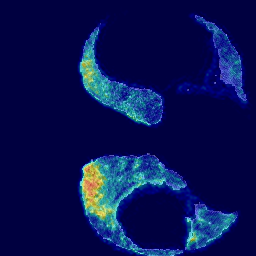
\includegraphics[width=\textwidth]{img/label0_correcto_pred0_pid65HANX_slice_21.png}
    \caption{Slice 21}
\end{subfigure}
\hfill
\begin{subfigure}[b]{0.45\textwidth}
    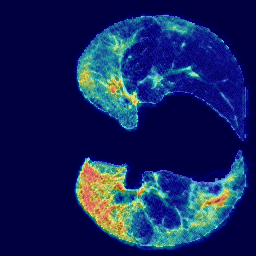
\includegraphics[width=\textwidth]{img/label0_correcto_pred0_pid65HANX_slice_42.png}
    \caption{Slice 42}
\end{subfigure}

\vspace{0.5cm}

\begin{subfigure}[b]{0.45\textwidth}
    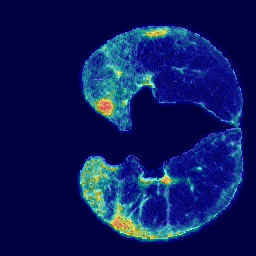
\includegraphics[width=\textwidth]{img/label0_correcto_pred0_pid65HANX_slice_63.png}
    \caption{Slice 63}
\end{subfigure}
\hfill
\begin{subfigure}[b]{0.45\textwidth}
    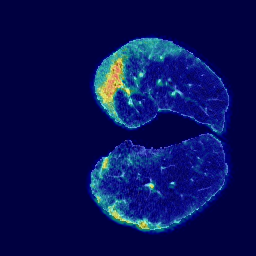
\includegraphics[width=\textwidth]{img/label0_correcto_pred0_pid65HANX_slice_84.png}
    \caption{Slice 84}
\end{subfigure}

\caption{Instancia sin complicación predicha correctamente. Elaboración propia. }
\label{fig:label0-correcta}
\end{figure}

%--------------------------------------------

\begin{figure}[!htbp]
\centering
\begin{subfigure}[b]{0.45\textwidth}
    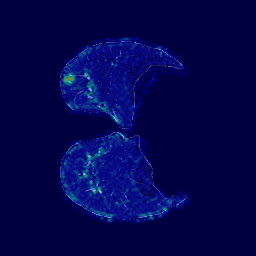
\includegraphics[width=\textwidth]{img/label1_correcto_pred1_pid95HASH_slice_42.png}
    \caption{Slice 42}
\end{subfigure}
\hfill
\begin{subfigure}[b]{0.45\textwidth}
    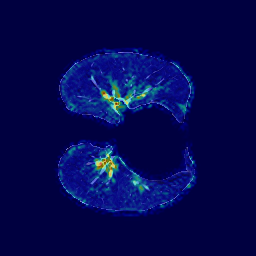
\includegraphics[width=\textwidth]{img/label1_correcto_pred1_pid95HASH_slice_63.png}
    \caption{Slice 63}
\end{subfigure}

\vspace{0.5cm}

\begin{subfigure}[b]{0.45\textwidth}
    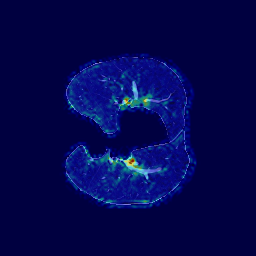
\includegraphics[width=\textwidth]{img/label1_correcto_pred1_pid95HASH_slice_84.png}
    \caption{Slice 84}
\end{subfigure}
\hfill
\begin{subfigure}[b]{0.45\textwidth}
    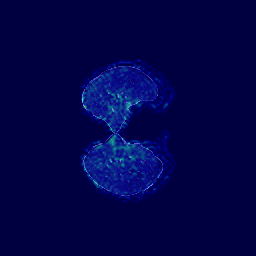
\includegraphics[width=\textwidth]{img/label1_correcto_pred1_pid95HASH_slice_105.png}
    \caption{Slice 105}
\end{subfigure}

\caption{Instancia con complicación predicha correctamente. Tipo de complicación: hemorragia leve. Elaboración propia. }
\label{fig:label1-correcta}
\end{figure}


%-------------------------------

\begin{figure}[!htbp]
\centering
\begin{subfigure}[b]{0.45\textwidth}
    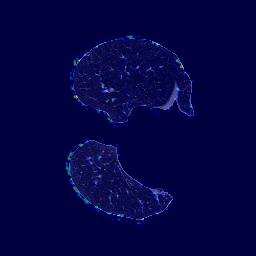
\includegraphics[width=\textwidth]{img/label0_fallo_pred1_pid32HENX_slice_42.png}
    \caption{Slice 42}
\end{subfigure}
\hfill
\begin{subfigure}[b]{0.45\textwidth}
    
\includegraphics[width=\textwidth]{img/label0_fallo_pred1_pid32HENX_slice_63.png}
    \caption{Slice 63}
\end{subfigure}

\vspace{0.5cm}

\begin{subfigure}[b]{0.45\textwidth}
    
\includegraphics[width=\textwidth]{img/label0_fallo_pred1_pid32HENX_slice_84.png}
    \caption{Slice 84}
\end{subfigure}
\hfill
\begin{subfigure}[b]{0.45\textwidth}
    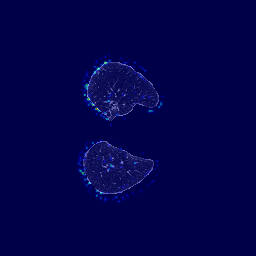
\includegraphics[width=\textwidth]{img/label0_fallo_pred1_pid32HENX_slice_105.png}
    \caption{Slice 105}
\end{subfigure}

\caption{Instancia sin complicación predicha incorrectamente. Elaboración propia. }
\label{fig:label0-incorrecta}
\end{figure}


%----------------------------

\begin{figure}[!htbp]
\centering
\begin{subfigure}[b]{0.45\textwidth}
    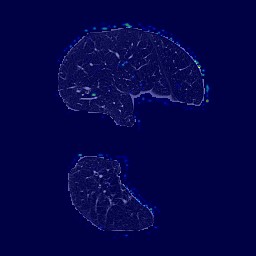
\includegraphics[width=\textwidth]{img/label1_fallo_pred0_pid87MASSN_slice_42.png}
    \caption{Slice 42}
\end{subfigure}
\hfill
\begin{subfigure}[b]{0.45\textwidth}
    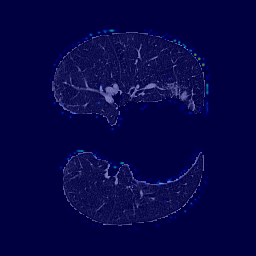
\includegraphics[width=\textwidth]{img/label1_fallo_pred0_pid87MASSN_slice_63.png}
    \caption{Slice 63}
\end{subfigure}

\vspace{0.5cm}

\begin{subfigure}[b]{0.45\textwidth}
    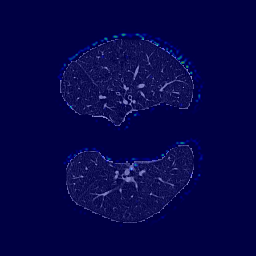
\includegraphics[width=\textwidth]{img/label1_fallo_pred0_pid87MASSN_slice_84.png}
    \caption{Slice 84}
\end{subfigure}
\hfill
\begin{subfigure}[b]{0.45\textwidth}
    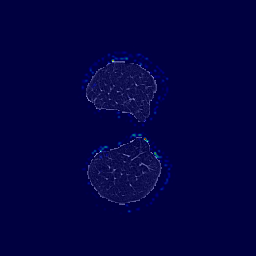
\includegraphics[width=\textwidth]{img/label1_fallo_pred0_pid87MASSN_slice_105.png}
    \caption{Slice 105}
\end{subfigure}

\caption{Instancia sin complicación predicha correctamente. Tipo de complicación: neumotórax y hemorragia. Elaboración propia. }
\label{fig:label1-incorrecta}
\end{figure}




\subsection{Shap}
Queríamos validar los resultados obtenidos con \textit{Grad-CAM} empleando una técnica de explicabilidad complementaria. La idea era comprobar si los mapas de activación generados por \textit{Grad-CAM} reflejaban realmente información significativa sobre el modelo o si, por el contrario, las inconsistencias detectadas se debían a limitaciones de la propia técnica de visualización. Este contraste nos permitiría distinguir si los problemas observados eran debidos a un mal entrenamiento del modelo o a la herramienta de explicabilidad en sí.

Para ello, realizamos una prueba con SHAP (\textit{SHapley Additive exPlanations}), un método de interpretabilidad muy popular por su versatilidad y capacidad para explicar las predicciones de modelos de aprendizaje automático \parencite{ponce2024practical}. Su objetivo es mejorar la transparencia y la confianza en los sistemas de IA, permitiendo comprender cómo el modelo llega a sus decisiones.

SHAP se basa en la teoría de los valores de Shapley para cuantificar la contribución de cada característica a la predicción de un modelo. Para una muestra específica, el valor SHAP de una característica indica en qué medida contribuye a la diferencia entre la predicción individual de esa muestra y la predicción media del modelo.

En el ámbito de las imágenes, SHAP permite visualizar qué regiones son más influyentes para la predicción de un modelo. Dado que un solo píxel no suele ser interpretable por sí mismo, SHAP agrupa los píxeles en segmentos homogéneos llamados \textit{superpíxeles}. Estos superpíxeles se consideran las \textit{características} de entrada para el modelo explicativo de SHAP \parencite{dewi2023xai}.

Sin embargo, en nuestro caso concreto, SHAP no resultó especialmente útil, ya que su salida no era tan interpretable en volúmenes 3D. Por este motivo, tras una prueba inicial, decidimos no emplearlo de forma sistemática en los experimentos y priorizamos el análisis con \textit{Grad-CAM}, que ofrecía mapas de activación más coherentes y comprensibles para el equipo médico.


\section{Análisis explicativo de los modelos radiómicos}

\subsection{Análisis post-hoc con SHAP}

Con el objetivo de extraer conclusiones interpretables de los datos radiómicos, se ha seleccionado la versión del algoritmo \texttt{LightGBM} que mejores resultados dio al utilizar los datos radiómicos combinados con los datos clínicos, y se ha aplicado también la técnica SHAP para estimar la importancia de cada atributo en la clasificación. La experimentación se ha realizado sobre el fold de validación cruzada que mejores resultados obtuvo en test. Se ha aplicado SHAP sobre todos los pacientes de test y se han analizado sus resultados.

En la Figura \ref{fig:shap} podemos ver el análisis global que proporciona SHAP sobre las predicciones realizadas por LightGBM. Es un diagrama de enjambre en el que se muestra el ranking de características más influyentes. En el eje Y se observan las características radiómicas y clínicas ordenadas por importancia, mientras que en el eje X se observa el valor SHAP, o el impacto en la predicción del modelo. Cada punto del diagrama representa a un paciente, y el color representa el valor del atributo en cuestión.

Por ejemplo, podemos observar que el atributo con mayor impacto global en la predicción es una característica radiómica de la matriz GLSZM calculada sobre la imagen mediante una transformación wavelet-HLL. Vemos que hay hasta 4 pacientes que se destacan con un impacto muy alto en la predicción positiva. El color azul además indica que los valores de este atributo en estos pacientes es bajo. Esto nos da la idea de que valores bajos de esa característica radiómica pueden contribuir a una predicción positiva de complicación. En la siguiente característica, \texttt{ngtdm\_Busyness} bajo la transformación logarítmica, observamos también algo interesante. En la frontera de impacto (el valor shap 0), podemos ver que hacia la derecha todos los valores presentan un valor alto del atributo, mientras que a la derecha todos presentan un valor bajo. Esto se podría interpretar como que este atributo es muy influyente en la toma de decisiones, ya que proporciona una predicción positiva siempre que es alto y una predicción negativa siempre que es bajo. En el tercer atributo sucede al contrario, indicando que valores bajos pueden contribuir a la predicción positiva y valores bajos a la negativa. En general, la información de la Figura \ref{fig:shap} puede ser de gran interés clínico, ya que se puede combinar con el conocimiento experto de los médicos para tratar de extraer conclusiones relevantes sobre las características relevantes y su importancia en las predicciones.

Otro aspecto a destacar sobre la Figura \ref{fig:shap} a nivel global es qué tipos de atributos son los más destacados. Podemos ver que predominan las transformaciones wavelet, variando el tipo de filtro empleado en cada eje. En general, las características radiómicas transformadas dominan la gráfica, apareciendo características originales en 2 de las 20 características más destacadas. Esto nos puede indicar que, efectivamente, el uso de características radiómicas obtenidas a partir de las transformaciones de la imagen introduce información relevante en el problema de clasificación. Por otra parte, podemos ver que no llega a verse ninguna característica clínica, pese a que en este modelo se utilizaron características radiómicas y clínicas conjuntamente. Esto nos indica que, para el modelo LightGBM entrenado, los datos clínicos no parecen haber sido especialmente relevantes para determinar una posible complicación o no.

\begin{figure}
    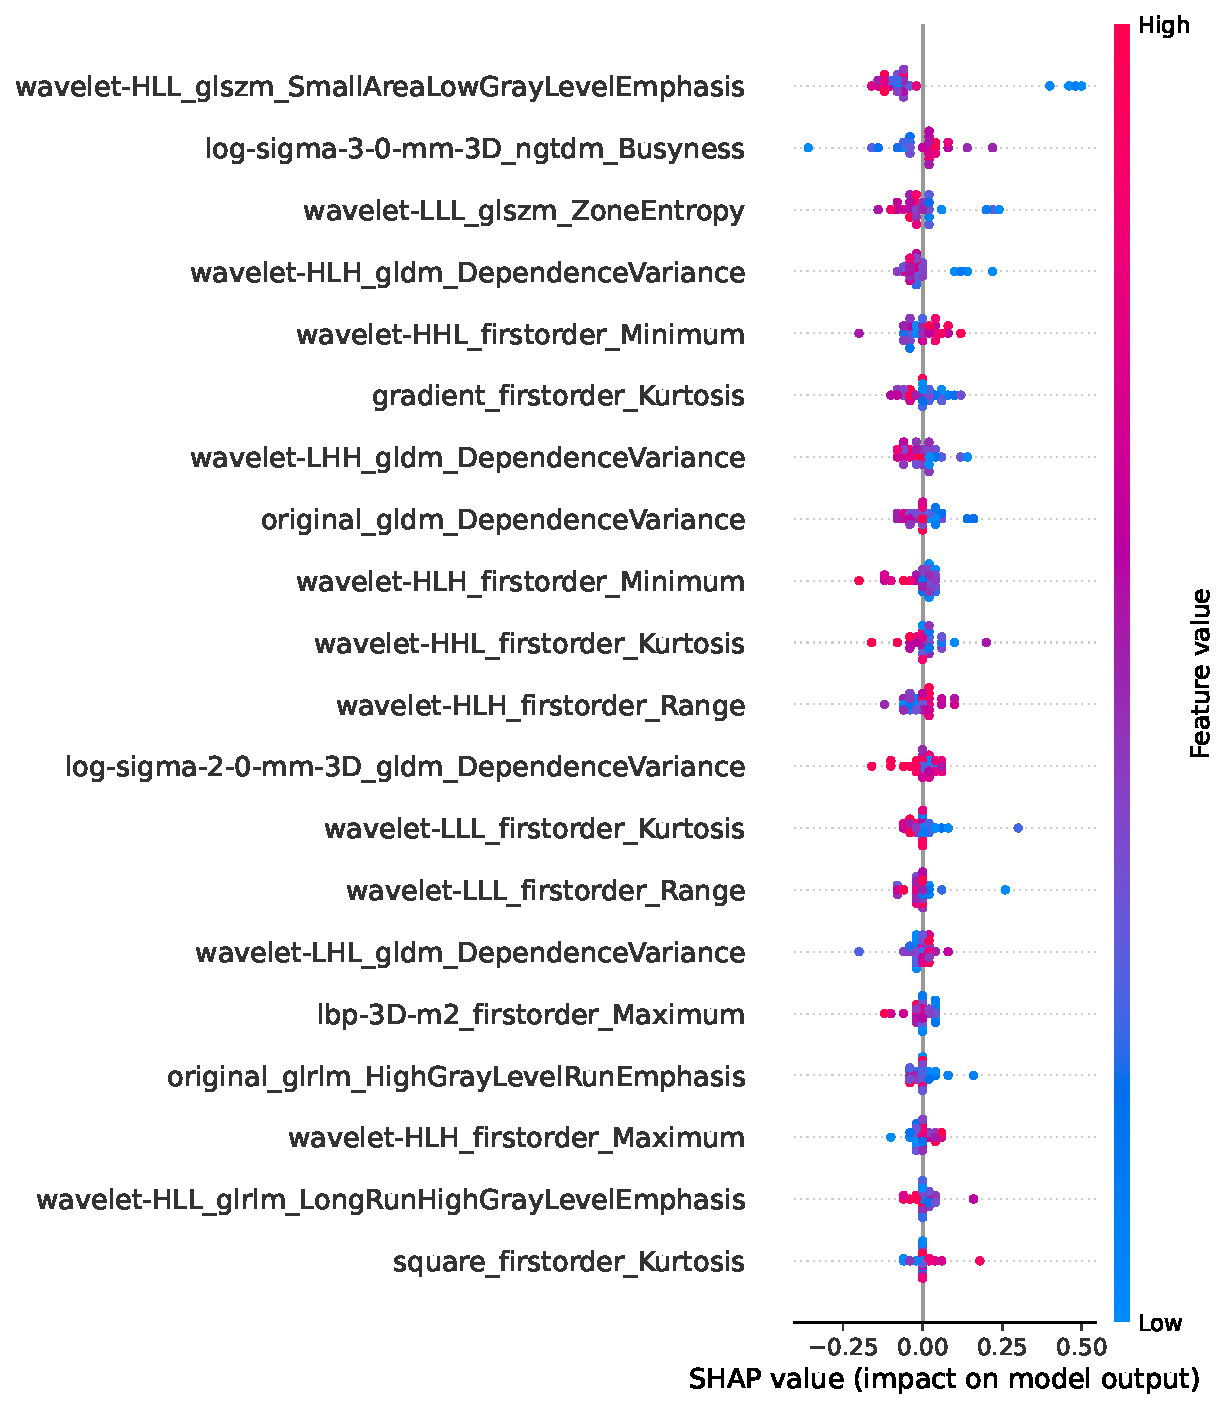
\includegraphics[width=\textwidth]{shap_summary_plot_lighbmg_extended.pdf} \caption{Diagrama resumen de las características más influyentes en la predicción de LightGBM según SHAP.}\label{fig:shap}
    
\end{figure}

Para concluir el análisis de SHAP vamos a realizar un análisis a nivel de paciente. En las Figuras \ref{fig:shap_tn}, \ref{fig:shap_tp} y \ref{fig:shap_f} se muestran, respectivamente, los análisis de SHAP sobre los pacientes predichos correctamente como positivos, como negativos, y los pacientes en los que el algoritmo se ha equivocado. Estas imágenes son gráficos en cascada en los que se representan los atributos más relevantes para cada paciente y el empuje que realizan hacia una predicción positiva (rojo) o negativa (azul). Se parte desde la probabilidad media de predicción de complicación obtenida por el modelo ($E[f(X)] = 0.4$), y los distintos atributos van empujando en una dirección u otra, hasta llegar a la probabilidad final de complicación, que alcanza el 1 en todos los pacientes predichos como positivos y 0 en los negativos. También podemos observar el valor de entrada de cada atributo.

Podemos ver que las características más destacadas del análisis global, como la GLSZM de la transformada wavelet o el \texttt{ngtdm\_Busyness} de la transformada logarítmica, están presentes también individualmente en la mayoría de pacientes. Podemos observar sus valores y confirmar que en las predicciones positivas están con valores bajos y altos, respectivamente, y al revés en las predicciones positivas. También es interesante observar que, como es de esperar, en las predicciones positivas predominan los atributos que empujan hacia la clase positiva (en rojo), mientras que en las negativas predominan los atributos que empujan hacia la negativa (azul).Sin embargo, siempre podemos identificar ciertos atributos que empujan hacia la clase contraria. Estos atributos pueden entenderse como señales de alerta: aunque el modelo ha tomado una decisión concreta, ha percibido cierta información que puede contener evidencias de pertenencia a la clase contraria. Estas características, pueden analizarse desde el punto de vista médico para corroborar o poner en duda las decisiones tomadas por el modelo, y así actuar convenientemente. Podemos observar además que muchas veces los patrones de alerta son comunes en todos los pacientes. Por ejemplo, en muchos pacientes, podemos ver atributos de primer orden como la curtosis, el mínimo o el máximo suelen empujar hacia la clase contraria a la predicha.

Por último, si nos fijamos en los falsos positivos y falsos negativos, a priori no se observa ningún patrón diferente con respecto a las predicciones correctas. Los atributos siguen empujando en su mayoría hacia la clase predicha, con ciertas excepciones, aunque en estos casos observamos que entre las señales de alerta no aparecen tanto curtosis, máximos y mínimos. Lo que sí que vemos es que las características predominantes a nivel global son dominantes en estos ejemplos y, posiblemente, son determinantes en la toma de la decisión errónea por parte del modelo.





% ============================================
% PRIMERA PÁGINA - VERDADEROS NEGATIVOS
% ============================================
\begin{figure}[p]
    \centering
    

    \medskip
    \foreach \i in {0,4,5,6,7,8,9,13,15,16,17,20,22}{
        \begin{subfigure}[b]{0.45\textwidth}
            \includegraphics[width=\linewidth]{patient_\i_label_0_pred_0.pdf}
        \end{subfigure}
    }

    \caption{Análisis de SHAP de los pacientes clasificados correctamente como negativos.}\label{fig:shap_tn}

\end{figure}


% ============================================
% SEGUNDA PÁGINA - VERDADEROS POSITIVOS
% ============================================
\begin{figure}[p]
    \centering

    \medskip
    \foreach \i in {2,3,10,14,18,19,21,23,24}{
        \begin{subfigure}[b]{0.47\textwidth}
            \includegraphics[width=\linewidth]{patient_\i_label_1_pred_1.pdf}
        \end{subfigure}
    }
    \caption{Análisis de SHAP de los pacientes clasificados correctamente como positivos.}\label{fig:shap_tp}
\end{figure}

\clearpage

% ============================================
% TERCERA PÁGINA - FALSOS POSITIVOS Y FALSOS NEGATIVOS
% ============================================
\begin{figure}[p]
    \centering
    % --- Falsos Positivos ---
    \vspace{0.5cm}
    \textbf{Falso Positivo}

    \medskip
    \foreach \i in {1}{
        \begin{subfigure}[b]{0.47\textwidth}
            \includegraphics[width=\linewidth]{patient_\i_label_0_pred_1.pdf}
        \end{subfigure}
    }

    % --- Falsos Negativos ---
    \vspace{0.8cm}
    \textbf{Falsos Negativos}

    \medskip
    \foreach \i in {11,12}{
        \begin{subfigure}[b]{0.47\textwidth}
            \includegraphics[width=\linewidth]{patient_\i_label_1_pred_0.pdf}
        \end{subfigure}
    }

    \caption{Análisis de SHAP de los pacientes clasificados incorrectamente.}\label{fig:shap_f}

\end{figure}

\subsection{Discusión de aproximaciones alternativas}

En la experimentación con datos radiómicos se probó a utilizar árboles de decisión, algoritmos que por naturaleza son explicables. Sin embargo, no obtuvieron resultados demasiado buenos. Sí hubo una combinación razonable que alcanzó un 0.67 de F1 y 0.7 de G-Mean, aunque este fue aplicado sobre un preprocesamiento con PCA al 95 \% de la varianza. Por tanto, la información que obtiene el árbol de decisión es a partir de dichas componentes principales, en lugar de las características radiómicas. Por tanto, para poder hacer un análisis explicativo razonable habría que analizar en primer lugar dichas componentes principales y ver qué atributos se combinan mayoritariamente en cada componente, lo cual tiene una complejidad elevada. En la Figura \ref{fig:expl_arbol} se muestra la secuencia de divisiones realizadas por el árbol de decisión aprendido para determinar la clase a partir de las componentes principales.

\begin{figure}
    \includegraphics[width=\textwidth]{arbol_decision.pdf} \caption{Análisis de la toma de decisiones mejor modelo de árbol de decisión obtenido en función de las componentes principales extraídas.}\label{fig:expl_arbol}
\end{figure}

Por último, dada la especial relevancia que han tenido los algoritmos basados en distancias en la experimentación radiómica, es relevante comentar que en las implementaciones de $k$-NN podemos analizar los vecinos más cercanos que se han utilizado para la toma de una decisión concreta. Desde el punto de vista médico, los expertos médicos podrían en estas situaciones analizar los TC y datos clínicos de los ejemplos ya conocidos que han sido marcados como los más similares al ejemplo a predecir, y corroborar o descartar la decisión del modelo apoyándose en su juicio médico.


\endinput
%--------------------------------------------------------------------
% FIN DEL CAPÍTULO. 
%--------------------------------------------------------------------


\cleardoublepage\part{Conclusiones}
% !TeX root = ../tfg.tex
% !TeX encoding = utf8

\chapter{Conclusiones}
En este trabajo, se ha abordado el problema de la predicción de complicaciones en biopsias de pulmón, un problema novedoso y de interés médico, que en caso de abordarse exitosamente puede suponer un avance importante en el campo de toma de muestras de tejido pulmonar, al anticipar los posibles riesgos que puedan producirse. Para realizar este se ha trabajado, se ha colaborado con un equipo médico del Hospital San Cecilio, el cual ha proporcionado datos etiquetados y conocimiento experto para abordar este problema.

El trabajo se ha abordado desde dos perspectivas: una matemática, en la que se han analizado los fundamentos de las técnicas que se han empleado en el problema a tratar, y una informática, en la que se describen las distintas formas en las que se ha intentado abordar el problema. En los fundamentos teóricos se han analizado conceptos como la teoría de la señal aplicada a imágenes, optimización y fundamentos teóricos del aprendizaje automático, profundo y de métricas de distancia. El problema práctico de la predicción de complicaciones se ha abordado empleando distintas técnicas, tanto de deep learning (en 2 y 3 dimensiones) como de radiómica, pasando también por un análisis de los datos proporcionados, un preprocesamiento adecuada y un post-análisis donde se intentan analizar las decisiones tomadas por los modelos.

Durante buena parte del desarrollo del proyecto, los resultados fueron nulos o claramente insuficientes, hasta el punto de cuestionarnos si el problema era abordable con los recursos disponibles. La progresiva recolección de más datos ayudó a mejorar el rendimiento, pero el avance fue siempre desafiante: al principio sufríamos un marcado desbalance de clases, más tarde se resolvió parcialmente, pero aparecían otros problemas como la ausencia de segmentación o el uso de imágenes de tamaños demasiado grandes. Fue especialmente revelador incluir técnicas de explicabilidad, que nos mostraron que el modelo no se fijaba en las regiones pulmonares relevantes, motivándonos a segmentar y a reducir el tamaño de las imágenes para centrar la atención del modelo en lo importante.

Uno de los mayores avances fue el paso a modelos 3D, ya que las aproximaciones iniciales en 2D no funcionaban de forma efectiva. La combinación de segmentación pulmonar, reducción de tamaño y el procesamiento en 3D permitió extraer características más informativas, aunque incluso así los resultados obtenidos con modelos volumétricos puros (DenseNet121 entrenado desde cero, preentrenado o en versiones híbridas con datos clínicos) quedaron lejos de ser satisfactorios. El preentrenamiento en dominios diferentes o la fusión multimodal con datos clínicos no lograron superar los problemas de sobreajuste ni las limitaciones derivadas del reducido tamaño del conjunto de datos.

Ante estas limitaciones del deep learning, atribuibles en gran medida a la escasez de datos y la complejidad del problema, se decidió explorar estrategias más clásicas. Así, se desarrolló un enfoque basado en radiómica, extrayendo características cuantitativas de los volúmenes para alimentar modelos de aprendizaje automático convencional. Esta estrategia resultó ser significativamente más robusta: incluso sin incluir datos clínicos ni metric learning, la radiómica pura logró resultados notablemente mejores que los modelos volumétricos puros o basados solo en datos tabulares.

La incorporación de datos clínicos aportó una mejora adicional, demostrando el valor predictivo complementario de la información del paciente. Además, el uso de técnicas de metric learning permitió aprender representaciones más discriminativas, alcanzando resultados comparables incluso sin datos clínicos. Finalmente, la combinación de radiómica, datos clínicos y metric learning se consolidó como la mejor estrategia, logrando el mayor rendimiento global con un G-Mean aproximado del 74\% en test. Este resultado demuestra un equilibrio sólido entre sensibilidad y especificidad, validando la efectividad de integrar diferentes fuentes de información y técnicas de aprendizaje.

En conclusión, este trabajo evidencia que el deep learning puro no siempre es la opción más adecuada, especialmente en contextos con datos limitados y problemas clínicos complejos. La estrategia de extraer características radiómicas y aplicar aprendizaje automático clásico se ha mostrado más efectiva en este escenario, ofreciendo una solución más interpretable, menos exigente en datos y con mejor rendimiento final para la tarea de predicción de complicaciones en biopsias pulmonares. El problema abordado, si bien con las últimas aproximaciones se han conseguido mejoras relevantes en los resultados, aún deja un amplio margen de mejora. El problema de predicción de complicaciones en biopsias presenta un gran interés clínico y humano, y por ello se espera que la investigación realizada en este trabajo sirva como base para continuar profundizando en la obtención de modelos aún más efectivos.

\section{Líneas de trabajo futuro}

A partir de los resultados obtenidos y de las limitaciones identificadas durante el desarrollo del proyecto, se plantean varias líneas de trabajo futuro para mejorar el rendimiento del modelo:

\begin{itemize}
    \item \textbf{Abordar la predicción del tipo de complicación}: es una extensión natural del problema actual.  Consistiría en abordar no solo la predicción binaria de complicación o no complicación, sino la clasificación del tipo específico de complicación, formulada como un problema de clasificación multietiqueta. Para ello sería indispensable disponer de más datos, ya que en el dataset actual hay tipos de complicaciones con muy pocos casos (incluso un solo ejemplo), lo que hace inabordable el entrenamiento en este momento.
    \item \textbf{Ajustar la segmentación a estructuras más relevantes dentro del pulmón}: en cuanto al preprocesamiento, se propone avanzar hacia segmentaciones más precisas y orientadas a estructuras anatómicas clave como tumores y vasos sanguíneos. Esto permitiría al modelo centrarse en la información más relevante para la predicción. Además, se sugiere investigar hipótesis clínicas planteadas por los propios especialistas, como la posible relación entre el tamaño de la lesión y el riesgo de complicación (por ejemplo, lesiones más pequeñas podrían implicar mayor dificultad técnica en la biopsia).
    \item \textbf{Aprendizaje federado e integración de datos de distintos hospitales}: pueden permitir entrenar modelos de forma colaborativa entre distintos hospitales sin necesidad de compartir datos sensibles. Esto facilitaría el acceso a conjuntos de datos más grandes y diversos, garantizando al mismo tiempo la privacidad de los pacientes.
    \item \textbf{Análisis del impacto de variables técnicas}, como el modelo de máquina de TC utilizada para las adquisiciones. Diferencias en la resolución o en los parámetros de imagen pueden afectar al rendimiento del modelo, que podría aprender a discriminar entre máquinas en lugar de entre patrones clínicos reales, comprometiendo su capacidad de generalización.
    \item \textbf{Aprendizaje con mecanismos de atención}: se plantea también integrar mecanismos de atención en los modelos para reforzar su capacidad de focalizarse en regiones importantes de la imagen y mejorar la interpretabilidad de las predicciones. Incluso, avanzar en técnicas de explicabilidad será clave para generar confianza clínica y facilitar la validación del sistema en entornos reales.
    \item \textbf{Aproximaciones semisupervisadas}: por último, se propone investigar estrategias semisupervisadas que permitan aprovechar tanto datos de pacientes sanos como datos de pacientes con tumores que no estén etiquetados con las complicaciones en biopsias, lo que permitiría entrenar con una cantidad más abundante de datos.
\end{itemize}

\endinput
%--------------------------------------------------------------------
% FIN DEL CAPÍTULO. 
%--------------------------------------------------------------------


% -------------------------------------------------------------------
% APPENDIX: Opcional
% -------------------------------------------------------------------

% \appendix % Reinicia la numeración de los capítulos y usa letras para numerarlos
% \pdfbookmark[-1]{Apéndices}{appendix} % Alternativamente podemos agrupar los apéndices con un nuevo \part{Apéndices}

% % !TeX root = ../tfg.tex
% !TeX encoding = utf8

\chapter{Ejemplo de apéndice}\label{ap:apendice1}

Los apéndices son opcionales.

Este fichero \texttt{apendice-ejemplo.tex} es una plantilla para añadir apéndices al \textsc{tfg}. Para ello, es necesario:
\begin{itemize}
  \item Crear una copia de este fichero \texttt{apendice-ejemplo.tex} en la carpeta \texttt{apendices} con un nombre apropiado (p.e. \texttt{apendice01.tex}).
  \item Añadir el comando \texttt{$\backslash$input\{apendices/apendice01\}} en el fichero principal \texttt{tfg.tex} donde queremos que aparezca dicho apéndice (debe de ser después del comando \texttt{$\backslash$appendix}).
\end{itemize}

\endinput
%------------------------------------------------------------------------------------
% FIN DEL APÉNDICE. 
%------------------------------------------------------------------------------------

% Añadir tantos apéndices como sea necesario 

% -------------------------------------------------------------------
% GLOSARIO: Opcional
% -------------------------------------------------------------------

% !TeX root = ../tfg.tex
% !TeX encoding = utf8

\chapter*{Glosario}
\addcontentsline{toc}{chapter}{Glosario} % Añade el glosario a la tabla de contenidos


\begin{description}
  \item $\mathbb{R}$: Conjunto de números reales.
  \item $\mathbb{Z}$: Conjunto de números enteros.
  \item $\mathbb{R}^n$: Espacio euclídeo n-dimensional.
  \item $\mathbb{R}^{n \times m}$: Conjunto de matrices reales de tamaño $n \times m$.
  \item \textbf{TC}: Tomografía Computarizada
  \item \textbf{IA}: Inteligencia Artificial
  \item \textbf{BAG}: Biopsia por aguja gruesa
  \item \textbf{CT-guided PTNB}: Biopsia pulmonar transtorácica con aguja guiada por TC
  \item \textbf{MSE}: Error cuadrático medio (Mean Squared Error)
  \item \textbf{DFT}: Transformada Discreta de Fourier
  \item \textbf{FFT}: Transformada Rápida de Fourier
  \item \textbf{p.c.t}: para casi todo
  \item \textbf{c.p.d}: casi por doquier
  \item \textbf{ReLU}: Rectified Linear Units
  \item \textbf{PReLU}: Parametric ReLU
  \item \textbf{CNNs}: Convolutional Neural Networks
  \item \textbf{PCA}: Análisis de componentes principales (Principal Component Analysis)
  \item \textbf{NCA}: Neigborhood Components Analysis
  \item \textbf{LMNN}: Large Margin Nearest Neighbors
  \item \textbf{k-NN}: k-nearest neighbors
  \item \textbf{DML}: Aprendizaje de métricas profundo (Distance metric learning)
  \item \textbf{SVM}: Máquinas de vectores soporte (Support Vector Machines)
  \item \textbf{DICOM}: Digital Imaging and Communication in Medicine
  \item \textbf{NIfTI}: Neuroimaging Informatics Technology Initiative
  \item \textbf{RGPD}: Reglamento General de Protección de Datos (Reglamento (UE) 2016/679)
  \item \textbf{AEPD}: Agencia Española de Protección de Datos
  \item \textbf{EDA}: Análisis exploratorio de datos
  \item \textbf{GPUs}: Graphics Processing Units
  \item \textbf{MONAI}: Medical Open Network for Artificial Intelligence
  \item \textbf{IBSI}: Image Biomarker Standardisation Initiative
  \item \textbf{ROI}: Regiones de interés (Region of Interest)
  \item \textbf{VOI}: Volúmenes de interés (Volume of Interest)
  \item \textbf{HU}: Unidades Hounsfield
  \item \textbf{MLP}: Red neuronal multicapa (Multi-Layer Perceptron)
  \item \textbf{GLCM}: Matrices de co-ocurrencia de niveles de gris
  \item \textbf{GLDM}: Matriz de diferencia de niveles de gris
  \item \textbf{GLRLM}: Matrices de longitud de recorrido de niveles de gris
  \item \textbf{GLSZM}: Matriz de zonas de tamaño de niveles de gris
  \item \textbf{MPR}: Reformateo Multiplanar
  \item \textbf{TPR}: True Positive Rate (Sensibilidad)
  \item \textbf{TNR}: True Negative Rate (Especificidad)
  \item \textbf{DAG}: Grafo dirigido acíclico (Directed Acyclic Graph)
  \item \textbf{SHAP}: SHapley Additive exPlanations
  \item \textbf{TFG}: Trabajo de Fin de Grado
  \item \textbf{DL}: Deep Learning
  \item \textbf{ResNet}: Residual Networks
  \item \textbf{DenseNet}: Densely Connected Convolutional Network
  \item \textbf{CPU}: Procesador
  \item \textbf{UGR}: Universidad de Granada
  \item \textbf{NGPU}: Servidores de cómputo de alto rendimiento
  \item \textbf{WL}: Window Level
  \item \textbf{WW}: Window Width
  \item \textbf{IHC}: Inmunohistoquímica
  \item \textbf{DC}: Frecuencia cero, brillo medio en toda la imagen
\end{description}

\endinput

 

% -------------------------------------------------------------------
% BACKMATTER
% -------------------------------------------------------------------

\backmatter % Desactiva la numeración de los capítulos
\pdfbookmark[-1]{Referencias}{BM-Referencias}

% BIBLIOGRAFÍA
%-------------------------------------------------------------------
\printbibliography

\end{document}
